%%%%%%%%%%%%%%%%%%%%%%%%%%%%%% -*- Mode: Latex -*- %%%%%%%%%%%%%%%%%%%%%%%%%%%%
%% 07-04.tex -- Dissertation for Ph.D
%% Author          : Hongbing Kou
%% Created On      : Mon Sep 23 11:52:28 2002
%% Last Modified By: Hongbing Kou
%% Last Modified On: Fri Sep  7 11:22:55 2007
%% RCS: $Id$
%%%%%%%%%%%%%%%%%%%%%%%%%%%%%%%%%%%%%%%%%%%%%%%%%%%%%%%%%%%%%%%%%%%%%%%%%%%%%%%
%%   Copyright (C) 2007 Hongbing Kou
%%%%%%%%%%%%%%%%%%%%%%%%%%%%%%%%%%%%%%%%%%%%%%%%%%%%%%%%%%%%%%%%%%%%%%%%%%%%%%%
%% 

%%\documentclass[11pt,twocolumn]{article}
\documentclass[11pt,oneside,final,times,dissertation,actual]{uhthesis2e}
% 10pt, 11pt, 12pt
% oneside, twoside
% draft, final
% cm, times, palatino, newcent, bookman
% dissertation, thesis
% actual, proposal
% substitute ``final'' for ``proposal'' to get actual thesis

% Psfig/TeX 
\def\PsfigVersion{1.9}
% dvips version
%
% All psfig/tex software, documentation, and related files
% in this distribution of psfig/tex are 
% Copyright 1987, 1988, 1991 Trevor J. Darrell
%
% Permission is granted for use and non-profit distribution of psfig/tex 
% providing that this notice is clearly maintained. The right to
% distribute any portion of psfig/tex for profit or as part of any commercial
% product is specifically reserved for the author(s) of that portion.
%
% *** Feel free to make local modifications of psfig as you wish,
% *** but DO NOT post any changed or modified versions of ``psfig''
% *** directly to the net. Send them to me and I'll try to incorporate
% *** them into future versions. If you want to take the psfig code 
% *** and make a new program (subject to the copyright above), distribute it, 
% *** (and maintain it) that's fine, just don't call it psfig.
%
% Bugs and improvements to trevor@media.mit.edu.
%
% Thanks to Greg Hager (GDH) and Ned Batchelder for their contributions
% to the original version of this project.
%
% Modified by J. Daniel Smith on 9 October 1990 to accept the
% %%BoundingBox: comment with or without a space after the colon.  Stole
% file reading code from Tom Rokicki's EPSF.TEX file (see below).
%
% More modifications by J. Daniel Smith on 29 March 1991 to allow the
% the included PostScript figure to be rotated.  The amount of
% rotation is specified by the "angle=" parameter of the \psfig command.
%
% Modified by Robert Russell on June 25, 1991 to allow users to specify
% .ps filenames which don't yet exist, provided they explicitly provide
% boundingbox information via the \psfig command. Note: This will only work
% if the "file=" parameter follows all four "bb???=" parameters in the
% command. This is due to the order in which psfig interprets these params.
%
%  3 Jul 1991	JDS	check if file already read in once
%  4 Sep 1991	JDS	fixed incorrect computation of rotated
%			bounding box
% 25 Sep 1991	GVR	expanded synopsis of \psfig
% 14 Oct 1991	JDS	\fbox code from LaTeX so \psdraft works with TeX
%			changed \typeout to \ps@typeout
% 17 Oct 1991	JDS	added \psscalefirst and \psrotatefirst
%

% From: gvr@cs.brown.edu (George V. Reilly)
%
% \psdraft	draws an outline box, but doesn't include the figure
%		in the DVI file.  Useful for previewing.
%
% \psfull	includes the figure in the DVI file (default).
%
% \psscalefirst width= or height= specifies the size of the figure
% 		before rotation.
% \psrotatefirst (default) width= or height= specifies the size of the
% 		 figure after rotation.  Asymetric figures will
% 		 appear to shrink.
%
% \psfigurepath#1	sets the path to search for the figure
%
% \psfig
% usage: \psfig{file=, figure=, height=, width=,
%			bbllx=, bblly=, bburx=, bbury=,
%			rheight=, rwidth=, clip=, angle=, silent=}
%
%	"file" is the filename.  If no path name is specified and the
%		file is not found in the current directory,
%		it will be looked for in directory \psfigurepath.
%	"figure" is a synonym for "file".
%	By default, the width and height of the figure are taken from
%		the BoundingBox of the figure.
%	If "width" is specified, the figure is scaled so that it has
%		the specified width.  Its height changes proportionately.
%	If "height" is specified, the figure is scaled so that it has
%		the specified height.  Its width changes proportionately.
%	If both "width" and "height" are specified, the figure is scaled
%		anamorphically.
%	"bbllx", "bblly", "bburx", and "bbury" control the PostScript
%		BoundingBox.  If these four values are specified
%               *before* the "file" option, the PSFIG will not try to
%               open the PostScript file.
%	"rheight" and "rwidth" are the reserved height and width
%		of the figure, i.e., how big TeX actually thinks
%		the figure is.  They default to "width" and "height".
%	The "clip" option ensures that no portion of the figure will
%		appear outside its BoundingBox.  "clip=" is a switch and
%		takes no value, but the `=' must be present.
%	The "angle" option specifies the angle of rotation (degrees, ccw).
%	The "silent" option makes \psfig work silently.
%

% check to see if macros already loaded in (maybe some other file says
% "\input psfig") ...
\ifx\undefined\psfig\else\endinput\fi

%
% from a suggestion by eijkhout@csrd.uiuc.edu to allow
% loading as a style file. Changed to avoid problems
% with amstex per suggestion by jbence@math.ucla.edu

\let\LaTeXAtSign=\@
\let\@=\relax
\edef\psfigRestoreAt{\catcode`\@=\number\catcode`@\relax}
%\edef\psfigRestoreAt{\catcode`@=\number\catcode`@\relax}
\catcode`\@=11\relax
\newwrite\@unused
\def\ps@typeout#1{{\let\protect\string\immediate\write\@unused{#1}}}
\ps@typeout{psfig/tex \PsfigVersion}

%% Here's how you define your figure path.  Should be set up with null
%% default and a user useable definition.

\def\figurepath{./}
\def\psfigurepath#1{\edef\figurepath{#1}}

%
% @psdo control structure -- similar to Latex @for.
% I redefined these with different names so that psfig can
% be used with TeX as well as LaTeX, and so that it will not 
% be vunerable to future changes in LaTeX's internal
% control structure,
%
\def\@nnil{\@nil}
\def\@empty{}
\def\@psdonoop#1\@@#2#3{}
\def\@psdo#1:=#2\do#3{\edef\@psdotmp{#2}\ifx\@psdotmp\@empty \else
    \expandafter\@psdoloop#2,\@nil,\@nil\@@#1{#3}\fi}
\def\@psdoloop#1,#2,#3\@@#4#5{\def#4{#1}\ifx #4\@nnil \else
       #5\def#4{#2}\ifx #4\@nnil \else#5\@ipsdoloop #3\@@#4{#5}\fi\fi}
\def\@ipsdoloop#1,#2\@@#3#4{\def#3{#1}\ifx #3\@nnil 
       \let\@nextwhile=\@psdonoop \else
      #4\relax\let\@nextwhile=\@ipsdoloop\fi\@nextwhile#2\@@#3{#4}}
\def\@tpsdo#1:=#2\do#3{\xdef\@psdotmp{#2}\ifx\@psdotmp\@empty \else
    \@tpsdoloop#2\@nil\@nil\@@#1{#3}\fi}
\def\@tpsdoloop#1#2\@@#3#4{\def#3{#1}\ifx #3\@nnil 
       \let\@nextwhile=\@psdonoop \else
      #4\relax\let\@nextwhile=\@tpsdoloop\fi\@nextwhile#2\@@#3{#4}}
% 
% \fbox is defined in latex.tex; so if \fbox is undefined, assume that
% we are not in LaTeX.
% Perhaps this could be done better???
\ifx\undefined\fbox
% \fbox code from modified slightly from LaTeX
\newdimen\fboxrule
\newdimen\fboxsep
\newdimen\ps@tempdima
\newbox\ps@tempboxa
\fboxsep = 3pt
\fboxrule = .4pt
\long\def\fbox#1{\leavevmode\setbox\ps@tempboxa\hbox{#1}\ps@tempdima\fboxrule
    \advance\ps@tempdima \fboxsep \advance\ps@tempdima \dp\ps@tempboxa
   \hbox{\lower \ps@tempdima\hbox
  {\vbox{\hrule height \fboxrule
          \hbox{\vrule width \fboxrule \hskip\fboxsep
          \vbox{\vskip\fboxsep \box\ps@tempboxa\vskip\fboxsep}\hskip 
                 \fboxsep\vrule width \fboxrule}
                 \hrule height \fboxrule}}}}
\fi
%
%%%%%%%%%%%%%%%%%%%%%%%%%%%%%%%%%%%%%%%%%%%%%%%%%%%%%%%%%%%%%%%%%%%
% file reading stuff from epsf.tex
%   EPSF.TEX macro file:
%   Written by Tomas Rokicki of Radical Eye Software, 29 Mar 1989.
%   Revised by Don Knuth, 3 Jan 1990.
%   Revised by Tomas Rokicki to accept bounding boxes with no
%      space after the colon, 18 Jul 1990.
%   Portions modified/removed for use in PSFIG package by
%      J. Daniel Smith, 9 October 1990.
%
\newread\ps@stream
\newif\ifnot@eof       % continue looking for the bounding box?
\newif\if@noisy        % report what you're making?
\newif\if@atend        % %%BoundingBox: has (at end) specification
\newif\if@psfile       % does this look like a PostScript file?
%
% PostScript files should start with `%!'
%
{\catcode`\%=12\global\gdef\epsf@start{%!}}
\def\epsf@PS{PS}
%
\def\epsf@getbb#1{%
%
%   The first thing we need to do is to open the
%   PostScript file, if possible.
%
\openin\ps@stream=#1
\ifeof\ps@stream\ps@typeout{Error, File #1 not found}\else
%
%   Okay, we got it. Now we'll scan lines until we find one that doesn't
%   start with %. We're looking for the bounding box comment.
%
   {\not@eoftrue \chardef\other=12
    \def\do##1{\catcode`##1=\other}\dospecials \catcode`\ =10
    \loop
       \if@psfile
	  \read\ps@stream to \epsf@fileline
       \else{
	  \obeyspaces
          \read\ps@stream to \epsf@tmp\global\let\epsf@fileline\epsf@tmp}
       \fi
       \ifeof\ps@stream\not@eoffalse\else
%
%   Check the first line for `%!'.  Issue a warning message if its not
%   there, since the file might not be a PostScript file.
%
       \if@psfile\else
       \expandafter\epsf@test\epsf@fileline:. \\%
       \fi
%
%   We check to see if the first character is a % sign;
%   if so, we look further and stop only if the line begins with
%   `%%BoundingBox:' and the `(atend)' specification was not found.
%   That is, the only way to stop is when the end of file is reached,
%   or a `%%BoundingBox: llx lly urx ury' line is found.
%
          \expandafter\epsf@aux\epsf@fileline:. \\%
       \fi
   \ifnot@eof\repeat
   }\closein\ps@stream\fi}%
%
% This tests if the file we are reading looks like a PostScript file.
%
\long\def\epsf@test#1#2#3:#4\\{\def\epsf@testit{#1#2}
			\ifx\epsf@testit\epsf@start\else
\ps@typeout{Warning! File does not start with `\epsf@start'.  It may not be a PostScript file.}
			\fi
			\@psfiletrue} % don't test after 1st line
%
%   We still need to define the tricky \epsf@aux macro. This requires
%   a couple of magic constants for comparison purposes.
%
{\catcode`\%=12\global\let\epsf@percent=%\global\def\epsf@bblit{%BoundingBox}}
%
%
%   So we're ready to check for `%BoundingBox:' and to grab the
%   values if they are found.  We continue searching if `(at end)'
%   was found after the `%BoundingBox:'.
%
\long\def\epsf@aux#1#2:#3\\{\ifx#1\epsf@percent
   \def\epsf@testit{#2}\ifx\epsf@testit\epsf@bblit
	\@atendfalse
        \epsf@atend #3 . \\%
	\if@atend	
	   \if@verbose{
		\ps@typeout{psfig: found `(atend)'; continuing search}
	   }\fi
        \else
        \epsf@grab #3 . . . \\%
        \not@eoffalse
        \global\no@bbfalse
        \fi
   \fi\fi}%
%
%   Here we grab the values and stuff them in the appropriate definitions.
%
\def\epsf@grab #1 #2 #3 #4 #5\\{%
   \global\def\epsf@llx{#1}\ifx\epsf@llx\empty
      \epsf@grab #2 #3 #4 #5 .\\\else
   \global\def\epsf@lly{#2}%
   \global\def\epsf@urx{#3}\global\def\epsf@ury{#4}\fi}%
%
% Determine if the stuff following the %%BoundingBox is `(atend)'
% J. Daniel Smith.  Copied from \epsf@grab above.
%
\def\epsf@atendlit{(atend)} 
\def\epsf@atend #1 #2 #3\\{%
   \def\epsf@tmp{#1}\ifx\epsf@tmp\empty
      \epsf@atend #2 #3 .\\\else
   \ifx\epsf@tmp\epsf@atendlit\@atendtrue\fi\fi}


% End of file reading stuff from epsf.tex
%%%%%%%%%%%%%%%%%%%%%%%%%%%%%%%%%%%%%%%%%%%%%%%%%%%%%%%%%%%%%%%%%%%

%%%%%%%%%%%%%%%%%%%%%%%%%%%%%%%%%%%%%%%%%%%%%%%%%%%%%%%%%%%%%%%%%%%
% trigonometry stuff from "trig.tex"
\chardef\psletter = 11 % won't conflict with \begin{letter} now...
\chardef\other = 12

\newif \ifdebug %%% turn me on to see TeX hard at work ...
\newif\ifc@mpute %%% don't need to compute some values
\c@mputetrue % but assume that we do

\let\then = \relax
\def\r@dian{pt }
\let\r@dians = \r@dian
\let\dimensionless@nit = \r@dian
\let\dimensionless@nits = \dimensionless@nit
\def\internal@nit{sp }
\let\internal@nits = \internal@nit
\newif\ifstillc@nverging
\def \Mess@ge #1{\ifdebug \then \message {#1} \fi}

{ %%% Things that need abnormal catcodes %%%
	\catcode `\@ = \psletter
	\gdef \nodimen {\expandafter \n@dimen \the \dimen}
	\gdef \term #1 #2 #3%
	       {\edef \t@ {\the #1}%%% freeze parameter 1 (count, by value)
		\edef \t@@ {\expandafter \n@dimen \the #2\r@dian}%
				   %%% freeze parameter 2 (dimen, by value)
		\t@rm {\t@} {\t@@} {#3}%
	       }
	\gdef \t@rm #1 #2 #3%
	       {{%
		\count 0 = 0
		\dimen 0 = 1 \dimensionless@nit
		\dimen 2 = #2\relax
		\Mess@ge {Calculating term #1 of \nodimen 2}%
		\loop
		\ifnum	\count 0 < #1
		\then	\advance \count 0 by 1
			\Mess@ge {Iteration \the \count 0 \space}%
			\Multiply \dimen 0 by {\dimen 2}%
			\Mess@ge {After multiplication, term = \nodimen 0}%
			\Divide \dimen 0 by {\count 0}%
			\Mess@ge {After division, term = \nodimen 0}%
		\repeat
		\Mess@ge {Final value for term #1 of 
				\nodimen 2 \space is \nodimen 0}%
		\xdef \Term {#3 = \nodimen 0 \r@dians}%
		\aftergroup \Term
	       }}
	\catcode `\p = \other
	\catcode `\t = \other
	\gdef \n@dimen #1pt{#1} %%% throw away the ``pt''
}

\def \Divide #1by #2{\divide #1 by #2} %%% just a synonym

\def \Multiply #1by #2%%% allows division of a dimen by a dimen
       {{%%% should really freeze parameter 2 (dimen, passed by value)
	\count 0 = #1\relax
	\count 2 = #2\relax
	\count 4 = 65536
	\Mess@ge {Before scaling, count 0 = \the \count 0 \space and
			count 2 = \the \count 2}%
	\ifnum	\count 0 > 32767 %%% do our best to avoid overflow
	\then	\divide \count 0 by 4
		\divide \count 4 by 4
	\else	\ifnum	\count 0 < -32767
		\then	\divide \count 0 by 4
			\divide \count 4 by 4
		\else
		\fi
	\fi
	\ifnum	\count 2 > 32767 %%% while retaining reasonable accuracy
	\then	\divide \count 2 by 4
		\divide \count 4 by 4
	\else	\ifnum	\count 2 < -32767
		\then	\divide \count 2 by 4
			\divide \count 4 by 4
		\else
		\fi
	\fi
	\multiply \count 0 by \count 2
	\divide \count 0 by \count 4
	\xdef \product {#1 = \the \count 0 \internal@nits}%
	\aftergroup \product
       }}

\def\r@duce{\ifdim\dimen0 > 90\r@dian \then   % sin(x+90) = sin(180-x)
		\multiply\dimen0 by -1
		\advance\dimen0 by 180\r@dian
		\r@duce
	    \else \ifdim\dimen0 < -90\r@dian \then  % sin(-x) = sin(360+x)
		\advance\dimen0 by 360\r@dian
		\r@duce
		\fi
	    \fi}

\def\Sine#1%
       {{%
	\dimen 0 = #1 \r@dian
	\r@duce
	\ifdim\dimen0 = -90\r@dian \then
	   \dimen4 = -1\r@dian
	   \c@mputefalse
	\fi
	\ifdim\dimen0 = 90\r@dian \then
	   \dimen4 = 1\r@dian
	   \c@mputefalse
	\fi
	\ifdim\dimen0 = 0\r@dian \then
	   \dimen4 = 0\r@dian
	   \c@mputefalse
	\fi
%
	\ifc@mpute \then
        	% convert degrees to radians
		\divide\dimen0 by 180
		\dimen0=3.141592654\dimen0
%
		\dimen 2 = 3.1415926535897963\r@dian %%% a well-known constant
		\divide\dimen 2 by 2 %%% we only deal with -pi/2 : pi/2
		\Mess@ge {Sin: calculating Sin of \nodimen 0}%
		\count 0 = 1 %%% see power-series expansion for sine
		\dimen 2 = 1 \r@dian %%% ditto
		\dimen 4 = 0 \r@dian %%% ditto
		\loop
			\ifnum	\dimen 2 = 0 %%% then we've done
			\then	\stillc@nvergingfalse 
			\else	\stillc@nvergingtrue
			\fi
			\ifstillc@nverging %%% then calculate next term
			\then	\term {\count 0} {\dimen 0} {\dimen 2}%
				\advance \count 0 by 2
				\count 2 = \count 0
				\divide \count 2 by 2
				\ifodd	\count 2 %%% signs alternate
				\then	\advance \dimen 4 by \dimen 2
				\else	\advance \dimen 4 by -\dimen 2
				\fi
		\repeat
	\fi		
			\xdef \sine {\nodimen 4}%
       }}

% Now the Cosine can be calculated easily by calling \Sine
\def\Cosine#1{\ifx\sine\UnDefined\edef\Savesine{\relax}\else
		             \edef\Savesine{\sine}\fi
	{\dimen0=#1\r@dian\advance\dimen0 by 90\r@dian
	 \Sine{\nodimen 0}
	 \xdef\cosine{\sine}
	 \xdef\sine{\Savesine}}}	      
% end of trig stuff
%%%%%%%%%%%%%%%%%%%%%%%%%%%%%%%%%%%%%%%%%%%%%%%%%%%%%%%%%%%%%%%%%%%%

\def\psdraft{
	\def\@psdraft{0}
	%\ps@typeout{draft level now is \@psdraft \space . }
}
\def\psfull{
	\def\@psdraft{100}
	%\ps@typeout{draft level now is \@psdraft \space . }
}

\psfull

\newif\if@scalefirst
\def\psscalefirst{\@scalefirsttrue}
\def\psrotatefirst{\@scalefirstfalse}
\psrotatefirst

\newif\if@draftbox
\def\psnodraftbox{
	\@draftboxfalse
}
\def\psdraftbox{
	\@draftboxtrue
}
\@draftboxtrue

\newif\if@prologfile
\newif\if@postlogfile
\def\pssilent{
	\@noisyfalse
}
\def\psnoisy{
	\@noisytrue
}
\psnoisy
%%% These are for the option list.
%%% A specification of the form a = b maps to calling \@p@@sa{b}
\newif\if@bbllx
\newif\if@bblly
\newif\if@bburx
\newif\if@bbury
\newif\if@height
\newif\if@width
\newif\if@rheight
\newif\if@rwidth
\newif\if@angle
\newif\if@clip
\newif\if@verbose
\def\@p@@sclip#1{\@cliptrue}


\newif\if@decmpr

%%% GDH 7/26/87 -- changed so that it first looks in the local directory,
%%% then in a specified global directory for the ps file.
%%% RPR 6/25/91 -- changed so that it defaults to user-supplied name if
%%% boundingbox info is specified, assuming graphic will be created by
%%% print time.
%%% TJD 10/19/91 -- added bbfile vs. file distinction, and @decmpr flag

\def\@p@@sfigure#1{\def\@p@sfile{null}\def\@p@sbbfile{null}
	        \openin1=#1.bb
		\ifeof1\closein1
	        	\openin1=\figurepath#1.bb
			\ifeof1\closein1
			        \openin1=#1
				\ifeof1\closein1%
				       \openin1=\figurepath#1
					\ifeof1
					   \ps@typeout{Error, File #1 not found}
						\if@bbllx\if@bblly
				   		\if@bburx\if@bbury
			      				\def\@p@sfile{#1}%
			      				\def\@p@sbbfile{#1}%
							\@decmprfalse
				  	   	\fi\fi\fi\fi
					\else\closein1
				    		\def\@p@sfile{\figurepath#1}%
				    		\def\@p@sbbfile{\figurepath#1}%
						\@decmprfalse
	                       		\fi%
			 	\else\closein1%
					\def\@p@sfile{#1}
					\def\@p@sbbfile{#1}
					\@decmprfalse
			 	\fi
			\else
				\def\@p@sfile{\figurepath#1}
				\def\@p@sbbfile{\figurepath#1.bb}
				\@decmprtrue
			\fi
		\else
			\def\@p@sfile{#1}
			\def\@p@sbbfile{#1.bb}
			\@decmprtrue
		\fi}

\def\@p@@sfile#1{\@p@@sfigure{#1}}

\def\@p@@sbbllx#1{
		%\ps@typeout{bbllx is #1}
		\@bbllxtrue
		\dimen100=#1
		\edef\@p@sbbllx{\number\dimen100}
}
\def\@p@@sbblly#1{
		%\ps@typeout{bblly is #1}
		\@bbllytrue
		\dimen100=#1
		\edef\@p@sbblly{\number\dimen100}
}
\def\@p@@sbburx#1{
		%\ps@typeout{bburx is #1}
		\@bburxtrue
		\dimen100=#1
		\edef\@p@sbburx{\number\dimen100}
}
\def\@p@@sbbury#1{
		%\ps@typeout{bbury is #1}
		\@bburytrue
		\dimen100=#1
		\edef\@p@sbbury{\number\dimen100}
}
\def\@p@@sheight#1{
		\@heighttrue
		\dimen100=#1
   		\edef\@p@sheight{\number\dimen100}
		%\ps@typeout{Height is \@p@sheight}
}
\def\@p@@swidth#1{
		%\ps@typeout{Width is #1}
		\@widthtrue
		\dimen100=#1
		\edef\@p@swidth{\number\dimen100}
}
\def\@p@@srheight#1{
		%\ps@typeout{Reserved height is #1}
		\@rheighttrue
		\dimen100=#1
		\edef\@p@srheight{\number\dimen100}
}
\def\@p@@srwidth#1{
		%\ps@typeout{Reserved width is #1}
		\@rwidthtrue
		\dimen100=#1
		\edef\@p@srwidth{\number\dimen100}
}
\def\@p@@sangle#1{
		%\ps@typeout{Rotation is #1}
		\@angletrue
%		\dimen100=#1
		\edef\@p@sangle{#1} %\number\dimen100}
}
\def\@p@@ssilent#1{ 
		\@verbosefalse
}
\def\@p@@sprolog#1{\@prologfiletrue\def\@prologfileval{#1}}
\def\@p@@spostlog#1{\@postlogfiletrue\def\@postlogfileval{#1}}
\def\@cs@name#1{\csname #1\endcsname}
\def\@setparms#1=#2,{\@cs@name{@p@@s#1}{#2}}
%
% initialize the defaults (size the size of the figure)
%
\def\ps@init@parms{
		\@bbllxfalse \@bbllyfalse
		\@bburxfalse \@bburyfalse
		\@heightfalse \@widthfalse
		\@rheightfalse \@rwidthfalse
		\def\@p@sbbllx{}\def\@p@sbblly{}
		\def\@p@sbburx{}\def\@p@sbbury{}
		\def\@p@sheight{}\def\@p@swidth{}
		\def\@p@srheight{}\def\@p@srwidth{}
		\def\@p@sangle{0}
		\def\@p@sfile{} \def\@p@sbbfile{}
		\def\@p@scost{10}
		\def\@sc{}
		\@prologfilefalse
		\@postlogfilefalse
		\@clipfalse
		\if@noisy
			\@verbosetrue
		\else
			\@verbosefalse
		\fi
}
%
% Go through the options setting things up.
%
\def\parse@ps@parms#1{
	 	\@psdo\@psfiga:=#1\do
		   {\expandafter\@setparms\@psfiga,}}
%
% Compute bb height and width
%
\newif\ifno@bb
\def\bb@missing{
	\if@verbose{
		\ps@typeout{psfig: searching \@p@sbbfile \space  for bounding box}
	}\fi
	\no@bbtrue
	\epsf@getbb{\@p@sbbfile}
        \ifno@bb \else \bb@cull\epsf@llx\epsf@lly\epsf@urx\epsf@ury\fi
}	
\def\bb@cull#1#2#3#4{
	\dimen100=#1 bp\edef\@p@sbbllx{\number\dimen100}
	\dimen100=#2 bp\edef\@p@sbblly{\number\dimen100}
	\dimen100=#3 bp\edef\@p@sbburx{\number\dimen100}
	\dimen100=#4 bp\edef\@p@sbbury{\number\dimen100}
	\no@bbfalse
}
% rotate point (#1,#2) about (0,0).
% The sine and cosine of the angle are already stored in \sine and
% \cosine.  The result is placed in (\p@intvaluex, \p@intvaluey).
\newdimen\p@intvaluex
\newdimen\p@intvaluey
\def\rotate@#1#2{{\dimen0=#1 sp\dimen1=#2 sp
%            	calculate x' = x \cos\theta - y \sin\theta
		  \global\p@intvaluex=\cosine\dimen0
		  \dimen3=\sine\dimen1
		  \global\advance\p@intvaluex by -\dimen3
% 		calculate y' = x \sin\theta + y \cos\theta
		  \global\p@intvaluey=\sine\dimen0
		  \dimen3=\cosine\dimen1
		  \global\advance\p@intvaluey by \dimen3
		  }}
\def\compute@bb{
		\no@bbfalse
		\if@bbllx \else \no@bbtrue \fi
		\if@bblly \else \no@bbtrue \fi
		\if@bburx \else \no@bbtrue \fi
		\if@bbury \else \no@bbtrue \fi
		\ifno@bb \bb@missing \fi
		\ifno@bb \ps@typeout{FATAL ERROR: no bb supplied or found}
			\no-bb-error
		\fi
		%
%\ps@typeout{BB: \@p@sbbllx, \@p@sbblly, \@p@sbburx, \@p@sbbury} 
%
% store height/width of original (unrotated) bounding box
		\count203=\@p@sbburx
		\count204=\@p@sbbury
		\advance\count203 by -\@p@sbbllx
		\advance\count204 by -\@p@sbblly
		\edef\ps@bbw{\number\count203}
		\edef\ps@bbh{\number\count204}
		%\ps@typeout{ psbbh = \ps@bbh, psbbw = \ps@bbw }
		\if@angle 
			\Sine{\@p@sangle}\Cosine{\@p@sangle}
	        	{\dimen100=\maxdimen\xdef\r@p@sbbllx{\number\dimen100}
					    \xdef\r@p@sbblly{\number\dimen100}
			                    \xdef\r@p@sbburx{-\number\dimen100}
					    \xdef\r@p@sbbury{-\number\dimen100}}
%
% Need to rotate all four points and take the X-Y extremes of the new
% points as the new bounding box.
                        \def\minmaxtest{
			   \ifnum\number\p@intvaluex<\r@p@sbbllx
			      \xdef\r@p@sbbllx{\number\p@intvaluex}\fi
			   \ifnum\number\p@intvaluex>\r@p@sbburx
			      \xdef\r@p@sbburx{\number\p@intvaluex}\fi
			   \ifnum\number\p@intvaluey<\r@p@sbblly
			      \xdef\r@p@sbblly{\number\p@intvaluey}\fi
			   \ifnum\number\p@intvaluey>\r@p@sbbury
			      \xdef\r@p@sbbury{\number\p@intvaluey}\fi
			   }
%			lower left
			\rotate@{\@p@sbbllx}{\@p@sbblly}
			\minmaxtest
%			upper left
			\rotate@{\@p@sbbllx}{\@p@sbbury}
			\minmaxtest
%			lower right
			\rotate@{\@p@sbburx}{\@p@sbblly}
			\minmaxtest
%			upper right
			\rotate@{\@p@sbburx}{\@p@sbbury}
			\minmaxtest
			\edef\@p@sbbllx{\r@p@sbbllx}\edef\@p@sbblly{\r@p@sbblly}
			\edef\@p@sbburx{\r@p@sbburx}\edef\@p@sbbury{\r@p@sbbury}
%\ps@typeout{rotated BB: \r@p@sbbllx, \r@p@sbblly, \r@p@sbburx, \r@p@sbbury}
		\fi
		\count203=\@p@sbburx
		\count204=\@p@sbbury
		\advance\count203 by -\@p@sbbllx
		\advance\count204 by -\@p@sbblly
		\edef\@bbw{\number\count203}
		\edef\@bbh{\number\count204}
		%\ps@typeout{ bbh = \@bbh, bbw = \@bbw }
}
%
% \in@hundreds performs #1 * (#2 / #3) correct to the hundreds,
%	then leaves the result in @result
%
\def\in@hundreds#1#2#3{\count240=#2 \count241=#3
		     \count100=\count240	% 100 is first digit #2/#3
		     \divide\count100 by \count241
		     \count101=\count100
		     \multiply\count101 by \count241
		     \advance\count240 by -\count101
		     \multiply\count240 by 10
		     \count101=\count240	%101 is second digit of #2/#3
		     \divide\count101 by \count241
		     \count102=\count101
		     \multiply\count102 by \count241
		     \advance\count240 by -\count102
		     \multiply\count240 by 10
		     \count102=\count240	% 102 is the third digit
		     \divide\count102 by \count241
		     \count200=#1\count205=0
		     \count201=\count200
			\multiply\count201 by \count100
		 	\advance\count205 by \count201
		     \count201=\count200
			\divide\count201 by 10
			\multiply\count201 by \count101
			\advance\count205 by \count201
			%
		     \count201=\count200
			\divide\count201 by 100
			\multiply\count201 by \count102
			\advance\count205 by \count201
			%
		     \edef\@result{\number\count205}
}
\def\compute@wfromh{
		% computing : width = height * (bbw / bbh)
		\in@hundreds{\@p@sheight}{\@bbw}{\@bbh}
		%\ps@typeout{ \@p@sheight * \@bbw / \@bbh, = \@result }
		\edef\@p@swidth{\@result}
		%\ps@typeout{w from h: width is \@p@swidth}
}
\def\compute@hfromw{
		% computing : height = width * (bbh / bbw)
	        \in@hundreds{\@p@swidth}{\@bbh}{\@bbw}
		%\ps@typeout{ \@p@swidth * \@bbh / \@bbw = \@result }
		\edef\@p@sheight{\@result}
		%\ps@typeout{h from w : height is \@p@sheight}
}
\def\compute@handw{
		\if@height 
			\if@width
			\else
				\compute@wfromh
			\fi
		\else 
			\if@width
				\compute@hfromw
			\else
				\edef\@p@sheight{\@bbh}
				\edef\@p@swidth{\@bbw}
			\fi
		\fi
}
\def\compute@resv{
		\if@rheight \else \edef\@p@srheight{\@p@sheight} \fi
		\if@rwidth \else \edef\@p@srwidth{\@p@swidth} \fi
		%\ps@typeout{rheight = \@p@srheight, rwidth = \@p@srwidth}
}
%		
% Compute any missing values
\def\compute@sizes{
	\compute@bb
	\if@scalefirst\if@angle
% at this point the bounding box has been adjsuted correctly for
% rotation.  PSFIG does all of its scaling using \@bbh and \@bbw.  If
% a width= or height= was specified along with \psscalefirst, then the
% width=/height= value needs to be adjusted to match the new (rotated)
% bounding box size (specifed in \@bbw and \@bbh).
%    \ps@bbw       width=
%    -------  =  ---------- 
%    \@bbw       new width=
% so `new width=' = (width= * \@bbw) / \ps@bbw; where \ps@bbw is the
% width of the original (unrotated) bounding box.
	\if@width
	   \in@hundreds{\@p@swidth}{\@bbw}{\ps@bbw}
	   \edef\@p@swidth{\@result}
	\fi
	\if@height
	   \in@hundreds{\@p@sheight}{\@bbh}{\ps@bbh}
	   \edef\@p@sheight{\@result}
	\fi
	\fi\fi
	\compute@handw
	\compute@resv}

%
% \psfig
% usage : \psfig{file=, height=, width=, bbllx=, bblly=, bburx=, bbury=,
%			rheight=, rwidth=, clip=}
%
% "clip=" is a switch and takes no value, but the `=' must be present.
\def\psfig#1{\vbox {
	% do a zero width hard space so that a single
	% \psfig in a centering enviornment will behave nicely
	%{\setbox0=\hbox{\ }\ \hskip-\wd0}
	%
	\ps@init@parms
	\parse@ps@parms{#1}
	\compute@sizes
	%
	\ifnum\@p@scost<\@psdraft{
		%
		\special{ps::[begin] 	\@p@swidth \space \@p@sheight \space
				\@p@sbbllx \space \@p@sbblly \space
				\@p@sbburx \space \@p@sbbury \space
				startTexFig \space }
		\if@angle
			\special {ps:: \@p@sangle \space rotate \space} 
		\fi
		\if@clip{
			\if@verbose{
				\ps@typeout{(clip)}
			}\fi
			\special{ps:: doclip \space }
		}\fi
		\if@prologfile
		    \special{ps: plotfile \@prologfileval \space } \fi
		\if@decmpr{
			\if@verbose{
				\ps@typeout{psfig: including \@p@sfile.Z \space }
			}\fi
			\special{ps: plotfile "`zcat \@p@sfile.Z" \space }
		}\else{
			\if@verbose{
				\ps@typeout{psfig: including \@p@sfile \space }
			}\fi
			\special{ps: plotfile \@p@sfile \space }
		}\fi
		\if@postlogfile
		    \special{ps: plotfile \@postlogfileval \space } \fi
		\special{ps::[end] endTexFig \space }
		% Create the vbox to reserve the space for the figure.
		\vbox to \@p@srheight sp{
		% 1/92 TJD Changed from "true sp" to "sp" for magnification.
			\hbox to \@p@srwidth sp{
				\hss
			}
		\vss
		}
	}\else{
		% draft figure, just reserve the space and print the
		% path name.
		\if@draftbox{		
			% Verbose draft: print file name in box
			\hbox{\frame{\vbox to \@p@srheight sp{
			\vss
			\hbox to \@p@srwidth sp{ \hss \@p@sfile \hss }
			\vss
			}}}
		}\else{
			% Non-verbose draft
			\vbox to \@p@srheight sp{
			\vss
			\hbox to \@p@srwidth sp{\hss}
			\vss
			}
		}\fi	



	}\fi
}}
\psfigRestoreAt
\let\@=\LaTeXAtSign





\usepackage{times}
\usepackage{comment}
\usepackage{ulem}

\usepackage{alltt}  %% A verbatim-like environment which allows font changes
\usepackage[final]{graphicx} %% New LaTeX2e graphics support
\usepackage{url}             %% Allows decent line breaking of URLs
\usepackage{rotating}        %% Allows text rotation
\usepackage{textcomp}        %% Allows for trademark symbol
\usepackage{slashbox}        %% Allows slashbox in a table

% uncomment the % away on next line to produce the final camera-ready version
% and uncomment the \thispagestyle{empty} following \maketitle
% \pagestyle{empty}

\begin{document}
%\normalem
  \title{Automated Inference of Software Development Behaviors: Design,
         Implementation and Validation of Zorro for Test-Driven Development}
   \author{Hongbing Kou}
   \degreemonth{December}
   \degreeyear{2007}
   \degree{Doctor of Philosophy}
   \chair{Philip M. Johnson}
   \othermembers{David Pager\\Kim Binsted\\Wes Peterson\\Daniel Port}
   \numberofmembers{5}
   \field{Computer Science}

   \maketitle
   
   \begin{frontmatter}
    \signaturepage
    \copyrightpage
    
    %These two settings mess up listoftables and listoffigures on bertha!
    \setlength{\parindent}{6mm} %indentation of paragraphs
    \setlength{\parskip}{3mm}   %gap between paragraphs
    \begin{center}
\begin{flushleft}
\textit{To my parents and my girl-friend.}
\end{flushleft}
\end{center}



    \begin{acknowledgments}
%\begin{acknowledgements}

I would like to express my deep and sincere gratitude to my advisor, Professor Philip Johnson. Your wide knowledge and creative way of thinking have been a great value of me. Thank you for spending numerous hours on proof-reading this manuscript. This thesis would never have become possible without you.

I would like to thank Dr. Hakan Erdogmus from National Research Council of Canada. With your guidance and mentoring, August 2006 has become the most productive month in my thesis research.

I would like to thank Dr. Daniel Suthers, Dr. Dan Port and Dr. David Pager. Your advising and support have been priceless in my graduate studies. 

I would like to thank my thesis committee members: Dr. Wes Peterson and Dr. Kim Binsted. Your time and support are precious to me.

I would like to thank my fellow CSDL hackying buddies: Qin Zhang, Joy Augustin, Aaron Kagawa, Julie Sakuda, Takuya Yamashita, Mike Paulding, Robert Brewer, Pavel Senin, Austen Ito, Jitender Miglani and Christopher Lofi. 

I would like to thank Wesley Sugimoto and Janice Oda-Ng from the Department of Information and Computer Sciences. Thank you two for spending so much time on the tedious paper work for me.

Lastly, I would like to thank my friends Xin Zhao, Qin Guo, Ming Liu, Hao Zhou, Hu Li (Tiger), Decheng Yang, Hongbo Ding, Ying Zhang, Shidong Kai, Yangheng Zheng, Yuhuan Li, Rui Xue, Xiangli Xu and many others. Life would not be so wonderful without you guys.
\end{acknowledgments}
%\end{acknowledgements}









    %\begin{abstract}

%[Problem]
Software development is slow, expensive and error prone, often resulting in products with a large number of defects which cause serious problems in usability, reliability and performance. To combat this problem, software measurement provides a systematic and empirically-guided approach to control and improve development processes and final products. Experience has shown excellent results so long as measurement programs are conscientiously implemented and followed. However, due to the high cost associated with metrics collection and difficulties in metrics decision-making, many organizations fail to benefit from measurement programs.

%[Proposed Solution]
In this dissertation, I propose a new measurement approach -- \textit{software project telemetry}. It addresses the ``metrics collection cost problem'' through highly automated measurement machinery -- sensors are used to collect metrics automatically and unobtrusively. It addresses the ``metrics decision-making problem'' through intuitive high-level visual perspectives on software development that support in-process, empirically-guided project management and process improvement. Unlike traditional metrics approaches which are primarily based on historical project databases and focused on model-based project comparison, software project telemetry emphasizes project dynamics and in-process control. It combines both the precision of traditional project management techniques and the flexibility promoted by agile community.

% The term ``telemetry'' has multiple meanings: (1) data collection is automatic and unobtrusive (2) data are displayed in time series (3) correlation analysis is a large part.

%[Claim and Evaluation]
The main claim of this dissertation is that software project telemetry provides an effective approach to (1) automated metrics collection, and (2) in-process, empirically-guided software development process problem detection and analysis. Three case studies \textcolor{red}{will be} conducted to evaluate the claim in different software development environments:

\begin{enumerate}
	\item \textbf{[completed]} A pilot case study with student users in software engineering classes to (1) test drive the software project telemetry system in preparation for the next two full-scale case studies, and (2) gather the students' opinions when the adoption of the technology is mandated by their instructor.
	
	\item \textbf{[planned]} A case study in CSDL to (1) use software project telemetry to investigate and improve its build process, and (2) evaluate the technology at the same time in CSDL (an environment typical of traditional software development with close collaboration and centralized decision-making).
	
	\item \textbf{[planned]} A case study at Ikayzo with open-source project developers (geologically-dispersed volunteer work and decentralized decision-making) to gather their opinions about software project telemetry.
\end{enumerate}
 
 
%Results
% (1) Most people favor one-button click over playing-with-data approach. 
 
 
%[Time Frame]
The time frame of this research is as follows. The implementation of the software project telemetry system is complete and deployed. I have finished the first pilot case study. I will start both the second and third case studies from October 2005, and they will last 4 - 6 months. I wish to defend my research in May or August 2006 if everything goes according to plan.


\end{abstract}

%It includes both (1) highly automated measurement machinery for metrics collection and analysis, and (2) a methodology for in-process, empirically-guided software development process problem detection and diagnosis. In this approach, sensors collect software metrics automatically and unobtrusively. Metrics are abstracted in real time to telemetry streams, charts, and reports, which represent high-level perspectives on software development. Telemetry trends are the basis for decision-making in project management and process improvement.

%The main thesis is that software telemetry provides low cost, agile alternative to software project management, which allows improved in-process decision making and impact analysis. 


         
    \begin{abstract}

A recent focus of interest in software engineering research is on low-level software processes, which define how software developers or development teams should carry on development activities in short phases that last from several minutes to a few hours. Anecdotal evidence exists for the positive impact on quality and productivity of certain low-level software processes such as test-driven development and continuous integration. However, empirical research on low-level software processes often yields conflicting results. A significant threat to the validity of the empirical studies on low-level software processes is that they lack the ability to rigorously assess process conformance. That is to say, the degree to which developers follow the low-level software processes can not be evaluated. 

In order to improve the quality of empirical research on low-level software processes, I developed a technique called Software Development Stream Analysis (SDSA) that can infer development behaviors using automatically collected in-process software metrics. The collection of development activities is supported by Hackystat, a framework for automated software process and product metrics collection and analysis. SDSA abstracts the collected software metrics into a software development stream, a time-series data structure containing time-stamped development events. It then partitions the development stream into episodes, and then uses a rule-based system to infer low-level development behaviors exhibited in episodes. 

With the capabilities provided by Hackystat and SDSA, I developed the Zorro software system to study a specific low-level software process called Test-Driven Development (TDD). Experience reports have shown that TDD can greatly improve software quality with increased developer productivity, but empirical research findings on TDD are often mixed. An inability to rigorously assess process conformance is a possible explanation. Zorro can rigorously assess process conformance to a specific operational definition for TDD, and thus enable more controlled, comparable empirical studies.

\begin{comment}
I have conducted a series of empirical case studies to evaluate Zorro: a pilot study, a classroom case study, and an industrial case study. I recruited seven experienced Java developers to implement the stack data structure using TDD in the pilot study in Fall 2005. I video recorded the development process as a means of validating Zorro, and found that Zorro inferred TDD development behaviors with 88.4\% accuracy. The classroom case study conducted in Fall 2006 is an extended Zorro validation study. It concluded that Zorro inferred TDD development behaviors with 70.1\% accuracy and TDD conformance with 89.1\% accuracy. In addition to video recording, participants in this study provided subjective assessment of Zorro's inference as an additional data source for validation. The post-test interview suggested that TDD is hard to do for beginners, and that a CASE (Computer-Aided Software Engineering) tool such as Zorro can be very helpful. 
%In the industrial case study, I deployed Zorro in a Norwegian software company that undertook a comparative study between TDD and non-TDD. Zorro was used in this study to provide development behaviors and compliance information of TDD. It was hard to conduct this case study because of low participation. Only 10 out of 20 developers actively participated in data collection. 
The industrial case study was a tryout of Zorro. With the help of Zorro Dr. Hanssen, a researcher from SINTEF ICT of Norway, conducted a comparison study between TDD and an existing TL-practice  in an European software company. As a technique supporter of this study, I helped him deploy Zorro to the site, assisted the installation of the Hackystat sensor, and aided Dr. Hanssen in data analysis. The phone interview with Dr. Hanssen indicated that Zorro is helpful for empirical research of TDD. Moreover, Dr. Hanssen plans to extend Zorro's use in his future research.
\end{comment}

My research has demonstrated that Zorro can recognize the low-level software development behaviors that characterize TDD. Both the pilot and classroom case studies support this conclusion. The industrial case study shows that the automated data collection and development behavior inference has the potential to be useful for researchers. 

\begin{comment}
Low-level software processes have become more and more important in the software industry. Watts Humphrey claims that the Team Software Process (TSP) can help to yield higher software quality than the CMM-5, the highest level of CMM certifications. Extreme Programming, one of the agile processes, has been quickly adopted by the software industry. However, the research findings on low-level software processes are often mixed. SDSA lays a foundation that researchers can rely on to study low-level software processes without interrupting software development. The higher level of process conformance assessment with SDSA and Zorro can enable future research in which claims such as ``TDD yields improved software quality'' can be assessed more rigorously.
\end{comment}

\end{abstract}

    \tableofcontents
    
    %Needed by bertha to correct offset of header, no effect on MikTeX
    %which does not show header anyway.  
    \setlength{\parindent}{15mm}
    %indentation of paragraphs 
    \listoftables 
    \listoffigures
\end{frontmatter}

\setlength{\parindent}{6mm} %indentation of paragraphs
\setlength{\parskip}{3mm}   %gap between paragraphs

\chapter{Introduction}
\label{ch:Introduction}
Throughout the history of software engineering, much effort has been put on the description and understanding of high-level software processes. The waterfall model, the very first software process, has contributed to the success of many large software systems. High-level software processes divide the software development process into phases, where each phase lasts from a few days to several months \cite{Pfleeger:01,Pressman:03}. For example, the requirements analysis phase may last months before the design phase starts. Recently, increasing effort has been put on low-level software processes \cite{Larman:03,AgileAlliance}, in which a phase may last from several minutes to a few hours only. Each phase defines how developers and the development team should carry on the work on a daily basis. The Personal Software Process (PSP) \cite{Humphrey:99} and Extreme Programming (XP) \cite{Jeffries:00,Beck:00,XP96} are two examples of a low-level software process. Although proven to be useful in improving software quality\cite{Ferguson:97,Kamatar:00,MicrosoftTSP,Janzen:05}, low-level software processes are hard to execute correctly and repeatedly. Low-level software processes have the potential to require new skills from software organizations, project managers, and software developers. For example, in Test-Driven Development (TDD), each developer is a requirements analyst, designer, tester, and coder. As a result, a low-level software process could be used differently in different software organizations. Worse yet, an organization might think they are using a particular low-level process, such as TDD, but in reality, they are doing something quite different. In order to improve the quality on practice and research of low-level software processes, it would be helpful to have tools to support the understanding of what low-level software processes are actually being performed by organizations, and what the impact of these processes are on the outcome of development. In my dissertation research, I focused on one low-level software process called Test-Driven Development (TDD) \cite{Beck:03}, and developed the Zorro software system to study it.

\section{Test-Driven Development}
``Clean code that works''\cite{Beck:03} is the goal of Test-Driven Development. To achieve this goal, TDD summarizes its low-level software development process as two basic rules: ``(1) Write new code only if an automated test has failed; (2) Eliminate duplication.''  Kent Beck, the pioneer of Test-Driven Development, stated that there is an implicit order to software development using TDD \cite{Beck:03}: 
\begin{enumerate}
\item Red - Write a little test that does not work, and perhaps does not even compile at first.
\item Green - Make the test work quickly, committing whatever sins are necessary in the process.
\item Refactor - Eliminate all the duplication created by merely getting the test to work.
\end{enumerate}

The red/green/refactor order is a pithy summary of TDD. In reality, TDD is significantly more complicated than that. Given a requirement, a TDD developer analyzes it and outlines a To-Do list with a few tasks. After picking a task from the To-Do list, the developer immediately writes a test, which is then used to motivate the implementation of actual system. If the test fails, the developer does whatever is necessary to make it pass as quickly as possible, not worrying about the quality or generality of the results. Only after getting the test case to pass does the developer perform a pass over the code base to improve its quality without changing its functionality. This is called the ``refactoring'' phase. Then the developer crosses out this task from the To-Do list, and adds new tasks to it if new requirements occur to him. 

Because a test is always created first to drive the design and implementation, TDD used to be called Test-First Design (TFD) or Test-First Development (TFD). My opinion is that ``test first'' is better than ``test driven'' for describing the order of test and production coding activities. Therefore, in the rest of this document, I will use ``test first'' when it is necessary to emphasize the order of programming in TDD, but there is no difference between ``test first'' and ``test driven''.

TDD is one of the innovative practices of Extreme Programming. In TDD, the software development process is iterative and incremental \cite{Larman:03}. There is only one task to accomplish in an iteration. In any particular iteration, a unit test corresponding to the task is created first, followed by production code implementation. TDD is built on the foundation of the XUnit framework \cite{XUnit}, which has been ported to more than 30 languages. Unit testing has become a defacto standard in the software industry. TDD is widely adopted by software professionals. An informal survey \cite{UnitTestingPoll:06} conducted by the Method and Survey magazine found that 46\% of the studied software organizations perform unit testing informally, 41\% of the studied organizations document their unit test cases, and 14\% of the studied organizations use the TDD approach.

\section{TDD Challenges}
At first glance, TDD might seem easy, but in fact, it is a very difficult low-level software process that requires much discipline to carry out correctly. First, software developers are not typically educated to write unit tests for the programs they develop. Therefore, in a lot of cases, software systems are not designed for easy testing. Consequently, developers often find it is hard to write testing code at all, much less write testing code prior to implementation. Second, following the red/green/refactor software development pattern requires a lot of discipline. In TDD, software developers must continuously remain in the mindset of test-first, which is initially counter-intuitive to many of them \cite{Beck:01,Wang:04}. So they often apply it differently according to their own experience level and understanding \cite{Beck:01}. Third, the best way to divide a complicated problem into a set of tasks that can be finished in short iterations is not always obvious. Perhaps as a result,the research findings on TDD's impact on software quality and developer productivity are mixed. In order to improve the TDD practices and empirical evaluations, it is necessary to measure the usage and adoption of TDD. In this section, I will first present some TDD research findings, followed by a discussion of the ``construct validity'' problem of these studies.

\subsection{Mixed TDD Research Findings}
So far, software engineering researchers have focused heavily on the important outcomes that TDD brings to software products and software developers. Both pedagogical \cite{Muller:02,Edwards:04,Geras:04,Matjaz:03,Erdogmus:05,Kaufmann:03} and industrial \cite{George:03,Maximilien:03,Bhat:06} evaluations of TDD have been conducted in the last few years. Table \ref{tab:TDDResearchWork} lists most relevant TDD research work. 
\begin{table}[htbp]
\centering
  \caption{Research Work of TDD on Software Quality and Developer Productivity}
  \begin{tabular}{|l|l|p{2.3cm}|p{4cm}|l|} \hline 
 & Investigator	& Participants	& Software Quality	& Developer Productivity \\ \hline
 & George \cite{George:03}	& 24	& TDD passed 18\% more tests & 16\% more time \\ \cline{2-5}
 & Geras \cite{Geras:04}  &  14	& TDD has the edge on quality & No impact \\ \cline{2-5}
 Industrial
 & Maximilien	\cite{Maximilien:03}  &  9	& 50\% reduction in defect density	& Minimal impact \\ \cline{2-5}
 & Williams\cite{Williams:03} &  9	& 40\% reduction in defect density	& No change \\ \cline{2-5}
 & Bhat	\cite{Bhat:06}  & 11	& 2-4 times reduction in defect density	& 35\% and 15\% more time \\ 
 
 \hline \hline
 
         & Kaufmann \cite{Kaufmann:03}	&  8	& N/A	    & 50\% improvement \\ \cline{2-5}
         & Edwards \cite{Edwards:04} & 59	& 54\% fewer defects	& N/A \\ \cline{2-5}
Academic & Erdogmus	\cite{Erdogmus:05} & 35	& No change	  & Improved productivity \\ \cline{2-5}
         & M\"{u}ller \cite{Muller:02}& 19 & Less reliable, but better reuse	& No change \\ \cline{2-5}
         & Panc\v{u}r	\cite{Matjaz:03} & 38	& No change	  & No change \\ \hline
  \end{tabular}
  \label{tab:TDDResearchWork}
\end{table}
It is interesting to note that while the industrial empirical evaluations results are often positive, on the contrary, the pedagogical evaluations results are often negative toward TDD. The industrial studies found that TDD helped to improve software quality at the cost of development time according to Table \ref{tab:TDDResearchWork}. Most pedagogical studies did not find the improvements of software quality and degradation of developer productivity. Instead, some pedagogical studies found that students as participants improved their productivity. As presented in Table \ref{tab:TDDResearchWork}, discrepancies exist among empirical research findings, and they are not trivial. Although it is commonly understandable that empirical research work can not be repeated easily, the TDD research findings are too inconsistent to discount as mere replication variability. Next, I will discuss the process conformance problem, one of the most possible reasons that contributed to the mixed results, and motivate the need to measure TDD usage and adoption. 

\subsection{Measures of TDD Usage and Adoption}
Much of the research work on TDD suffers from the threat of ``construct validity'' \cite{Wang:04} because of the what has been termed as the ``process conformance'' problem. Wang and Erdogmus defined process conformance as the ability and willingness of the subjects to follow a prescribed process. The process conformance problem of TDD can be expressed as a simple question, ``Do test-driven developers really do test-first?''  It is a question that implies two sub questions.
\begin{enumerate}
\item Do test-driven developers have the abilities to develop software in TDD?
\item Do test-driven developers develop software in TDD consistently?
\end{enumerate} 
An empirical study has the construct validity problem if the answer to the first question is not a firm ``yes'', and it has the internal validity problem if the answer to the second question is not a firm ``yes''. Unfortunately, researchers have not paid much attention to either of these validity problems in the empirical studies I mentioned in the previous section. Some researchers used pair programming \cite{George:03} and verbal confirmation \cite{Muller:02} as the process control methods, but they are not reliable sources. So process conformance is one possible explanation to the mixed research findings of TDD.

In the software industry, TDD is gradually becoming well accepted for software development \cite{UnitTestingPoll:06}. Some companies even put TDD in their job descriptions. Yet there are still problems in testability and differences in the understanding of this methodology. In \cite{Janzen:05}, Janzen and Saiedian warned that measuring the adoption of TDD is necessary. Many organizations might be using it without talking about it. Others might claim to be using TDD when in fact they are misapplying it. Worse yet, they might be advertising its use falsely. Surveys could be conducted to gauge the usage of TDD, but often only those who are much in favor or much opposed to it will respond. 

The inability to accurately characterize process conformance is harmful to TDD. Therefore, measuring the usage and adoption of TDD has become an important issue for both researchers and practitioners. However, Janzen and Saiedian \cite{Janzen:05} stated that measuring the use of a software development methodology is hard. They claimed it is so hard to do accurately that published data on the level of TDD adoption in industry is either indirect or inaccurate \cite{Janzen:05,UnitTestingPoll:06}.

Fortunately, as my initial case study demonstrates \cite{csdl2-06-02}, measuring the use of certain software development methods such as TDD is becoming feasible with the emergence of technologies such as the Hackystat system \cite{Hackystat:06,csdl2-04-11,csdl2-04-22,csdl2-03-12}, an in-process software metrics collection and analysis framework.

\begin{comment}
In addition, there are many important research questions regarding software 
development using TDD. For example, When does it pay off to use TDD, and 
when does it not pay off to use TDD? One thing is clear: these questions cannot 
be answered accurately without good software
process measurement.   
\end{comment}

\section{Proposed Solution: Zorro Software System}
In this research, I developed the Zorro software system to measure the usage of TDD with the capabilities introduced by the Hackystat system, a framework of automated software metrics collections and analyses.  Figure \ref{fig:ZorroInfrastructure} illustrates the infrastructure of the Zorro software system. Zorro is built on top of Hackystat, and it uses Hackystat's data collection and analysis services for development behavior inference of TDD. 
\begin{figure}[htbp]
  \centering
  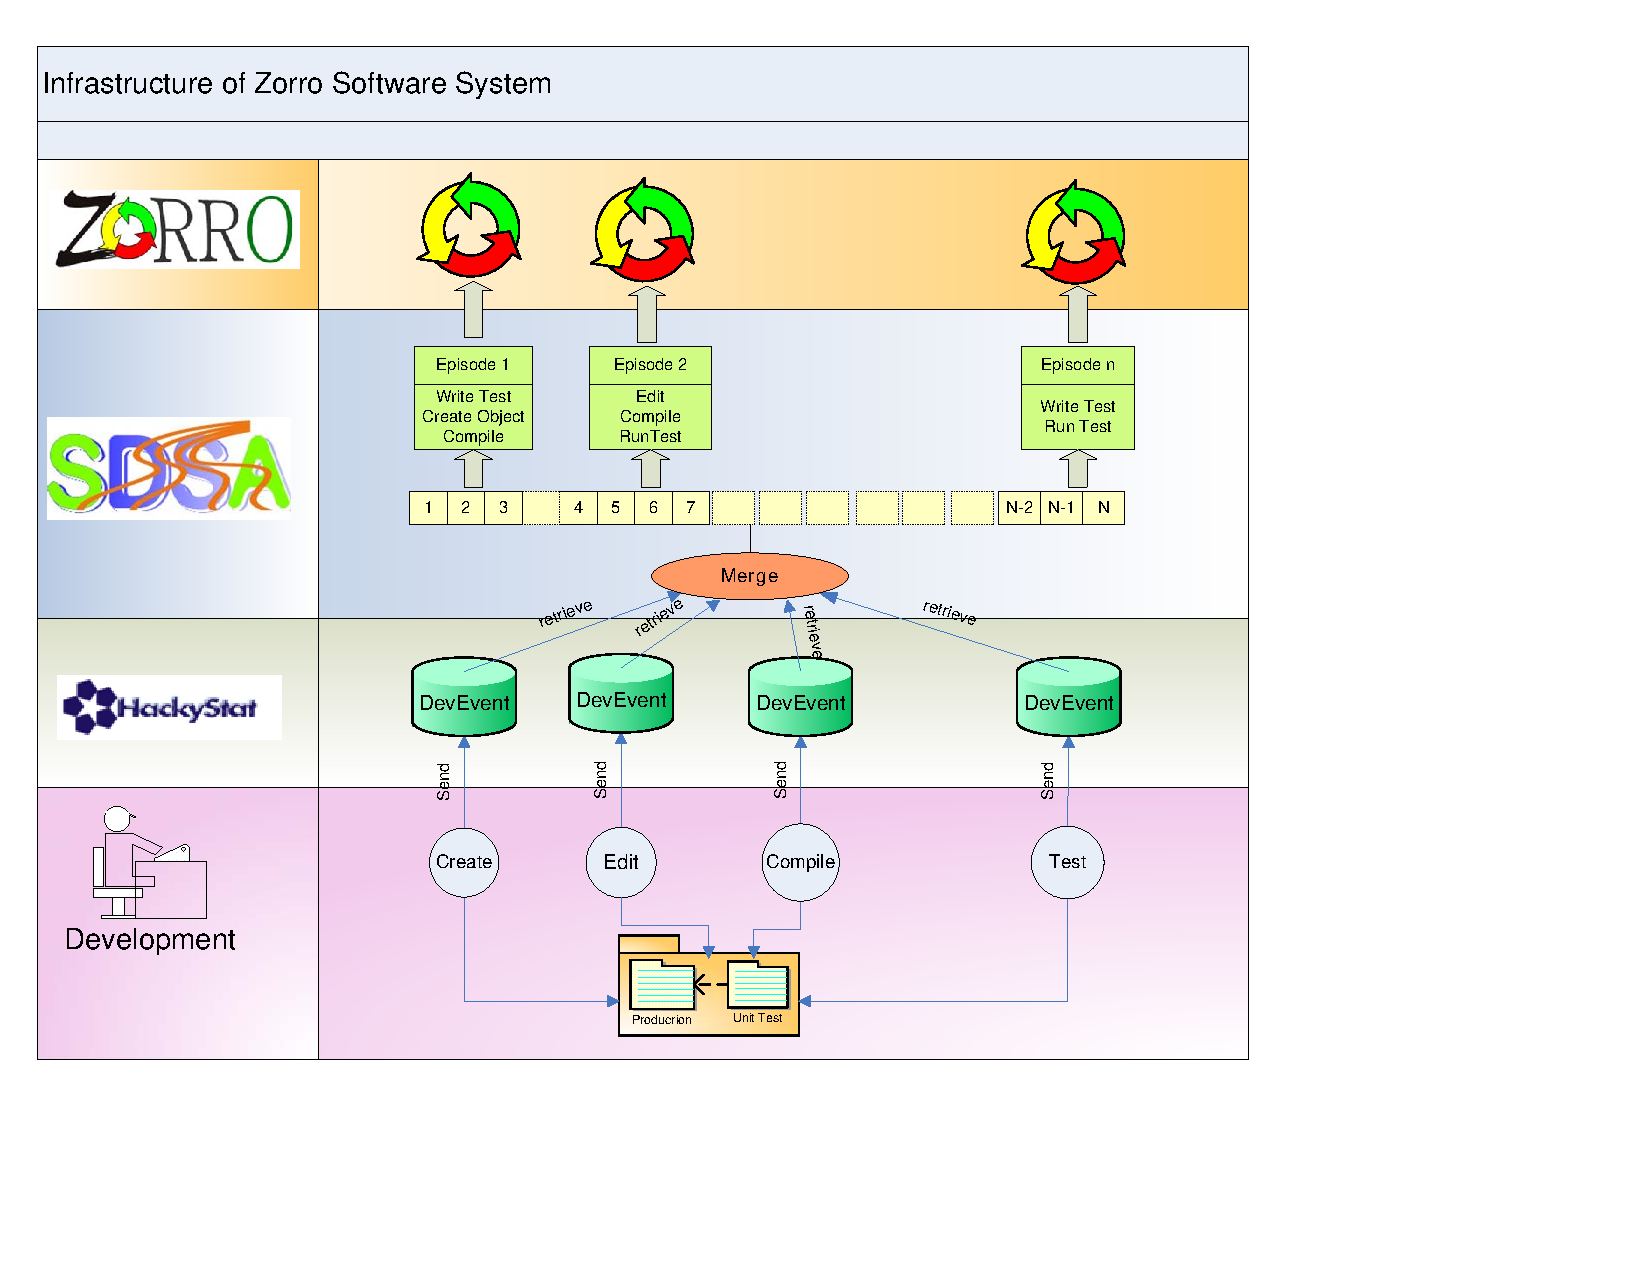
\includegraphics[width=1.0\textwidth]{figs/Visio-ZorroInfrastructure}
  \caption{Zorro Infrastructure}
  \label{fig:ZorroInfrastructure}
\end{figure}
In Figure \ref{fig:ZorroInfrastructure}, between Hackystat and Zorro layers, there is a middle tier named SDSA. The SDSA stands for the Software Development Stream Analysis, a generic framework for development event stream analysis including three components \textemdash software development stream construction, development stream partition, and development behavior inference. The SDSA is an extension of Hackystat, and it can be used to study low-level software processes.

\subsection{SDSA: A Framework of Development Stream Analysis}
The SDSA uses software metrics of development activities collected by Hackystat sensors to monitor, identify and characterize high-level development behaviors with the support of JESS \cite{Friedman-Hill:03}, a rule-based system in Java. Figure \ref{fig:Intro-SDSA-Workflow} illustrates the data models and work flow of SDSA. 
\begin{figure}[htbp]
  \centering
  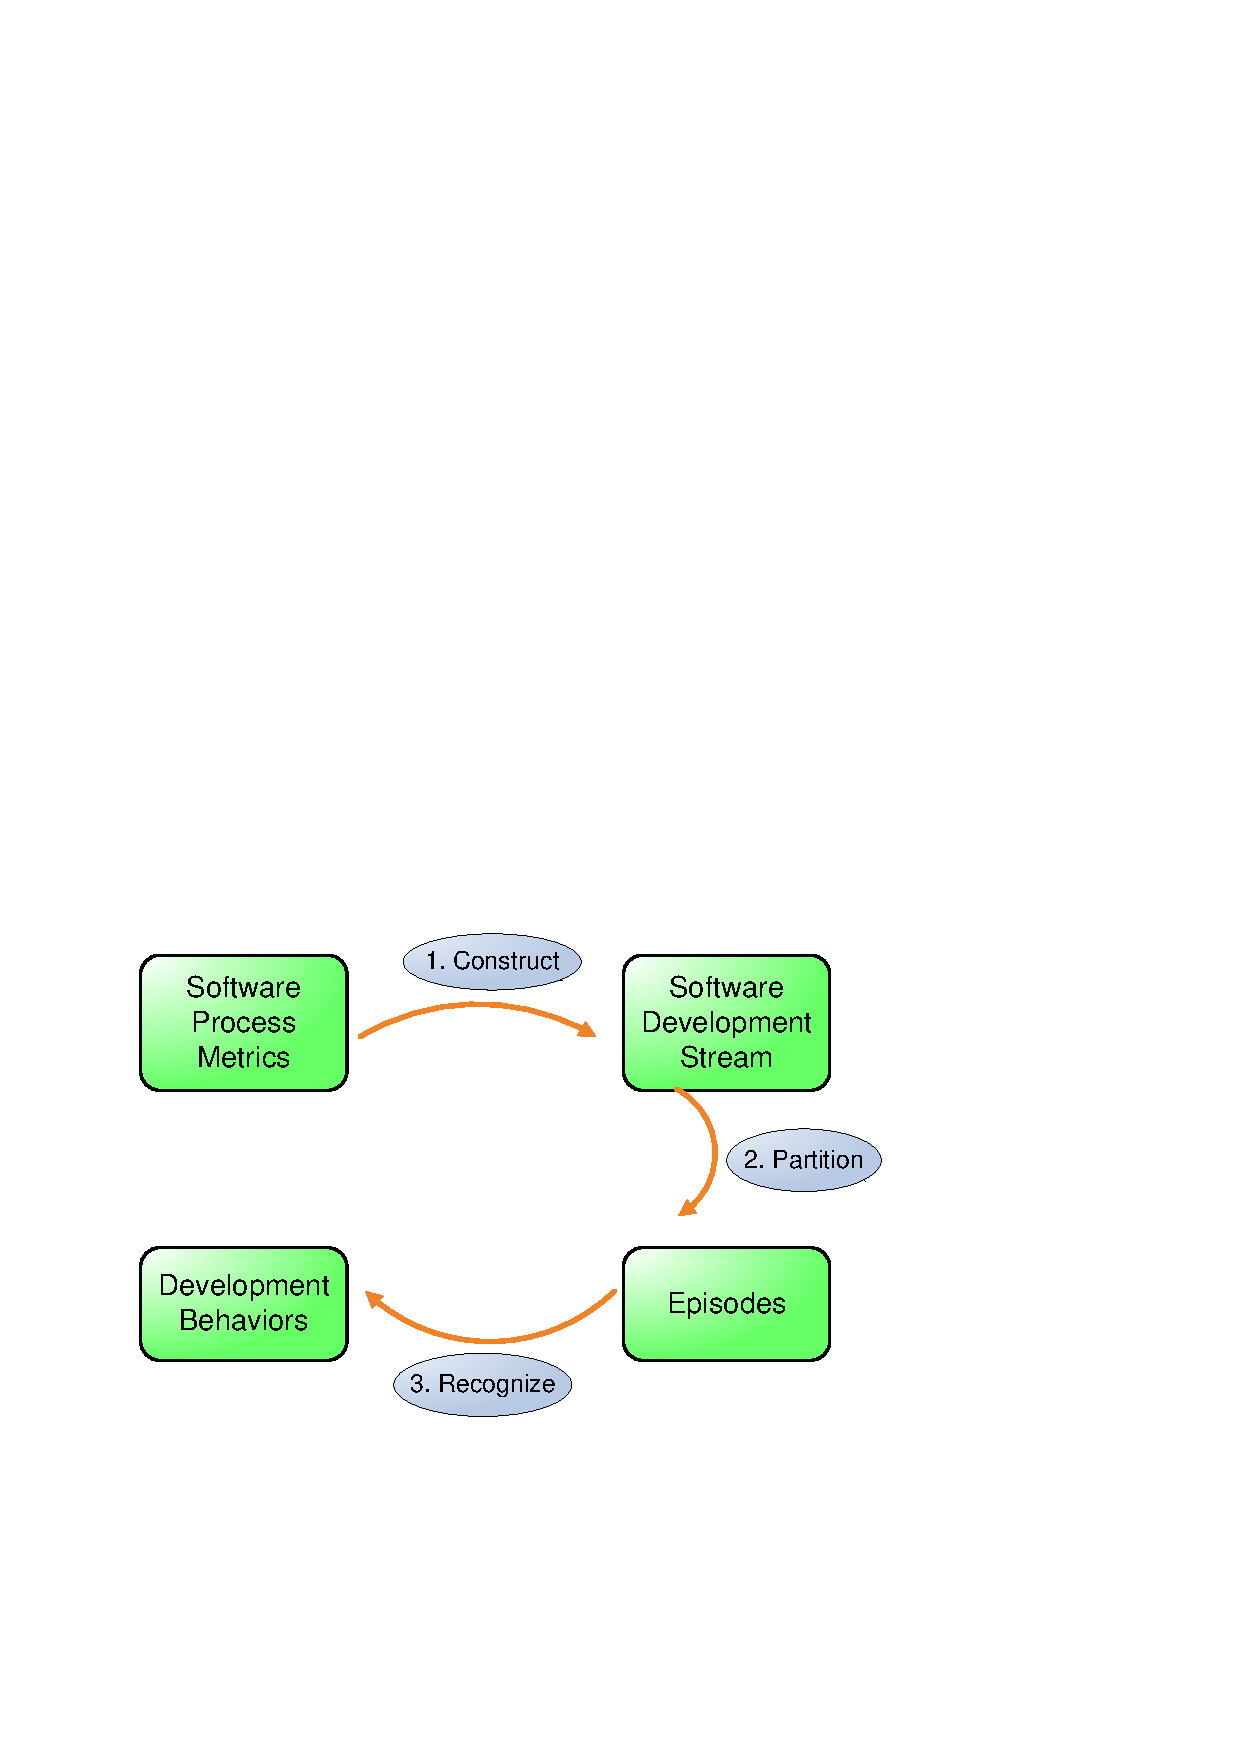
\includegraphics[width=0.5\textwidth]{figs/Visio-SDSA-FlowChart}
  \caption{SDSA Framework}
  \label{fig:Intro-SDSA-Workflow}
\end{figure}
The data models of SDSA include ``software development stream'', ``episode'', and ``development behavior''. A linear work flow connects software metrics and these three data models together in SDSA. First, SDSA processes the software metrics of development activities collected by Hackystat sensors. After reducing software process metrics into development activities, SDSA organizes development activities of a same type into a time-series event stream, which is a sub stream of the software development stream. SDSA assembles different event streams together to construct a ``software development stream'', which is also a time-series. Second, due to the complexity of digesting long development streams with heterogeneous development activities, SDSA uses a partition technique. A development stream can be partitioned into many episodes delimited by characteristic development activities. The episode is in turn a time-series collection of development activities. Third, SDSA includes a driver and interface to recognize the development behaviors in episodes using JESS. 

SDSA is tool and process independent. It can be instantiated to measure a software development method or low-level software process.

\subsection{Zorro Software System}
Zorro is an instantiation of the SDSA framework for TDD. It extends SDSA at three points: 
\begin{enumerate}
\item Development Stream Construction

As Figure \ref{fig:ZorroInfrastructure} illustrates, Hackystat sensors collect a variety of software metrics, and SDSA can construct a development stream with all of them. But this is not desirable because some development activities might not be relevant to the development method or process under study. Using TDD as an example, debugging is not interesting because it is not part of the process of TDD. In a nutshell, the essential development activities required by Zorro for TDD behavior inference are:
\begin{itemize}
\item editing activities including document, production and unit test editing,
\item buffer transition activities,
\item refactoring activities including addition, deletion, renaming, and moving of object components,     
\item unit testing activities,
\item compilation activities. 
\end{itemize}
Respectively, Zorro constructs the development streams of TDD with event streams including ``EditStream'', ``BuffTransStream'', ``RefactoringStream'', ``UnitTestStream'', and ``CompilationStream''.  

\item Tokenization

Zorro uses the ``test-pass'' tokenizer, which partitions the TDD development stream into a set of episodes that are delimited by successful unit test invocations. 

\item Development Behavior Recognition  

In Zorro, I defined a set of specific rules for TDD according to Beck \cite{Beck:01,Beck:03} and others who have described the practices of TDD. The ``test-pass'' episodes are categorized as ``test-first'', ``refactoring'', ``test-addition'', ``regression'', ``code-production'', ``test-last'', ``long'', or ``unknown''. Chapter \ref{ch:Zorro} has the detailed description of the episode classification schema. 

\end{enumerate}

After inferring development behaviors in episodes and categorizing them, Zorro uses the classification results as well as the context of episodes to reason the conformance of TDD. Figure \ref{fig:Zorro-Demo} is an excerpt of Zorro's TDD inference result for an experienced TDD developer. 
\begin{figure}[htbp]
  \centering
  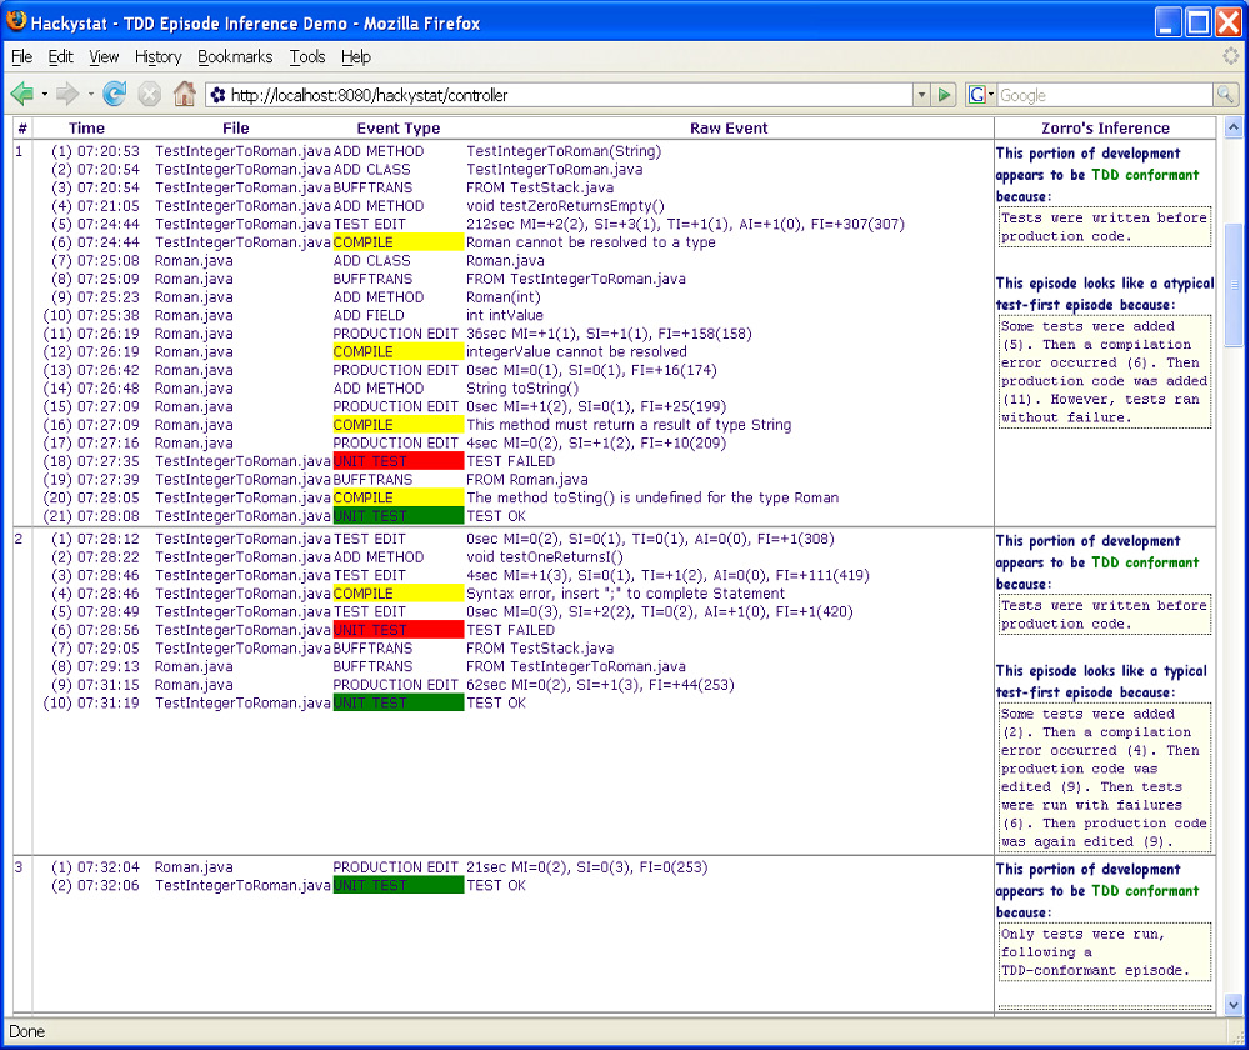
\includegraphics[width=1.0\textwidth]{figs/Zorro-Demo}
  \caption{Demo of Zorro's TDD Inference}
  \label{fig:Zorro-Demo}
\end{figure}
This experienced developer solved the Roman numeral conversion problem (Appendix \ref{app:UserStoriesRomanNumeral}) using TDD in the Eclipse IDE. The Hackystat Eclipse sensor was installed to instrument the development process to collect development activities. Zorro partitioned them into 16 episodes using the ``test-pass'' tokenizer, and inferred the process conformance of TDD.  In the table illustrated in Figure \ref{fig:Zorro-Demo}, the last column  contains the reasoning process and result. According to this table, the first three episodes are all TDD conformant. The first episode is ``test-first'' but atypical because production code was not edited to make test pass after the test invocation failed at (18). The second episode is ``test-first'' due to the perfect match of development activities to the red/green/refactor metaphor. The last episode is ``regression' because no progress was made although the production code was edited. Based upon the reasoned development behaviors and the context of episodes, Zorro inferred that all the three episodes are TDD compliant. 

With the automated software metrics collection and inference of TDD, a lot of useful analyses that once were thought impossible have become plausible. A handful of analyses (see Chapter \ref{ch:Zorro}) were implemented in Zorro. Figure \ref{fig:Zorro-Demography} illustrates one of them, the ``TDD Episode Demography'' analysis. 
\begin{figure}[htbp]
  \centering
  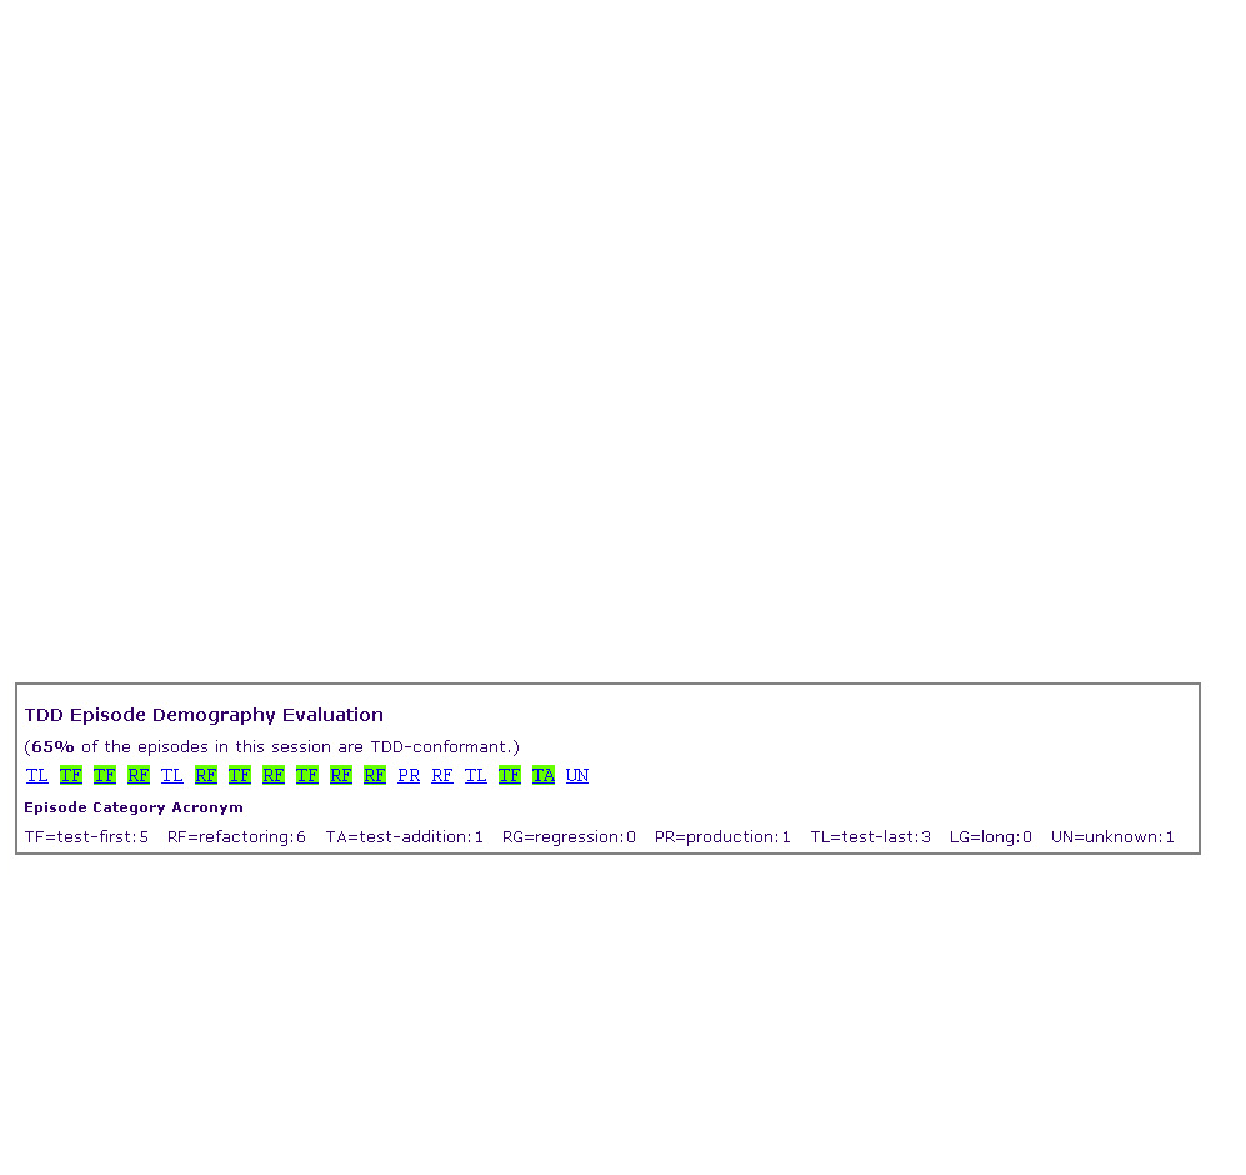
\includegraphics[width=1.0\textwidth]{figs/Zorro-DemographyAnalysis}
  \caption{TDD Episode Demography}
  \label{fig:Zorro-Demography}
\end{figure}
This analysis provides an overview of a TDD programming session, which is partitioned into 17 episodes, and 65\% of them are TDD compliant. Note that 
\begin{itemize}
\item each small box with a two-letter acronyms represents a single episode,
\item TDD-conformant episodes are shown in green. Non TDD-conformant episodes are transparent. 
\end{itemize}
For the TDD programming session illustrated in Figure \ref{fig:Zorro-Demography}, if Zorro was not used, the developer would falsely claim that he/she complied with TDD. In fact, as it turned out, the developer did not conform to the idealized TDD process all the time. According to Zorro's inference, 65\% percent of the episodes in this session are TDD-Conformant, and some episodes are ``test-last''. In addition to reporting the compliance of TDD, the ``TDD Episode Demography'' analysis can also be used to look for the development patterns. Episodes are ordered by time when they occurred. The researchers and developers can retrospectively review the development process for training or improvement. 

Besides typical analyses such as ``TDD Episode Demography'', I also implemented a group of telemetry analyses. The Software project telemetry \cite{csdl2-04-11,csdl2-06-05} was developed by Qin Zhang in the Collaborative Software Development Lab at the University of Hawaii. It can aggregate metrics data together to perform daily, weekly, or monthly analyses of the software metrics to support in-process software project management and decision makings. 
 
Some goals of this dissertation research are to assist the education, training, improvement, and empirical evaluations of TDD. Software project telemetry is an infrastructure that can be used by Zorro to pursue these goals. In Zorro, I have already defined telemetry streams including ``TDD percent of development time'', ``TDD percent of episodes'', ``development time ratio of test and production code'', ``size ratio of test and production code'', and so forth. Figure \ref{fig:Zorro-TDD-Coverage} is a weekly telemetry chart showing percentage of TDD development and test coverage.
\begin{figure}[htbp]
  \centering
  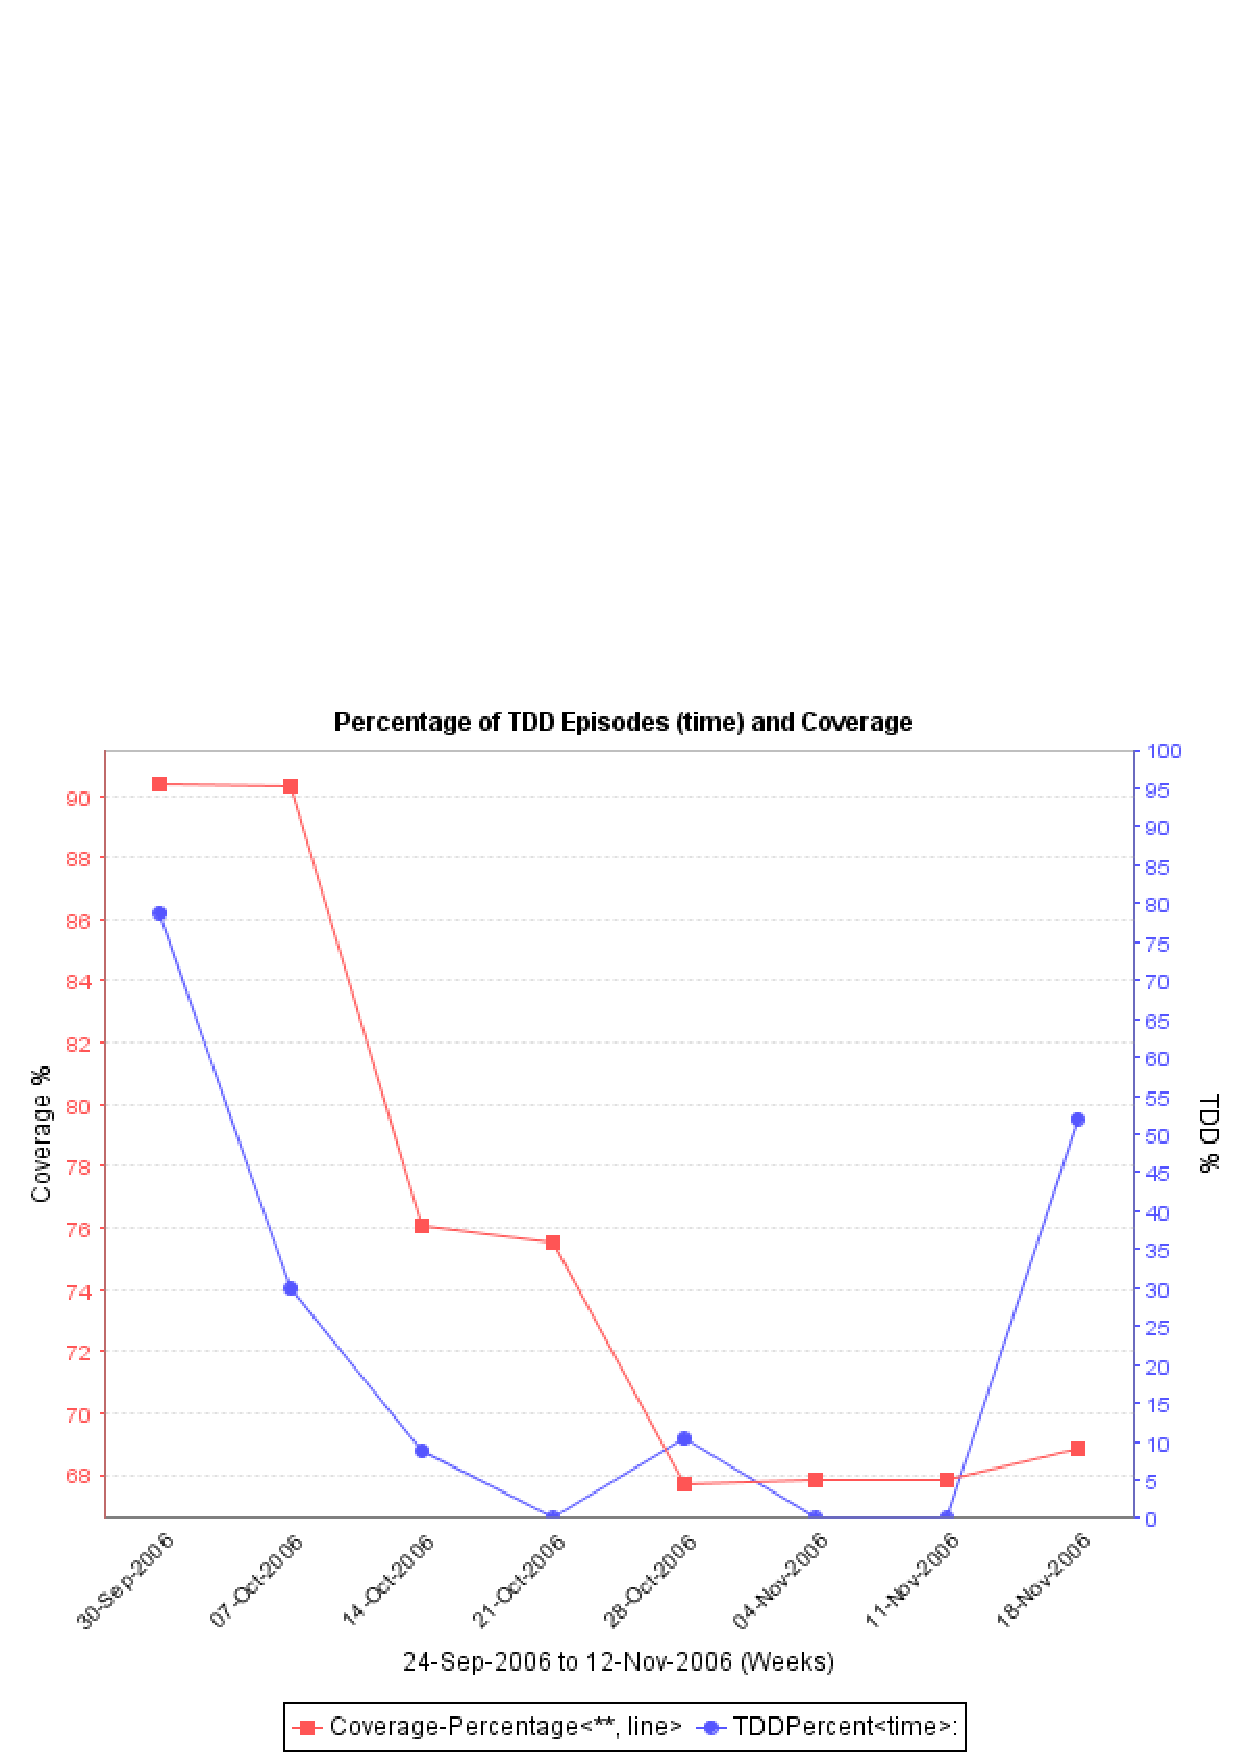
\includegraphics[width=1.0\textwidth]{figs/Zorro-TDD-Coverage}
  \caption{Proportion of TDD vs Test Coverage}
  \label{fig:Zorro-TDD-Coverage}
\end{figure}
From the week of Sep 30, 2006 to the week of Nov 18, 2006, I worked on the Zorro software system and implemented Zorro's web validation interface. I used TDD in my development. Due to the fact that testing web interfaces requires a lot of additional effort, my percent of TDD development dropped down significantly in that period. As a result, the test coverage of Zorro dropped from above 90\% to below 70\% over the course of eight weeks software development. 

The synergy of Zorro and telemetry allows practitioners and researchers to improve the practice and research of TDD with no additional overhead. Both systems are automated based on Hackystat's automatic software metrics collection with sensors attached to the development environment tools. 

\section{Research Statement}
In this dissertation, I created the Zorro software system to study the conformance of Test-Driven Development in practice with the aids of the Hackystat framework and the Software Development Stream Analysis (SDSA) framework that I have developed. The design of the Zorro software system is a combination of bottom-up and top-down methods. The development environment tools are instrumented by Hackystat sensors to collect software process and product metrics. A variety of software metrics are abstracted into development activities and then are merged together to form the time-series software development stream, which is then partitioned into small chunks named ``episode''. This portion is bottom-up. Given a software development method or low-level software process, the process description, guideline, and knowledge can be translated into a set of rules. The rules can be used to evaluate episodes partitioned from the software development stream. This portion is top-down.

The success of Zorro relies on the software metrics collection capability as well as the comprehension of TDD. The software metrics that are related to TDD must be collected. In the long run, it is important for the software development community to reach some kind of consensus on an appropriate definition (or definitions) for TDD. Until there is concrete experience from Zorro, this consensus is not feasible. The development of Zorro is thus iterative and progressive. Figure \ref{fig:Zorro-Timeline} illustrates the time line of this research project including a few milestones. 
\begin{figure}[htbp]
  \centering
  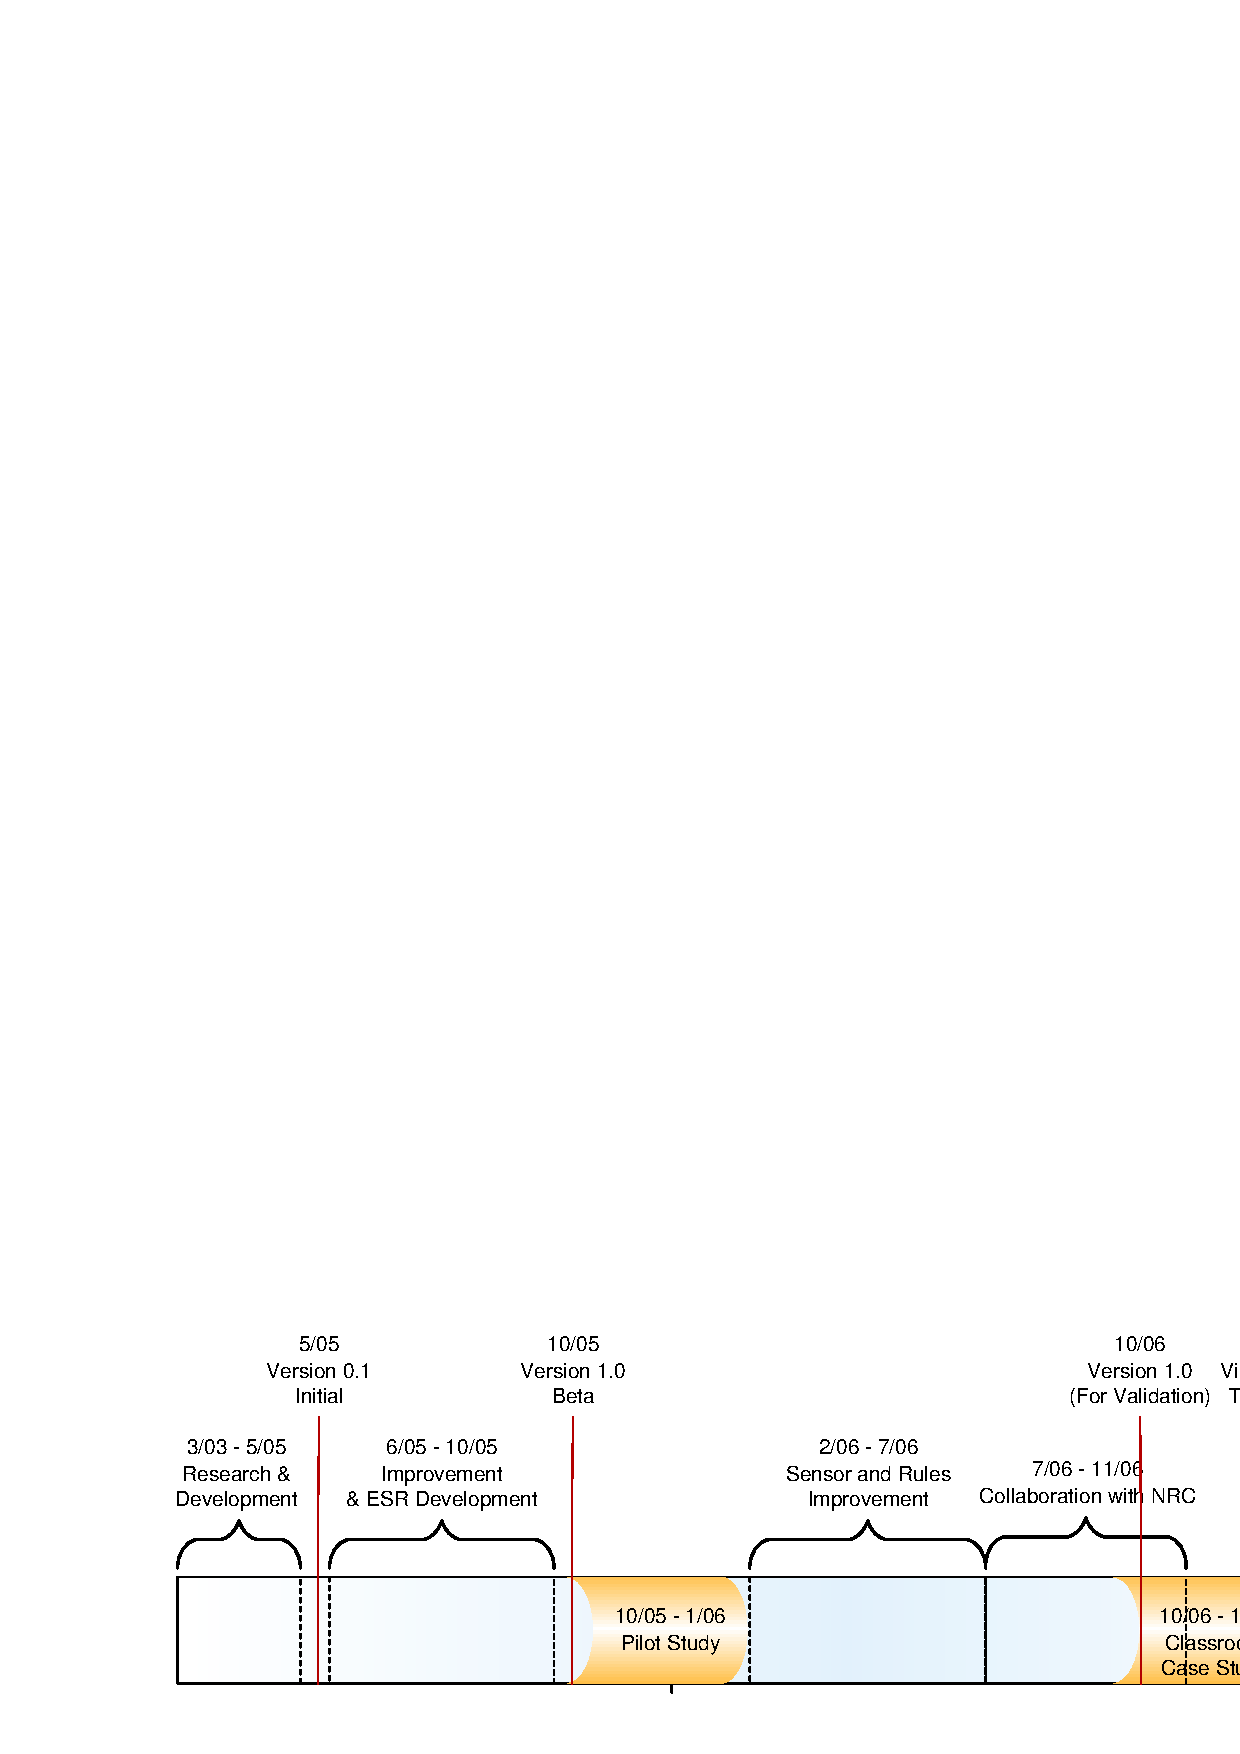
\includegraphics[width=1.0\textwidth]{figs/Visio-Zorro-TimeLine}
  \caption{Development Timeline of the Zorro Software System}
  \label{fig:Zorro-Timeline}
\end{figure}
I have conducted three empirical evaluations in my development process of Zorro to investigate whether Zorro can collect enough software metrics and how well it can infer TDD compliance. The Eclipse Screen Recorder (ESR, \cite{esr}), an Eclipse plug-in that can record development activities in the Eclipse IDE, was developed to assist the evaluations. ESR can capture Eclipse screen at the rate of 1 frame per second, and thus it provides high fidelity movies for the purpose of validation. The last empirical case study was conducted off-site in Norway to investigate what values Zorro can provide for researchers and project managers. 

\section{Empirical Evaluations}
\label{sec:introduction-evaluation}
Three longitudinal case studies --- a pilot study, a classroom case study, and an industrial case study were conducted to empirically validate the Zorro software system in this dissertation research. The primary goal of these studies was to validate Zorro's software metrics collection as well as TDD inference abilities. The secondary goal was to investigate how useful Zorro would be. An additional goal was to investigate how the metrics collection and inference rules can be improved. 

\begin{comment}
The software development processes in both studies were instrumented by the Eclipse Screen Recorder (ESR) \cite{esr}, an Eclipse plug-in that can record the software development process in the Eclipse IDE. The videos recorded by ESR were analyzed to validate Zorro's data collection and TDD inference. 

The goal of the first two studies was to evaluate and improve Zorro's software metrics collection and TDD inference capability in academic settings. 

tune the sensor and inference rules. The industrial case study was an attempt to deploy Zorro in the real TDD development situations. The primary goal was to explore how Zorro can assist project managers and researchers gaining insights of TDD.
\end{comment}

\subsection{Pilot Study}
After researching related work on TDD and stream analysis techniques, I designed and implemented the Zorro software system based upon my observation and analysis of TDD development patterns. By the Spring 2005, I had solved all the difficulties of metrics collection in the Eclipse IDE as a pilot, implemented the SDSA framework, and developed the first set of TDD recognition rules. 

I refined the initial version of Zorro in the Summer 2005, and conducted a pilot validation study in the Fall 2005. Six experienced Java programmers participated in this study. Each participant developed a implementation of the stack data structure (Appendix \ref{app:PilotStudyMaterial}) using TDD in the Eclipse IDE, which was instrumented by the Hackystat Eclipse sensor. I compared Zorro's inference to an independently collected source regarding their development behaviors. 

One approach to independent data collection would be to have an observer watching developers as they programmed, taking notes as to what development behavior they are conducting and whether they are pertaining to TDD or not. I considered this but discarded it as unworkable: given the rapidity of development activities in TDD, it would be very hard for an observer to notate all of the TDD-related development activities that can occur literally within seconds of each other. Therefore, I took another approach by developing the Eclipse Screen Recorder \cite{esr}. The ESR generates a QuickTime movie containing time-stamped screen shots of the Eclipse Window at the regular intervals. One frame/second was found to be sufficient for validation, generating file sizes of approximately 7-8 MB per hour of video. The QuickTime movie created by ESR provides a visual record of development behaviors that can be manually compared to the Zorro analysis using the timestamps for validation purpose. Figure \ref{fig:ESR-Video} is a screen copy showing the recorded development process movie played in the QuickTime Pro software \cite{QuickTime}.
\begin{figure}[htbp]
  \centering
  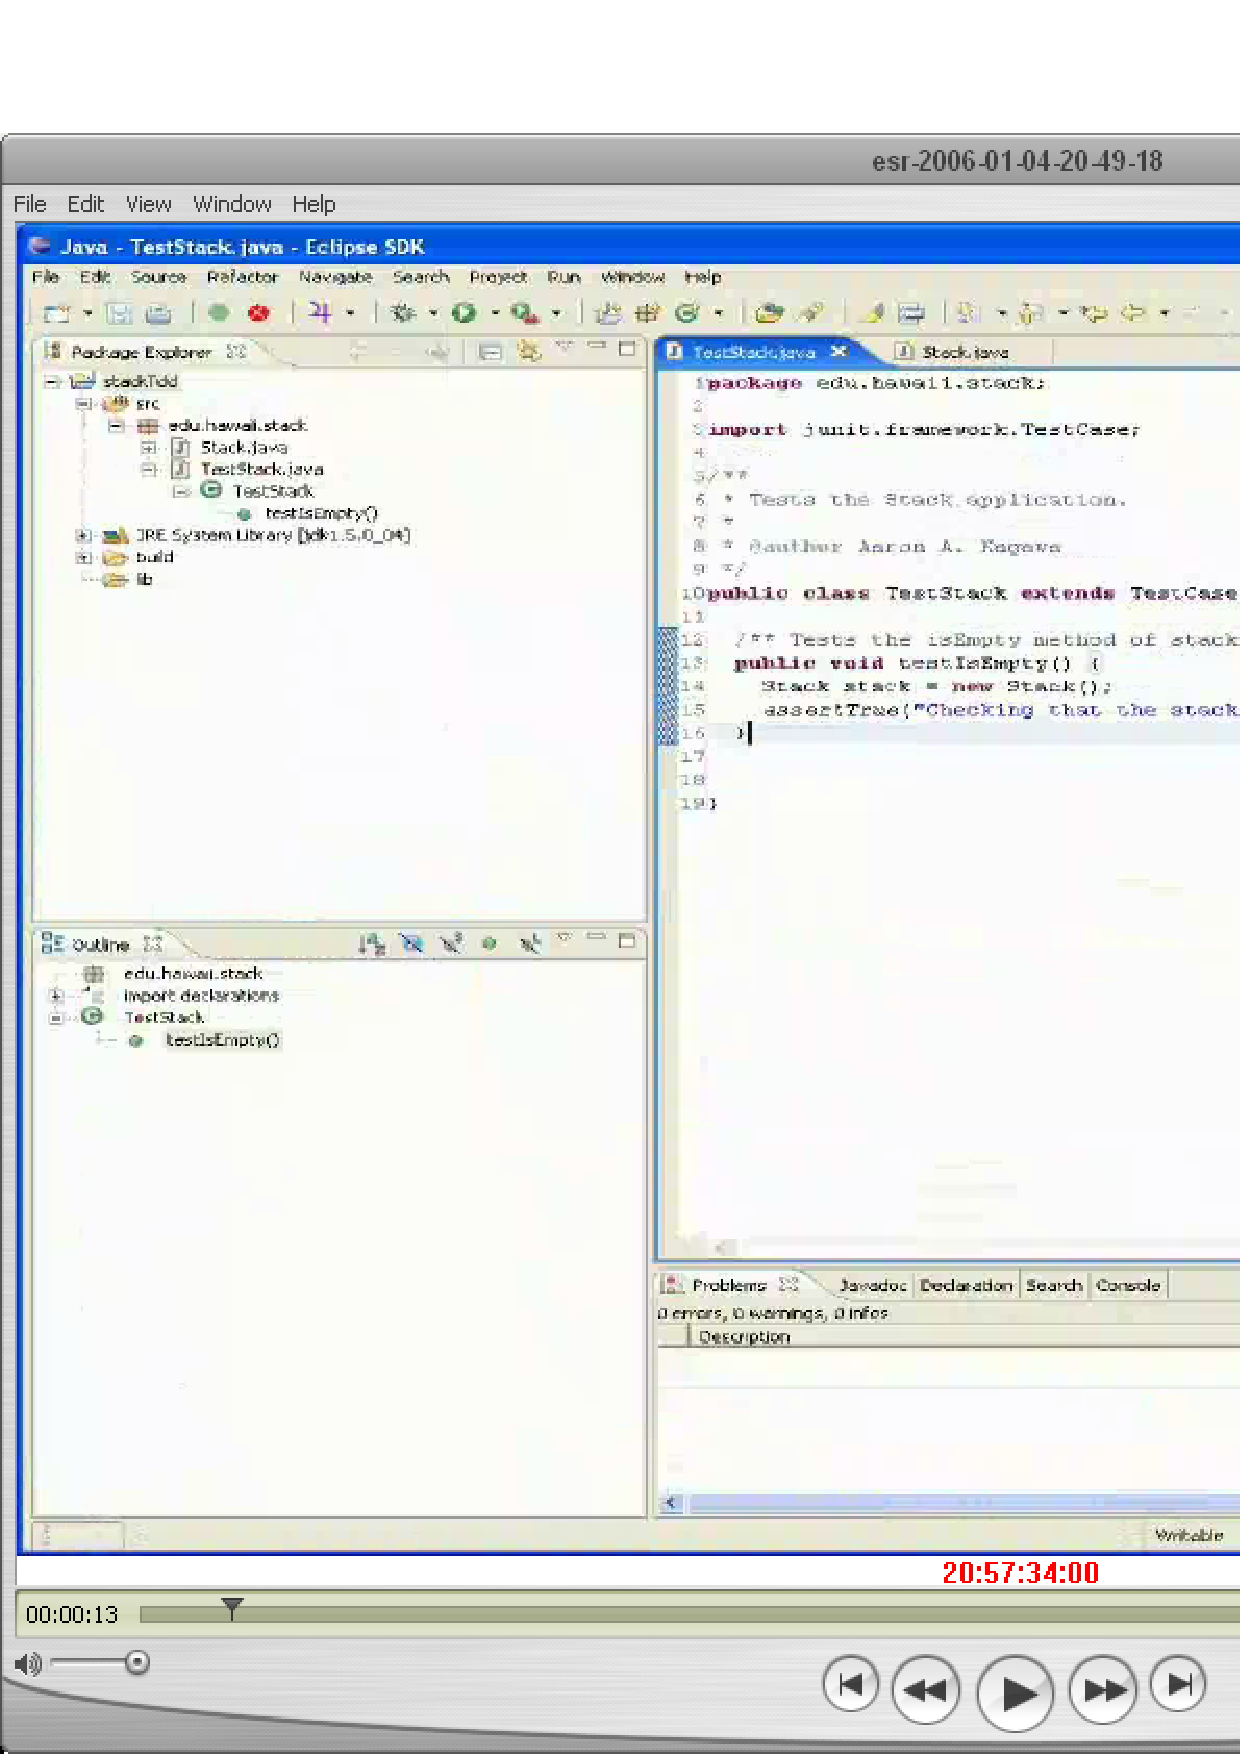
\includegraphics[width=1.0\textwidth]{figs/ESR-Video}
  \caption{Analysis of QuickTime Video}
  \label{fig:ESR-Video}
\end{figure}

The participants spent 28 to 66 minutes on the programming task. Zorro partitioned the overall development efforts into 92 episodes, out of which 86 were classifiable; 6 were unclassifiable. It classified 76 out of 86 episodes correctly resulting in classification accuracy rate 88.4\%.

The pilot study showed that Zorro is promising at inferring high-level development behaviors with low-level development activities collected as software metrics at least in a simple environment setting. The pilot study also showed that the metrics collection missed some information that led to inference errors. 

In the Spring 2006, I improved the Hackystat Eclipse sensor for metrics collection, and refactored Zorro's inference rules. In the Summer 2006, under the suggestion of Dr. Philip Johnson, I went to National Research Council of Canada (C-NRC), where I collaborated with Dr. Hakan Erdogmus, a senior agile process researcher who pioneered the idea of automated TDD conformance inference. The collaborative research at the C-NRC and the follow-up collaboration in the Fall 2006 resulted in a classroom case study and an industrial case study in the Spring 2007. 

\subsection{Classroom Case Study}
I, the author of Zorro, compared the recorded movies with Zorro's inference to validate Zorro's metrics collection and TDD development inference in the pilot study. I could be biased both at judging what software metrics are necessary, as well as at inferring development behaviors from the observed activities in the ESR movies. One man's subjective judgment, especially the one from author himself or herself, perhaps is not a valid measure in a case study \cite{Yin:03}. This is notably called ``construct validity'' problem according to \cite{Yin:03}. Using multiple data sources, establishing the chain of evidence, and having key informants review draft case study report are three viable tactics that a researcher can use to avoid the construct validity problem. Thus, in the Fall 2006, I developed a web interface to collect participant's comments, the third data source. 

In the Fall 2006, I conducted the classroom case study in the software engineering classes at the University of Hawaii. The  experimental design of this study is very close to the pilot study. Participants also developed using TDD in the Eclipse IDE with the instrumentations of the Hackystat Eclipse sensor and ESR. The differences were that the Hackystat Eclipse sensor was more robust and the new problem (Bowling Score Keeper at Appendix \ref{app:UserStoriesBSK}) was much harder than the stack data structure (Appendix \ref{app:PilotStudyMaterial}). 

Eleven students from the software engineering classes voluntarily participated in this study. The participants developed in TDD for 90 minutes, followed by a 10 minute interview and a 20 minutes Zorro inference validation session. In the interview, I asked them questions regarding their opinions on unit testing and Test-Driven Development. A digital voice recorder was used in the interview and in the following validation session for their verbal comments.

The classroom case study data analysis supported the claim that  Zorro's metrics collection is as good as ESR, if it is not better. Zorro's TDD compliance inference has two steps. It infers development behaviors in episode first, and then uses the inferred results and context to reason the conformance of TDD. The video analysis validated that Zorro inferred episode development behaviors with 70.1\% accuracy and TDD compliance with 89.1\% accuracy. The third data source, cross-validation with participant comments, is only slightly different from my video observation analysis. 

The participant interview analysis suggested that unit testing is good at yielding high quality software but majority of participants (7 out of 10) admitted that they did not test enough. Perhaps TDD should be used to improve both developers' confidence and software quality. The data analysis also suggested that TDD is hard to do although half of participants like to develop software using TDD in the future. Therefore, providing a tool such as Zorro to assist practice of TDD has the potential to help beginners. The usefulness evaluation conducted in this study suggested that some of Zorro's TDD analyses are useful for this purpose. 

\subsection{Industrial Case Study}
On one hand, I planned the classroom case study for an extended validation after the pilot study. On another hand, I worked with Dr. Philip Johnson and Dr. Hakan Erdogmus to solicit the collaboration with other researchers and practitioners who are also interested in empirical study of TDD. The Zorro demo \cite{ZorroDemo:06} was developed to demonstrate how Zorro works and what analyses it provides. This effort led to collaboration with Dr. Geir Hanssen and Dr. Tor Erlend F{\ae}gri from SINTEF ICT of Norway. They are performing research on the effectiveness of TDD, in contrast to Test-Last Development, the opposite side of TDD. They found that collecting the information about TDD is very hard and Zorro has the potential to provide higher quality information about TDD.

A European software company that provides a packaged software product for marketing and customer surveys \cite{Hanssen:06} is the participant of this industrial case study. However, the development tool is Visual Studio .NET Team Edition and the programming language is C\#. We rapidly developed a Zorro compatible Visual Studio sensor for this industrial case study. A Hackystat server is installed on a Windows 2000 server provided by the company. I remotely managed the server for this industrial case study. Out of 20 participants, 12 were in the TDD project and the remaining 8 were in the non-TDD project. Unfortunately, the participation in this study was very low. As to my report written at the end of March 2007, 25\% of developers installed the sensor and collected development data,  25\% of developers installed the sensor but did not update it as requested, 25\% of developers installed the sensor but the sensor did not send any data to the server after a pilot, and the rest 25\% of developers did not install the sensor according to my 
observation of the Hackystat server status. The project manager indicated that Zorro's inferred development behaviors did not agree with what developers actually did, but provided no detailed information. It turned out that it is much harder to have industry participants install the sensor, and it is also hard to relate collected data to actual development behaviors, particularly if the study had to be conducted remotely. However, Dr. Geir Hanssen and Tor Erlend F{\ae}gri have expressed interests to continue using Zorro in the future studies. This case study served as a pilot test only.  

\section{Contributions}

My contributions include the SDSA framework, the Zorro software system, and the systematic empirical evaluation of Zorro:
\begin{enumerate}
\item \textbf{SDSA Framework}

The Software development is a very complicated process including a series of continuous development activities, yet not independent of each other. The SDSA framework abstracts continuous, interwoven development activities collected by Hackystat sensors in a programming session into a software development stream. The software development stream is a linear, time-series data structure. 

A development stream can be partitioned by SDSA using tokenizers into episodes, another abstract data type representing a micro-iteration of a software process. Tokenizers are expandable and selectable. A different set of tokenizers can be applied according to the studied software process.

The SDSA framework characterizes development behaviors in episodes using JESS, a rule-based system in Java. A classifier interface is provided in SDSA to flexibly supply inference rules. Moreover, the rules can be changed on the fly. 

In my thesis research, I instantiated the SDSA framework on Test-Driven Development (TDD), and the system resulting from this work is the Zorro software system that can automatically infer the development behaviors and the compliance of TDD. This research work demonstrated that the SDSA framework has the potential to be useful for researching other low-level software processes. 

\item \textbf{Automated Recognition of TDD with Zorro}

Zorro recognizes TDD automatically with the software metrics collected by Hackystat sensors in the IDEs. The contributions of Zorro's implementation include the enhanced Eclipse and Visual Studio .NET sensors, a suite of TDD recognition rules, and many useful analyses for understanding TDD in practice.

The Eclipse and Visual Studio .NET Team Edition are two IDEs that are Zorro compatible. The sensors of these two IDEs collect a variety of process metrics such as editing, refactoring, testing, compilation, and so on. Many useful product metrics such as methods, statements, test cases, and assertions are collected too. The progressive changes of software product metrics are very useful information for software engineering research.

The recognition rules are from the descriptions of many well-known TDD practitioners including Beck \cite{Beck:03}, Doshi \cite{TDDQuickReference}, and Erdogmus, and my grounded observation of TDD in practice. 

Many analyses were developed to display Zorro's inference processes and results, report different aspects of TDD such as episode duration distribution. The TDD telemetry streams were developed to support the in-process decision makings for software project management.  

\item \textbf{Empirical Evaluations}

My contribution to the empirical evaluations are:
\begin{enumerate}
\item ESR \cite{esr}, a software system that can record Eclipse usage; 
\item The availability of the Zorro software system for use by other researchers under an open source license;

\item The experimental method exemplified by the case studies, which shows how to conduct research on TDD that does not suffer from the process conformance problem;

\item The actual results of the case studies, which show (i) the Zorro can identify TDD, that (ii) users found Zorro analyses to be useful in certain cases and not in others, and (iii) that industrial case studies on TDD are more difficult than classroom case studies, as it is more difficult to get developers to install sensors, and more difficult to relate data back to their development.

\end{enumerate}
\end{enumerate}

\section{Dissertation Structure}

This thesis is organized into the following chapters. 

\begin{itemize}
\item Chapter 1 introduces the TDD challenges and the motivation of this research. 
\item Chapter 2 presents the related research work. 
\item Chapter 3 describes the SDSA framework in details.
\item Chapter 4 describes the Zorro software system in details.
\item Chapter 5 briefs the research questions and methodology of this dissertation. 
\item Chapter 6 reports the pilot study data analysis in details.  
\item Chapter 7 reports the classroom case study data analysis in details.
\item Chapter 8 reports the industrial case study conducted off-site.
\item Chapter 9 synthesizes the results from the empirical case studies, presents
the conclusions of this research, and discusses the future work.
\end{itemize}

\begin{comment}

The software development is a highly cognitive process in which developers continuously interact with development environment tools to produce the software artifacts following a certain process. 

Software metrics are great assets out of research work in the software engineering discipline. The typical use of software metrics is through the Goal-Question-Metric (GQM) paradigm where the software metrics are used as the measure to high-level questions and goals.  A significant drawback of the GQM is that software metrics are not always possible to be collected, or can be collect in high cost. 
\end{comment}

%%%%%%%%%%%%%%%%%%%%%%%%%%%%%%%%%%%%%%%%%%%%%%%%%%%%%%%%%%%%%%%%%%%%%%%%%%%%
%% Start of the old introduction
\begin{comment}
Throughout the history of software engineering, much effort has been put on the description and understanding of high-level software processes. The waterfall model, the very first software process, has contributed to the success of many large software systems. High-level software processes divide the software development process into phases, where each phase lasts from a few days to several months \cite{Pfleeger:01,Pressman:03}. For example, the requirements analysis phase may last months before the design phase starts. Recently, increasing effort has been put on low-level software processes \cite{Larman:03,AgileAlliance}, in which a phase may last several minutes to a few hours only. Each phase defines how developers and development team should carry on the work on daily basis. The Personal Software Process (PSP) \cite{Humphrey:99} and Extreme Programming (XP) \cite{Jeffries:00,Beck:00,XP96} are two examples of a low-level software process. Although proven to be useful in improving software quality\cite{Ferguson:97,Kamatar:00,MicrosoftTSP,Janzen:05}, low-level software process are hard to execute correctly and repeatedly. In order to improve the quality of practice and research of low-level software process, there must be some supporting tools. In my dissertation research, I focus on one low-level software process, the called Test-Driven Development (TDD) \cite{Beck:03}, and I developed Zorro software system to study it.

Test-Driven Development (TDD) is an innovative one of the practices of Extreme Programming. In TDD, the software development process is iterative and incremental \cite{Larman:03}. There is only one task to accomplish in an iteration. In a particular iteration, a unit test of the task is created first followed by production code implementation.  TDD is built on the foundation of the XUnit framework \cite{XUnit}, which has been ported to more than 30 languages. Unit testing has become a de facto standard in the software industry. TDD is widely adopted by software professionals. An informal survey \cite{UnitTestingPoll:06} conducted by Method and Survey magazine found that 46\% of the studied software organizations perform unit testing informally, 41\% of the studied organizations document their unit test cases, and 14\% of the studied organizations use the TDD approach.

``Clean code that works''\cite{Beck:03} is the goal of Test-Driven Development. To achieve this goal, TDD summarizes its software development process as two basic rules: ``(1) Write new code only if an automated test has failed; (2) Eliminate duplication.''  Kent Beck, the pioneer of Test-Driven Development, stated that there is an implicit order to software development using TDD \cite{Beck:03}: 
\begin{enumerate}
\item Red - Write a little test that does not work, and perhaps does not even
  compile at first.
\item Green - Make the test work quickly, committing whatever sins are
  necessary in the process.  
\item Refactor - Eliminate all the duplication created by merely getting
  the test to work.  
\end{enumerate}
At first glimpse, TDD seems easy, but in fact, it is a very hard and difficult low-level software process that requires much discipline to carry out correctly. First, software developers are not typically educated to write unit tests for the program they develop. Therefore, in a lot of cases, software systems are not designed for easy testing. Consequently, developers often find it is hard for them to write testing code at all, much less write testing code prior to implementation. Second, following the red/green/refactor software development pattern requires a lot of effort. In TDD, software developers must continuously remain in the mindset of test-first, which is initially counter-intuitive to many of them \cite{Beck:01,Wang:04}. So they often apply it differently according to their own experience level and understanding \cite{Beck:01}.

TDD is gradually becoming a standard well accepted for software development in industry, and yet there are problems in testability and differences in understanding of this methodology. Not surprisingly, the immaturity of TDD causes problems. There are many important research questions regarding software development using TDD. For example, how do we know software developers will faithfully commit to the highly disciplined TDD practice? Will developers slip away from TDD? When does it pay off to use TDD, and when does it not pay off? One thing is clear: these questions cannot be answered accurately without good software process measurement. However, Janzen and Saiedian \cite{Janzen:05} stated that measuring the use of a software development methodology is hard. They claimed it is so hard to do accurately that published data on the level of TDD adoption in industry is either indirect or inaccurate \cite{Janzen:05,UnitTestingPoll:06}.  Fortunately, as my initial case study demonstrates, measuring the use of certain software development methods is becoming feasible with the emergence of technologies such as the Hackystat system \cite{Hackystat:06,csdl2-04-11,csdl2-04-22,csdl2-03-12}, an in-process software metrics collection and analysis framework.

As part of my dissertation research, I developed a software system called Zorro (Figure \ref{fig:ZorroInfrastructure}) on top of Hackystat to infer TDD development behaviors using low-level software development activity data collected by Hackystat Eclipse Sensor.  Zorro recognizes and evaluates TDD patterns using rule-based system support and the software development stream analysis (SDSA) framework. SDSA is a three-stage analysis technique that brings the Hackystat framework and Zorro system together. First, it merges software development activities and in-process metric data together to create a ``software development stream'', a sequential stream of low-level software development activities. Second, SDSA includes a tokenization subsystem that divides a single sequential stream of low-level software development activities into collections of events called ``software development episodes''. Third, the JESS \cite{Friedman-Hill:03} rule-based system recognizes and classifies these episodes according to the classification schema.  SDSA binds these three components together to assist the measurement of software development methods and low-level software process.
\begin{figure}[htbp]
  \centering
  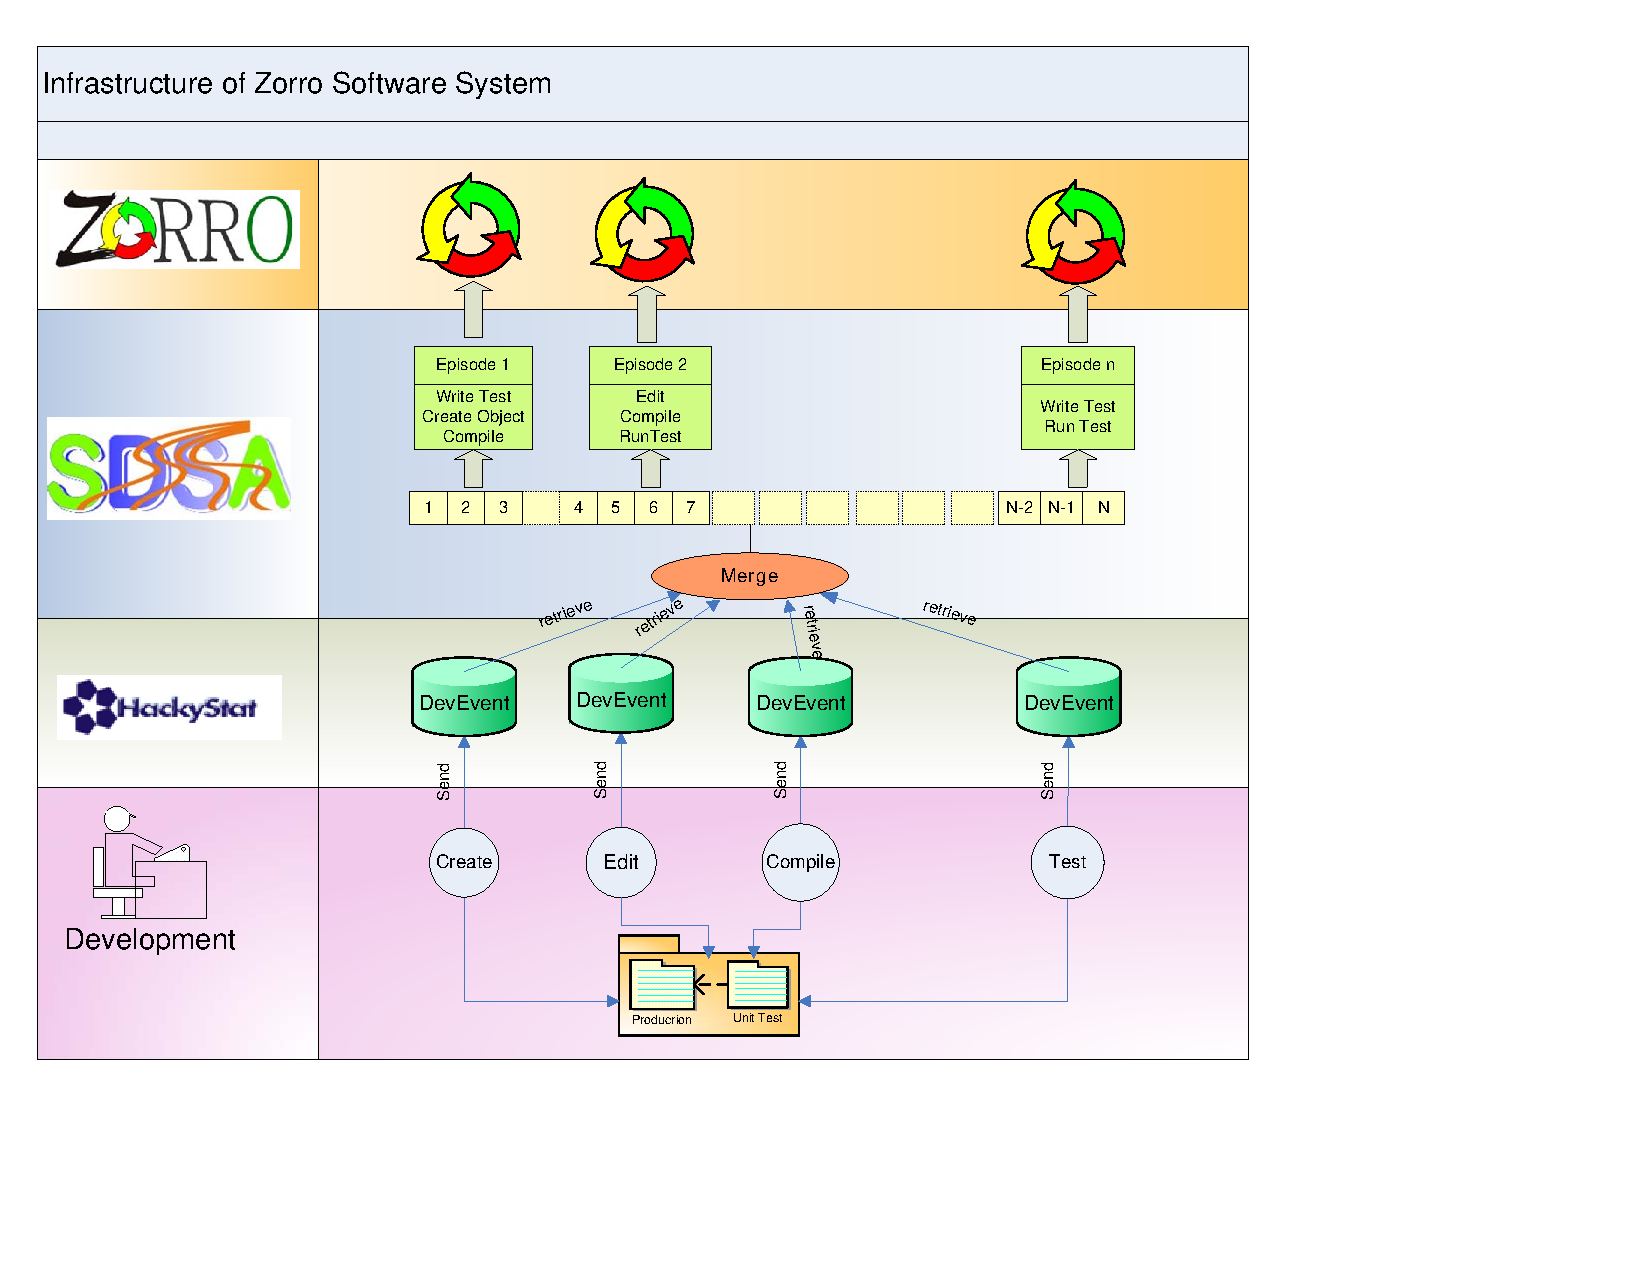
\includegraphics[width=0.9\textwidth]{figs/Visio-ZorroInfrastructure}
  \caption{Zorro Infrastructure}
  \label{fig:ZorroInfrastructure}
\end{figure}

With the capabilities provided by SDSA, I defined a set of specific rules for TDD in Zorro according to Beck \cite{Beck:01,Beck:03} and others who have described the practices of TDD. Zorro uses a two-step procedure to measure and evaluate the compliance of the developer's behaviors with the practices of TDD.  First, Zorro recognizes and classifies the episodes independently according to the classification schema. Second, Zorro evaluates the internal structure as well as the context of the episodes to deduce whether an episode is TDD conformant or not.
\end{comment}
\chapter{Related Work}
\label{ch:RelatedWork}

Test-Driven Development (TDD), a core practice of Extreme Programming, 
has been widely adopted by software industry and studied by software 
engineering researchers. Industry practitioners have put increasing 
effort into evaluating and understanding TDD in recent years. Many books \cite{Beck:03,Astels:03,Newkirk:04,Link:03,Hunt:03} directly related 
to TDD have been published. XUnit\cite{XUnit,xUnitFrameWork}, the 
foundation of TDD, has been ported to more than 30 languages. Development 
tools such as Eclipse, NetBeans, and Visual Studio have been enhanced
to support unit testing, which makes it easier for practitioners 
to develop software in TDD. The community of TDD \cite{TestDrivenWeb,TddYahooGroup} 
is continuously growing, and some enthusiastic practitioners 
\cite{HawleyBlog,ExtremeJSBlog,MemoRandaBlog,EichertBlog,MasonBlog} 
even write about their personal experiences in their blogs. In addition 
to this industrial interest, software engineering researchers have 
begun studying TDD as an enabling software development method. Both 
pedagogical\cite{Muller:02,Edwards:04,Matjaz:03,Erdogmus:05,Kaufmann:03} 
and industrial \cite{George:03,Maximilien:03,Geras:04,Williams:03,Bhat:06} 
evaluations of TDD have been conducted in the last few years.  

So far, software engineering researchers have focused most of their 
energy on the outcomes that applying TDD brings to software products 
and software developers. However, compared to the claims made by 
practitioners, research findings of TDD on software quality and 
developer productivity are mixed. In fact, much of the research work on TDD 
suffers from the threat of ``construct validity'' \cite{Wang:04} 
because of the ``process conformance'' problem. Wang and Erdogmus define 
process conformance as ``the ability and willingness of subjects to follow 
a prescribed process''. Janzen and Saiedian warn that the inability to 
accurately characterize process conformance is harmful to TDD research, 
and that it is so hard to measure the usage of a development method 
such as TDD that current reports on adoption of TDD are not valid. 
Surveys are often used to measure the adoption of TDD, but only those 
who are much in favor or much opposed to it will respond. Janzen and 
Saiedian concluded that the combination of popularity of XP, JUnit 
and Eclipse likely implies a certain degree of adoption of TDD 
\cite{Janzen:05}. However, this is a very indirect measure.

Some of research work 
\cite{Cook:95,Jensen:05,csdl2-06-02,Wang:04,Wege:04} has been 
done on software process compliance using development activities 
and software artifacts collected from the development process. 
In my dissertation research, I focus on studying the process 
conformance of low-level software processes and Test-Driven 
Development in particular. 

Janzen claimed that TDD is a kind of software development method,
not a process model, and that it has emerged out of a particular 
set of process models \cite{Janzen:05}. In contrast, Beck and 
Cunningham, the pioneers of TDD, put it this way: ``test-first 
coding is not a testing technique but is rather about design.''
\cite{Beck:01} If TDD is a design technique and it drives the 
implementation of product code, then classifying it as a software 
process sounds reasonable. In my research, I have characterized
practices such as Test-Driven Development and Personal Software 
Process (PSP) as low-level software processes. A common 
characteristic of low-level software processes is that they are defined 
by many frequent and rapid short-duration activities. Unlike high-level 
and long duration phases such as ``requirement analysis'' that might 
last weeks to months, the activities in low-level software process 
such as ``refactor class Foo to extract interface IFoo'' may take 
only seconds to a few minutes \cite{csdl2-06-02}.

This chapter begins with a detailed introduction to TDD, followed 
by a discussion of TDD empirical studies.
The research results are mixed because of differences in experiment
settings, and the empirical studies suffer from construct validity
because of the process conformance problem of TDD. In the second
part, I present other related work on automated process conformance 
in contrast to my research that is built on the automated software 
metrics collection machinery of 
Hackystat \cite{Hackystat,csdl2-01-12,csdl2-01-13,csdl2-02-07}. 

\section{Test-Driven Development: A Short Introduction}
\label{sec:related-tdd}
\begin{quotation}
``\textit{Test-first coding isn't new. It's nearly as old as programming.}''

\raggedleft{--- Kent Beck}
\end{quotation}

\begin{comment}

Test-Driven Development\cite{Beck:03} is a software development practice
popularized by Extreme Programming \cite{Beck:00,Jeffries:00}. The key
characteristic of TDD is ``test-first'', in which developers should 
always write a test first according to the requirement, and then implement
the functional code to make the test pass. Because a test is always created 
first to drive the design and implementation, TDD used to be called Test-First 
Design (TFD) or Test-First Development (TFD) \cite{Beck:00}. 
\end{comment}

Test-Driven Development\cite{Beck:03} is a software development 
best practice popularized by Extreme Programming \cite{Jeffries:00,Beck:00}. 
It has two basic rules: ``(1) Write new code only if an automated test
has failed; (2) Eliminate duplication.''  Kent Beck, the pioneer of
Test-Driven Development, stated that there is an implicit order of 
programming in TDD \cite{Beck:03}: 
\begin{enumerate}
\item Red - Write a little test that does not work, and perhaps does not even
  compile at first.
\item Green - Make the test work quickly, committing whatever sins are
  necessary in the process.
\item Refactor - Eliminate all the duplication created by merely getting
  the test to work.
\end{enumerate}
The key characteristic of TDD is ``test-first'', with which developers 
should always write a test first according to the requirement, and then 
implement the functional code to make the test pass. Because a test is 
always created first to drive the design and implementation, TDD used 
to be called Test-First Design (TFD) or Test-First Development 
(TFD) \cite{Beck:00}. My opinion is that ``test first'' is better 
than ``test driven'' with respect to describing the order of test and 
production coding activities. Therefore, in the rest of this document, 
I will use ``test first'' when it is necessary to emphasize the order of 
programming in TDD, otherwise there is no difference between ``test first''
and ``test driven''.

Test first is as old as programming, and has been used for decades
 \cite{Williams:03,Beck:00,Beck:01}. Beck recalled that his first 
programming experience was actually in test-first using output and
input tapes \cite{Beck:01}. Indebted to the philosophy and popularity 
of Extreme Programming (XP), Test-Driven Development has emerged as a 
notable best practice for software development 
\cite{Beck:00,Jeffries:00}.

XP is a light weight software development methodology that is intended
for use when confronted by vague and rapidly changing requirements 
\cite{Beck:00}. It is rooted in observations on repeated best practices 
in software development. The philosophy of XP is to take common-sense 
principles and practices to an ``extreme'' level \cite{Beck:00,Jeffries:00}:
\begin{quote}
\begin{itemize}

\item If code reviews are good, we'll review code all the time (Pair Programming).

\item If testing is good, everybody will test all the time (unit testing), 
even the customers (Functional Testing).

\item If design is good, we will make it part of everybody's daily 
business (Refactoring).

\item If simplicity is good, we will always leave the system with 
the simplest design that supports its current functionality (the 
simplest thing that could possibly work).

\item If architecture is important, everybody will work defining and 
refining the architecture all the time (Metaphor).

\item If integration testing is good, then we will integrate and test 
several times a day (Continuous Integration).

\item If short iterations are good, we will make the iteration really, 
really short --- seconds and minutes and hours, not weeks and months and 
years (Planning Game).

\end{itemize}
\end{quote}

Figure \ref{fig:XPNetwork} illustrates the supporting network of twelve 
XP practices \cite{Beck:00}. 
\begin{figure}[htbp]
  \centering
  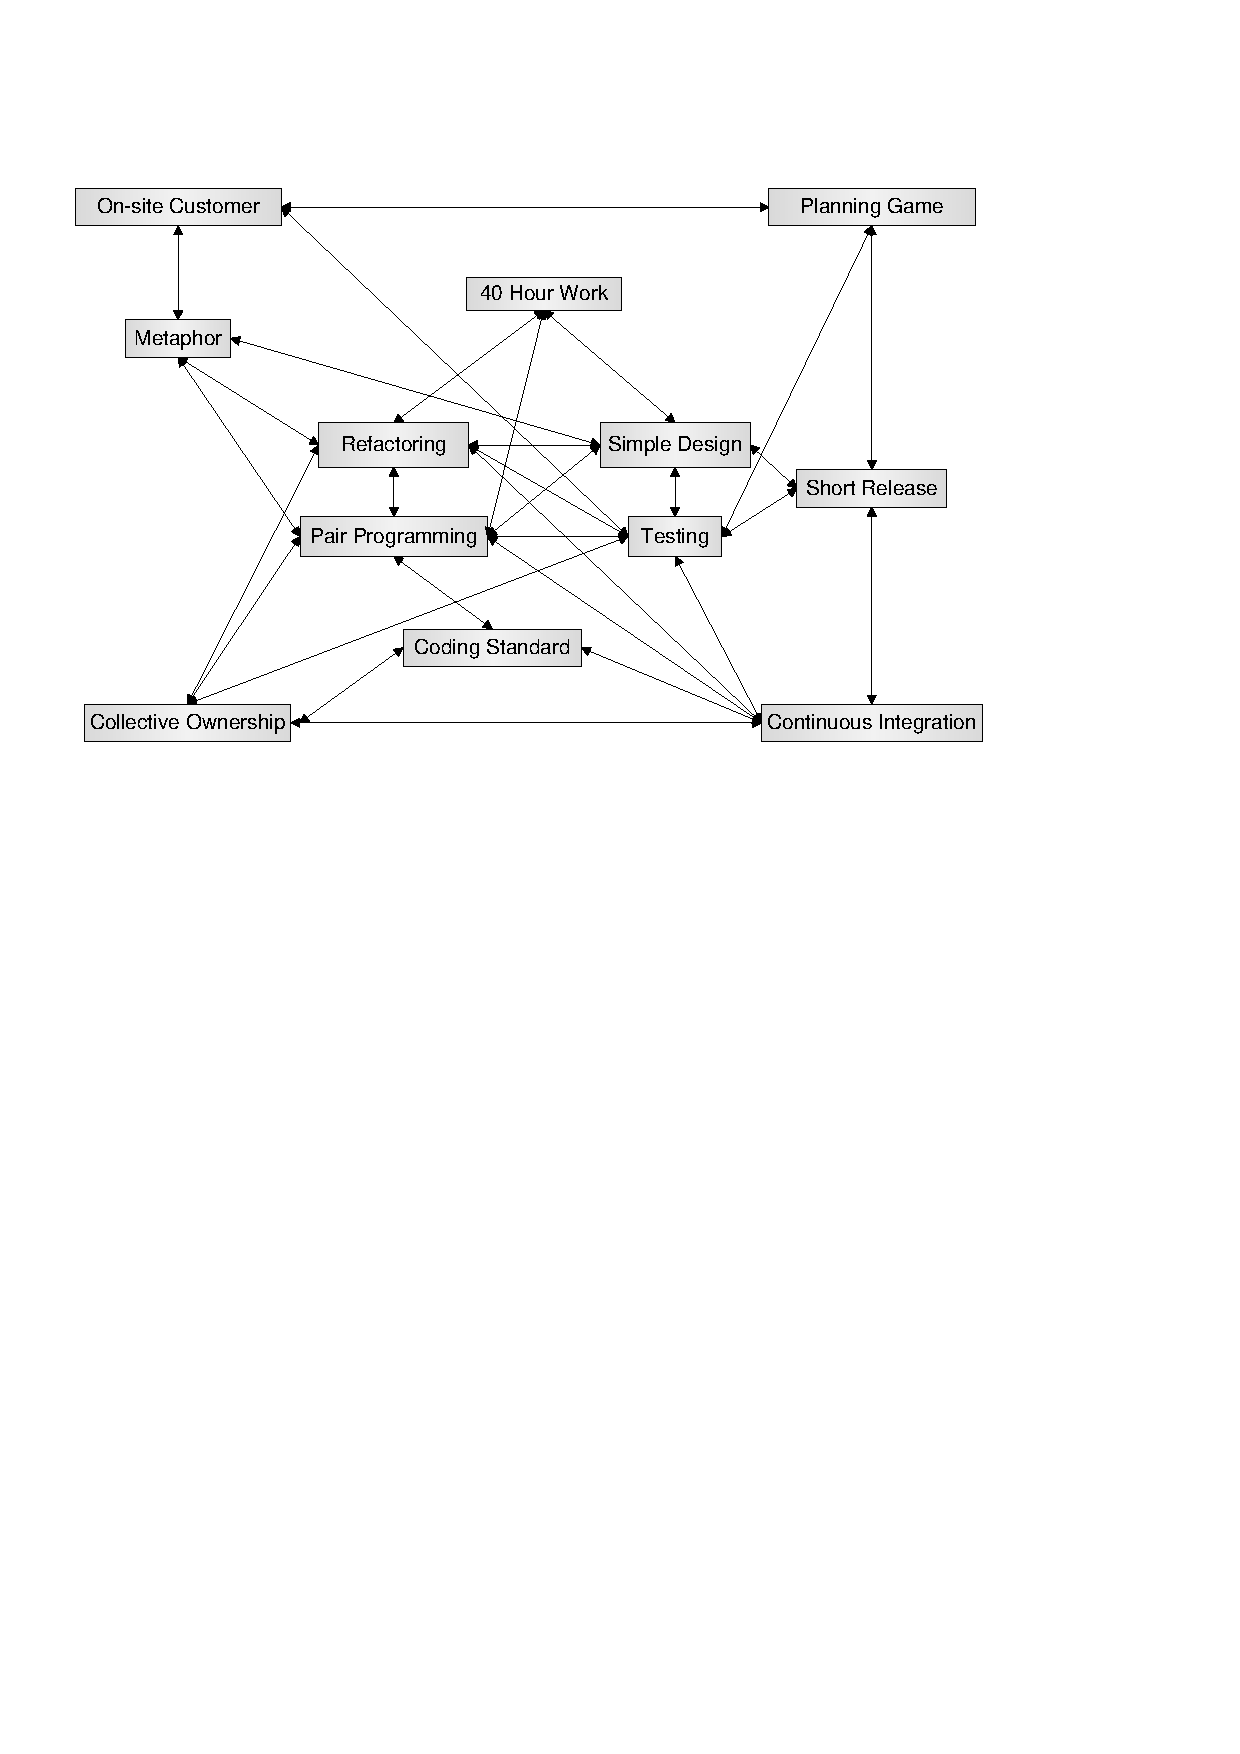
\includegraphics[width=0.6\textwidth]{figs/Visio-XPNetwork}
  \caption{Network of Extreme Programming Practices\cite{Beck:00}}
  \label{fig:XPNetwork}
\end{figure}
XP proposes TDD as the glue to hold the process together. TDD helps 
create a comprehensive suite of unit tests such that developers have 
the courage to consistently refactor code into a much simpler design.  

Though born as a practice of XP, TDD is often thought as an independent 
software development method. It can be used by practitioners and 
organizations that do not or partially practice XP 
\cite{Beck:03,TestDrivenWeb,TddYahooGroup}. Many TDD training workshops 
\cite{OsheroveWorkshop:04,ClarkwareWorkshop:04,
AdaptionTddWorkshop,IndustrialLogicTddWorkshop,TestDrivenDotComWeblogs,
BENUGWorkshop:04} have been provided by experienced practitioners 
and consulting companies. An informal 
survey \cite{UnitTestingPoll:06} conducted by the Method and 
Survey magazine found that 46\% of the studied software 
organizations perform unit testing informally, 41\% of the 
studied organizations document their unit test cases, and 
14\% of the studied organizations use the TDD approach.

\subsection{Characteristics of TDD}
\begin{quotation}
``\textit{Never write a line of functional code without a broken test case.}''

\raggedleft{--- Kent Beck}
\end{quotation}
\begin{quotation}
``\textit{Test first coding is not a testing technique.}'' 

\raggedleft{--- Ward Cunningham}
\end{quotation}

Recall that the two basic rules of TDD are to ``(1) Write new code 
only if an automated test has failed; (2) Eliminate duplication.''
Following the first rule, given a requirement, a TDD developer 
analyzes it first, and then outlines a To-Do list with a few tasks. 
The tasks can be very simple but should suffice to enable some 
development to occur. The developer can start a task that is either easy 
to do or essential to the problem to be solved 
\cite{Astels:03, Beck:03}. After picking a task, the developer 
writes a unit test first, and then invokes it. The test invocation 
might fail because it tests something that does not exist. The 
failing test drives the implementation of new functional code
to make it pass. Often, it is also necessary to run all tests to
make sure nothing is broken. The second rule is to eliminate
the duplication. If redundancy is introduced in the first
step, the developer should refactor either test code or functional
code to remove it. It is also necessary to run all tests 
after refactoring to confirm that nothing is broken. This 
is an iteration of TDD. A common belief is that TDD iterations 
should not last more than 10 minutes \cite{TDDRhythm}. 
After an iteration is over, the developer can cross out the
finished task from the To-Do list, and pick another task  
to begin a new iteration. Additionally, the developer should
add new tasks to the To-Do list whenever he or she wants. The 
characteristics of TDD are :
\subsubsection{Test First}
Test first is the key characteristic of TDD. Importantly, in 
TDD, developers should ``never write a line of functional 
code without a broken test case'' \cite{Beck:01}. 

\subsubsection{Short Iterations}
Quickly adding functional code to make test pass is important
to TDD. An iteration should last a few seconds to 
several minutes only. If hours of work is needed to make a 
test pass, probably the developer should divide the programming 
task into several sub tasks that can be solved in a shorter
period of time. 

\subsubsection{Frequent Refactoring}
Code is consistently refactored in TDD to create the simplest
possible design. The existence of a suite of unit tests gives 
developers the ``courage'' to refactor the code \cite{Beck:03}. 

\subsubsection{Rapid Feedback}
Unit testing is usually supported by the XUnit\cite{XUnit}
framework that is available in most mainstream languages. 
After new functional code is added, developers can invoke
the unit tests to test it right away. The feedback is available
within seconds or minutes. 

\subsubsection{One Ball in the Air at Once}
In typical software development, a developer usually carries 
a baggage with the requirement, system structure design, algorithm, 
code efficiency, readability and communication with other code 
etc. Martin Fowler described that the process is like keeping 
several balls in the air at once (Page 215 in \cite{Beck:03}), 
while the developer only keeps one ball in the air at once and 
concentrates on that ball properly in TDD. In the development
step, the developer only needs to make the test pass 
without worrying about whether it is a good or bad design. In 
the refactoring step, the developer only worries about what 
makes a good design. 

\subsubsection{Always Working Code}
The code should be always working in TDD because developers run 
all tests at the end of each iteration. If any test has failed, 
the developer should fix it right away. The fix should be easy because 
only a small amount of code is written in each iteration. If running 
all tests after an iteration is not feasible, the continuous 
integration can be set up to run them all once a day or several 
times a day. 

\subsection{Benefits of TDD to Software Development}

\begin{quotation}
``\textit{I have spent enough time in my career on silly 
bug-hunting, with TDD those days are gone. Yes, there are 
still bugs, but they are fewer and far less critical.}'' 
\cite{ExtremeJSBlog} 

\raggedleft{---Thomas Eyde}
\end{quotation}

The two most notable benefits of TDD are high quality
and developer productivity \cite{Beck:01,Janzen:05} :

\subsubsection{High Quality}
Probably the most advocated benefit of TDD is the high 
code quality. Because software quality is hard to measure, 
practitioners and researchers often use code coverage as 
the proxy of software quality. The code developed in TDD 
should be 100\% covered since no functional code is created 
without a unit test. 

\subsubsection{High Productivity}
Functional code and test code are both products. Testing is 
part of the design process, and it does not take a long time 
to write a small test. If developers need to write same amount 
of test code, TDD should save development time because less 
time is spent on tests than in the traditional test last or ad-hoc 
development methods. In addition, TDD users claim that the 
method reduces the overall amount of time spent on debugging, 
with a resulting increase in overall productivity\cite{Williams:03}.

% When and how TDD was developed
% Introduction to Extreme Programming
% XP and TDD are widely adopted in industry
% Benefit of TDD. Wide spread of TDD in the industry.
%
% Extensive research work has been conducted on Test-Driven Development

\section{TDD Research Work}
\label{sec:related-empirical}

Much research work has been conducted on studying important
outcomes of TDD such as software quality and developer productivity 
in recent years. In addition to anecdotal experience reports
\cite{George:04,Maximilien:03,Williams:03,Kaufmann:03,Edwards:04,Bhat:06}, 
researchers have run controlled experiments 
\cite{Muller:02,Matjaz:03,Erdogmus:05} to compare TDD against other 
development methods such as test last and ad hoc. Depending on whether
the test subjects are students or professional developers, the research
work can be categorized into academic and industrial studies.

\subsection{Empirical Evaluation in Academic Settings}

M\"{u}ller and Hanger \cite{Muller:02} conducted a study in an 
XP class in Germany to test TDD against traditional programming. 
The acceptance tests were provided 
to both the TDD group and the control group. Interestingly, students 
in the TDD group spent more time but their programs were less reliable 
than the control group.  

Edwards \cite{Edwards:04} adopted TDD in a junior-level class to compare
whether students got more reliable code after the use of TDD and WEB-CAT,
an assignment submission system. It turned out that the students using TDD
reduced their defect rate dramatically (45\% fewer defects/KSLOC using a
proxy metric) after adopting TDD, and a posttest survey found that TDD
students were more confident of the correctness and robustness of their
programs.

Similarly, Kaufmann and Janzen \cite{Kaufmann:03} conducted a pilot study 
on implications of TDD in an advanced project-oriented software 
engineering course. They also reported that TDD helped to improve software 
quality and programmers' confidence.

Pan\v{c}ur, Ciglari\v{c}, Trampu\v{s}, and Vidmar \cite{Matjaz:03} designed 
a controlled experiment to compare TDD with Iterative Test-Last approach 
(ITL), which is a slightly modified TDD development process in the order 
of ``code-test-refactor''.  This study
found that TDD is somewhat different from ITL but the difference is very
small. 

A more recent study on the effectiveness of TDD conducted by Erdogmus,
Morisio and Torchiano \cite{Erdogmus:05} used the well-defined test-last
and TDD approaches as Pan\v{c}ur did in \cite{Matjaz:03}. This study 
concluded that TDD programmers wrote more tests per unit of programming 
effort. More test code tends to increase software quality. Thus, TDD appears 
to improve the quality of software but TDD group in the study did not 
achieve better quality on average than test-last group. 

\subsection{Empirical Evaluation in Industrial Settings}
Several attempts have been made by researchers to study software quality
and developer productivity improvements of TDD in industrial settings.  

George and Williams \cite{George:04} ran a set of structured experiments
with 24 professional pair programmers in three companies. Each pair was
randomly assigned to a TDD group or a control group to develop a bowling
game application. The final projects were assessed at the end of the
experiment.  They found that TDD practice appears to yield code with
superior external code quality as measured by a set of blackbox test cases,
and TDD group passed 18\% more test cases. However, the TDD group spent
16\% more time on development, which could have indicated that achieving
higher quality requires some additional investment of time. Interestingly,
and in the contrast to the empirical findings, 78\% of the subjects
indicated that TDD practice would improve programmers' productivity.

Maximilien and Williams \cite{Maximilien:03} transitioned a software team
from an ad-hoc approach to testing to TDD unit testing practice at IBM, and
this team improved software quality by 50\% as measured by Functional
Verification Tests (FVT).

Williams, Maximilien, and Vouk \cite{Williams:03} conducted another case
study in IBM to study TDD. Compared to a baseline project developed in a 
traditional fashion, the defect density of the project developed 
in TDD was reduced by 40\% as measured by functional verification and 
regression tests. The productivity was not impacted by the additional 
focus on producing test code. 

Geras, Smith and Miller \cite{Geras:04} isolated TDD from other XP
practices, and investigated the impact of TDD on developer productivity and
software quality. In their research, TDD does not require more time but
developers in TDD group wrote more tests and executed them more frequently,
which may have led to future time savings on debugging and development.

Another study of TDD at Microsoft conducted by Bhat and Nagappan
\cite{Bhat:06} reported remarkable software quality improvement as 
measured in number of defects per KLOC. After introduction of TDD, 
project A (Windows) reduced its defects rate by 2.6 times, and project 
B (MSN) reduced its defect rate by 4.2 times, compared to the organizational
average. Reportedly, developers in project A spent 35\% more development
time, and developers in project B spent 15\% more development time, than
the developers in non-TDD projects spent.

\subsection{Discussion of Empirical Evaluation Studies}
The research findings of empirical studies are mixed on software quality 
and developer productivity as shown in Table \ref{tab:TDDResearchWork2}. 
The study conducted in Microsoft \cite{Bhat:06} and the study conducted 
in University of Karlsruhe \cite{Muller:02} are two extreme cases. In 
\cite{Bhat:06}, the developers improved software quality up to four 
times after adopting TDD. In comparison, the TDD group in \cite{Muller:02} 
yielded less reliable programs than the control group. In the following,
I will compare the research results according to the differences in
experiment settings. 

\begin{sidewaystable}[htbp]
\centering
  \begin{tabular}{|l|l|l|l|l|l|} \hline 
 & Investigator	& Study Type & Participants	& Software Quality	& Developer Productivity \\ \hline
 & George \cite{George:03} & Controlled Experiment	& 24	& TDD passed 18\% more tests & 16\% more time \\ \cline{2-6}
 & Geras \cite{Geras:04}  &  Controlled Experiment & 14	& TDD has the edge on quality & No impact \\ \cline{2-6}
 Industrial
 & Maximilien	\cite{Maximilien:03} & Case Study &  9	& 50\% reduction in defect density	& Minimal impact \\ \cline{2-6}
 & Williams\cite{Williams:03} & Case Study & 9	& 40\% reduction in defect density	& No change \\ \cline{2-6}
 & Bhat	\cite{Bhat:06}  & Case Study & 11	& 2-4 times reduction in defect density	& 35\% and 15\% more time \\ 
 
 \hline \hline
 
         & Kaufmann \cite{Kaufmann:03}	& Controlled Experiment &  8	& N/A	    & 50\% improvement \\ \cline{2-6}
         & Edwards \cite{Edwards:04} & Case Study & 59	& 54\% fewer defects	& N/A \\ \cline{2-6}
Academic & Erdogmus	\cite{Erdogmus:05} & Controlled Experiment & 35	& No change	  & Improved productivity \\ \cline{2-6}
         & M\"{u}ller \cite{Muller:02} & Controlled Experiment & 19 & Less reliable, but better reuse	& No change \\ \cline{2-6}
         & Pan\v{c}ur	\cite{Matjaz:03} & Controlled Experiment & 38	& No change	  & No change \\ \hline
  \end{tabular}
  \caption{Research Work of TDD on Software Quality and Developer Productivity}
  \label{tab:TDDResearchWork2}
\end{sidewaystable}


\subsubsection{Students vs. Professional Developers}
One difference is in population. The studies in academic settings 
used students as test subjects, while the studies in industrial 
settings recruited professional developers. 
Of 10 empirical studies listed in Table \ref{tab:TDDResearchWork2},
5 were conducted in academic settings, and the other 5 were 
conducted in industrial settings. The 
studies conducted in industrial settings found evidence of 
software quality improvements, but often at the cost of 
decrease of developer productivity. On the contrary, the 
studies in academic settings often found no software quality 
improvement but increase of developer productivity. 

How come the research findings are so divided among studies 
conducted within different population? Did professional 
developers pay more attention to software quality than 
students? Were students more concerned about productivity
than professional developers?  A caveat of industrial studies 
is that they must be beneficial to participants. 
In \cite{Maximilien:03}, Maximilien and Williams proposed TDD as 
a solution to reduce the defect rate. In \cite{Williams:03}, Williams,
Maximilien and Voulk assigned a dedicated coach to the development 
team. George and Williams \cite{George:03} noticed that the control 
group did not write worthwhile automated tests, partially due to the 
lack of incentives. Brilliant and Knight \cite{Brilliant:99} note 
that industry does not perceive a significant benefit from working 
with academic researchers in many cases. Researchers have to be able
to convince industry practitioners of the benefits and provide 
assistance in order to conduct research in industrial settings. 
The benefits are important to the participants of industrial studies, 
otherwise the quality of research would degrade. Geras, Smith and 
Miller reported that professional developers are hard to recruit 
when participation is voluntary \cite{Geras:04}. 

Students are generally less experienced at software development 
when compared to professional software developers. It is unclear 
whether students are appropriate participants for effectively
studying TDD \cite{Erdogmus:05}. M\"{u}ller and Hagner reported 
that the TDD group produced code with 74\% branch converage only, while the control 
group produced code with 80\% branch coverage \cite{Muller:02}. 
Erdogmus, Morisio and Torchiano \cite{Erdogmus:05} discussed 
the causal relationship between research findings and participant 
skill levels. They found that the students with high skill rate 
improved productivity more dramatically than the students with 
low skill rate. 

\subsubsection{Case Study vs. Controlled Experiment}
Another difference between the academic and industry based research
is in research methods. Case study and 
controlled experiment are the two most popular research methods. 
Of the 10 studies listed in Table \ref{tab:TDDResearchWork2}, 6 
are controlled experiments and 4 are case studies. Most of the
controlled experiments were conducted in academic settings because
classroom settings are more amenable to controlled experimentation. 
Since industry rarely repeats the same project twice, it is hard to have 
controlled experiments in industrial settings. Three out 
of five industrial studies were case studies. 

In controlled experiments, researchers often isolated test
first from TDD to compare it against other development 
methods such as test last and ad-hoc \cite{Muller:02,Matjaz:03,
Erdogmus:05,George:03,Geras:04}. Half of the controlled 
experiments \cite{George:03,Kaufmann:03,Erdogmus:05} observed 
productivity improvement in TDD groups, but only two studies 
found evidence of software quality improvement. On the contrary, 
the participants in the case studies improved software quality 
dramatically after adopting TDD, but they also spent more time 
on development.  

\subsubsection{Rivalry Development Methods}
The third difference of experiment settings is in the 
development methods that TDD was compared against. Researchers 
compared TDD against the traditional test-last\cite{Kaufmann:03,Geras:04}, 
ad hoc\cite{Muller:02,George:03}, and iterative test last 
(ITL) \cite{Matjaz:03,Erdogmus:05} methods. TDD did not help to 
improve software quality when it was compared against ITL. 
But it helped to improve software quality when it was compared 
with ad hoc and test last methods. Though TDD developers 
spent more development time, they also wrote more tests 
\cite{George:03,Erdogmus:05} and ran tests more frequently
\cite{Geras:04}.

\subsection{Process Conformance of TDD}
In the previous section, I have discussed the mixed research 
findings of TDD due to differences in population, research 
methods and the development methods that TDD was compared 
to. However, the research findings of studies in the same group  
were often consistent. For example, all the case studies found 
evidence of software quality improvement of TDD. Perhaps this 
phenomenon indicates that there are flaws in the empirical
studies of TDD. 

Erdogmus, Morisio and Torchiano \cite{Erdogmus:05} discussed that
a threat to the validity is ``process conformance'',
which is the level of conformance of the subjects
to the prescribed techniques. In order to improve process conformance,
they informed participants of the importance of following the 
proper procedures, and conducted a post test survey to filter 
unconformant data points\cite{Erdogmus:05}. Although they first
identified process conformance as a threat to the validity 
of research results of TDD, they were not alone in 
dealing with it. M\"uller and Hagner \cite{Muller:02} also 
indicated that their experiment was not technically controlled. 
During the experiment, they had to ask TDD groups if they were
following the test-first process. Pan\v{c}ur, Ciglari\v{c}, 
Trampu\v{s}, and Vidmar \cite{Matjaz:03} instrumented Eclipse, 
the development tool used in their study, to report unit test 
invocation frequency, results and time taken. A similar 
instrumentation method was used by Geras, Smith and Miller 
\cite{Geras:04}. However, instrumenting test invocation is 
a poor measure for process conformance of TDD because developers 
in test last groups can also run tests frequently. In 
\cite{George:03,Williams:03,Maximilien:03}, researchers studied 
test-first along with pair programming, which served as the 
process control method. Clearly, none of these methods is 
reliable at controlling participants' compliance to TDD or 
the rivalry development methods. 

Test first is a key characteristic of TDD, and developers 
should ``never write a line of functional code without a broken 
test case.'' \cite{Beck:01}. Short iterations, frequent 
refactoring, one ball in the air at once, and always working 
code are other characteristics of TDD. Developing software in 
TDD needs skills, practice, and discipline. On one hand, it is 
being widely adopted and embraced by software industry. Many 
developers simply enjoy the ``dance'' of test first and claim that
they are ``test-infected'', a phrase that is often used by the 
members of TDD community. On the other hand, the empirical research 
findings of TDD are often mixed. One of the causes of 
confused research results is the process conformance problem. 
In my thesis research, I have focussed on developing an automated 
machinery to evaluate the TDD conformance. Moreover, this work 
can be extended to study other low-level software processes as 
well. In a broader view, my work belongs to the research of automated 
software process. Some work has been conducted on this 
direction \cite{Cook:95,Cook:96,Jensen:04,Jensen:05}.

% We must collect low-level development behaviors in order
% to understand why TDD is employed and how it is used. 

\section{Automated Software Process Research}
\label{sec:related-automation}
Software process research is historically top-down. Process
programming\cite{Sutton:95}, modeling\cite{Curtis:92} and 
simulation\cite{Turnu:04,Jensen:05} are typical research 
methods for studying software processes. These top-down
methods are not usable for studying the process conformance of 
low-level software processes. They are appropriate when 
processes are confined and variations are very rare. 
However, these conditions are not easily met for low-level
software processes that define how developers should carry
on development activities at the granularity of minutes
and hours. Given a low-level software process, the actual 
process can be very different from the ideal process 
\cite{csdl-98-04,csdl2-06-01,csdl2-01-12}, which in turn leads 
to the issue of process conformance. 

In my research, I used a bottom-up research method. I applied 
rules on automatically gathered low-level development activities 
to infer the actual process, and compared the inferred process 
against the idealized process automatically, enabled by the 
rule-based system. My work is related to Cook's ``Automating 
Process Discovery and Validation'' and Jensen's ``Discovering 
and Modeling Open Source Software Processes'' because we all 
studied the automated evaluation of software processes using 
low-level development activities and software artifacts. 

%
% My thesis research focus is on designing an automated, 
% coherent framework to study the process conformance 
% of low-level software processes. 

\subsection{Automating Process Discovery and Validation}
Cook and Wolf \cite{Cook:95,Cook:96} developed a client-server 
system named Balboa to automate the process discovery using 
finite state machine (FSM). Balboa collects developers' 
invocations of Unix commands and CVS commits to construct
event streams. It then uses a neural network, a MARKOV chain, 
and data mining algorithms to discover 
the FSM of software processes. With Balboa, Cook and Wolf 
were able to reproduce the ISPW 6/7 process in their research. 
Figure \ref{fig:Balboa} illustrates the ISPW 6/7 process they 
discovered using the Markov Model.
\begin{figure}[htbp]
  \centering
  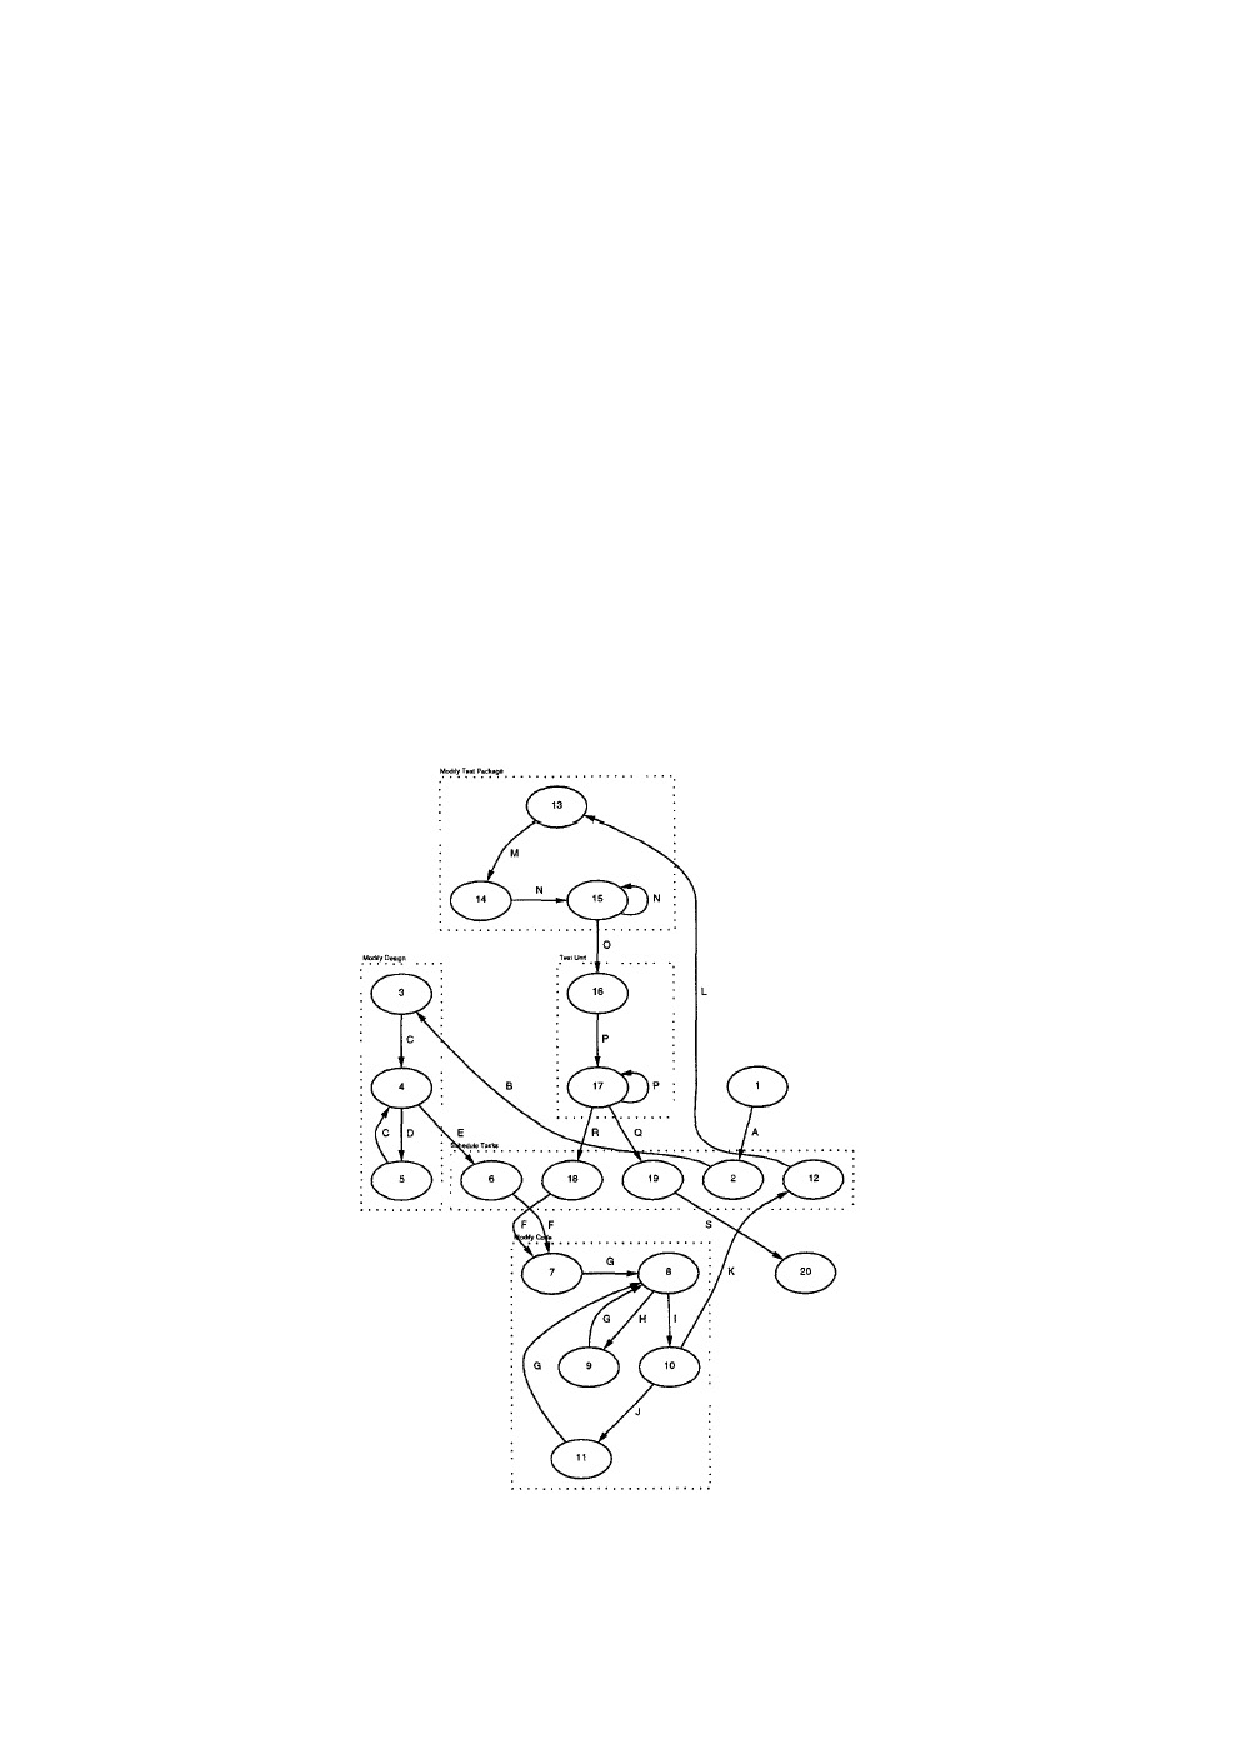
\includegraphics[width=0.6\textwidth]{figs/Balboa}
  \caption{Discovery of ISPW 6/7 Process (MARKOV )\cite{Cook:95}}
  \label{fig:Balboa}
\end{figure}
The numbered circles in Figure \ref{fig:Balboa} are the process 
states, and the arrows represent the development event data. 
Although Cook demonstrated that the generated FSM in Figure 
\ref{fig:Balboa} is very close to the actual ISPW 6/7 process, 
FSM does not look like an ideal technique for automated process
discovery and validation. The process FSM can be too complicated
to be useful. In \cite{Cook:95}, the three algorithms RNET, KTAIL
and MARKOV generated 15, 20 and 25 states respectively, and the 
states are interwoven in complicated manners as shown in Figure 
\ref{fig:Balboa}. It is very hard to interpret the monolithic 
state chart without a thorough understanding of Balboa and the 
adopted software process.

\begin{comment}
The FSM illustrated in Figure \ref{fig:Balboa} was generated 
from a event stream with only 32 events :
\mbox{ABCDCEFGHGIJGIKLMNOPRFGIKLMNOPQS}.
To discover the process hidden in this event steam, RNET 
took 10.4 hours, KTAIL took 29.4 seconds, and the MARKOV 
model used 0.6 seconds on a Sparc 2 Sun workstation. 
\end{comment}

\subsection{Discovering and Modeling Open Source Software Processes}
Jansen and Scacchi \cite{Jensen:04,Jensen:05} simulated an 
automated approach to discover and model the open source 
software development processes. They took advantage of prior 
knowledge to discover the software development processes by 
modeling the process fragments using a PML description. Their 
prototype simulation found that they could detect unusually 
long activities and problematic cycles of activities. They 
suggested that a bottom-up strategy, together with a top-down 
process meta-modeling is suitable for automated process 
discovery. But they don't have a working software system except 
for a prototype implementation of the ``requirement and 
release'' process of the open source project NetBeans.

\subsection{Discussion of Automated Process Conformance Research}
Automated process conformance is essentially about 
knowledge discovery and data mining, in which ordered 
data streams are processed to discover and classify 
naturally recurring patterns. 

Cook and Wolf used artificial neural network with RNET algorithm, 
MARKOV probability model with Bayesian 
learning algorithm, and KTAIL algorithm to mine the development 
event streams for discovering software processes \cite{Cook:95}. 
But generating a monolithic process model represented in FSM 
does not appear to be a very usable solution for process conformance 
validation of complicated software processes. In addition, 
generating FSM is very time consuming according to the 
performance report \cite{Cook:95}.

Jansen and Scacchi \cite{Jensen:04} modeled the requirement and 
release process of a large open source project using PML. They 
applied the modeled process to examine the development activities 
and behaviors. This bottom-up strategy, together with a top-down 
process meta-modeling, seems more plausible than FSM for dealing
with complicated development behaviors.  

In my thesis research, after researching the knowledge discovery
and data mining algorithms and techniques, I chose a rule-based
system to study process conformance of low-level software 
processes. Instead of asking process experts to inspect the
FSM of the executed process as Cook and Wolf did \cite{Cook:95}, 
I converted the process knowledge into a set of rules and used them 
to infer the software development behaviors. My method
is very close to Jansen's and Scacchi's approach \cite{Jensen:04} 
except that I used rules rather than PML for process descriptions. 

An intriguing phenomenon of automated software process research
is the scarcity of directly related literature work. Perhaps this 
is due to the difficulty of collecting the process execution data. 
Cook and Wolf ignored the problem of data collection in their 
research and claimed that it is site-specific \cite{Cook:95}. 
Jansen and Scacchi took advantage of rich information on the web 
and hypothesized that the proposed model can be used for the 
process deployment, validation and improvement \cite{Jensen:04}. 

Fortunately, with the development of sophisticated software 
metrics collection system such as Hackystat, software 
development data can be collected automatically and unobtrusively \cite{Hackystat,csdl2-01-12,csdl2-01-13,csdl2-02-07}. In my thesis 
research, based upon low-level development activities collected by 
Hackystat sensors, I conducted the research of the process conformance 
of Test-Driven Development. 

Wang and Erdogmus \cite{Wang:04} argued that the empirical research 
of TDD suffers from the construct validity problem (as is also the 
case in some other empirical software engineering research) because 
it lacks process conformance. They developed a prototype called 
``TestFirstGauge'' to study the process conformance 
of TDD by mining the in-process log data collected by Hackystat. 
TestFirstGauge aggregates software development data collected
by Hackystat to derive programming cycles of TDD. They used T/P ratio 
(lines of test code verse lines of production code), testing effort 
against production effort and cycle time distribution as the indicator 
of TDD process conformance. This project precedes the Zorro software 
system\cite{csdl2-06-02}, and in fact it stimulated our research interest 
in studying low-level software process conformance. Unlike the
prototype implementation of TestFirstGauge in VBA using an Excel
spreadsheet, Zorro is integrated into the Hackystat system for automation,
reuse, and flexibility using rule-based system \cite{Friedman-Hill:03}.

Similarly, Wege \cite{Wege:04} also focused on automated support of TDD
process assessment, but his work has a limitation in that it uses the CVS
history of code. Developers will not commit on-going project data at the
granularity of seconds, minutes or hours when they develop the software
system, making this data collection technique problematic for the purpose
of TDD inference. Collecting rapid low-level development activities is
a must in order to infer the low-level software process such as TDD
automatically.

%\subsection{Scientific Derivation and Simulation}

\section{Chapter Summary}

In this chapter, I introduced Test-Driven Development (TDD), a widely 
adopted core practice of Extreme Programming. The key characteristic
of TDD is to develop software by writing tests first. The software industry has 
widely adopted TDD and significant efforts have been put into it by 
practitioners (see Section \ref{sec:related-tdd}). Often, it is claimed 
that TDD can greatly help to improve software quality and developer 
productivity. The other claimed benefits of TDD include simple design, 
programmer confidence, and time 
saving on maintenance because less time is needed for bug hunting and 
debugging (see Section \ref{sec:related-tdd}). Much research work has been 
conducted on TDD about software quality and developer productivity 
(see Section \ref{sec:related-empirical}), but the research findings are 
divided. Interestingly, the research results are consistent
when the experiment settings were similar. A possible explanation 
for this phenomenon is process conformance, which is a construct validity
threat for the research findings (see Section \ref{sec:related-automation}). 

To address these problems and produce greater consistency in research 
results, I propose the automated process conformance inference with 
support from a rule-based system. In this chapter, I compared my research 
to Cook's automated process discovery and validation, Jansen's simulation 
of open source software project process, Wang's and Erdogmus's TestFirstGauge 
project, and Wege's automated support for process assessment in TDD 
(see Section \ref{sec:related-automation}).

\begin{comment}
Much of the research work on TDD suffers from the threat of ``construct
validity'' \cite{Wang:04} because of the what has been termed as the
``process conformance'' problem. Wang and Erdogmus defined process
conformance as the ability and willingness of the subjects to follow a
prescribed process.  Janzen warned that inability to accurately
characterize process conformance is harmful to TDD research
\cite{Janzen:05}: Many organizations might be using the methodology without
talking about it.  Others might claim to be using a methodology when in
fact they are misapplying it. Worse yet, they might be advertising its use
falsely.  Surveys might be conducted to gauge a method's usage, but often
only those who are much in favor or much opposed to the methodology will
respond.

A handful of research work has been done on software process validation
\cite{Cook:95,Jensen:05} and the process compliance of Test-Driven
Development \cite{csdl2-06-02,Wang:04,Wege:04}.  Cook and Wolf
\cite{Cook:95} developed a client-server software system called Balboa to
do process discovery and validation using a finite state machine (FSM).
Balboa collects developers' invocations of Unix commands and CVS commits to
learn the software process using FSM and machine learning techniques. Cook was 
able to reproduce the ISPW
6/7 process with Balboa in his research.  However, FSM does not look like
an ideal solution for process validation because of the complexity of the
process FSM it generates. In his example, the three algorithms RNET, KTAIL
and MARKOV generated 15, 20 and 25 states respectively, and the states are
interwoven in complicated manners. It is hard to interpret the process
state chart without thorough understanding of Balboa and the adopted
software process. Jansen and Scacchi \cite{Jensen:05} simulated an
automated approach to discovery and modeling of open source software
development processes.  They took advantage of prior knowledge to discover
the software development processes by modeling the process fragments using
a PML description. Their prototype simulation found that they could detect
unusually long activities and problematic cycles of activities. They
suggested that a bottom-up strategy, together with a top-down process
meta-modeling is suitable for automated process discovery. But they don't
have a working software system except for a prototype implementation.

Janzen \cite{Janzen:05} claimed that TDD is a kind of software development
method, not a process model, and that it has emerged out of a particular
set of process models. In contrast, Beck and Cunningham, the pioneers of
TDD, put it this way: ``test-first coding is not a testing technique but is
rather about design.''\cite{Beck:01} If TDD is a design technique and it
drives the implementation of product code, then classifying it as a
software process sounds reasonable. In my research, I have characterized
practices such as Test-Driven Development and Personal Software Process
(PSP) as low-level software processes. A common characteristic of a low-level
software process is that it is defined by many frequent and rapid
short-duration activities. Unlike high-level and long duration phases such
as ``requirement analysis'' that might last weeks to months, the activities
in low-level software process such as ``refactor class Foo to extract
interface IFoo'' may take only seconds to a few minutes \cite{csdl2-06-02}.

Low-level software processes often face similar research questions as
other, longer duration software processes. For instance, what process is
currently occurring, what process should occur, what are the impacts of a
given process on the important outcomes of software such as quality and
productivity, and how can a given process be improved and tailored in an
organization? So far, software engineering researchers have focused heavily
on the important outcomes that TDD brings to software products and software
developers. Both pedagogical
\cite{Muller:02,Edwards:04,Geras:04,Matjaz:03,Erdogmus:05,Kaufmann:03} and
industrial \cite{George:03,Maximilien:03,Bhat:06} evaluations of TDD have
been conducted in the last few years.  It is interesting to note that number of
research studies on TDD in academic settings is greater than the number of
research studies in industrial settings.

\section{Research Work in Academic Settings}
Most TDD research studies in academic settings seems to indicate that there
is some degree of quality improvement, but that there are little programmer
productivity benefits. Indeed, some studies have shown quality improvements
but at the cost of decreased productivity.

M\"{u}ller and Hanger \cite{Muller:02} conducted a study in an XP class in
Germany to test TDD in isolation of other XP practices against traditional
programming.  The acceptance tests were provided to both the TDD group and
the control group. Interestingly, students in the TDD group spent more time
but their programs were less reliable than the control group.  

Edwards \cite{Edwards:04} adopted TDD in a junior-level class to compare
whether students got more reliable code after the use of TDD and WEB-CAT,
an assignment submission system. It turned out that the students using TDD
reduced their defect rate dramatically (45\% fewer defects/KSLOC using a
proxy metric) after adopting TDD, and a posttest survey found that TDD
students were more confident of the correctness and robustness of their
programs.

Geras, Smith and Miller \cite{Geras:04} also isolated TDD from other XP
practices, and investigated the impact of TDD on developer productivity and
software quality. In their research, TDD does not require more time but
developers in TDD group wrote more tests and executed them more frequently,
which may have led to future time savings on debugging and development.

Pan\v{c}ur,Ciglari\v{c},Trampu\v{s}, and Vidmar \cite{Matjaz:03} designed 
a controlled experiment to compare TDD with Iterative Test-Last approach (ITL), 
which is a slightly modified TDD development process in the order of 
``code-test-refactor''.  This study found that TDD is somewhat different from 
ITL but the difference is very small.

A more recent study on the effectiveness of TDD conducted by Erdogmus,
Morisio and Torchiano \cite{Erdogmus:05} used the well-defined test-last
and TDD approaches as Pan\v{c}ur et al. did in \cite{Matjaz:03}. This study concluded
that TDD programmers wrote more tests per unit of programming effort. More
test code tends to increase software quality. Thus, TDD appears to improve
the quality of software but TDD group in the study did not achieve better
quality on average than test-last group.

Kaufmann \cite{Kaufmann:03}'s pilot study on implications of TDD, in
contrast, reported improved software quality and programmers' confidence.

\section{Research Work in Industrial Settings}
Several attempts have been made by researchers to study software quality
and productivity improvements of TDD in industrial settings.  

George and Williams \cite{George:04} ran a set of structured experiments
with 24 professional pair programmers in three companies. Each pair was
randomly assigned to a TDD group or a control group to develop a bowling
game application. The final projects were assessed at the end of the
experiment.  They found that TDD practice appears to yield code with
superior external code quality as measured by a set of blackbox test cases,
and TDD group passed 18\% more test cases. However, the TDD group spent
16\% more time on development, which could have indicated that achieving
higher quality requires some additional investment of time. Interestingly,
and in the contrast to the empirical findings, 78\% of the subjects
indicated that TDD practice would improve programmers' productivity.

Maximilien and Williams \cite{Maximilien:03} transitioned a software team
from an ad-hoc approach to testing to TDD unit testing practice at IBM, and
this team improved software quality by 50\% as measured by Functional
Verification Tests (FVT).

Another study of TDD at Microsoft conducted by Bhat and Nagappan
\cite{Bhat:06} reported remarkable software quality improvement as measured
in number of defects per KLOC. After introducing of TDD, project A
(Windows) reduced its defects rate by 2.6 times, and project B (MSN)
reduced its defect rate by 4.2 times, compared to the organizational
average. Reportedly, developers in project A spent 35\% more development
time, and developers in project B spent 15\% more development time, than
the developers in non-TDD projects spent.

\section{Process Conformance Study of TDD}
As we can see from the literature, there are discrepancies in the empirical
findings across both educational settings and industrial settings. Sometimes the
discrepancies are dramatic, for example \cite{Muller:02} found that the TDD
group yielded less reliable programs than the control group, while
\cite{Bhat:06} reported that the TDD group improved software quality by 
over four times.

Wang and Erdogmus \cite{Wang:04} pointed out there are several
possibilities that might explain why there are the discrepancies in TDD
research findings. For example, discrepancies could occur due to
differences in populations, differences in teaching methods and materials,
and differences in the techniques by which TDD is compared. They argued
that TDD empirical software research lacks process conformance, and
therefore it suffers from the construct validity problem (as is also the
case in some other empirical software engineering research). In
\cite{Wang:04}, they developed a prototype called TestFirstGauge to study
the process conformance of TDD by mining the in-process log data collected
by Hackystat. TestFirstGauge aggregates software development data collected
by Hackystat to derive programming cycles of TDD. They use T/P ratio (lines
of test code verse lines of production code), testing effort against
production effort and cycle time distribution as the indicator of TDD
process conformance. This project precedes the Zorro software system
\cite{csdl2-06-02}, and in fact it stimulated our research interest in
studying low-level software process conformance. Unlike the
prototype implementation of TestFirstGauge in VBA using an Excel
spreadsheet, Zorro is integrated into the Hackystat system for automation,
reuse, and flexibility using rule-based system \cite{Friedman-Hill:03}.

Similarly, Wege \cite{Wege:04} also focused on automated support of TDD
process assessment, but his work has a limitation in that it uses the CVS
history of code. Developers will not commit on-going project data at the
granularity of seconds, minutes or hours when they develop the software
system, making this data collection technique problematic for the purpose
of TDD inference.
\end{comment}
\chapter{Software Development Stream Analysis (SDSA)}
\label{ch:Framework}

SDSA is a Hackystat extension that provides a generic framework for 
organizing various kinds of software metrics received by Hackystat 
into a form appropriate as input to a rule-based, time-series analysis 
(Figure \ref{fig:ZorroInfrastructure}). SDSA supports (1) construction 
of software development streams, (2) partition of software development 
streams, and (3) inference of development behaviors. 

The SDSA framework supports completely automated analysis, once configured.
First, the data collection is automated because SDSA uses software process 
metrics collected by Hackystat sensors. The sensors collect in-process software 
metrics automatically and unobtrusively. Second, the construction and 
partitioning of the software development stream is automated. SDSA reduces 
software process metrics into development activities for construction of a 
software development stream, which is then partitioned into episodes. Once 
a development stream has been partitioned into a sequence of episodes, 
SDSA can analyze the development behaviors in these episodes and classify 
them according to whatever process is under analysis. Finally, the inference 
process is also automated because SDSA uses JESS\cite{Friedman-Hill:03}, 
a rule-based system in Java. Developers can specify part or all of the 
studied process as a set of rules. 

The SDSA framework is designed to be customized for a specific software 
process of interest. Developers can selectively choose the event streams
to merge in the software development stream construction phase (see Section
\ref{sec:SDSA-Construction}). For a software process, developers can 
use different tokenizers to partition the development streams (see Section 
\ref{sec:SDSA-Partition}). Also, different rules can be supplied for 
development behaviors inference (see Section \ref{sec:SDSA-Inference}). 

This chapter begins with an introduction to the Hackystat framework
on which the SDSA framework is built, followed by a description
of the SDSA framework itself. 

%The SDSA framework reduces a series of
%software metrics into an event stream, generate software development
%stream by merging event streams 
%%Low-level software processes emphesizes on software developers. They
%%carry out software projects following best practices and guideline 
%%provided by the low-level software processes. 

\section{Hackystat}
Hackystat is an open source framework for automated collection and analysis
of software engineering process and product metrics. Hackystat supports 
unobtrusive data collection via specialized ``sensors'' that are attached 
to development environment tools. These sensors send structured ``sensor 
data type'' instances via SOAP to a web server for analysis via server-side 
Hackystat ``applications''. Over two dozen sensors are currently available, 
including sensors for IDEs (Emacs, Eclipse, Vim, VisualStudio, Idea), 
configuration management (CVS, Subversion), bug tracking (Jira, Bugzilla), 
testing and coverage (JUnit, CppUnit, Emma, JBlanket), 
system builds and packaging (Ant), 
static analysis (Checkstyle, PMD, FindBugs, LOCC, SCLC), and so forth.

Hackystat is tool, environment, and process independent. It does not 
presume a specific operating system platform, a specific integrated 
development environment, or a specific software process. It is designed
to be extensible. It provides not only generic services such as 
software metrics collection, persistence and retrieval, and project 
definition management for conglomerating discrete software metrics 
from both an individual and other project members, but also an 
extension mechanism where new modules (sensors or applications) 
can be added. Applications of the Hackystat framework in addition 
to SDSA include in-process project management \cite{csdl2-04-11}, high 
performance computing \cite{csdl2-04-22}, and software engineering
education \cite{csdl2-03-12}.

\subsection{Software Metrics Collection, Persistence, and Retrieval}
When developers are programming in a development environment tool with
its sensor installed and enabled, the sensor will collect both
the process and product metrics unobtrusively. The sensors then send
them via SOAP to a web server that hosts Hackystat.
The architecture of Hackystat is client-server. The \textit{``clients''} 
can be development environment such as Emacs, Eclipse, 
and Microsoft Visual Studio. The \textit{``server''} is the 
framework itself and its extended applications. On the server-side
Hackystat handles metrics data persistence automatically. It stores 
them in XML formats and implements a self-managed caching mechanism 
to retrieve them when requested by the applications. 

\subsection{Extension Mechanism}
The Hackystat system provides an extension mechanism to support new 
functionalities including sensor data types (metrics), sensors, 
applications, documentation, and so forth. Each functionality needs 
to specify a configuration file in XML saying what it is about and 
what part of Hackystat it will extend. For instance, if you are developing a 
new sensor for the Java development environment tool NetBeans, you 
will specify a sensor definition file such as netbeans.sensor.def.xml. 
It will include the sensor name and
what metrics it collects. The further information on how to implement 
an extended functionality can be found at the Hackystat home 
page:\textit{http://www.hackystat.org}. 

\section{SDSA Framework}
SDSA is an application extending the Hackystat framework. It organizes
various kinds of process metrics data into a time-series software 
development stream and conducts rule-based analyses. SDSA is
data oriented. Figure \ref{fig:SDSA-Workflow} illustrates its data model
and work flow. 
\begin{figure}[htbp]
  \centering
  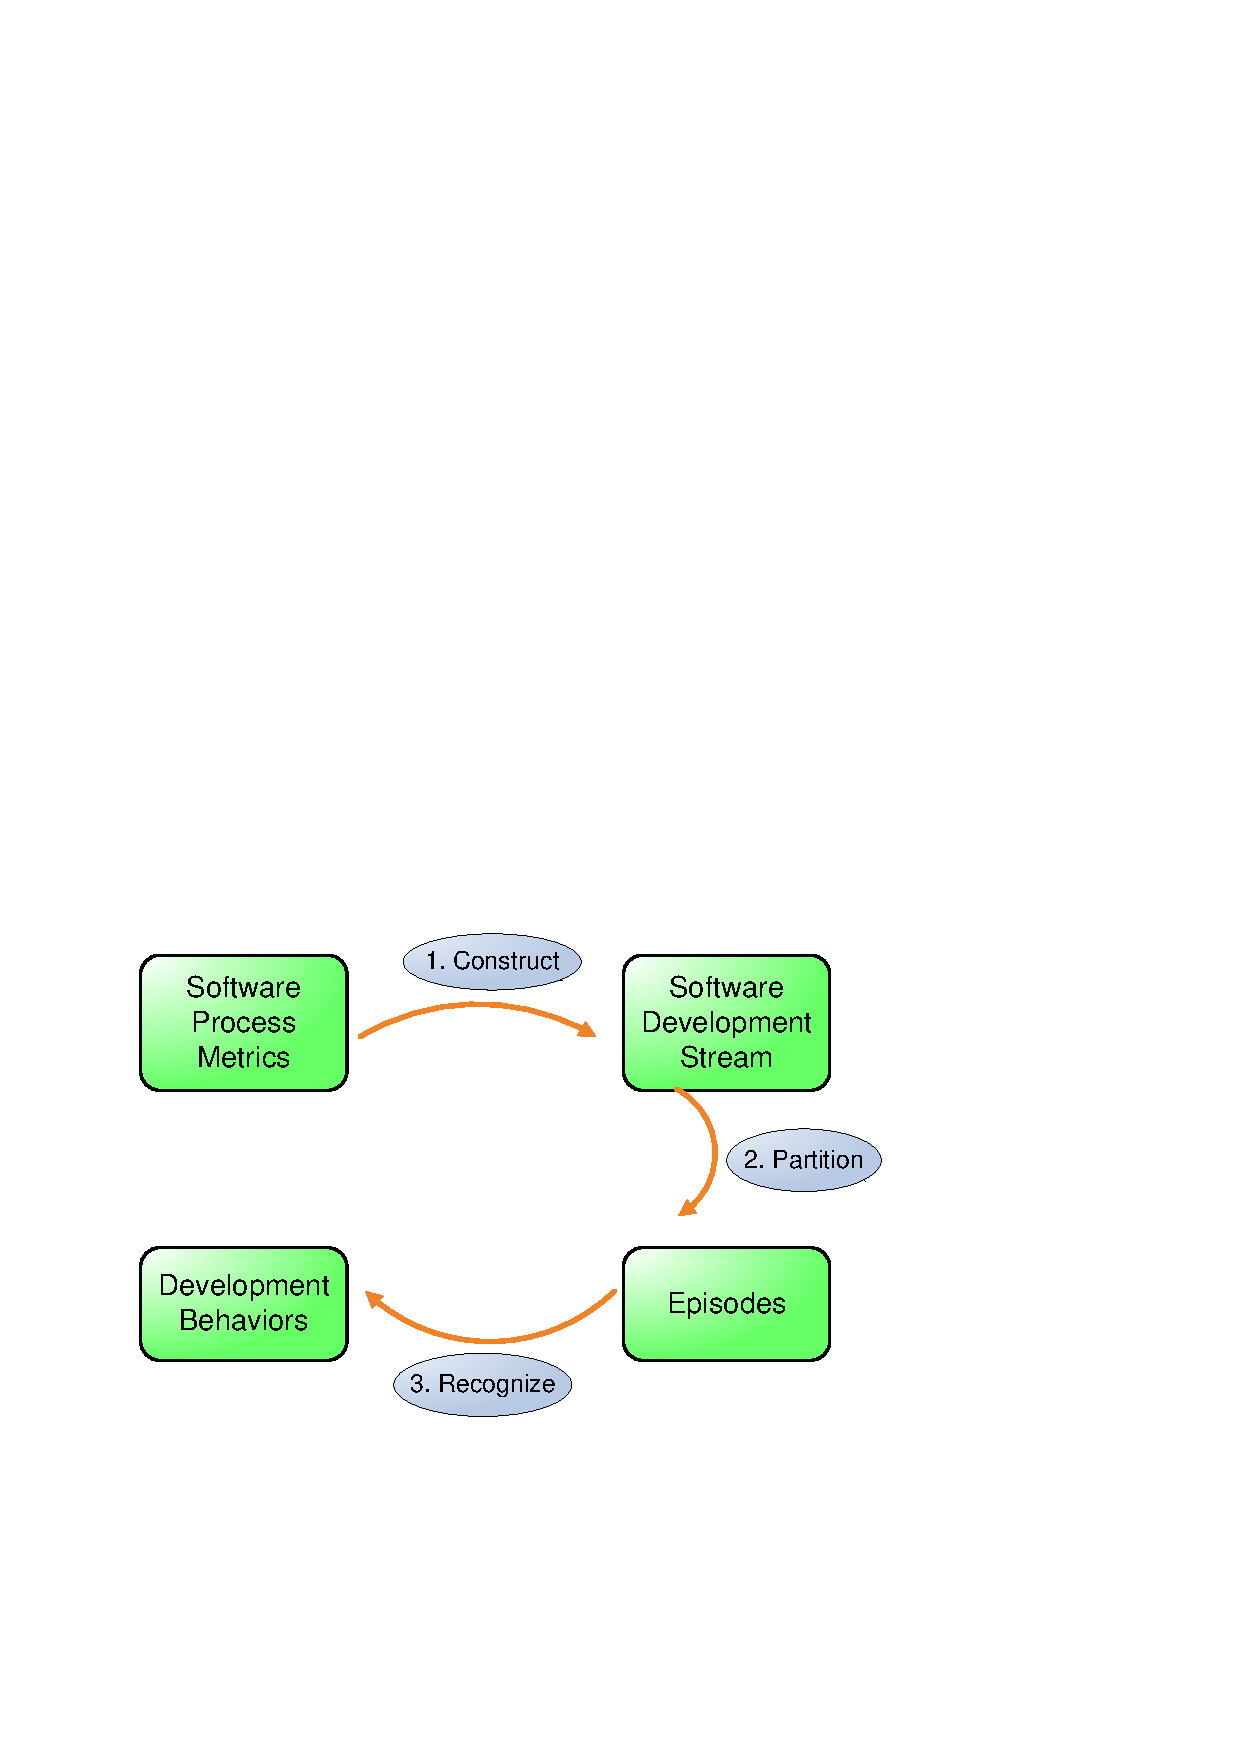
\includegraphics[width=0.5\textwidth]{figs/Visio-SDSA-FlowChart}
  \caption{Data Model and Work Flow of the SDSA Framework}
  \label{fig:SDSA-Workflow}
\end{figure}

SDSA models a software development process as a software development 
stream, which is a time-series data structure consisting of
continuous software development activities collected by Hackystat
sensors. The development stream 
is then partitioned into episodes delimited by boundary conditions. 
Each episode is a data model that represents an atomic components of 
the software process of interest. Eventually, the goal of SDSA is to 
recognize the development behaviors embodied within each episode. 

The data model breaks down the SDSA framework into three 
components(Figure \ref{fig:SDSA-Workflow}): (1) a software 
development stream construction subsystem, (2) a software 
development stream partition subsystem, and (3) a development 
behavior inference subsystem. 

\subsection{Software Development Stream Construction}
\label{sec:SDSA-Construction}
SDSA begins with the development stream construction subsystem 
that translates variety kinds of software process and product 
metrics into a development stream. Figure 
\ref{fig:SDSA-DevelopmentStream} illustrates the process
of software development stream construction. 
\begin{figure}[htbp]
  \centering
  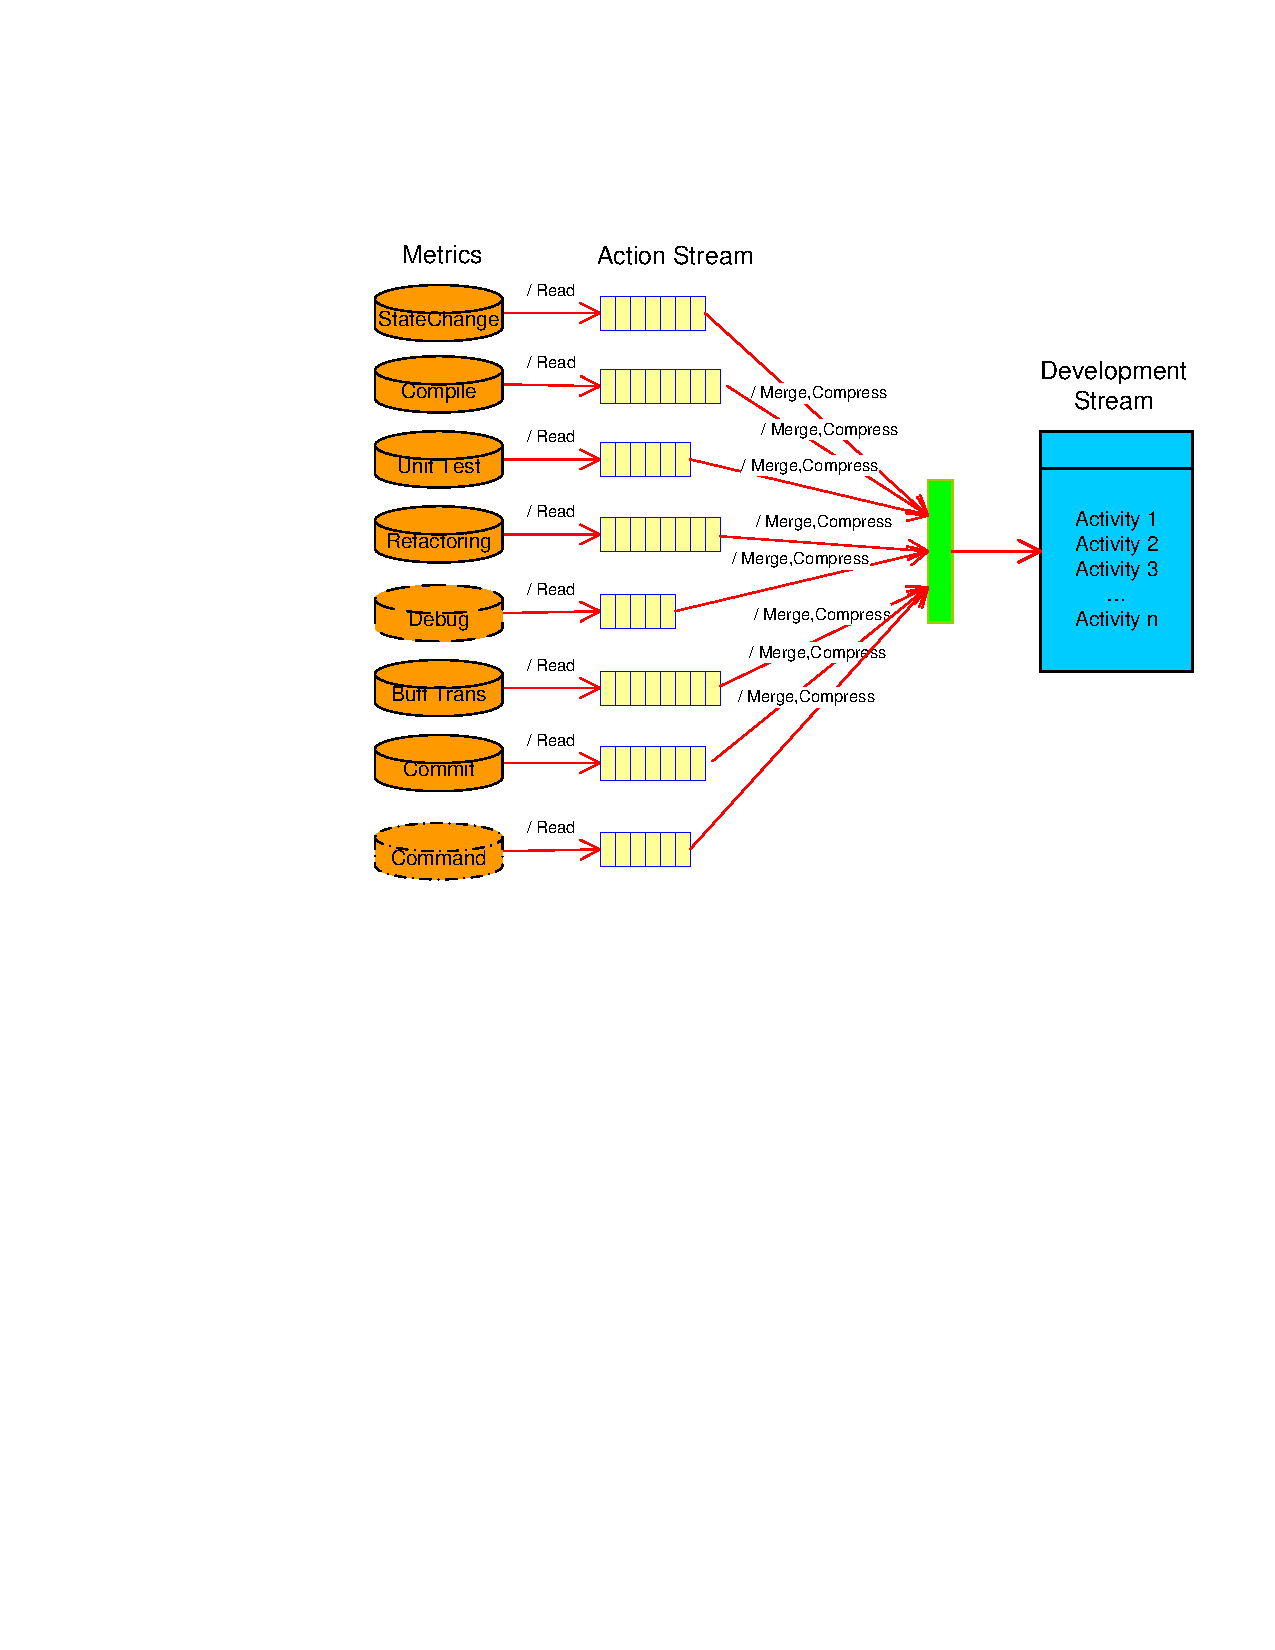
\includegraphics[width=0.8\textwidth]{figs/Visio-SDSA-DevelopmentStream}
  \caption{Software Development Stream Construction}
  \label{fig:SDSA-DevelopmentStream}
\end{figure}

Hackystat sensors collect the software process and product
metrics and abstract them as the structured ``sensor data type''. 
A sensor data entry represents a development activity or an
in-process product metric change that has been caused by a development 
activity. Because sensor data mixes software process and product 
metrics, SDSA must restructure them as development actions in order 
to infer the development behaviors. The development action is 
SDSA's internal representation of the software development 
activities that are collected by Hackystat sensors. 

\subsubsection{Development Action}
Figure \ref{fig:SDSA-Action-UML} is the class diagram of variety of 
development actions SDSA abstracted. All the development actions 
are subtypes of the ``Action'' type. Each action has a clock 
attribute indicating when it occurs and a duration attribute 
indicating how much time it takes. 

\begin{figure}[htbp]
  \centering
  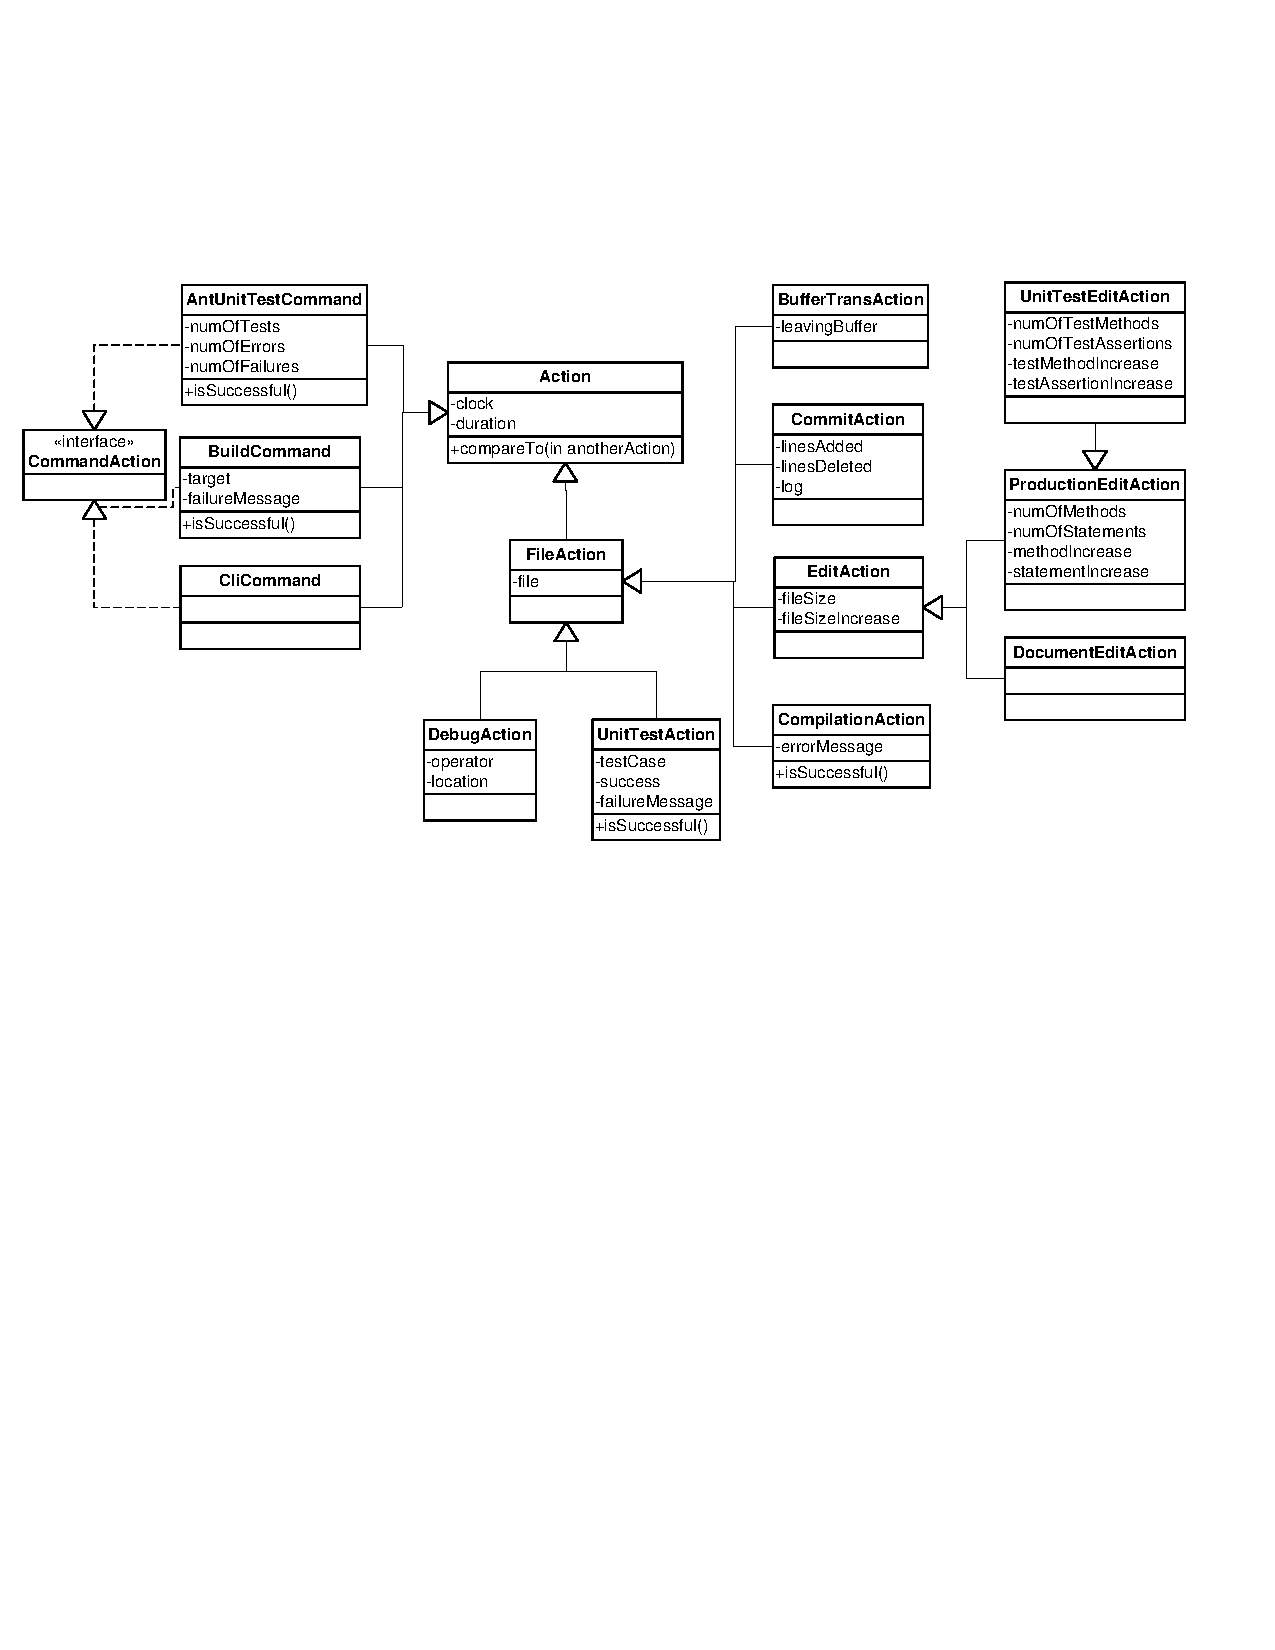
\includegraphics[width=0.9\textwidth]{figs/Visio-Action-UML}
  \caption{Class Diagram of Development Actions}
  \label{fig:SDSA-Action-UML}
\end{figure}

After reading the software metrics of a sensor data type, SDSA 
transforms them into development actions, and then forms 
a time-series action stream.

\subsubsection{Action Stream}
Figure \ref{fig:SDSA-ActionStream-UML} illustrates the class 
diagram of action streams. The ``DataStream'' is the super class 
of all action stream classes. Each action stream has the 
capability of transforming a type of sensor data into a 
time-series action stream. 

\begin{figure}[htbp]
  \centering
  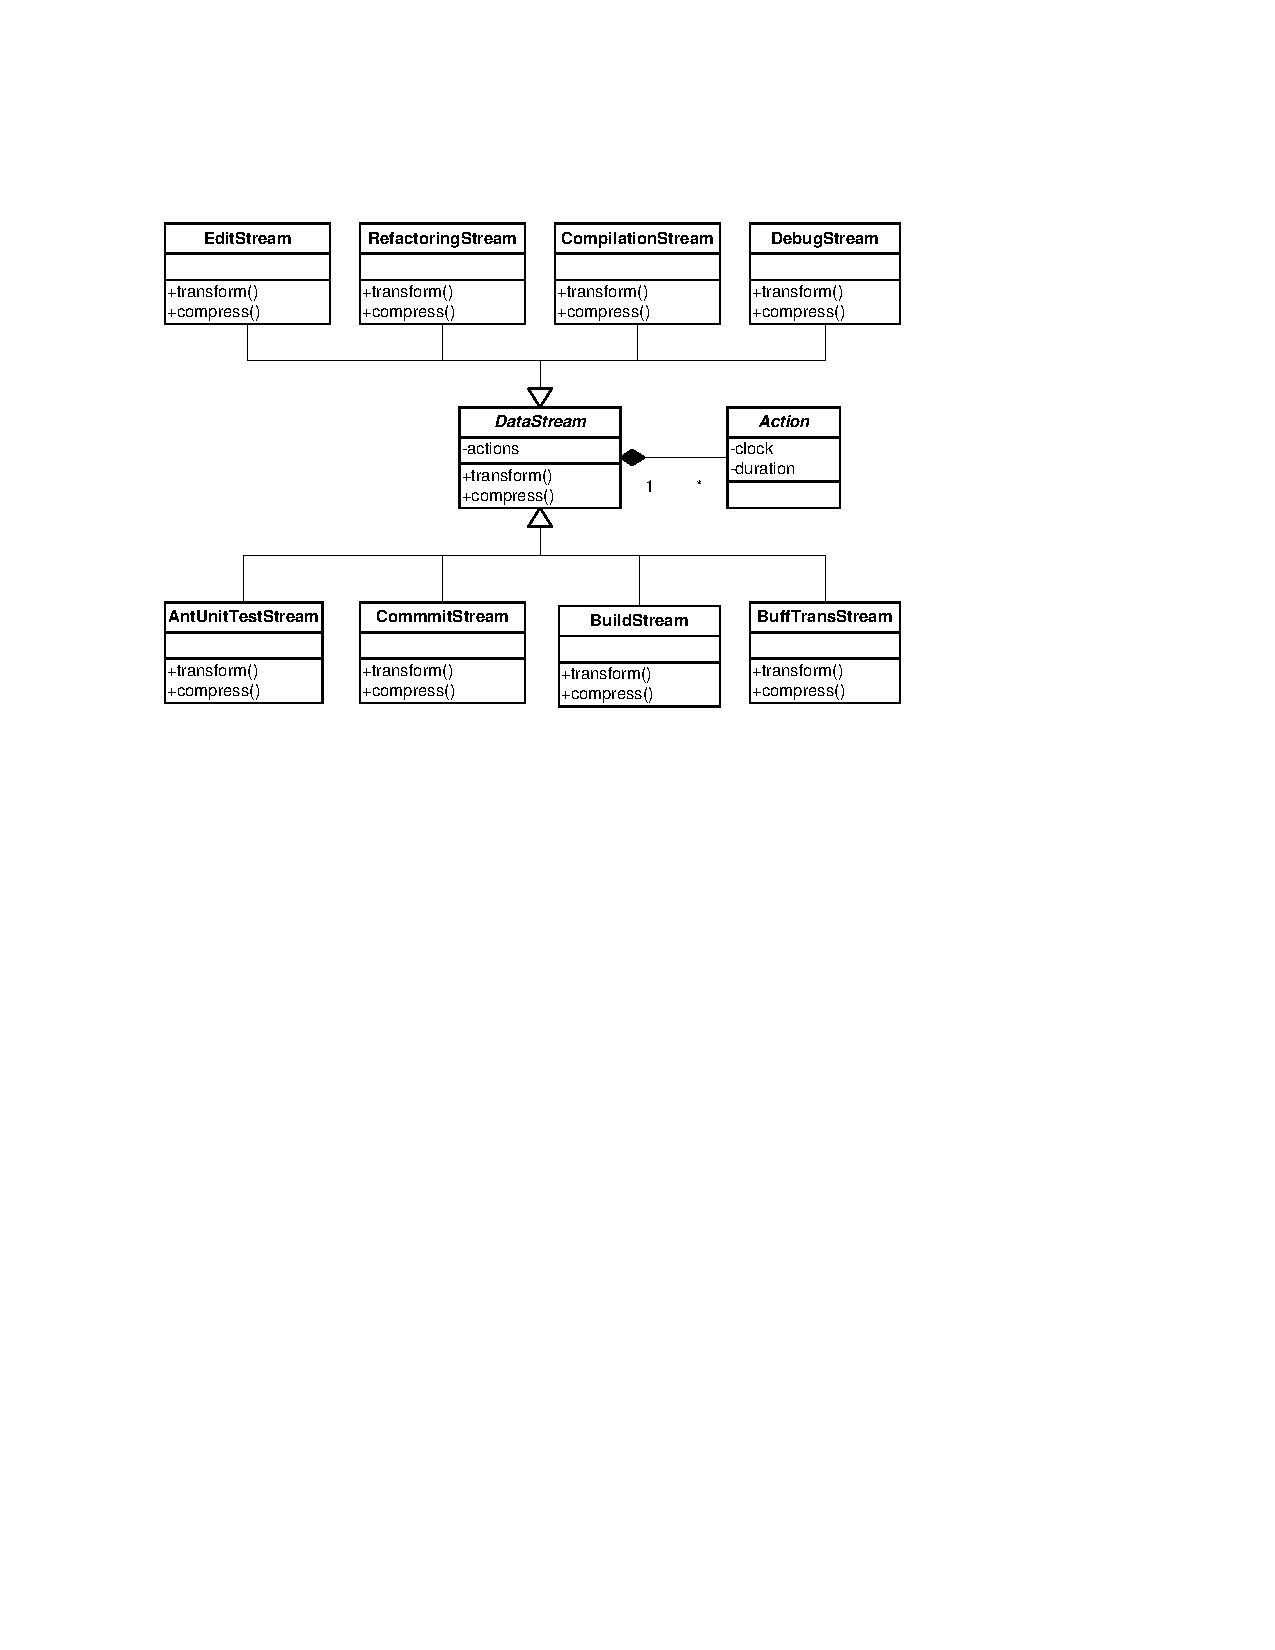
\includegraphics[width=0.8\textwidth]{figs/Visio-ActionStream-UML}
  \caption{Class Diagram of Action Streams}
  \label{fig:SDSA-ActionStream-UML}
\end{figure}

In addition to converting sensor data into development actions, 
an action stream can implement a callback function to compress 
itself. This function can group a set of continuous sensor data 
that represents a single development action. Using unit test 
invocation in the Eclipse IDE as an example, the Eclipse sensor 
collects and sends 3 ``UnitTest'' sensor data entries if the 
invoked unit test has 3 test cases. Because they are the 
consequence of a unit test invocation, the UnitTestStream 
can implement a compress function to group them into a single 
``UnitTest'' development action. 

\subsubsection{Development Stream}
Many kinds of action streams from a developer over a time 
period can merge together to form a software development stream 
as illustrated in Figure \ref{fig:SDSA-DevelopmentStream}. The 
``DevelopmentStream'' is an object representing a software
development stream. It is the container of action streams. The 
following code demonstrates the usage of ``DevelopmentStream''
class. Table \ref{tab:SDSA-StreamExample} is an example that shows
a software development stream's internal representations. 
\begin{verbatim}
   DevelopmentStream stream = 
       new DevelopmentStream(project, user, startDay, endDay);
   stream.addSubstream(new EditStream(user));
   stream.addSubstream(new BuffTransStream(user));
   stream.addSubstream(new RefactoringStream(user));
   stream.addSubstream(new UnitTestStream(user));
   stream.addSubstream(new CompilationStream(user));
   stream.assemble(); 
\end{verbatim}
\begin{table}[htbp]
  \caption{An Excerpt of a Software Development Stream}
  \begin{tabular}{|llll|} \hline
Time & File & Event & Metrics \\ \hline
12:35:29 & TestBowlingGame.java  & ADD METHOD  &	void TestGameCreation() \\ 
12:37:47 & TestBowlingGame.java  & TEST EDIT 	& 120sec MI=+1(3),SI=+1(4),TI=+1(3),AI=0(1) \\ 
12:38:07 & BowlingGame.java &	ADD CLASS &	BowlingGame.java \\ 
12:38:08 & BowlingGame.java &	BUFFTRANS &	FROM TestBowlingGame.java \\ 
12:38:13 & TestBowlingGame.java &	BUFFTRANS &	FROM BowlingGame.java \\ 
12:39:17 & TestBowlingGame.java &	TEST EDIT &	0sec MI=0(3),SI=-1(3),TI=0(3),AI=0(1) \\ 
12:39:17 & TestBowlingGame.java &	COMPILE &	The constructor Frame() is undefined \\
12:39:28 & BowlingGame.java &	ADD METHOD &	BowlingGame(Frame)\\
12:39:30 & BowlingGame.java &	BUFFTRANS &	FROM TestBowlingGame.java\\
12:39:35 & TestBowlingGame.java &	BUFFTRANS &	FROM BowlingGame.java\\
12:39:48 & BowlingGame.java &	PRODUCT EDIT &	0sec MI=+1(1),SI=0(0),FI=+124(124)\\
12:39:50 & BowlingGame.java &	BUFFTRANS &	FROM TestBowlingGame.java\\ \hline
  \end{tabular}
  \label{tab:SDSA-StreamExample}
\end{table}

\begin{comment}
Hackystat sensors can collect many kinds of software process metrics
including editing, compilation, unit testing, refactoring, and 
so forth. SDSA transforms these software metrics into development
events and builds event streams out of them. A development event
in SDSA has basic information such as time stamp, the target file,
duration etc. An event stream collects and sorts the development 
events from a kind in time sequence. Developers can select event
streams to merge for creating the software development stream (SDS). 

For example, the ``State Change'' sensor data type is 
an innovative approach collecting developer' editing activities in a
development environment indirectly. As a result, an editing activity
can be represented by one or several ``State Change'' sensor data
entries. 


The SDS is an abstraction of time-series software development events. 
One purpose of SDSA is to mine the sequential development streams to 
understand executions of low-level software processes. The data-driven 
methods are amenable for analyzing SDS because it has massive 
development events. Machine Learning (ML) \cite{} is a very popular
data-driven method. 

Data-Driven
To understand the software process
behind a software development stream, one can easily think of
machine learning \cite{}. It has already been widely used in 
the pattern recognition and data classification in data mining
and bioinformatic research \cite{}. Some research \cite{} already 
studied how it can be used for understanding time-series data. 
Cook demonstrated in his research that the machine learning 
algorithms can potentially discover and validate software 
processes. Furthermore, the machine learning technique can be 
more effective in understanding data if it is being supervised. 

Goal-Driven

Software process research is typical top-down. The goal-driven
GQM software engineering paradigm. Simulating how a process
model can be adapted in the real situation is a standard 
research method \cite{}. 

Both data-driven and goal-driven research methods have their 
pros and cons. Data-Driven suffer local minimization or 
over fitting problems. Goal-Driven is too ideal to be applied
in the real settings. The process experts have to be hired 
to enforce the process data collection and analysis. In my 
research, I proposed to take a trade-off between the goal-driven
and data-driven research paradigms. As a result of my research, 
I came up with a marriage of software development stream
and episode behavior inference. 
\end{comment}

\subsection{Software Development Stream Partition}
\label{sec:SDSA-Partition}
The second component of SDSA is the software development stream 
partition subsystem. 
The software development stream is a time-series data structure
that may have hundreds to thousands development activities. Though
applying machine learning algorithm is plausible \cite{Cook:95}, 
I proposed a mechanism to partition the development streams into 
episodes using the boundary conditions (Figure \ref{fig:SDSA-Partition}).
\begin{figure}[htbp]
  \centering
  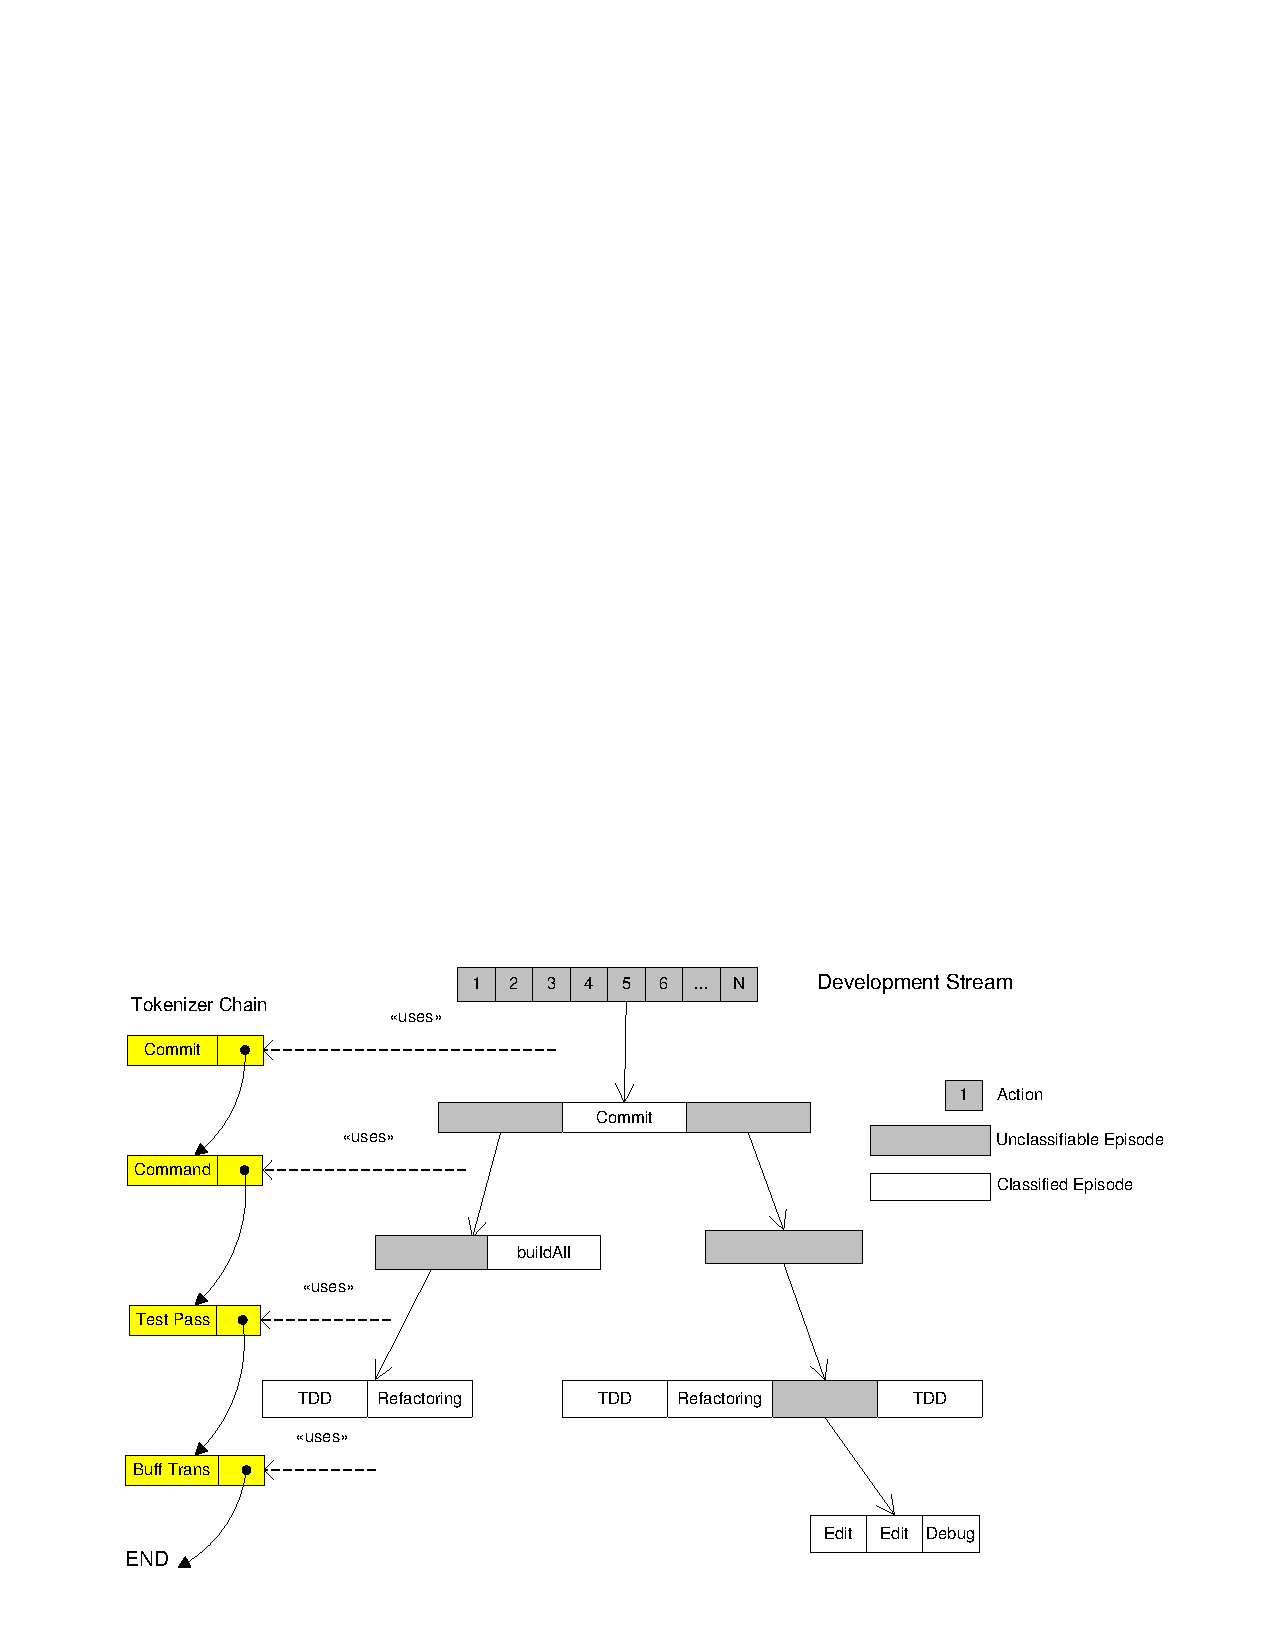
\includegraphics[width=0.8\textwidth]{figs/Visio-SDSA-Partition-UML}
  \caption{Partition of Development Stream}
  \label{fig:SDSA-Partition}
\end{figure}

Larman and Basili\cite{Larman:03} claim that the software development 
is iterative and incremental. Thus, tokenizing development streams not 
only simplifies mining large volumes of data, but also provides an approach 
to comparing actual software development processes to software process 
theories. Figure \ref{fig:SDSA-Partition} illustrates 
the design of the software development stream partition algorithm. 
Tokenizers, which partition software development streams using 
boundary conditions, can be chained together. Currently, four tokenizers 
have been developed in SDSA. Figure \ref{fig:SDSA-Tokenizers} illustrates 
their class diagram. Of course, developers can implement and add 
new tokenizers if necessary. 
\begin{itemize}
\item {\textbf{Commit Tokenizer}} partitions development streams by
source code repository commit actions.  

\item {\textbf{Command Tokenizer}} partitions development streams by
commands invoked in a shell window. 

\item {\textbf{Test Pass Tokenizer}} partitions development streams
by successful unit test invocations. 

\item {\textbf{Buffer Transition Tokenizer}} partitions development
streams by buffer changes in an IDE. 
\end{itemize}
\begin{figure}[htbp]
  \centering
  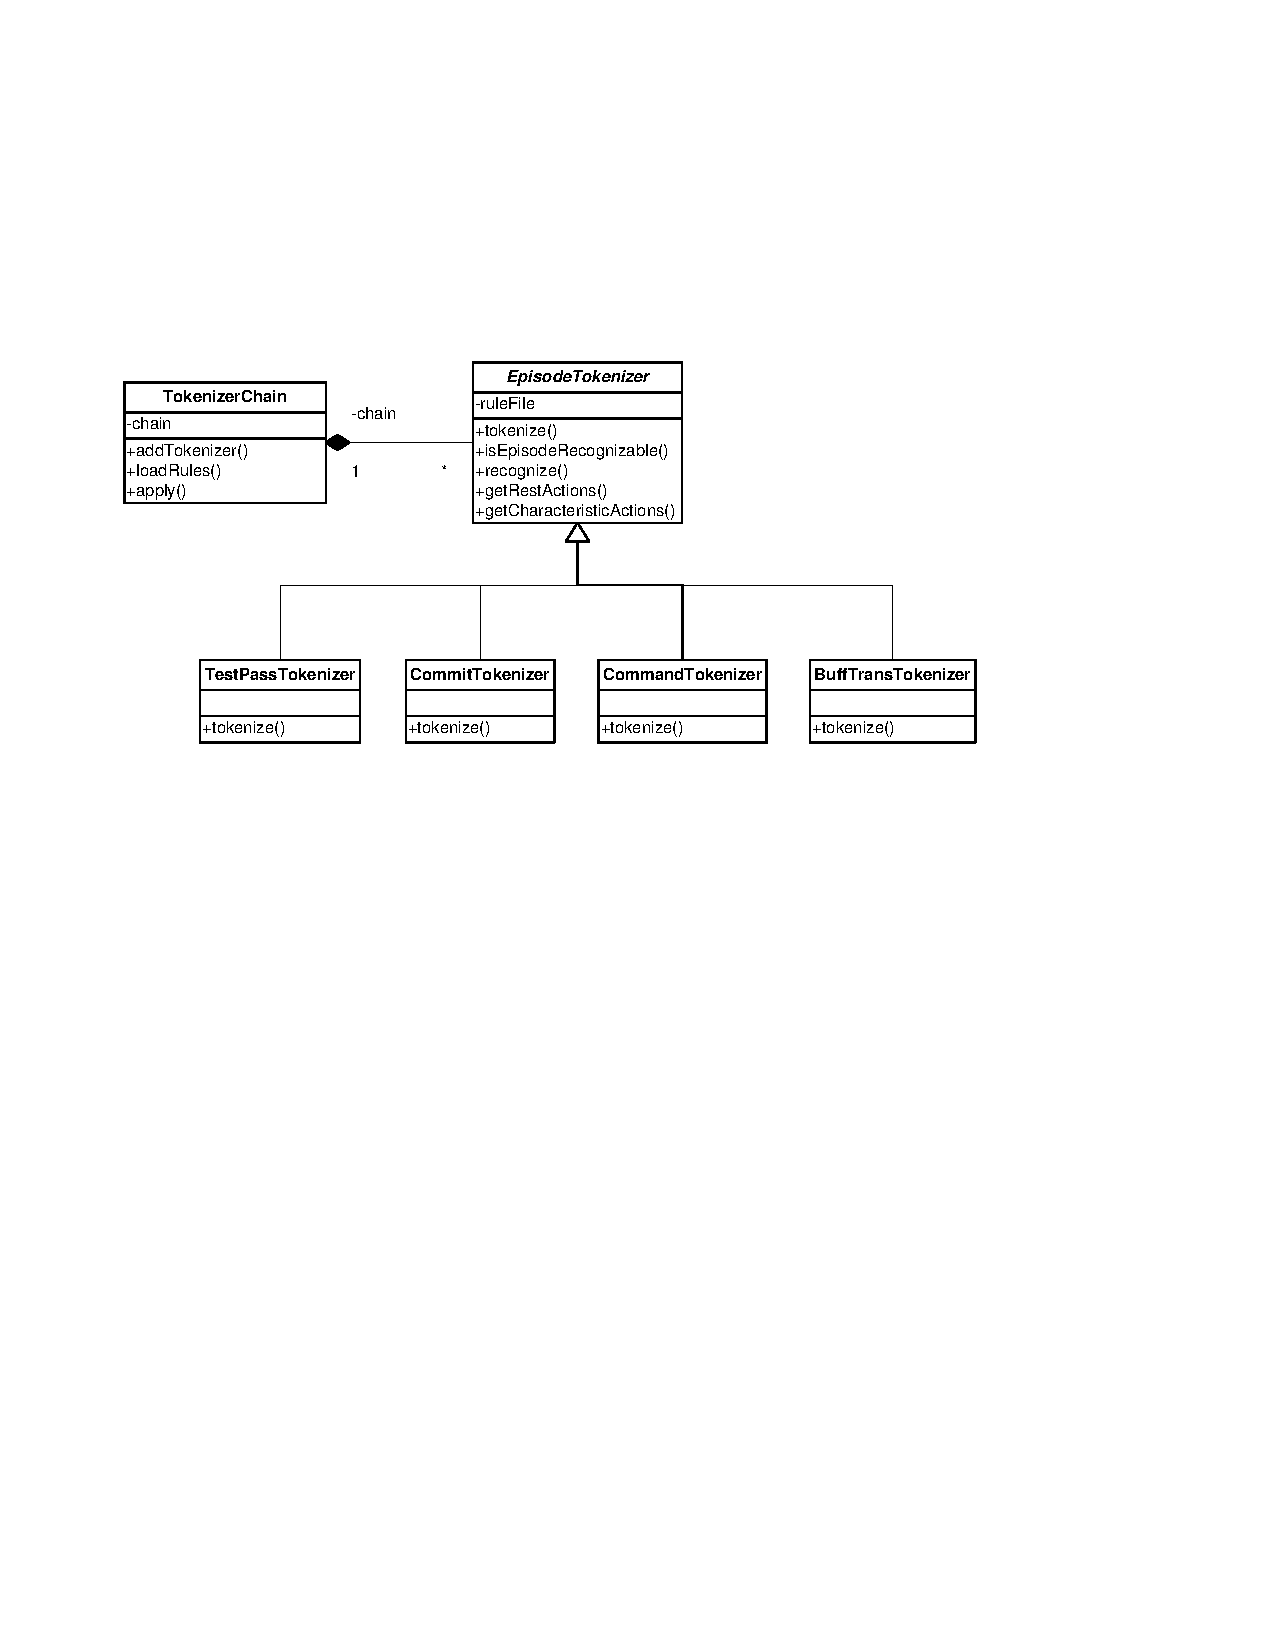
\includegraphics[width=0.8\textwidth]{figs/Visio-SDSA-Tokenizers-UML}
  \caption{Class Structure of SDSA Tokenizers}
  \label{fig:SDSA-Tokenizers}
\end{figure}

Although it is possible, it is not necessary to have multiple
tokenizers in a single run. In my dissertation research, I found that 
the ``test pass'' tokenizer is sufficient for the inference of 
Test-Driven Development behaviors.

% A software development stream could have thousands activities.
% It is hard to and time-consuming to analyeze a development stream
% which may have ton of activities. And, very likely, there is no
% any connection between a activity and another activities that is
% days or months away. So I decided to partition software 
% development streams. By using tokenizer, we may be able to cut
% them into chunks having activities that are clsey tied with
% each other. 
\subsection{Development Behaviors Inference}
\label{sec:SDSA-Inference}
SDSA infers development behaviors using JESS \cite{Friedman-Hill:03}, 
a rule-based system. Figure \ref{fig:SDSA-Inference} illustrates 
how SDSA interacts with JESS to infer development behaviors from
development actions in an episode. 
% regognition of Low-level Software Process Behaviors
% Utilize JESS, a rule-based system to look for and match
% the pattern of software development in episodes. 
\begin{figure}[htbp]
  \centering
  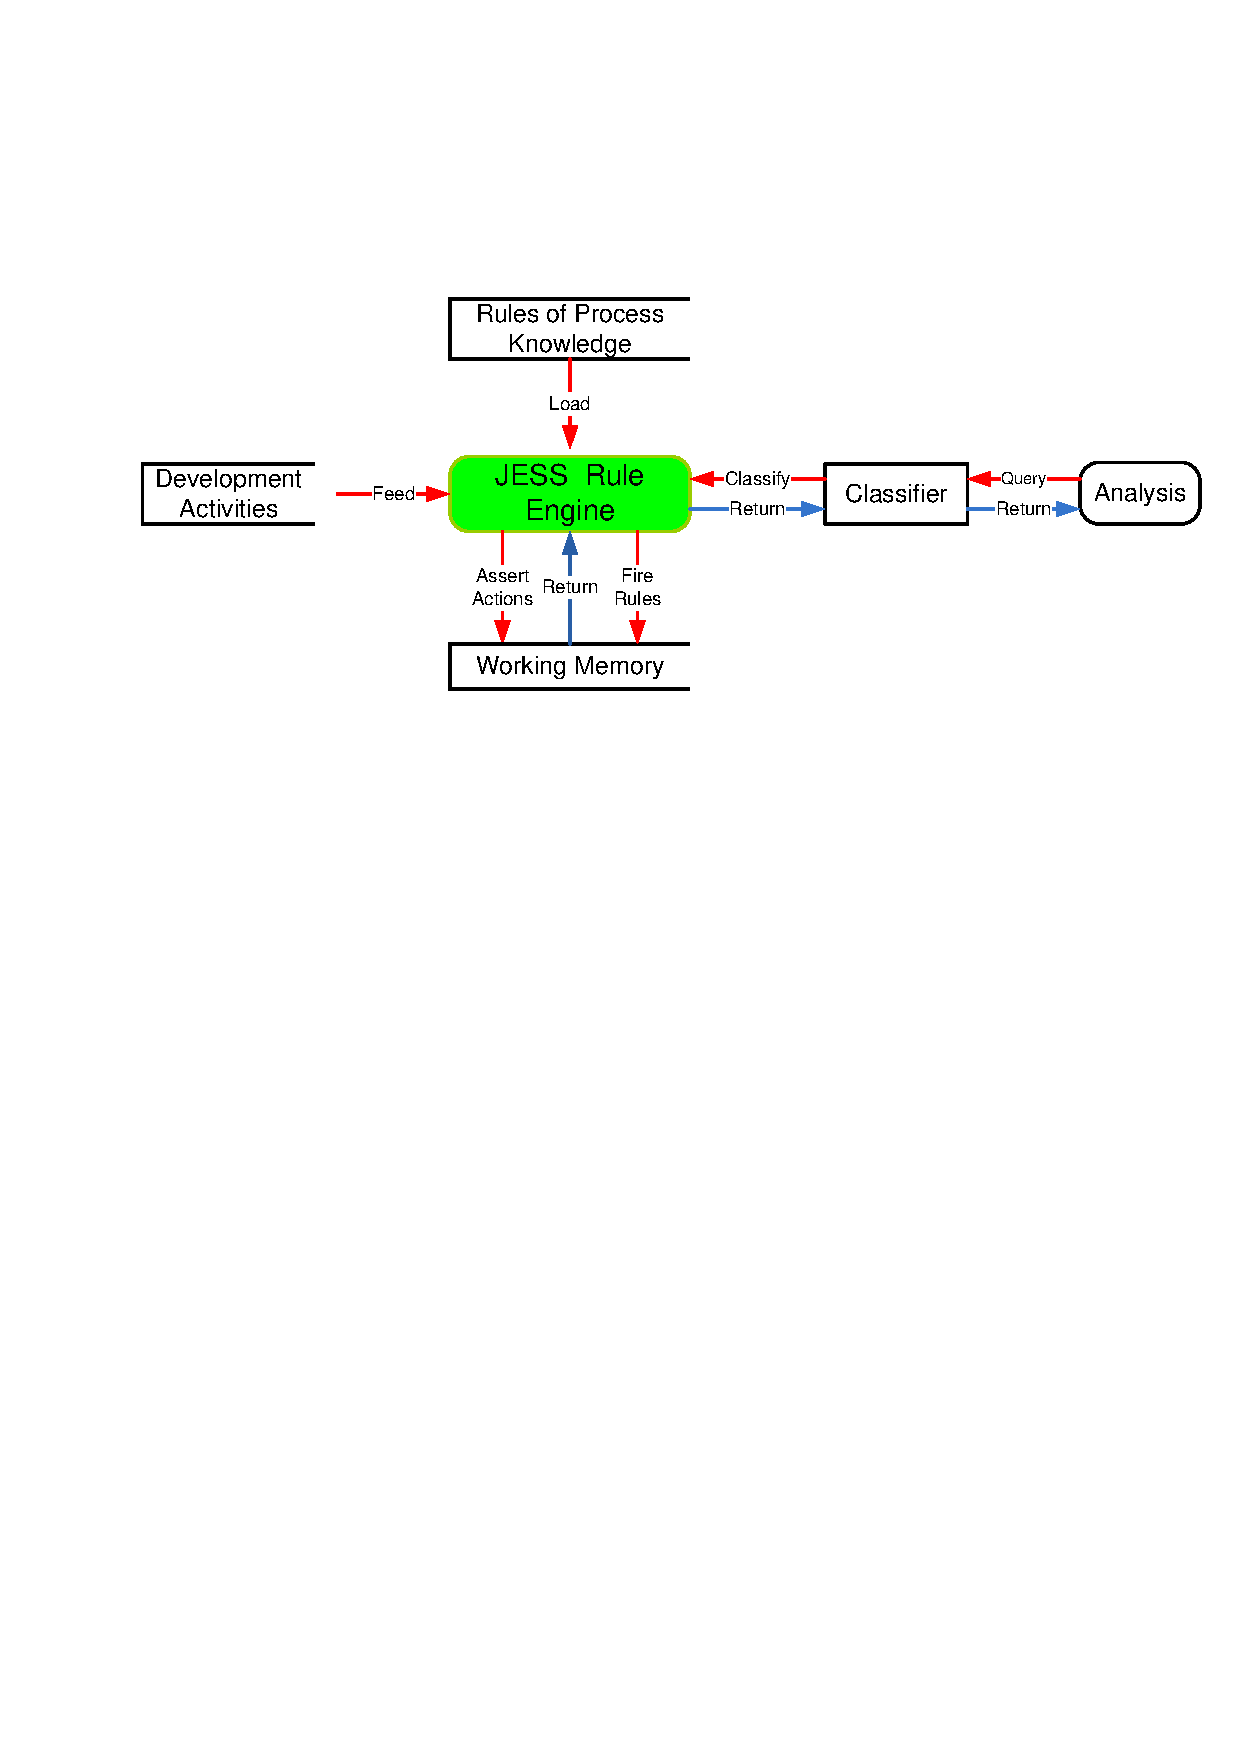
\includegraphics[width=1.0\textwidth]{figs/Visio-SDSA-BehaviorInference}
  \caption{Developer Behavior Inference}
  \label{fig:SDSA-Inference}
\end{figure}

The inference process is a mix of top-down and bottom-up 
methods. For the process of interest, developers can convert
the process knowledge into a set of rules, which are then fed 
into JESS's working memory. JESS can infer development behavior 
after all development actions in an episode are asserted in 
JESS as facts. Inferred results can be queried by applications 
via a classifier, the interface between JESS and SDSA.

\subsection{An Example}
\label{sec:SDSA-Example}
Now that we have shown how SDSA uses software process and 
product metrics for development behavior inference, I will 
use an example to demonstrate it. Figure \ref{fig:SDSA-Example} 
illustrates the usage of SDSA for inferring development behaviors. 
\begin{figure}[htbp]
  \centering
  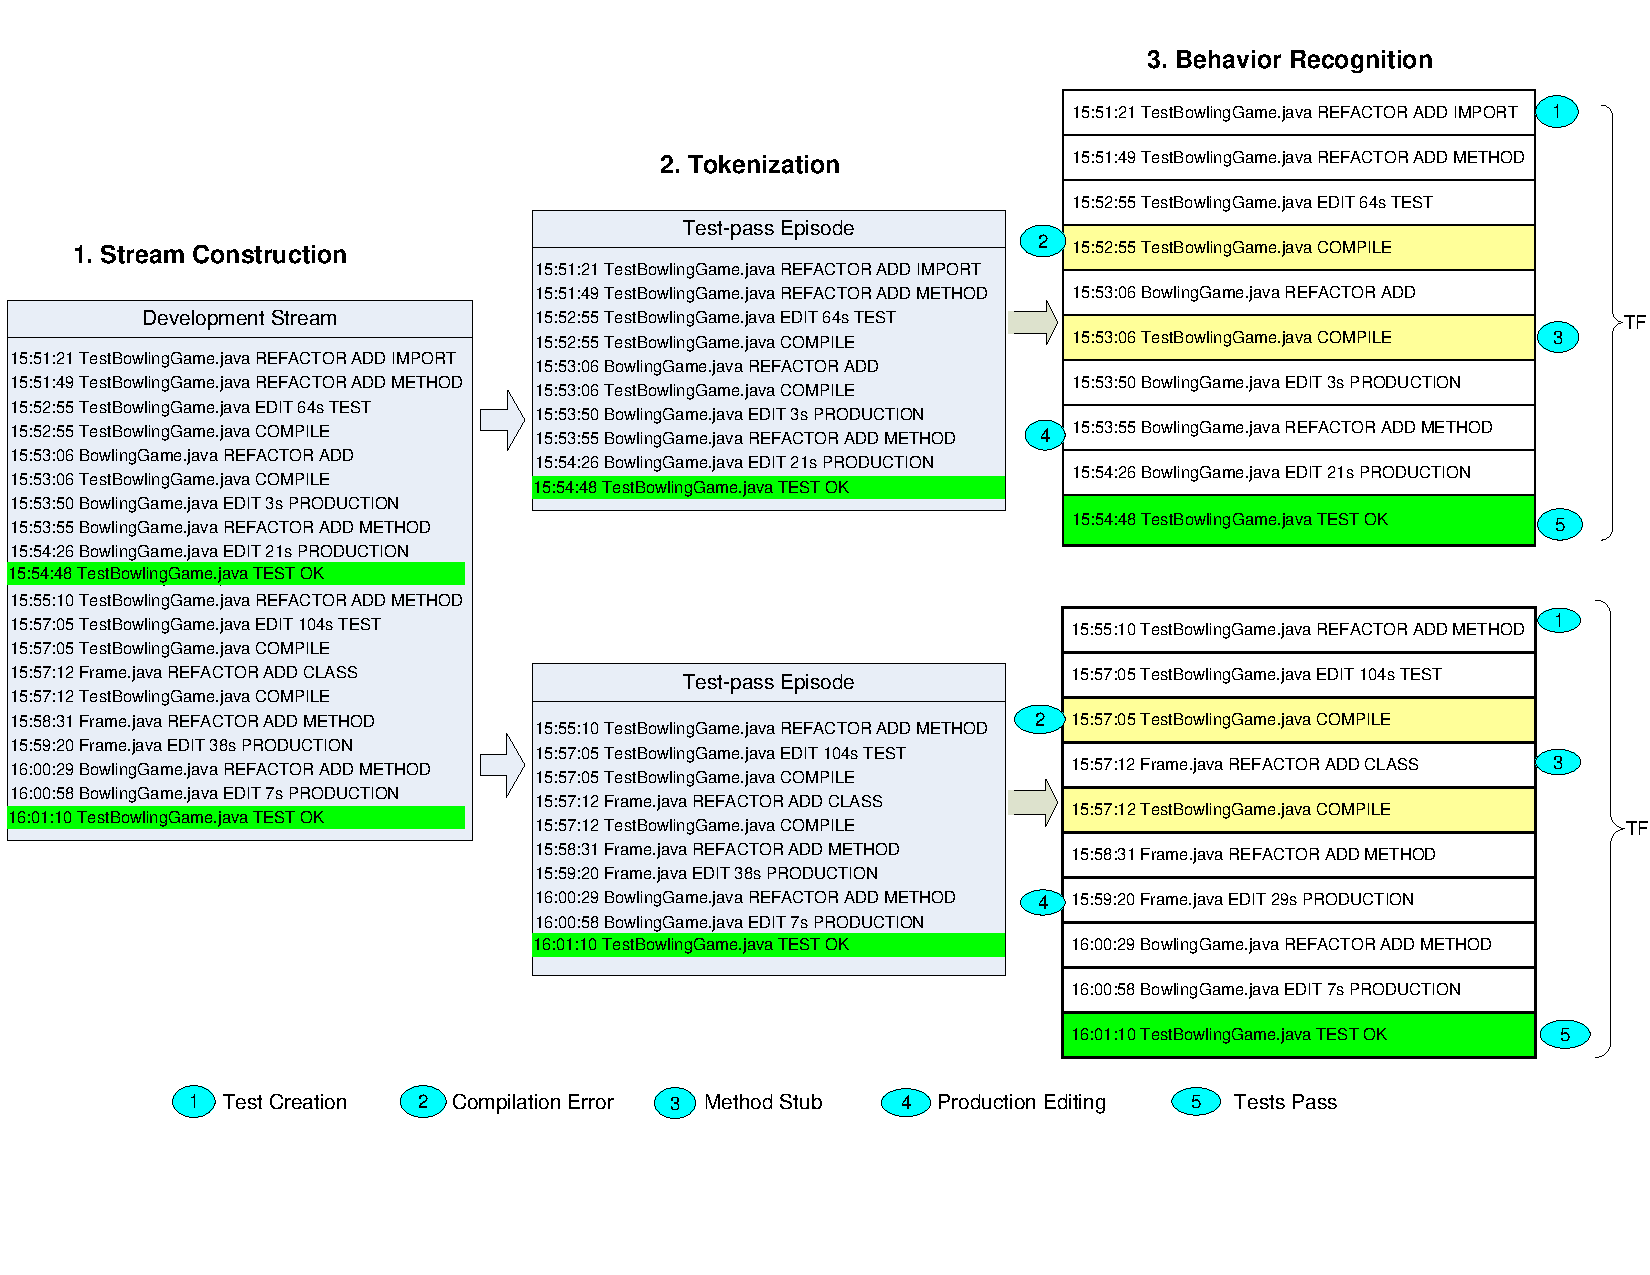
\includegraphics[width=1.0\textwidth]{figs/Visio-SDSA-Example}
  \caption{An SDSA Example}
  \label{fig:SDSA-Example}
\end{figure}
From 15:51:21 to 16:01:10, a developer implemented two user stories
of the bowling game in Test-Driven Development. We used Hackystat 
to instrument the development process and collected software process 
metrics including refactoring, editing, compilation and test 
invocations. Following the development stream construction method
described in Section \ref{sec:SDSA-Construction}, they were read 
and converted into development actions for construction of the
development stream. Part 1 of Figure \ref{fig:SDSA-Example} 
illustrates the internal structure of the development stream
that has 21 development actions. Among them, two are successful
test invocations that are painted in green background. Then, 
in part 2 of Figure \ref{fig:SDSA-Example}, SDSA's 
``Test Pass Tokenizer'' (See Section \ref{sec:SDSA-Partition}) 
was used to partition the development stream into two episodes. 
Further, development actions in the first episode were fed into
JESS to evaluate using an interface provided by SDSA. In part 3 
of Figure \ref{fig:SDSA-Example}, the inference rules detected 
a sequence of development activities that were in the order of 
(1) test creation, (2) compilation failures on test code, 
(3) method stub of production code, (4) production code editing, 
and (5) successful test invocation. Thus the development behavior 
in the first episode was recognized as ``TF'', a short name of 
Test-First. Similarly, the second episode was also recognized 
as ``TF'' by the inference rules.

%In this example, SDSA constructed a development stream on the 
%left-hand side, partitioned it into two episodes using the 
%``test pass'' tokenizer, and inferred that the development 
%behaviors in both episodes are a type of ``TF''. 

\section{Chapter Summary}
In this chapter, I first introduced Hackystat, a generic 
framework for software metrics collection and analyses, 
which makes it possible to design the SDSA framework for 
studying low-level software processes. SDSA has three 
sub-processes: (1) software development stream construction, 
(2) software development stream partition, and (3) 
development behavior inference. SDSA is configurable 
and extensible. I concluded this chapter with an example 
in Section \ref{sec:SDSA-Example} using a portion of a 
development stream developed in TDD. 
\chapter{Zorro Implementation}
\label{ch:Zorro}

With the capabilities provided by Hackystat and SDSA, as part of 
my dissertation research, I implemented the Zorro software system 
for the automation of Test-Driven Development (TDD) behavior 
inference. As illustrated in Figure \ref{fig:ZorroInfrastructure}, 
Zorro is a specialization of the SDSA framework for TDD, supported 
by Hackystat. Zorro not only uses Hackystat's generic services such 
as sensor data collection and persistence, but also contributes 
new functionalities to Hackystat. Zorro defines
several analyses and telemetry streams to study TDD using activities 
collected in development environment tools. This chapter starts with 
Zorro's extensions to the Hackystat and SDSA frameworks, followed 
by a collection of Zorro's TDD analyses.

\section{Extensions to Hackystat's Data Collection}
\label{sec:Zorro-Hackystat}

\begin{comment}
A nice thing about Hackystat is that numerous sensors have already 
been developed. Over two dozen sensors are currently available, including 
sensors for IDEs (Emacs, JBuilder, Eclipse, Vim, VisualStudio, Idea), 
configuration management (CVS, Subversion), testing and coverage (JUnit, 
CppUnit, Emma, JBlanket), and so forth. Though availability of tool 
supports gives developers the freedom to choose the right tool for 
a given task without losing process metric data, it is also difficult 
to automate the recognition. Thus, to begin with, Zorro requires that the TDD development 
must be done in a supported IDE. Under this premise, Zorro uses the 
sensor data collected in the IDE, and ignores other development activities
that are probably irrelevant to TDD. 
\end{comment}

Zorro has special requirements for Hackystat sensors that are 
responsible for collecting software metrics. In order to 
partition development streams and recognize TDD development 
behaviors, certain software development activities must be 
collected. Table \ref{tab:Zorro.Sensors} contains a list of the 
required development activities including edit, compile, test, 
switch file, and refactor. The ``DevEvent'' is 
a sensor data type defined in Hackystat to represent these 
kinds of development activities using the combination of ``Type'' 
and ``Subtype'' attributes. In addition, DevEvent defines a special 
attribute named ``PropertyMap'' to hold the required metrics, which 
are listed in the ``Product or Process Metrics'' column of 
Table \ref{tab:Zorro.Sensors}. Note that DevEvent does
not have the ``Kind'' attribute as you can see in 
Table \ref{tab:Zorro.Sensors}. It is for the sake of 
clarification for sensor developers to determine
what metrics are mandatory. For instance, if a test is
edited, the ``current-test-method'' and ``current-test-assertion'' 
metrics must be collected in addition to other metrics 
required for editing activities on production code. 

\begin{table}[htbp]
\centering
  \caption{Sensor Data Types Required by Zorro}
  \begin{tabular}{|p{2cm}|l|p{2.5cm}|l|p{6cm}|} \hline 
   Development & \multicolumn{2}{c|}{DevEvent} & \multicolumn{2}{c|}{Product or Process Metrics} \\ \cline{2-5}
   Activity & Type & Subtype & Kind & Names \\ \hline
   Edit &  Edit & StateChange and Save   & Document   & current-size \\ \cline{4-5}
        &       &                        & Production & current-size, class-name, 
                                                       current-methods, current-statements \\
                                                  \cline{4-5}
        &       &                        &  Test      & current-size, class-name, current-methods, 
                                                        current-statements, current-test-methods, 
                                                        current-test-assertions \\ \hline
   Compile     & Build    & Compile     &          &  success, error   \\ \hline   
   Test        & Test     & UnitTest    &          &  test-name, success, test-count, test-indice, 
                                                     elapsed-time, run-time \\ \hline 
   Switch File  & Edit   & BufferTransition &     & from-buff-name, to-buff-name \\ \hline                                                     
   Refactor    & Edit     & ProgramUnit & Unary    &  op (add or remove), unit-name, unit-type, 
                                                      language\\ \cline{4-5}
               &          &             & Binary   &  op (rename or move), unit-type, from-unit-name,
                                                      to-unit-name, language\\ \hline              
  \end{tabular}
  \label{tab:Zorro.Sensors}
\end{table}

These development activities are language and IDE independent. 
I wrote a sensor for Eclipse to gather these activities and more 
recently wrote a similar sensor for Visual Studio .NET. It 
should be possible to enhance a wide range of IDEs to collect 
necessary development activities for Zorro's automated TDD 
behavior inference.  

\section{Extensions to SDSA}
Zorro is a specialization of SDSA for automated inference of 
development behaviors of TDD. Figure \ref{fig:Zorro-SDSA-Workflow} 
illustrates how Zorro specializes SDSA. First, Zorro requires 
certain types of development activities, as described in 
Section \ref{sec:Zorro-Hackystat}. Thus, the development 
stream in Zorro is a special type of software development stream, which 
collects specific development activities useful for TDD recognition.
Second, Zorro uses the ``test pass'' tokenizer defined in the SDSA 
framework to partition the development stream. Last, a special set 
of rules are defined in Zorro to infer TDD development behaviors. In 
this section, I will describe Zorro's specialization of SDSA in detail.
\begin{figure}[htbp]
  \centering
  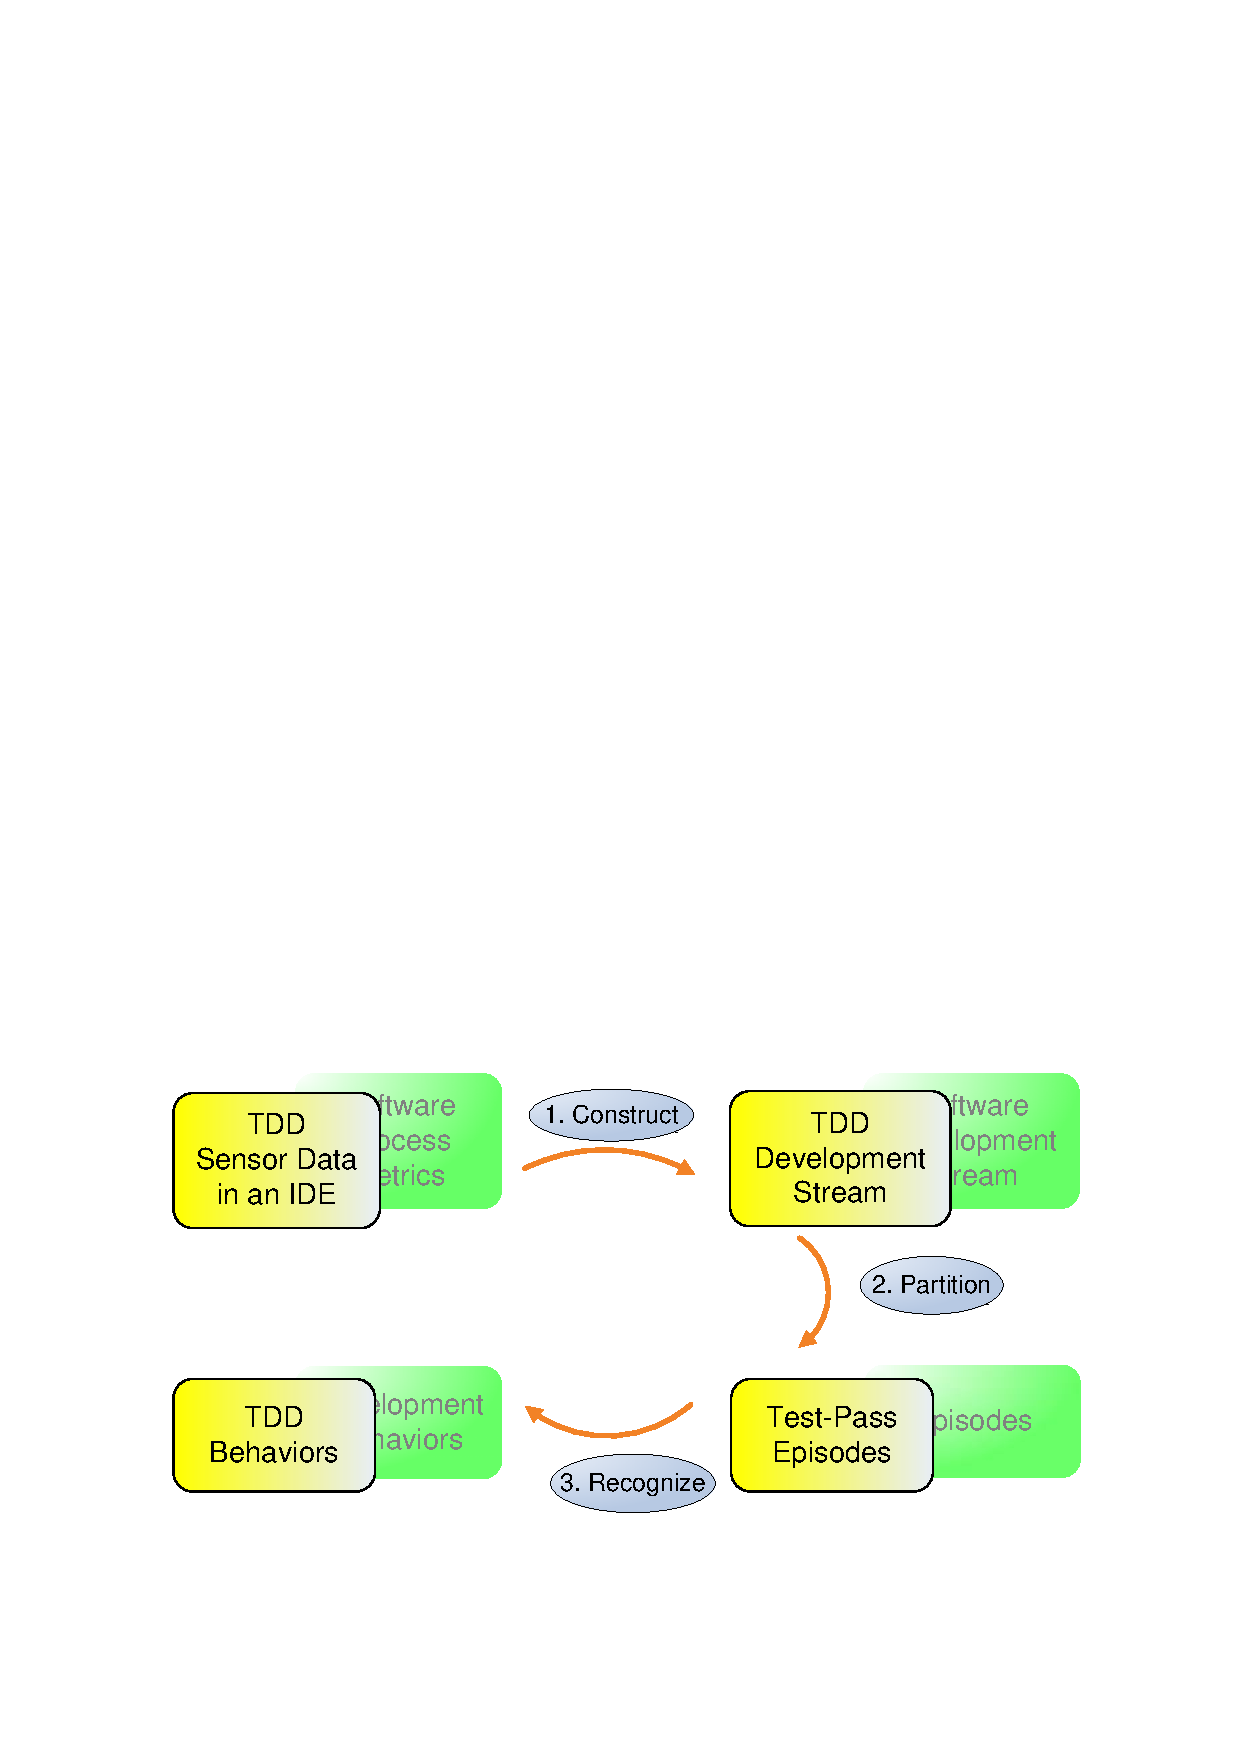
\includegraphics[width=0.8\textwidth]{figs/Visio-Zorro-SDSA-FlowChart}
  \caption{Zorro's Extensions to the SDSA Framework}
  \label{fig:Zorro-SDSA-Workflow}
\end{figure}

\subsection{Zorro Development Stream}
Edit, compile, test, switch file, and refactor are five types
of development activities required by Zorro. Though other 
development activities such as command line invocations can be 
conducted by developers, Zorro does not include them in
the development stream because they are not useful for 
recognition of TDD. The following code shows how Zorro 
constructs a development stream using SDSA. 
\begin{verbatim}
   DevelopmentStream stream = 
       new DevelopmentStream(project, user, startDay, endDay);
   stream.addSubstream(new EditStream(user));
   stream.addSubstream(new BuffTransStream(user));
   stream.addSubstream(new RefactoringStream(user));
   stream.addSubstream(new UnitTestStream(user));
   stream.addSubstream(new CompilationStream(user));
   stream.assemble(); 
\end{verbatim}
This piece of code instantiates a ``DevelopmentStream'' 
for a given project, a project member, and a specified time 
period indicated by the start day and the end day. It assembles
five action streams together to create the TDD development 
stream. 

\subsection{TDD Development Stream Partition}
Zorro uses the ``test pass'' tokenizer defined in the SDSA 
framework (see Section \ref{sec:SDSA-Construction}). As a 
result, a development stream is partitioned into a sequence 
of ``test pass'' episodes all of which end with successful 
unit test invocations. Figure \ref{fig:SDSA-Example} 
illustrates this process.

Before we move on, let's pause a while and think about the 
methods we are using. The development stream in Zorro 
contains five types of development activities that occur 
in an IDE when a developer is programming. These 
activities are not TDD specific. Moreover, the ``test
pass'' tokenizer is used to divide the TDD development stream
into ``test pass'' episodes. Again, the ``test pass'' tokenizer 
is not TDD specific and a developer might invoke tests no matter what
development methods he/she is using. Given this, how can we 
recognize development behaviors in TDD?  Can we use a dedicated 
tokenizer for TDD such as a ``TDD Iteration'' tokenizer? 

Recall that the order of programming in TDD is 
``Red/Green/Refactor''. If a developer programs in TDD, tests 
should be invoked one or more times. Given a task from the To-Do 
list (see Section \ref{sec:related-tdd}), a developer quickly 
writes a test and then invokes it. He or she will get a red
bar if the test fails. After implementing functional code 
for the task, he or she will invoke the test again to see it 
pass. Therefore, when the ``test pass'' tokenizer 
is used, we will get an episode containing the ``Red/Green'' 
development portion of a TDD cycle. If there is any redundancy
in the code, the developer will refactor it and then invoke
the test again. As a result, we will get another episode 
containing the ``Refactoring'' portion of a TDD cycle. If we 
can successfully recognize the ``test first'' behavior in the 
first episode and the ``refactoring'' behavior in the second 
episode, then we will be able to recognize TDD development 
behavior using the divide-conquer method. This shows that 
the ``test pass'' tokenizer is sufficient for recognition of 
development behaviors in TDD. The first question is answered. 

Can we have a ``TDD Iteration'' tokenizer? The answer is 
probably no. First, detecting refactoring development 
behaviors is hard. It is hard to tell whether a developer
is adding new code or refactoring for simpleness and clarification.
Second, as we have discussed in Chapter \ref{ch:Introduction}, 
developers may or may not conform to TDD, the Red/Green/Refactor 
cycle may not exist sometimes. Fortunately, the test pass tokenizer 
is sufficient for us to find the boundary of TDD's 
Red/Green/Refactor cycles as we just showed in last 
paragraph. 

\subsection{Inference of TDD Development Behavior}
\label{sec:ZorroBehaviorCategory}

%% Zorro use successful test invocations as the token to 
Zorro also extends SDSA with a set of rules that enable instances 
of test pass episodes to be classified as one of 22 episode types.  
Table \ref{tab:Zorro.Categories} lists these episode types,
their definition in terms of their internal patterns of
development activities, and an indication of their TDD 
conformance. 
\begin{sidewaystable}[htbp]
\centering
  \caption{Zorro episode types, definitions, and TDD conformance}
  \begin{tabular}{|l|p{18.5cm}|l|}
  \hline
   \textbf{ID}  & \textbf{Definition}   & \textbf{TDD Conformant} \\ \hline
   \multicolumn{3}{|l|}{\textbf{Test First}} \\ \hline
   TF-1 & Test creation $\rightarrow$ Test compilation error $\rightarrow$ 
          Code editing $\rightarrow$ Test failure $\rightarrow$ Code editing 
          $\rightarrow$ Test pass & Yes \\ \hline
   TF-2 & Test creation $\rightarrow$ Test compilation error $\rightarrow$ 
          Code editing $\rightarrow$ Test pass & Yes \\ \hline
   TF-3 & Test creation $\rightarrow$ Code editing $\rightarrow$ Test failure 
          $\rightarrow$ Code editing $\rightarrow$ Test pass    & Yes \\ \hline
   TF-4 & Test creation $\rightarrow$ Code editing $\rightarrow$ Test pass      
        & Yes \\ \hline

   \multicolumn{3}{|l|}{\textbf{Refactoring}} \\ \hline
   RF-1 & Test editing $\rightarrow$ Test pass  & Context sensitive \\ \hline
   RF-2 & Test refactoring operation $\rightarrow$ Test pass    & Context sensitive \\ \hline
   RF-3 & Code editing (number of methods or statements decrease) $\rightarrow$ Test pass       
        & Context sensitive \\ \hline
   RF-4 & Code refactoring operation $\rightarrow$ Test pass    & Context sensitive \\ \hline
   RF-5 & [Test Editing \&\& Code editing (number of methods or 
          statements decrease)]+ $\rightarrow$ Test pass        
        & Context sensitive \\ \hline
   
   \multicolumn{3}{|l|}{\textbf{Test Addition}} \\ \hline
    TA-1        & Test creation $\rightarrow$ Test pass & Context sensitive \\ \hline
    TA-2        & Test creation $\rightarrow$ Test failure $\rightarrow$ Test editing 
            $\rightarrow$ Test pass     
          & Context sensitive \\ \hline

   \multicolumn{3}{|l|}{\textbf{Regression}} \\ \hline
   RG-1 & Non-editing activities $\rightarrow$ Test pass        & Context sensitive \\ \hline
   RG-2 & Test failure $\rightarrow$ Non-editing activities $\rightarrow$ Test pass     
        & Context sensitive \\ \hline

   \multicolumn{3}{|l|}{\textbf{Code Production}} \\ \hline
    CP-1        & Code editing (number methods unchanged, statements increase) 
            $\rightarrow$ Test pass     
          & Context sensitive \\ \hline
    CP-2        & Code editing (number methods /statements increase slightly 
            (source code size increase $\leq$ 100 bytes) $\rightarrow$ Test pass        
          & Context sensitive \\ \hline
    CP-3        & Code editing (number methods /statements increase significantly 
            (source code size increase $>$ 100 bytes) $\rightarrow$ Test pass   
          & No \\ \hline

    \multicolumn{3}{|l|}{\textbf{Test Last}} \\ \hline
    TL-1        & Code editing $\rightarrow$ Test editing $\rightarrow$ Test pass       & No \\ \hline
    TL-2        & Code editing $\rightarrow$ Test editing $\rightarrow$ Test failure 
            $\rightarrow$ Test editing $\rightarrow$Test pass   
          & No \\ \hline

    \multicolumn{3}{|l|}{\textbf{Long}} \\ \hline
    LN-1        & Episode with many activities ($>$ 200) $\rightarrow$ Test pass        & No \\ \hline
    LN-2        & Episode with a long duration ($>$ 30 minutes) $\rightarrow$ Test pass & No \\ \hline

    \multicolumn{3}{|l|}{\textbf{Unknown}} \\ \hline
    UN-1        & None of the above $\rightarrow$ Test pass     & No \\ \hline
    UN-2        & None of the above     & No \\ \hline
  \end{tabular}
  \label{tab:Zorro.Categories}
\end{sidewaystable}

Zorro organizes the 22 episode types into eight categories: Test First
(TF), Refactoring (RF), Test Last (TL), Test Addition (TA), Regression
(RG), Code Production (CP), Long (LN), and Unknown (UN). All of these
episode types (except UN-2) always end with a ``Test Pass'' event, since 
that is the episode boundary condition.  UN-2 is provided as a way to 
classify a development stream where there is no unit testing at all.

\subsubsection{Test First}
``Test First'' can be seen as the Red/Green portion of a TDD cycle.
In a ``Test First'' episode, a test method or assertion statement is 
created first, followed by production code editing. Depending on 
compilation and test invocation results, an episode can be one of the
four types: TF-1, TF-2, TF-3, or TF-4, as illustrated in 
Table \ref{tab:Zorro.Categories}. 

\subsubsection{Refactoring}
Refactoring behaviors in reality are a bit complicated to recognize 
automatically because developers can refactor code in many different 
ways. A simple scenario of refactoring is to change a method implementation 
without changing its input and output. To accomplish this, the developer 
can edit code directly or abstract a new method from it for reuse. 
Directly matching the patterns of refactoring behaviors is hard, but 
we can observe them indirectly. 
First of all, there should be no test created. Second, code being 
refactored should not increase in size. If it does, the increase 
should be relatively small. With these two principles in mind, we can define
rules to infer refactoring behaviors. Table \ref{tab:Zorro.Categories}
lists five kinds of refactoring episodes: RF-1, RF-2, RF-3, RF-4, and 
RF-5. Among them, RF-1 and RF-2 are refactoring on test, RF-3 and RF-4 
are refactoring on production code, and RF-5 defines mixed refactoring 
on both test and production code. 

\subsubsection{Test Addition}
If you are a TDD developer, you probably have never heard of ``Test Addition''
since Beck did not explicitly define it in \cite{Beck:03}. However,
you may occasionally add a test that does not drive implementation of
new production code, thus ``Test Addition'' exists even if you do not
realize it. It is fundamentally different from the refactoring behavior 
on test code because test methods and assertion statements are added. 
Zorro defines two types of ``Test Addition'' behaviors: TA-1 and TA-2.

\subsubsection{Regression}
It is always a good habit to run existing tests before adding any new 
code into the system, especially at the beginning. This development behavior
is called the regression test. The tests may fail due to problems such 
as incorrect environment settings, so the regression behavior has two 
categories: RG-1 and RG-2. 

\subsubsection{Code Production}
Recall that developers might not develop software 
following the pattern of Red/Green/Refactor all the time, as we discussed
in Chapter \ref{ch:Introduction}. Also, some developers may use 
other software development methods, such as Test Last Programming. 
For example, it is possible that a big chunk of production code can be inserted 
into the system without corresponding tests. Although tests
are invoked in the end, the development behavior is actually about 
writing production code. Zorro therefore defines ``Code Production'' to 
classify this variety of development behaviors. Depending on the size increase 
of production code, ``Code Production'' has three types: CP-1 (statement 
increase only), CP-2 (small code increase), and CP-3 (big production code 
increase).

\subsubsection{Test Last}
``Test Last'' is not a development behavior of TDD, but it is useful
to define it. Researchers have compared TDD to Test Last Programming or
Iterative Test Last \cite{Erdogmus:05,Matjaz:03}. If Zorro differentiates 
TDD from ``Test Last'', it can greatly help empirical researchers to study
TDD in practice.  ``Test First''  is opposed to ``Test Last'' where a test 
is created after production code implementation. ``Test Last'' has two
types: TL-1 and TL-2, however, the difference between the two types is 
very small. 

\subsubsection{Long}
Development behaviors in long episodes such as ones with too many 
development activities or ones that last a very long time (over 30 minutes)
are very hard to recognize. Therefore, Zorro does not infer development 
behaviors of long episodes. This is acceptable because iterations of TDD 
should be just seconds or minutes in duration\cite{Beck:01}. If an episode 
is very long, it is very likely not to be TDD conformant. 

\subsubsection{Unknown}
The last type of development behavior is ``Unknown''.
UN-2 is defined to classify development streams that do not have
any successful unit test invocation. UN-1 is defined to incorporate 
the situation that the rule set is insufficient, which is very rare but 
we can not exclude it. 

\subsection{TDD Conformance}
\label{sec:Zorro-TDDConformance}
% Two-way heuristic  
Once each episode instance has been assigned an episode type, the final 
step in the Zorro classification process is to determine the TDD 
conformance of that instance. Table \ref{tab:Zorro.Categories} shows 
that instances of some of the episode types are easy to characterize. 
For example, every instance of a ``Test First'' episode type is automatically 
TDD conformant, and every instance of a ``Test Last'', ``Long'' and 
``Unknown'' episode type is automatically not TDD conformant.

Interestingly, several of the episode types, such as ``Refactoring'', ``Test
Addition'', ``Regression'', and certain ``Code Production'' are ambiguous: in
certain contexts, they could be TDD conformant, while in others they could
be TDD non-conformant. This is because, for example, ``Refactoring'' can
legitimately occur while a developer is either doing TDD or some different 
development approach, such as Test Last Programming.  In
order to classify instances of these episode types, Zorro applies the
following heuristic: if a sequence of one or more ambiguous episodes are
bounded on both sides by TDD non-conformant episodes, then these ambiguous
episodes types are classified as TDD non-conformant.

To make this clear, let's consider some examples, such as the episode
sequence [TF-1, RF-1, CP-1, TF-2]. In this sequence, Zorro 
classifies the ambiguous episodes (RF-1 and CP-1) as TDD conformant, 
since they are surrounded by TDD conformant episode types (TF-1 and TF-2). 
Figure \ref{fig:Zorro-EpisodeSequence-ExampleA} illustrates this scenario.  
In Figure \ref{fig:Zorro-EpisodeSequence-ExampleA}, a rectangle with 
letters represents an episode, and it is painted with green background 
if it is TDD conformant according to the heuristic. 
\begin{figure}[htbp]
  \centering
  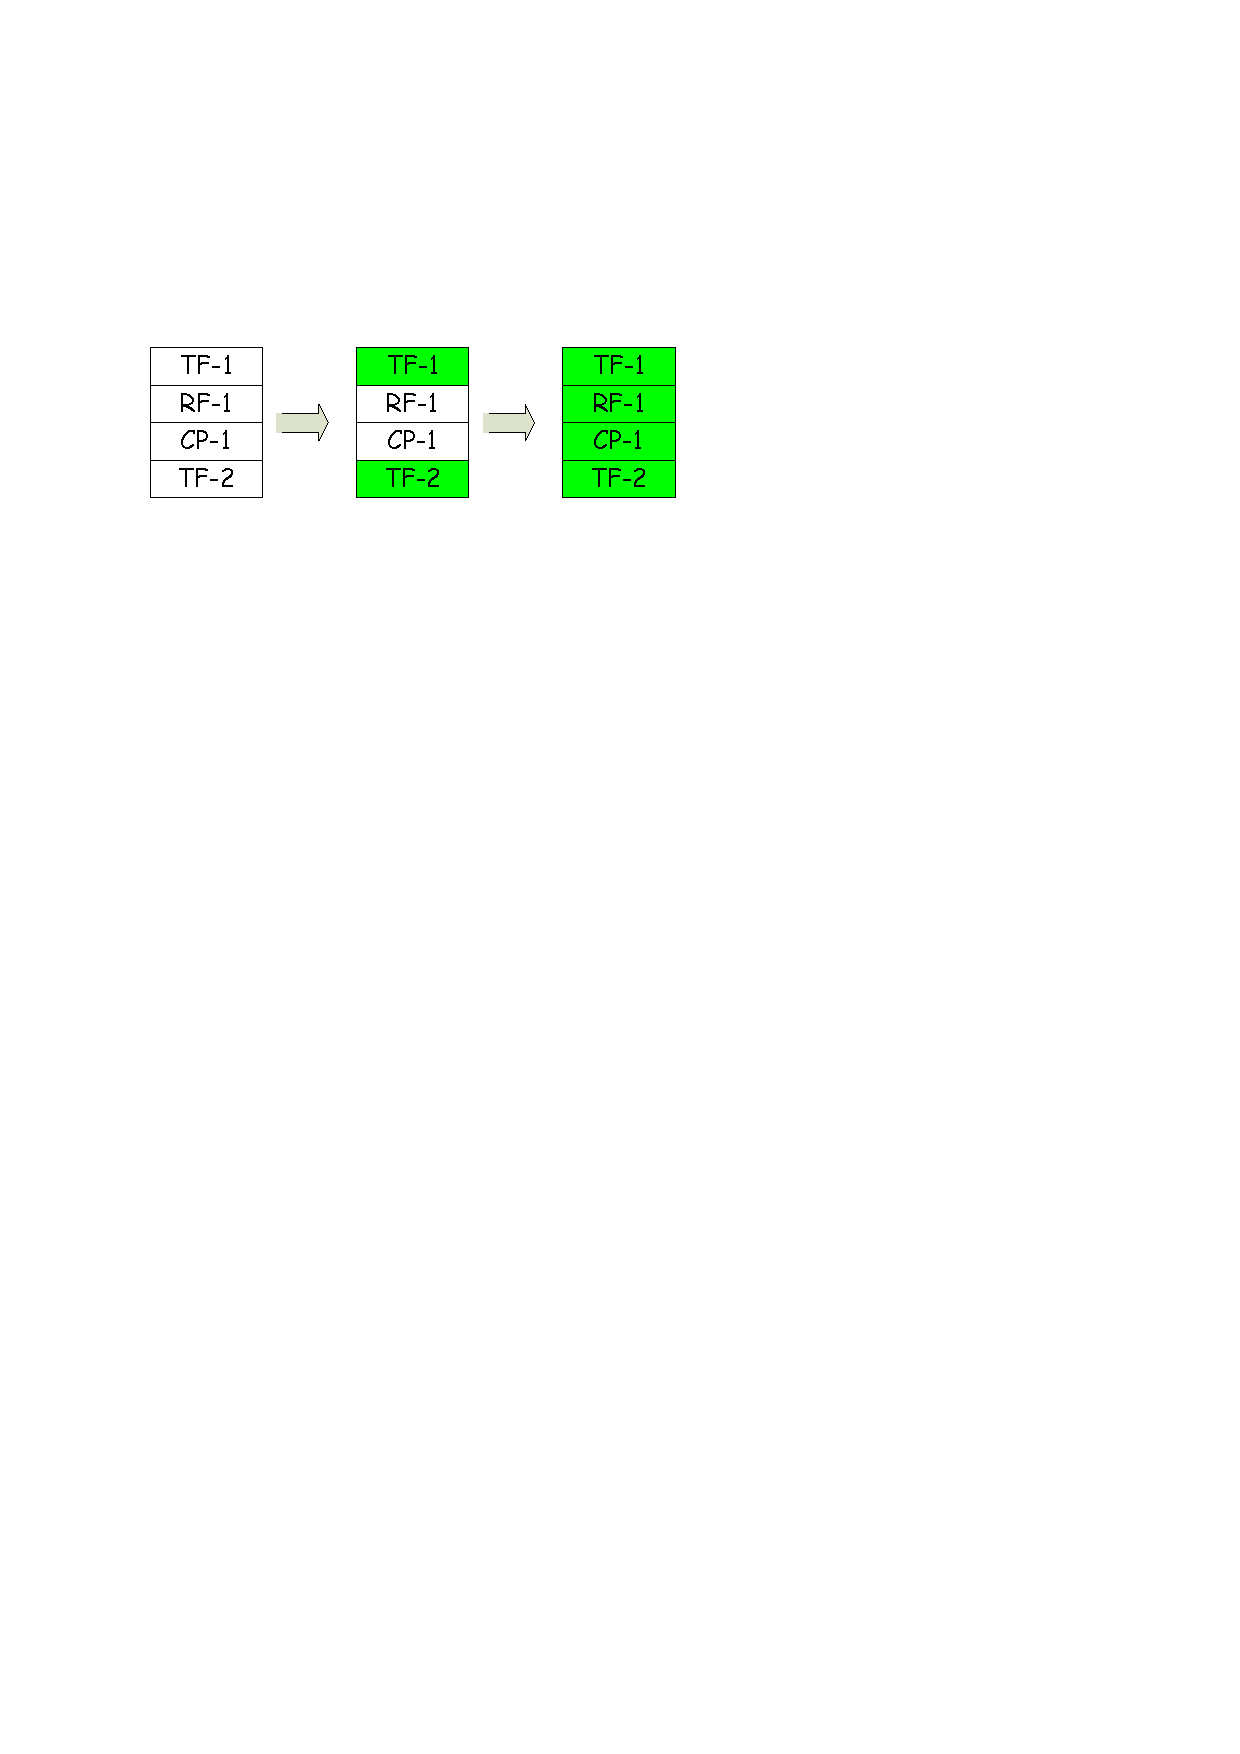
\includegraphics[width=0.4\textwidth]{figs/Visio-Zorro-Heuristic-Example1}
  \caption{Episode Sequence Example A}
  \label{fig:Zorro-EpisodeSequence-ExampleA}
\end{figure}

Now consider the sequence: [TL-1, RF-1, CP-1, TL-2].  In this sequence, 
Zorro classifies the same two ambiguous episodes (RF-1 and CP-1) as TDD 
non-conformant, since they are surrounded by TDD non-conformant episode types 
(TL-1 and TL-2). This scenario is illustrated in Figure 
\ref{fig:Zorro-EpisodeSequence-ExampleB} where an episode is painted
with red background if it is TDD non-conformant. 
\begin{figure}[htbp]
  \centering
  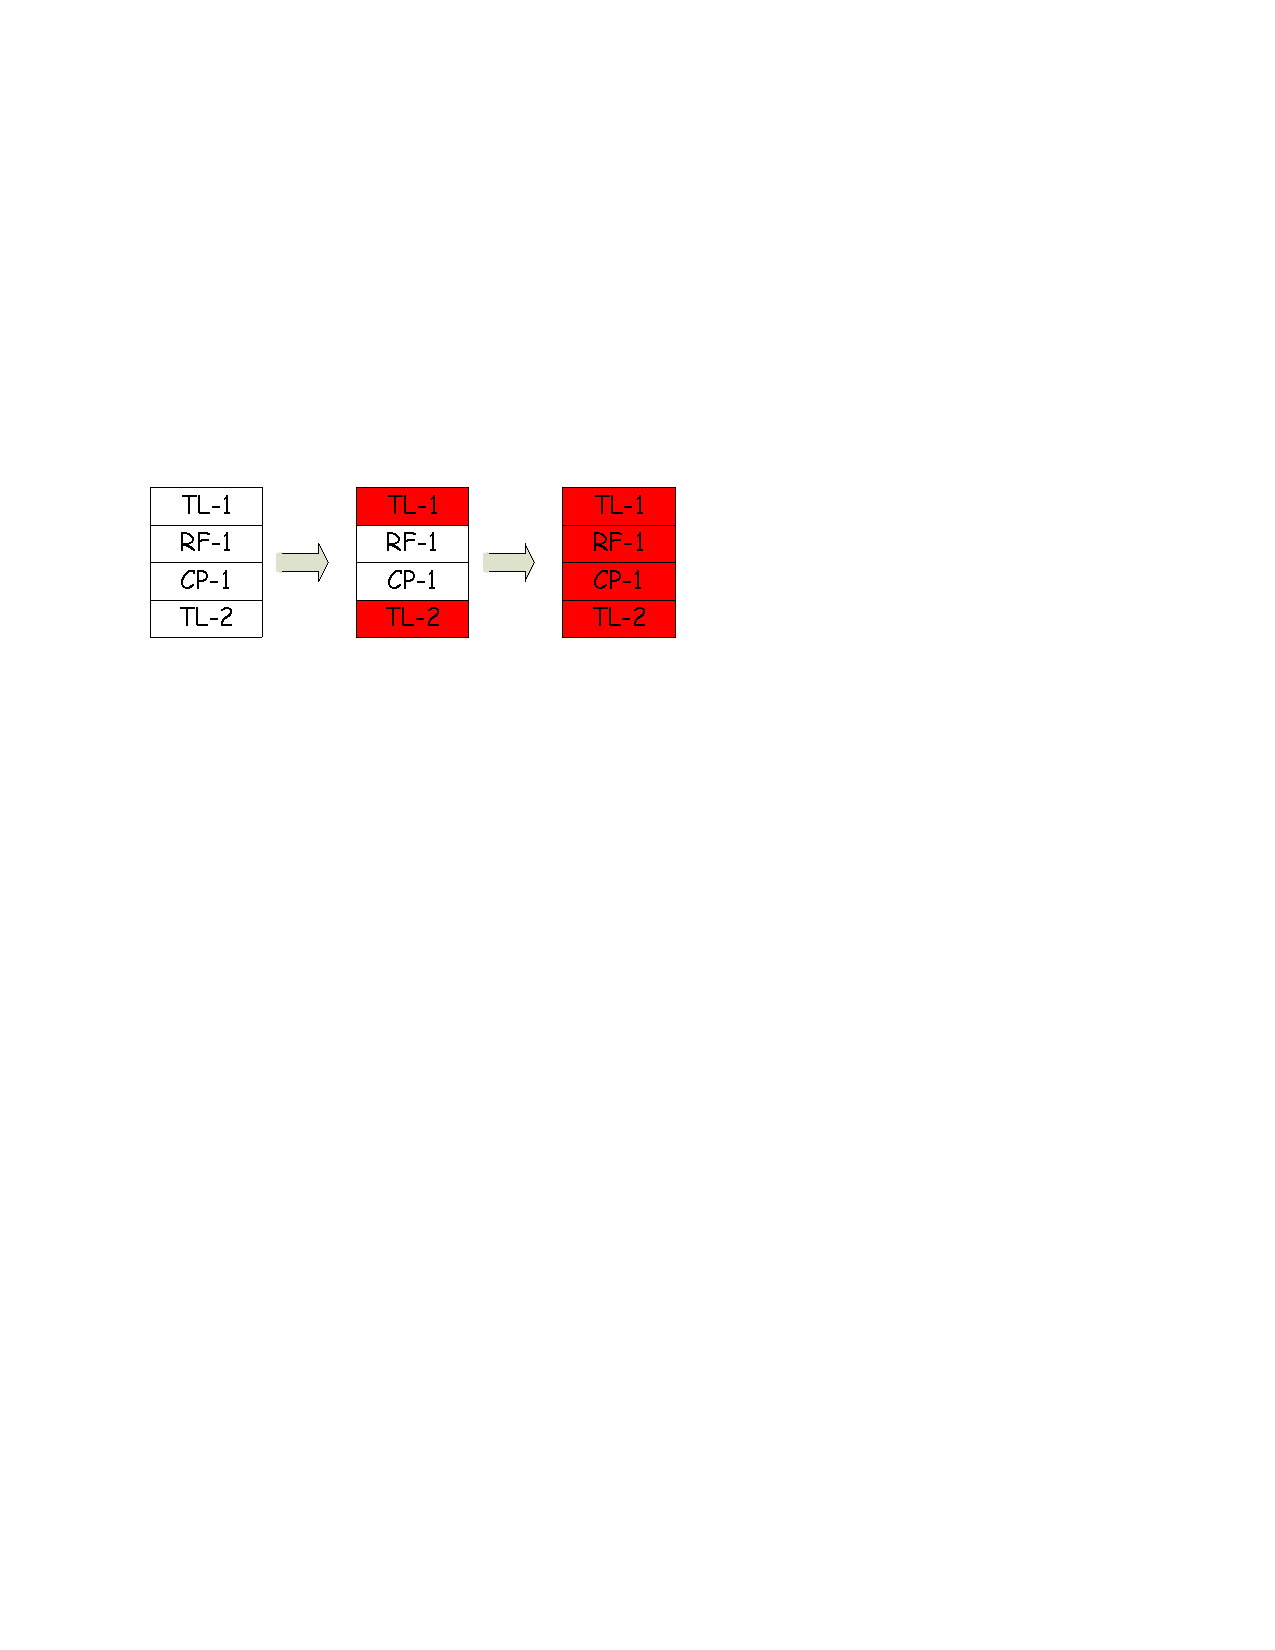
\includegraphics[width=0.4\textwidth]{figs/Visio-Zorro-Heuristic-Example2}
  \caption{Episode Sequence Example B}
  \label{fig:Zorro-EpisodeSequence-ExampleB}
\end{figure}

Now consider a sequence like: [TL-1, RF-1, CP-1, TF-1] illustrated 
in Figure \ref{fig:Zorro-HeuristicAlgorithm}. Here, the two ambiguous 
episodes (RF-1 and CP-1) are surrounded on one side by an unambiguously 
TDD conformant episode (TL-1) and on the other side by an unambiguously 
TDD non-conformant episode (TF-1).  In this case, Zorro's rules 
could implement an ``optimistic'' classification, and assign the
ambiguous episodes as TDD, or a ``pessimistic'' classification, and 
assign the ambiguous episodes as TDD non-conformant. 
Figure \ref{fig:Zorro-HeuristicAlgorithm} illustrates both of heuristics. 
\begin{figure}[htbp]
  \centering
  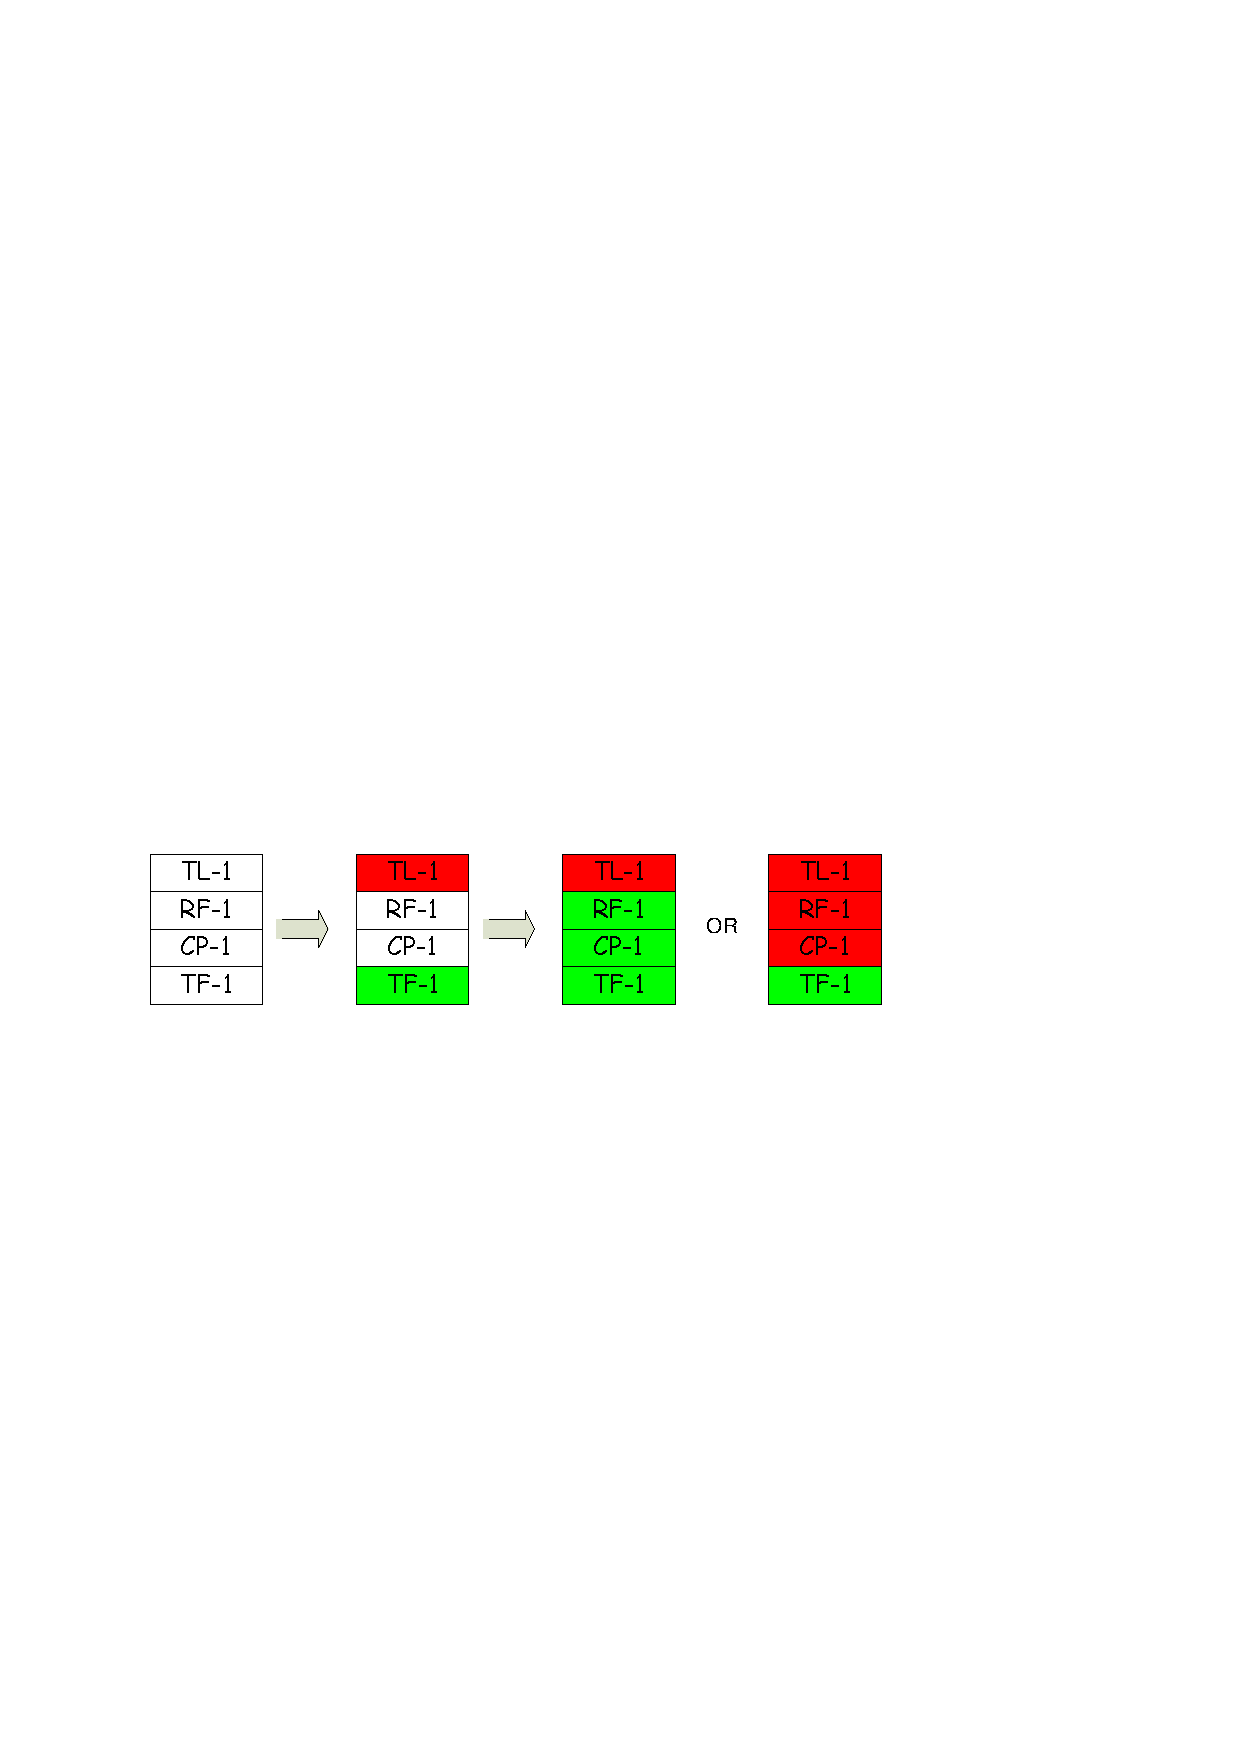
\includegraphics[width=0.6\textwidth]{figs/Visio-Zorro-Heuristic}
  \caption{Optimistic and Pessimistic Heuristic Algorithms}
  \label{fig:Zorro-HeuristicAlgorithm}
\end{figure}
Again, an episode is painted with green background if it is TDD 
conformant, otherwise it is painted with red background. Both of 
heuristics are supported by Zorro. In default, the optimistic
one is used, but Zorro allows developers to switch to the 
pessimistic heuristic.

\subsection{Zorro's TDD Episode Inference}
With episode categorization and TDD conformance heuristics, both 
of which are supported by the rule-based system, Zorro can automate
the recognition of TDD. 
%In addition, it can also differentiate TDD  from other development 
% methods, such as Test Last Programming. 
I conducted the ``TDD Episode Inference'' analysis using a real TDD 
development stream to demonstrate the Zorro's inference result. 
\begin{figure}[htbp]
  \centering
  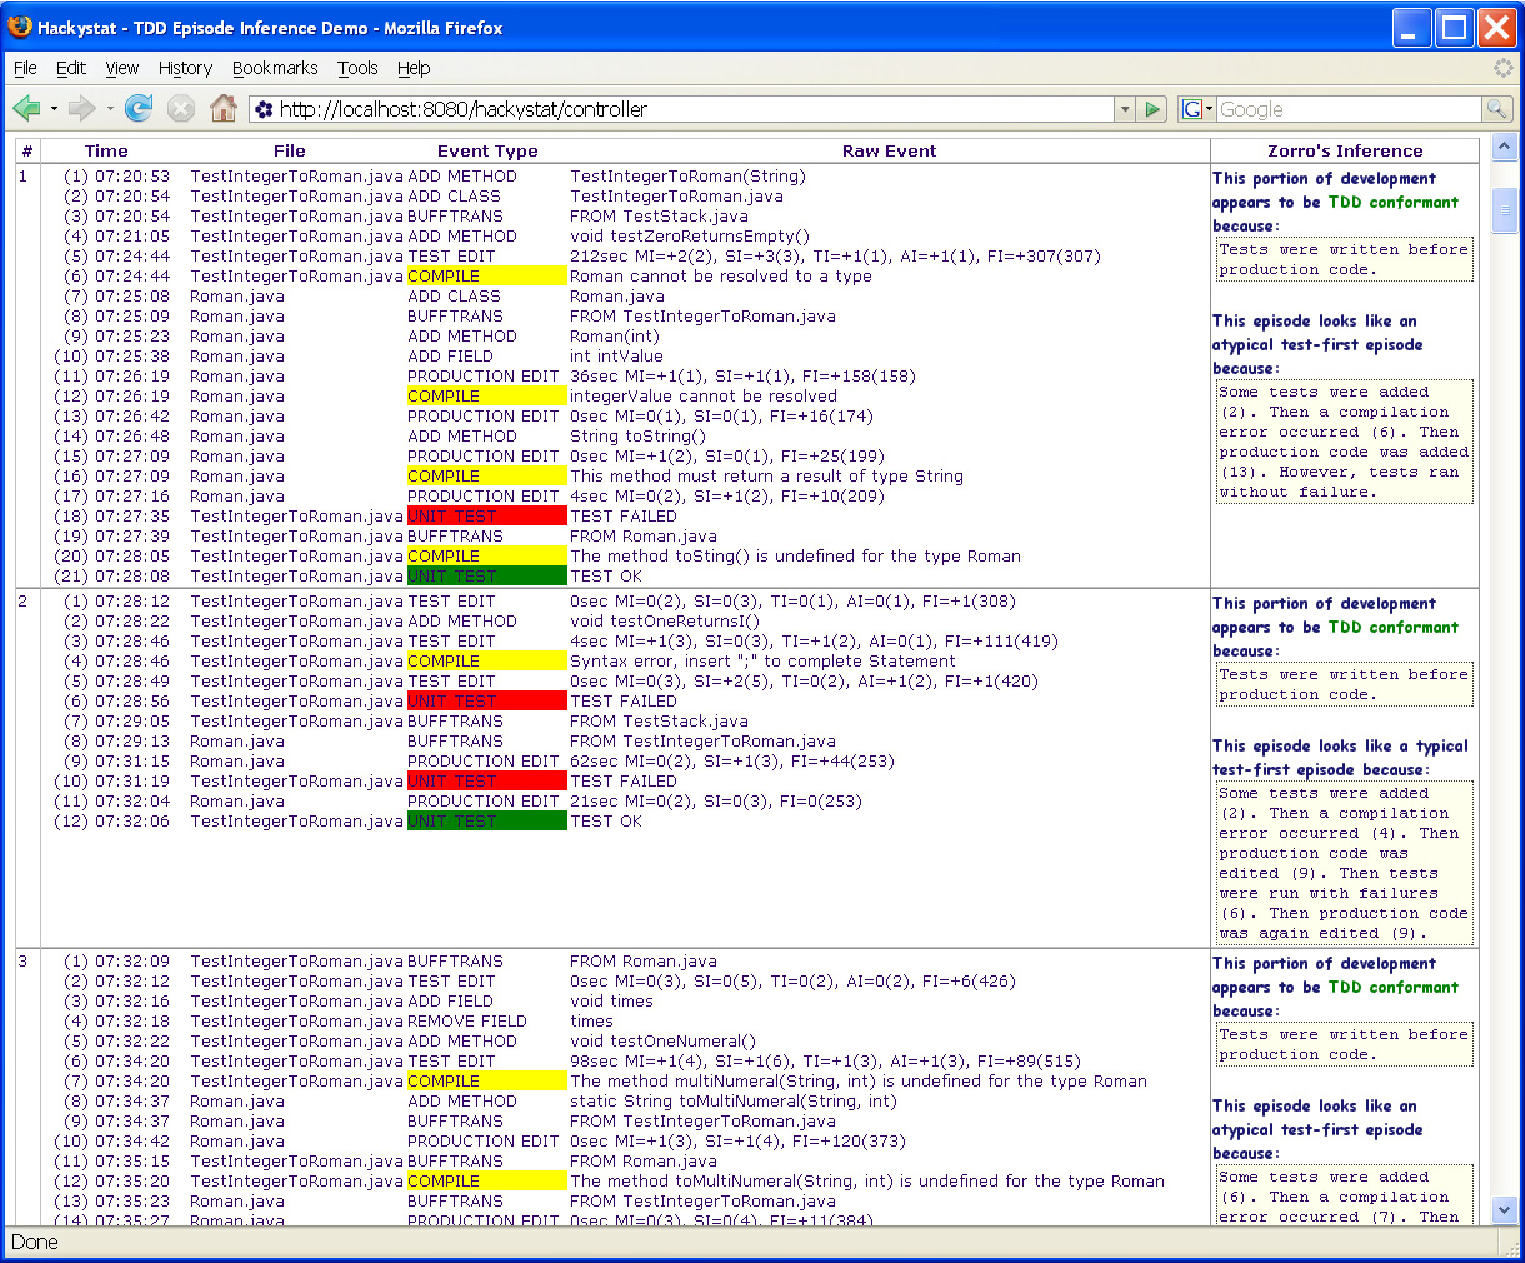
\includegraphics[width=0.9\textwidth]{figs/Zorro-Result-Demo}
  \caption{Demo of TDD Conformance Inference}
  \label{fig:Zorro-Process-Demo}
\end{figure}
An experienced developer solved the Roman numeral conversion problem 
(see Appendix \ref{app:UserStoriesRomanNumeral}) using TDD in the 
Eclipse IDE. The Hackystat Eclipse sensor was installed to instrument 
the development process for collecting development activities. Zorro 
partitioned his development stream into 16 episodes, and inferred 
his development behaviors. The screen-shot in 
Figure \ref{fig:Zorro-Process-Demo} shows the first three episodes 
with inferred development behaviors. They are all types of 
``Test First'' and conformant to TDD according to Zorro's inference.

This analysis is useful at demonstrating to new users how Zorro infers 
development behaviors. Another use of this analysis is 
to validate the correctness of Zorro's inference results. I will show 
how I enhanced this analysis for Zorro's validation in 
Chapter \ref{ch:Classroom}. Next, I will introduce Zorro's 
extensions to Hackystat's functionalities.

\section{Extensions to Hackystat's Functionalities}
TDD conformance is very important according to the discussion of related 
work in Chapter \ref{ch:RelatedWork}, and therefore I implemented 
the Zorro software system to provide explicit support for process 
conformance. Besides TDD conformance, 
with the capability of automated inference of TDD behaviors, more 
useful analyses that once were very hard can be conducted now. In 
the course of my research, I implemented TDD analyses including
``Episode Demography'', ``T/P Effort Ratio'', and 
``Episode Duration Distribution'' etc., for studying TDD 
(see Section \ref{sec:Zorro-Analysis}). Moreover, with the aid 
of Software project telemetry infrastructure, I implemented TDD 
telemetry reducers to assist research and management of software 
development in TDD (see Section \ref{sec:Zorro-Analysis-Telemetry}). 

\subsection{TDD Analyses}
\label{sec:Zorro-Analysis}
The following Zorro analyses have been developed to study software 
development in TDD and other development methods that include
unit testing.

% With our experiences, I have designed a set of analysis to understand
% an individual's practices of TDD. 
\subsubsection{Episode Demography}
The episode demography analysis provides an overview of a programming 
session as shown in Figure \ref{fig:Zorro-Analysis-EpisodeDemography}. 
\begin{figure}[htbp]
  \centering
  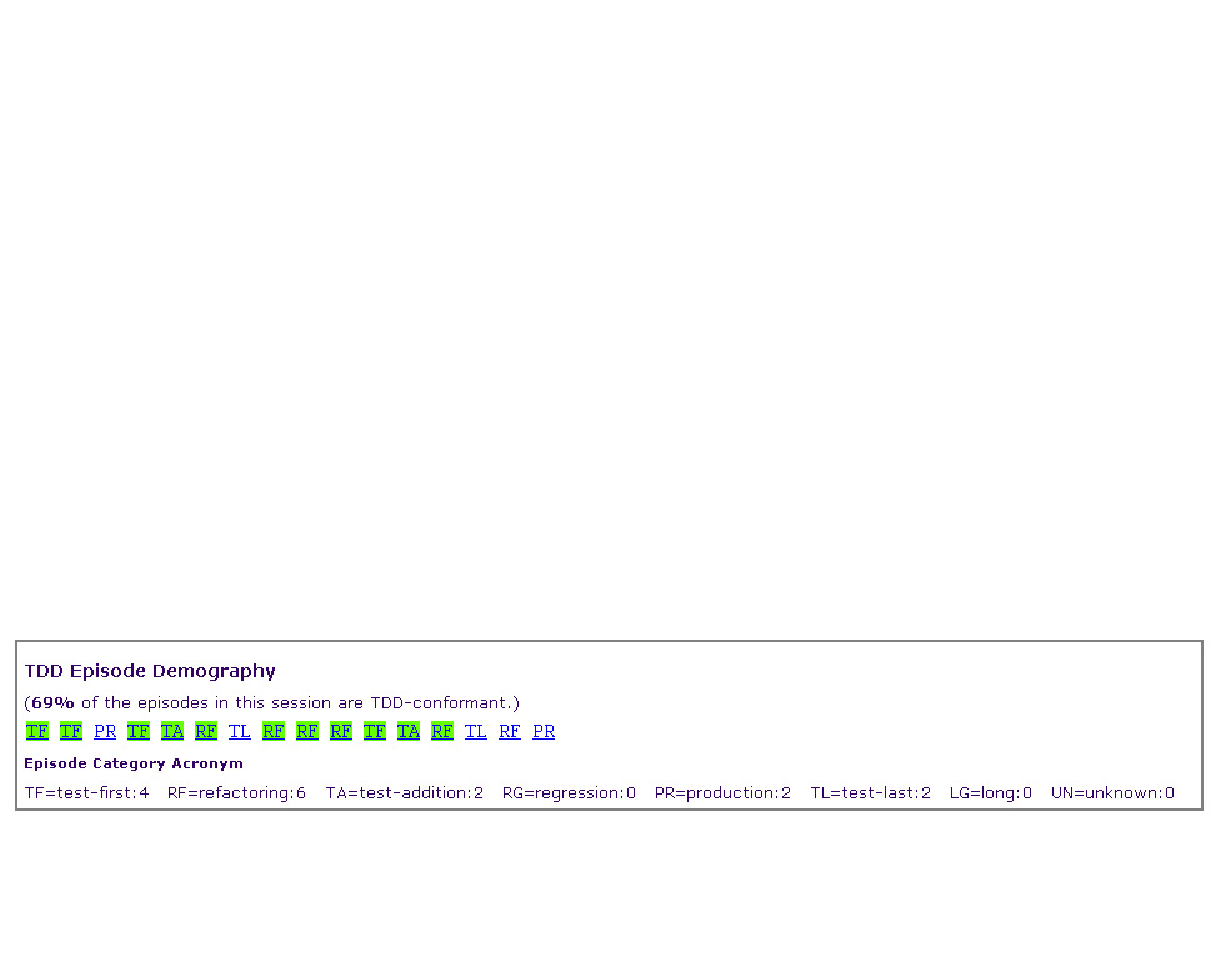
\includegraphics[width=1.0\textwidth]{figs/Zorro-Analysis-EpisodeDemography}
  \caption{Episode Demography Analysis}
  \label{fig:Zorro-Analysis-EpisodeDemography}
\end{figure}
In Figure \ref{fig:Zorro-Analysis-EpisodeDemography}, each small 
box with a two-letter acronym represents an episode. The legend
explains the links between two-letter episode acronyms and episode types. 
The background color of an episode tells its TDD conformance. 
If the episode is TDD conformant, the background is green; otherwise 
it is transparent. Episodes are clickable in the actual analysis. 
Clicking on an episode takes users to another analysis that is 
similar to the one illustrated in Figure \ref{fig:Zorro-Process-Demo}. 

Some useful information can be obtained using the episode demography
analysis. For instance, the example presented in Figure 
\ref{fig:Zorro-Analysis-EpisodeDemography} shows that this programming
session has 17 episodes, of which 69\% are TDD conformant. Four
episodes are ``Test First'', six are ``Refactoring'', and 
two are ``Test Last''. This information can be used to 
improve TDD conformance. If a higher degree of TDD conformance
is wanted, developers can study what are the legitimate TDD episodes 
to improve their compliance with TDD. Moreover, this analysis
can also be used to find development patterns. For instance, in
Figure \ref{fig:Zorro-Analysis-EpisodeDemography}, we can observe 
two patterns (TF)(TA)+ and (TA)(RF)+. The pattern (TF)(TA)+ means that 
a ``Test First'' episode is followed by one or more ``Test Addition''
episodes. The (TA)(RF)+ means that a ``Test Addition'' episode is 
followed by one or more ``Refactoring'' episodes.

\subsubsection{T/P Effort Ratio}
Unlike ``Episode Demography'', the ``T/P Effort Ratio'' analysis is not 
directly derived from Zorro's inference. In Section \ref{sec:Zorro-Hackystat},
we discussed that Zorro extends Hackystat's data collection. One 
extension is that it requires numbers of test methods and assertion 
statements. With this information, we can easily tell if a developer 
is working on test code at a given time. The T/P Effort
Ratio stands for the effort a developer spent on test code, 
compared to the effort spent on production code. 
Figure \ref{fig:Zorro-Analysis-TPEffortRatio} shows an example
of the T/P Effort Ratio analysis using the same TDD programming 
session used in Figure \ref{fig:Zorro-Analysis-EpisodeDemography}.
\begin{figure}[htbp]
  \centering
  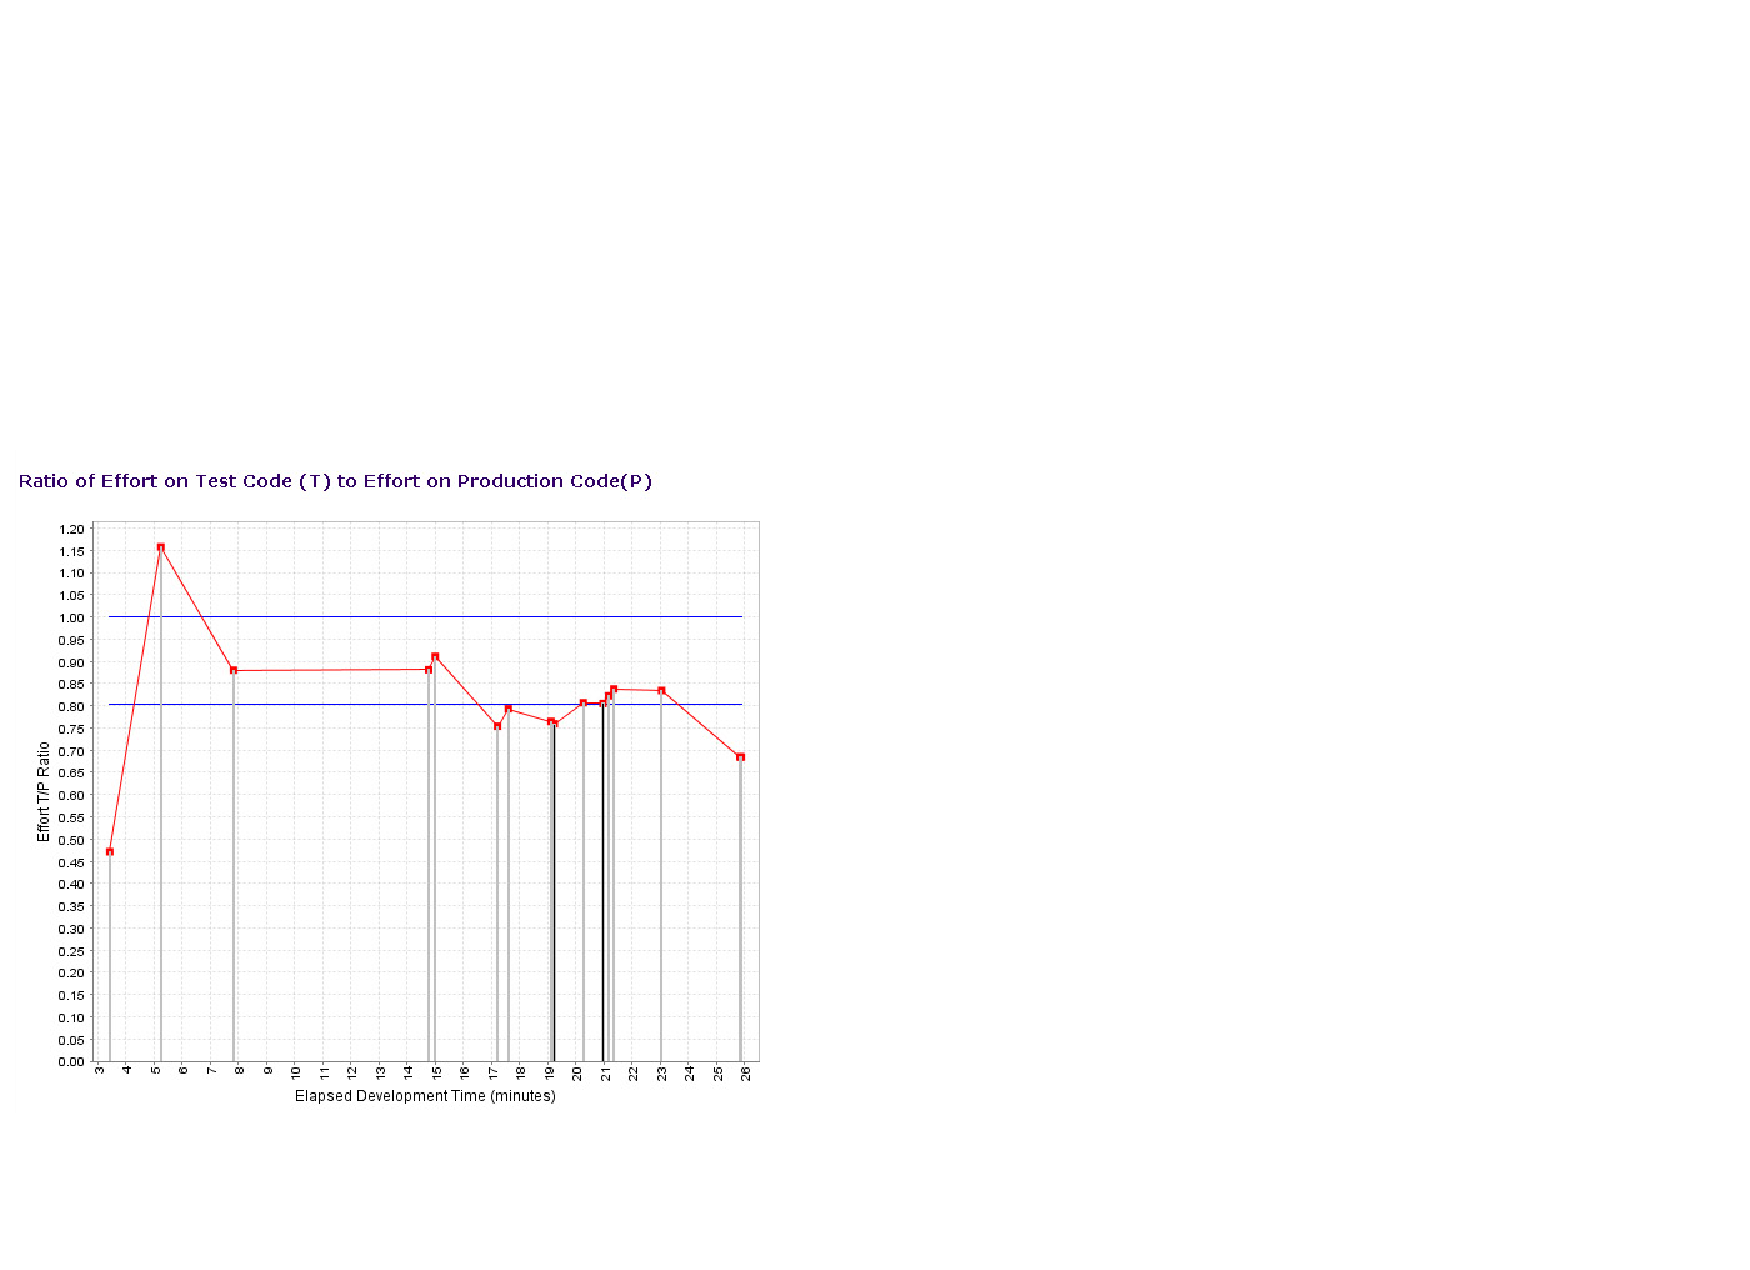
\includegraphics[width=0.7\textwidth]{figs/Zorro-Analysis-TPEffortRatio}
  \caption{Test Effort vs. Production Effort}
  \label{fig:Zorro-Analysis-TPEffortRatio}
\end{figure}
In Figure \ref{fig:Zorro-Analysis-TPEffortRatio}, the horizontal axis
is the elapsed development time in minutes, and the vertical axis is
the ratio of effort spent on test code to effort spent on production
code. The T/P ratio over 1.0 indicates more effort on writing
test code than on writing production code. The vertical bars are
episode borders, thus, the span between bars can represent episode 
durations.  

The example illustrated in Figure 
\ref{fig:Zorro-Analysis-TPEffortRatio} shows that the effort spent on
testing code is consistent over the course of this TDD development session. 
Approximately, on average, effort on testing code is about 80\% of effort
on production code. This analysis can be applied to not only TDD but also 
other development methods that include unit testing. An interesting use 
of it would be to compare T/P effort ratio differences between TDD and 
Test Last Programming. 

\subsubsection{T/P Size Ratio}
Same as the T/P Effort Ratio analysis, the T/P Size Ratio analysis is also
based upon Zorro's extension to Hackystat's data collection. In Table 
\ref{tab:Zorro.Sensors}, we have shown that the Zorro compatible sensor 
collects size information (current-size, mostly line of code) for both
of test and production code. With this information, we can compute the
incremental changes of test code size, production code size, and the 
ratio of the two. Figure \ref{fig:Zorro-Analysis-TPSizeRatio} shows 
an example of the T/P Size Ratio analysis using the same TDD programing 
session. 
\begin{figure}[htbp]
  \centering
  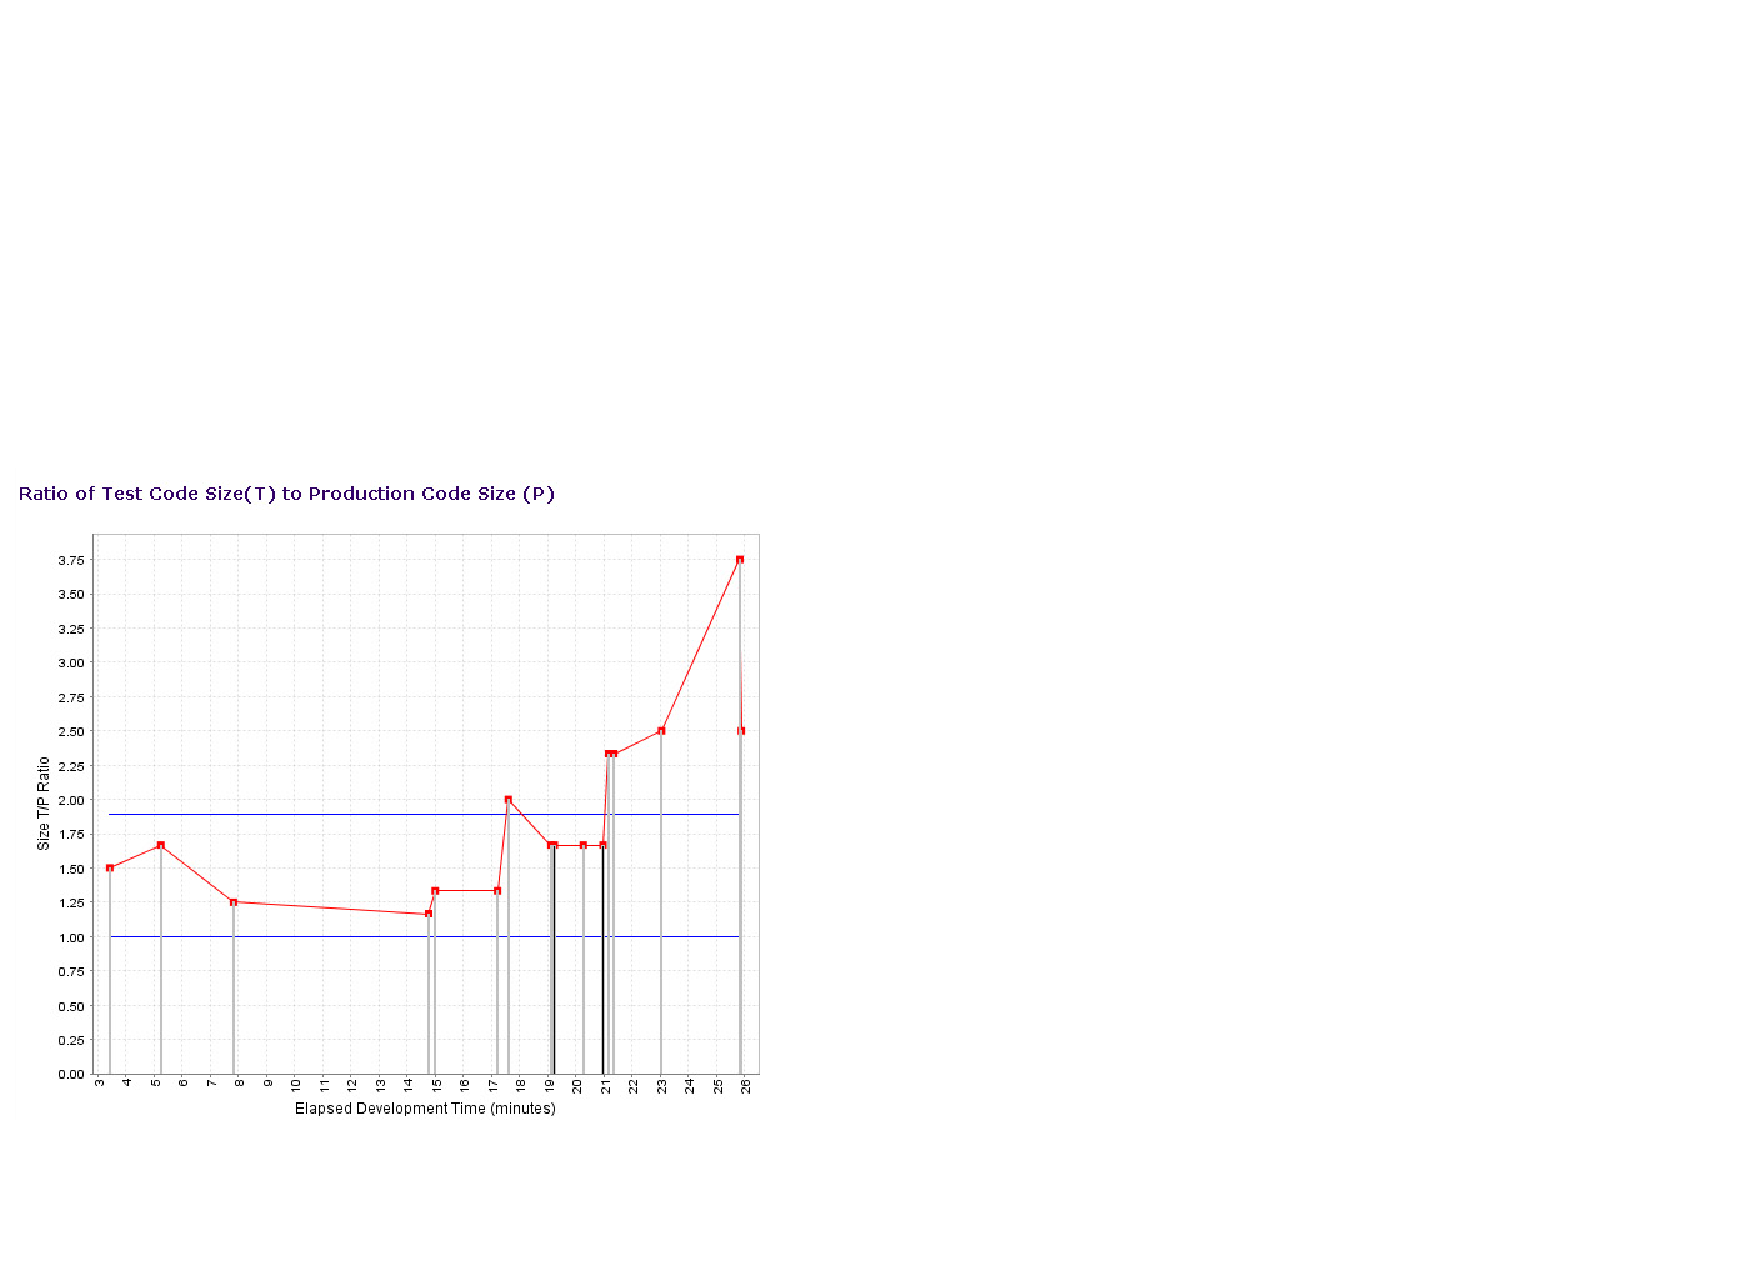
\includegraphics[width=0.7\textwidth]{figs/Zorro-Analysis-TPSizeRatio}
  \caption{Test Size vs. Production Size}
  \label{fig:Zorro-Analysis-TPSizeRatio}
\end{figure}
The interpretation to this analysis is exactly the same to Figure
\ref{fig:Zorro-Analysis-TPEffortRatio}, except that each value 
in Figure \ref{fig:Zorro-Analysis-TPSizeRatio} is the ratio of 
test code size to production code size. 

The example illustrated in Figure \ref{fig:Zorro-Analysis-TPSizeRatio}
shows that test code is always more than production code. Again, this
analysis is applicable to any development methods where unit testing 
is practiced. 

\subsubsection{Episode Duration}
The Episode Duration analysis is inspired by TDD's characteristically 
short durations that I discussed in Section \ref{sec:related-tdd}. How
frequently unit tests are invoked is an alternative indicator of 
TDD conformance \cite{Wang:04}. Figure \ref{fig:Zorro-Analysis-EpisodeDuration}
shows an example of the Episode Duration analysis. 
\begin{figure}[htbp]
  \centering
  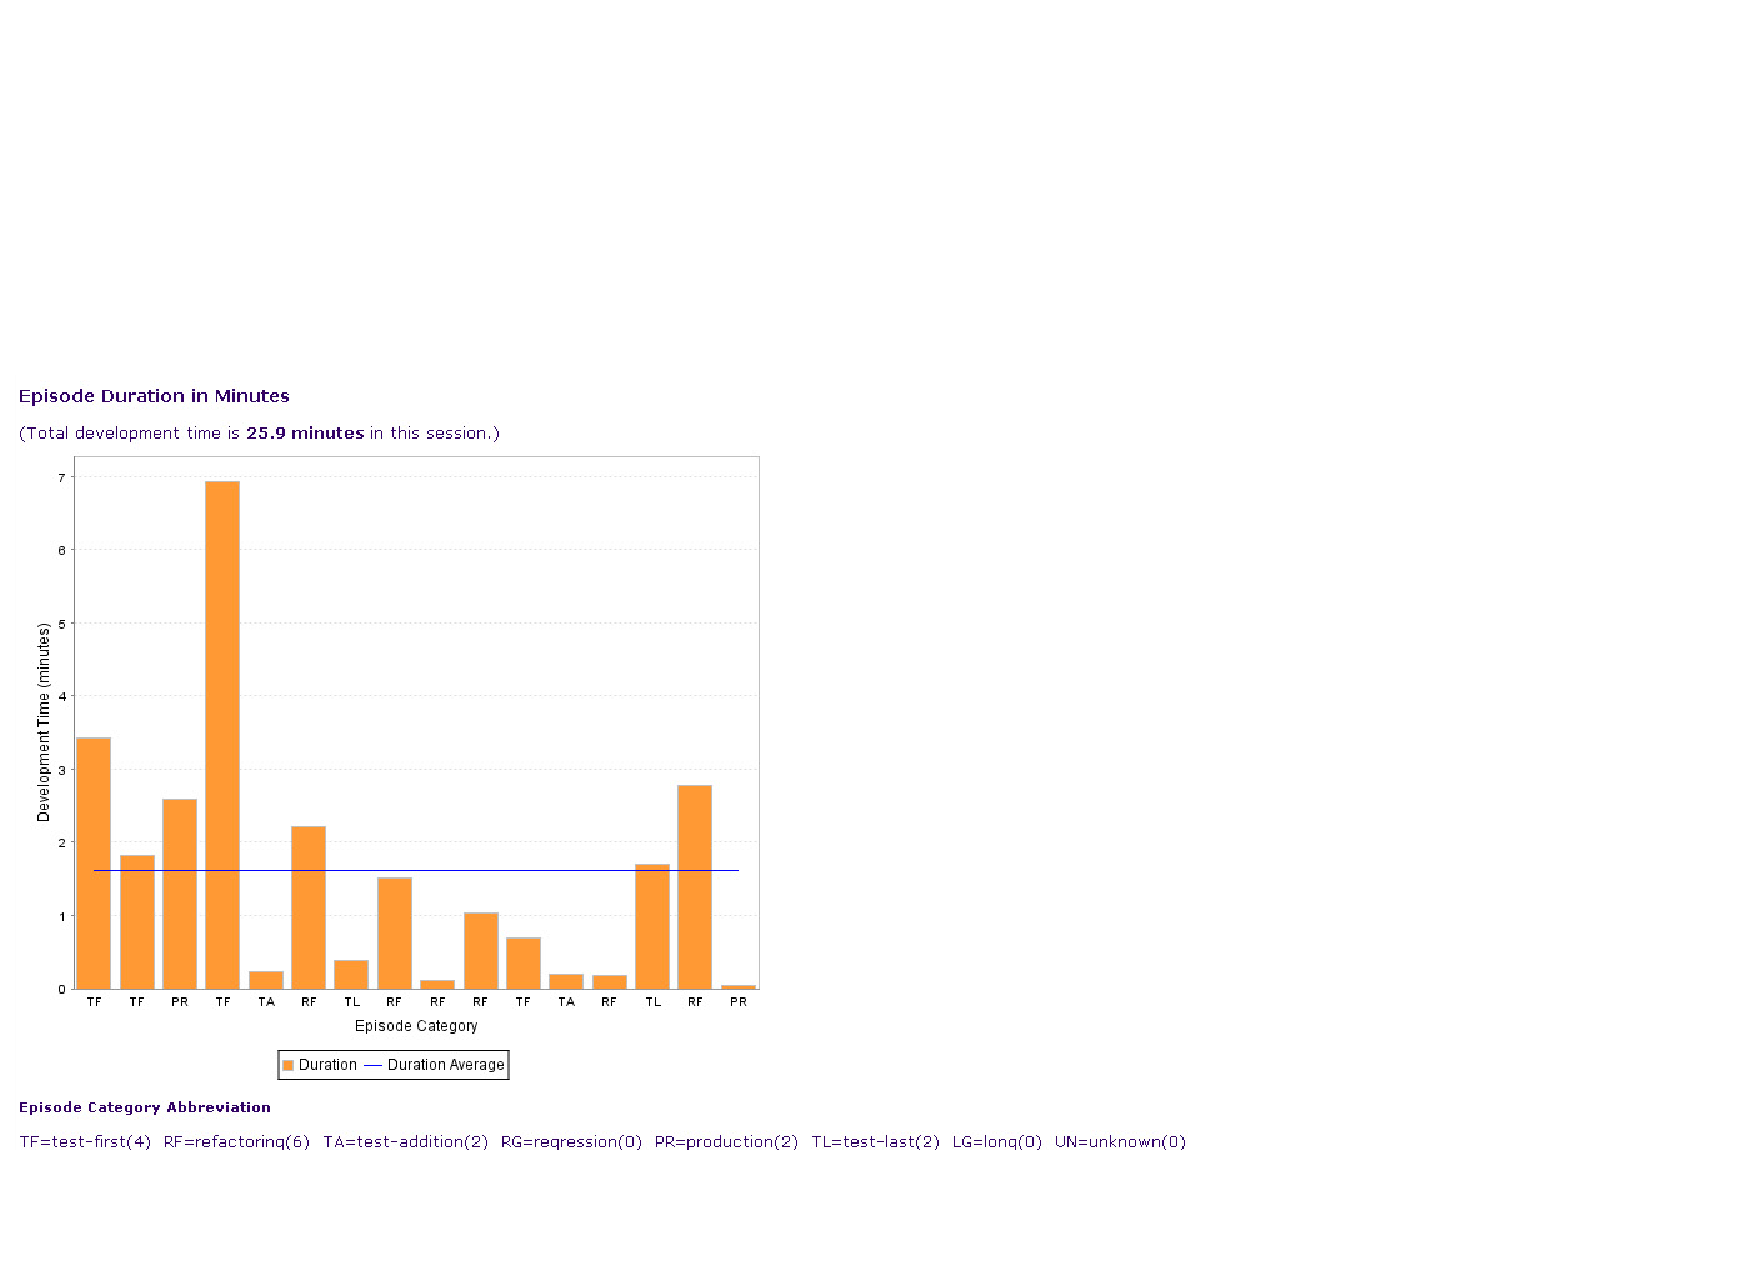
\includegraphics[width=0.7\textwidth]{figs/Zorro-Analysis-EpisodeDuration}
  \caption{Episode Duration}
  \label{fig:Zorro-Analysis-EpisodeDuration}
\end{figure}
The interpretation of this analysis is very straightforward. The 
horizontal axis has the two-letter acronym for each episode. 
The vertical axis is the episode duration in minutes. As we 
can see in Figure \ref{fig:Zorro-Analysis-EpisodeDuration},
with a little hill climbing at the beginning, tests were invoked 
frequently in this TDD programming session. 

Similarly, this analysis is applicable to any development methods 
where unit testing is practiced.  The durations in Figure 
\ref{fig:Zorro-Analysis-EpisodeDuration} are mostly short, which
supports the short duration claim made about TDD iterations. In 
practice, I rarely observed episodes that were longer than 30 minutes
in duration. In that case, the conformance to TDD is likely not 
stringent any more. A tabular report 
(Table \ref{tab:Zorro-Analysis-EpisodeDurationTable}) is also 
available for comparing episode duration differences among 
episode categories. 
\begin{table}[htbp]
\centering
  \caption{Duration Average by Episode Category}
  \begin{tabular}{|l|l|} \hline 
  Category  &   Average Duration (minutes) \\ \hline
  TF    & 3.2 \\ \hline
  RF    & 1.3 \\ \hline
  TA    & 0.2 \\ \hline
  RG    & 0   \\ \hline
  PR    & 1.3 \\ \hline
  TL    & 1  \\ \hline
  LG    & 0  \\ \hline
  UN    & 0 \\ \hline
  \end{tabular}
  \label{tab:Zorro-Analysis-EpisodeDurationTable}
\end{table}
 
\subsubsection{Episode Duration Bin}
The Episode Duration analysis lines up episodes with their 
durations, which is useful at displaying progressive changes. 
An alternative presentation is to arrange episodes with
close durations into a bin. Figure 
\ref{fig:Zorro-Analysis-EpisodeDurationBin} is an example
showing the Episode Duration Bin analysis. 
\begin{figure}[htbp]
  \centering
  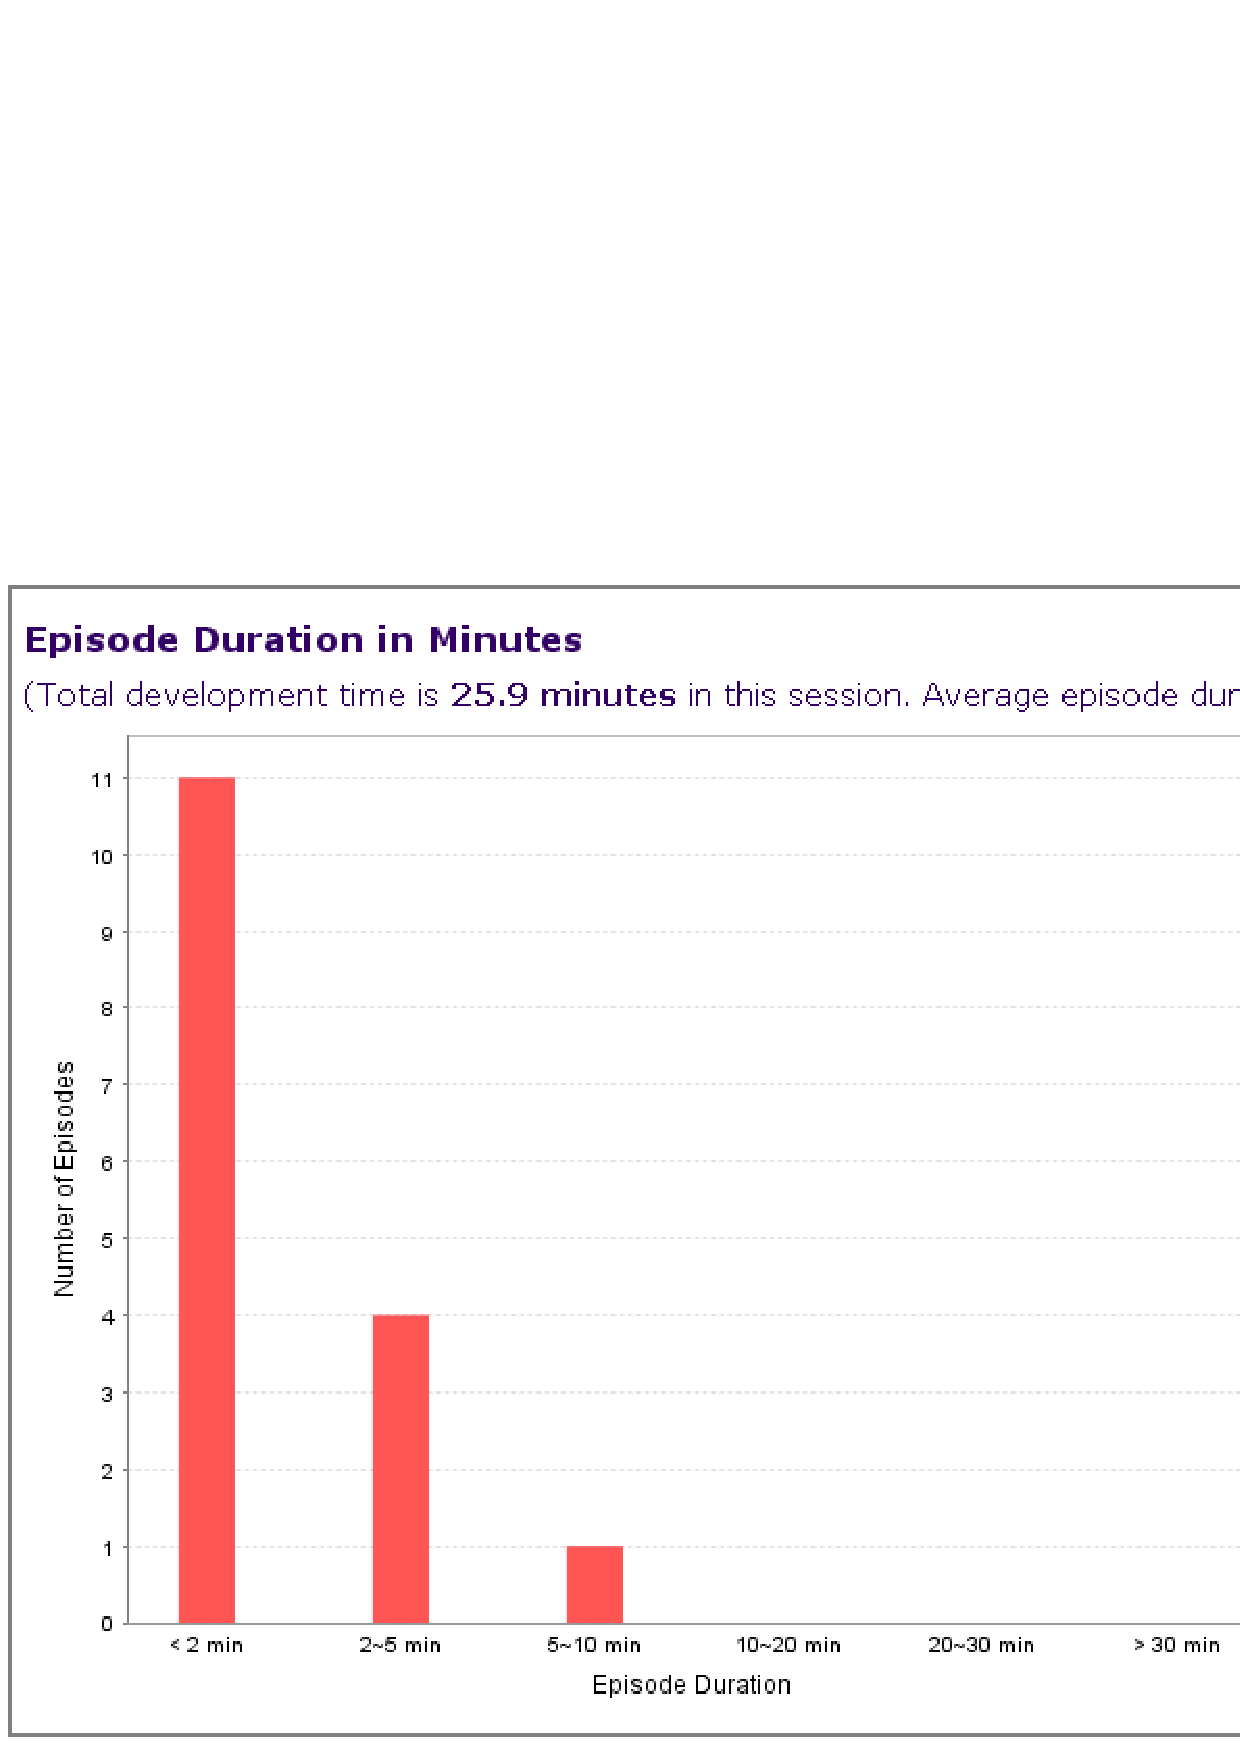
\includegraphics[width=0.7\textwidth]{figs/Zorro-Analysis-EpisodeDurationBin}
  \caption{Episode Duration Bin}
  \label{fig:Zorro-Analysis-EpisodeDurationBin}
\end{figure}
In Figure \ref{fig:Zorro-Analysis-EpisodeDurationBin}, the horizontal 
axis has a set of bins of episode durations, and the vertical axis 
is the number of episodes. 

Similar to the Episode Duration analysis, this analysis can be used to
verify TDD's short duration characteristic. An ideal TDD development 
session should have many short episodes with no or very few long episodes. 
If too many long episodes are observed, perhaps developers should take 
actions to develop and run tests more frequently. An episode duration 
distribution table (see Table \ref{tab:Zorro-Analysis-EpisodeDistribution})
is attached to this analysis.
\begin{table}[htbp]
\centering
  \caption{Episode Duration Distribution by Category}
  \begin{tabular}{llllllll} 
        Category & \textless 2 min & 2\~{}5 min & 5\~{}10 min & 10\~{}20 min & 20 \~{}30 min & \textgreater 30 min & Total \\ \hline
  TF      &  2  &  1 &   1  &  &        &  &  4  \\ 
  RF      &  4  &  2 &                  &  &    &  &    6  \\ 
  TA      &  2  &        &                      &  &    &  &    2  \\ 
  RG      &             &        &      &  &  &  &  0  \\ 
  PR      &  1  &  1 &                  &  &  &  &      2  \\ 
  TL      &  2  &        &                      &  &  &  &      2  \\ 
  LG      &     &        &                      &  &  &  &      0  \\ 
  UN      &             &        &                      &  &  &  &  0  \\ \hline
  Total &  11 &  4 &    1       & 0 & 0 & 0 &   16  \\  
  \end{tabular}
  \label{tab:Zorro-Analysis-EpisodeDistribution}
\end{table}

\newpage
\subsection{TDD Telemetry Streams}
\label{sec:Zorro-Analysis-Telemetry}
The analyses in Section \ref{sec:Zorro-Analysis} leverage
Zorro's recognition of TDD development behaviors. They can be used
to understand and improve TDD development for individuals. In order
to support project management and improvement, I implemented a
group of TDD telemetry streams in my research. Because Zorro 
abstracts software metrics into low-level development behaviors, 
the synergy of Zorro and Software telemetry allows better management 
of software projects developed in TDD. In this section, I will 
introduce Software telemetry, and present TDD telemetry analyses. 

\subsubsection{Software Project Telemetry and TDD Telemtry Reducers}
The Software project telemetry \cite{csdl2-04-11,csdl2-06-05} was 
developed by Qin Zhang in the Collaborative Software Development 
Lab at the University of Hawaii. It is an infrastructure to aggregate 
metrics data together to perform daily, weekly, or monthly analyses 
to support in-process software project management and decision makings. 
Software telemetry abstracts software metrics into streams, charts and 
reports. The telemetry stream contains a series of time-stamped events 
in the daily, weekly, or monthly granularity. The telemetry charts and 
reports provide visualization of telemetry streams. Detecting changes 
and covariance in the trend of telemetry streams enables an incremental, 
visible, and experimental approach to manage software 
projects \cite{csdl2-06-05}. 

The telemetry reducer is the extension point of Software telemetry, 
which can be used to extend the existing telemetry stream base.  
The following lists TDD telemetry reducers supplied in Zorro.
\begin{itemize}
\item \textbf{TDDPercent Reducer}:\\
Computes a single telemetry stream for percentage of TDD development 
time to overall development time. Alternatively, the percentage 
can also be the number of TDD compliant episodes to the number of 
total episodes. 

\item \textbf{TDDProductionDevTime Reducer}:  \\
Computes a single telemetry stream of development time on 
production code. Though its name suggests that this reducer 
is for TDD, it can actually be applied to other development 
methods as well.

\item \textbf{TDDTestDevTime Reducer}: \\
Computes a single telemetry stream of development time on
test code. Same as TDDProductionDevTime, it can be applied 
to development methods other than TDD if unit testing is 
used. 

\item \textbf{TDDDevTime Reducer}: \\
Computes a single telemetry stream of total development time. 
Note that Software telemetry already defines a DevTime, which
is different from TDDDevTime. The TDDDevTime can be 
thought as the summation of development time on production,
test, and others such as XML configuration files. 

\item \textbf{EpisodeAverageDuration Reducer}: \\
Computes a single telemetry stream of average episode duration.
It can be applied to TDD and other development methods. It 
indicates how frequently unit test is invoked. 

\item \textbf{TDDMemberProductionDevTime Reducer}: \\
Computes multiple telemetry streams for development time on
production code, one telemetry stream for each project member.

\item \textbf{TDDMemberTestDevTime Reducer}: \\
Computes multiple telemetry streams for development time on
test code, one telemetry stream for each project member.

\item \textbf{TDDMemberDevTime Reducer}: \\
Computes multiple telemetry streams for total development time, 
one telemetry stream for each project member.

\item \textbf{MemberEpisodeAverageDuration Reducer}: \\
Computes multiple telemetry streams for average episode durations, 
one telemetry stream for each project member.

\end{itemize}

\subsubsection{TDD Telemetry Analyses}
The availability of TDD telemetry reducers enables developers to 
invoke telemetry analyses using Zorro's recognized 
low-level development behaviors. 

Recall that a benefit of TDD is that the code developed in TDD
should be 100\% covered because no functional code is created
without a unit test (see Section \ref{sec:related-tdd}). So it 
would be interesting to study this claim. Since Zorro has the
TDDPercent Reducer, we can define a telemetry stream
reporting percentages of TDD development and correlate it with
the test coverage stream that is already included in Software
telemetry(Page 59 \cite{csdl2-06-05}). The following code
is a definition of the telemetry stream and chart for this
investigation.
\begin{verbatim}
  streams TDDPercent(type) = {
    "Percentage of Test-Driven Development", 
    TDDPercent(type) * 100
  };

  chart TDD-Coverage-Percentage-Chart() = {
    "Percentage of TDD Episodes (time) and Coverage", 
    (TDDPercent("time"), percentageYAxis("TDD \%")),
    (Coverage-Percentage("**", "line"), 
     percentageYAxis("Coverage \%"))
  };
\end{verbatim}

Figure \ref{fig:Zorro-Analysis-TDDPercentCoverage} 
is a weekly telemetry chart showing percentage of TDD development 
and test coverage.
\begin{figure}[htbp]
  \centering
  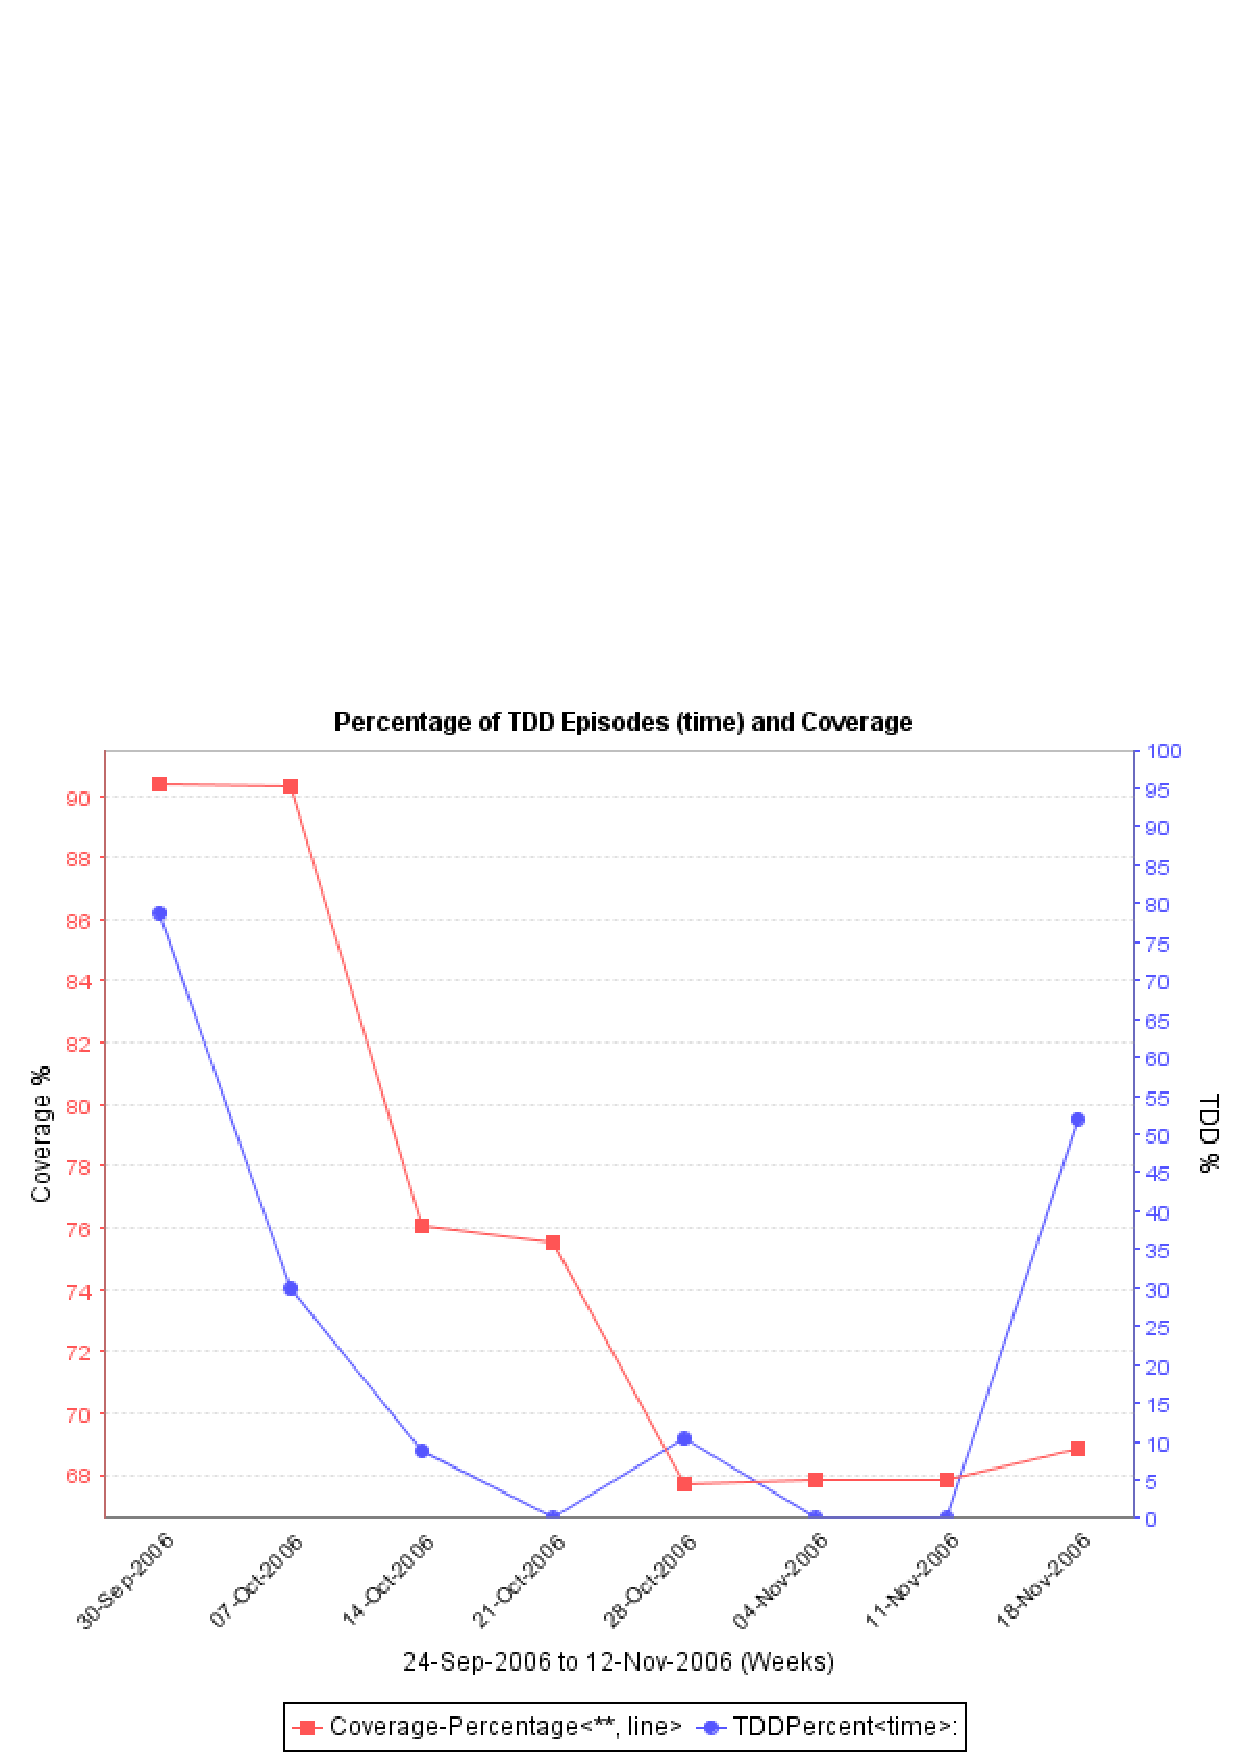
\includegraphics[width=0.8\textwidth]{figs/Zorro-TDD-Coverage}
  \caption{TDD Percentage and Testing Coverage}
  \label{fig:Zorro-Analysis-TDDPercentCoverage}
\end{figure}
From the week of Sep 30, 2006 to the week of Nov 18, 2006, I worked on the
Zorro software system and implemented Zorro's web validation interface.
Due to the fact that testing web interfaces requires a lot of additional
effort, my conformance to TDD dropped down significantly in that period. As
a result, the test coverage dropped from 90\% to below 70\% over the course
of eight weeks software development. Though we can not directly verify the
claim of 100\% test coverage characteristic of TDD, indeed the analysis
shows that deviating from TDD caused decrease of test coverage. In turn,
this indicates that TDD can help to improve test coverage.

\begin{comment}
The TDD telemetry reducers enable us to define telemetry streams
to monitor software project development.
\begin{figure}[htbp]
  \centering
  \includegraphics[width=0.8\textwidth]{figs/Zorro-Analysis-TDDPercent}
  \caption{Telemetry of TDD Percent}
  \label{fig:Zorro-Analysis-Telemetry-TDDPercent}
\end{figure}
\paragraph{Ratio of Effort on Test to Effort on Production}
\label{sec:RatioOfEffortOnTestToEffortOnProduction}

%% Tablelized chart. 
\paragraph{TDD Percentage vs. Testing Coverage}
\label{sec:TDDPercentageVsTestingCoverage}
\end{comment}

\section{Chapter Summary}
In this chapter, I introduced Zorro's implementation with the support 
of the Hackystat and SDSA frameworks. Zorro extends Hackystat's 
data collection, specializes SDSA's low-level development
behaviors inference for TDD, and supplies new functionalities to 
Hackystat. Zorro's development behaviors and conformance of TDD 
were detailed in this chapter, along with an introduction
to TDD analyses and telemetry reducers implemented in Zorro.
\chapter{Research Questions and Methodology}
\label{ch:Research}
The long-term goal of my research is to improve the consistency of empirical evaluation research on low-level software processes. As a step in this direction, I designed and developed the Software Development Stream Analysis (SDSA) framework (Chapter \ref{ch:Framework}) that can infer development behaviors using automatically collected in-process software metrics. I used the SDSA framework to specify a low-level software process called Test-Driven Development (TDD) and implemented Zorro, a software system that can recognize development behaviors and measure the developer's process conformance to TDD. If Zorro, a specification of the SDSA framework, can be experimentally validated, I will have provided evidence that SDSA is an enabling technique for recognizing at least certain types of low-level development activities. 

In order to validate Zorro, I designed a series of case studies including a pilot study,a classroom case study and an industrial case study. The purpose of the pilot and classroom validation studies was to validate Zorro's data collection and TDD behavioral inference 
in controlled environments. The purpose of the industrial case study was to explore how Zorro can be used by external researchers. Section \ref{sec:Research-Questions} introduces the central research questions of my thesis research. Section \ref{sec:Research-Methods} presents my research methods including participant observation, interview and survey. 

\section{Research Questions}
\label{sec:Research-Questions}

\begin{comment}
If Zorro can correctly recognize development behaviors of TDD, 
then it can be used to assess process conformance during daily 
practice of TDD, as well as during empirical evaluation of TDD
to improve construct validity (see Chapter \ref{ch:RelatedWork} 
for details). However, does Zorro infer developers' TDD development
behaviors correctly? Will it falsely categorize some non-TDD
development behaviors as TDD? Or, will it misinterpret some TDD
development behaviors as non-TDD? To answer these questions, we 
need to conduct Zorro validation studies. 
\end{comment}

The central research questions of the Zorro validation studies were:
\begin{itemize}
\item Q1: Can Zorro automate the recognition of TDD behaviors
using automatically collected software metrics?  

This question can be further divided into three sub-questions:
   \begin{itemize}
     \item Can Zorro collect software metrics correctly?
     \item Does Zorro collect the necessary software metrics?
     \item Can Zorro infer TDD behaviors correctly based upon 
     automatically collected software metrics?
   \end{itemize}

\item Q2: How useful is Zorro? 

This question is hard to answer but it can be divided into three sub-questions based upon users' roles.

\begin{itemize}
\item For beginners, can Zorro help them improve their compliance to TDD?
\item For experienced TDD practitioners, will Zorro help them improve their TDD practice by providing them with new insight into their TDD development behaviors?
\item For researchers, can Zorro help them reach legitimate research conclusions on TDD experiments by providing them with TDD process conformance information?
\end{itemize}

\end{itemize}

\section{Research Methodology}
\label{sec:Research-Methods}

Answering the above research questions requires a ``mixed methods'' research methodology according to \cite{Creswell:03}. Question Q1 can be investigated using the participant observation. In order to investigate the research question Q2, we need to collect users' feedback or interview them. 

To use the participant observation method, we can observe participants in the field, take notes about their development activities and behaviors to provide an independent data source for validating Zorro's data collection and TDD behaviors inference. However, this manual participant observation method \cite{Creswell:03} does not work for studying low-level software development activities that could occur in seconds and minutes. It is simply too demanding for the observer to record all of the necessary information about a low level software process, where significant events can occur every few seconds. Thus, I developed a recording tool called ``Eclipse Screen Recorder'' (ESR) to assist participant observation. ESR is an Eclipse plugin that can generate a QuickTime movie containing time-stamped screen shots of the Eclipse window at regular intervals. With ESR, observers will not need to worry about missing rapid development activities. 

Figure \ref{fig:ESR} illustrates the Eclipse window with ESR installed. The two pictured buttons on the toolbar menu are defined by ESR. Pressing the green button can start the recording process and make the red button become enabled. The recorder will stop if either the red button is pressed or Eclipse is closed. 
\begin{figure}[htbp]
  \centering
  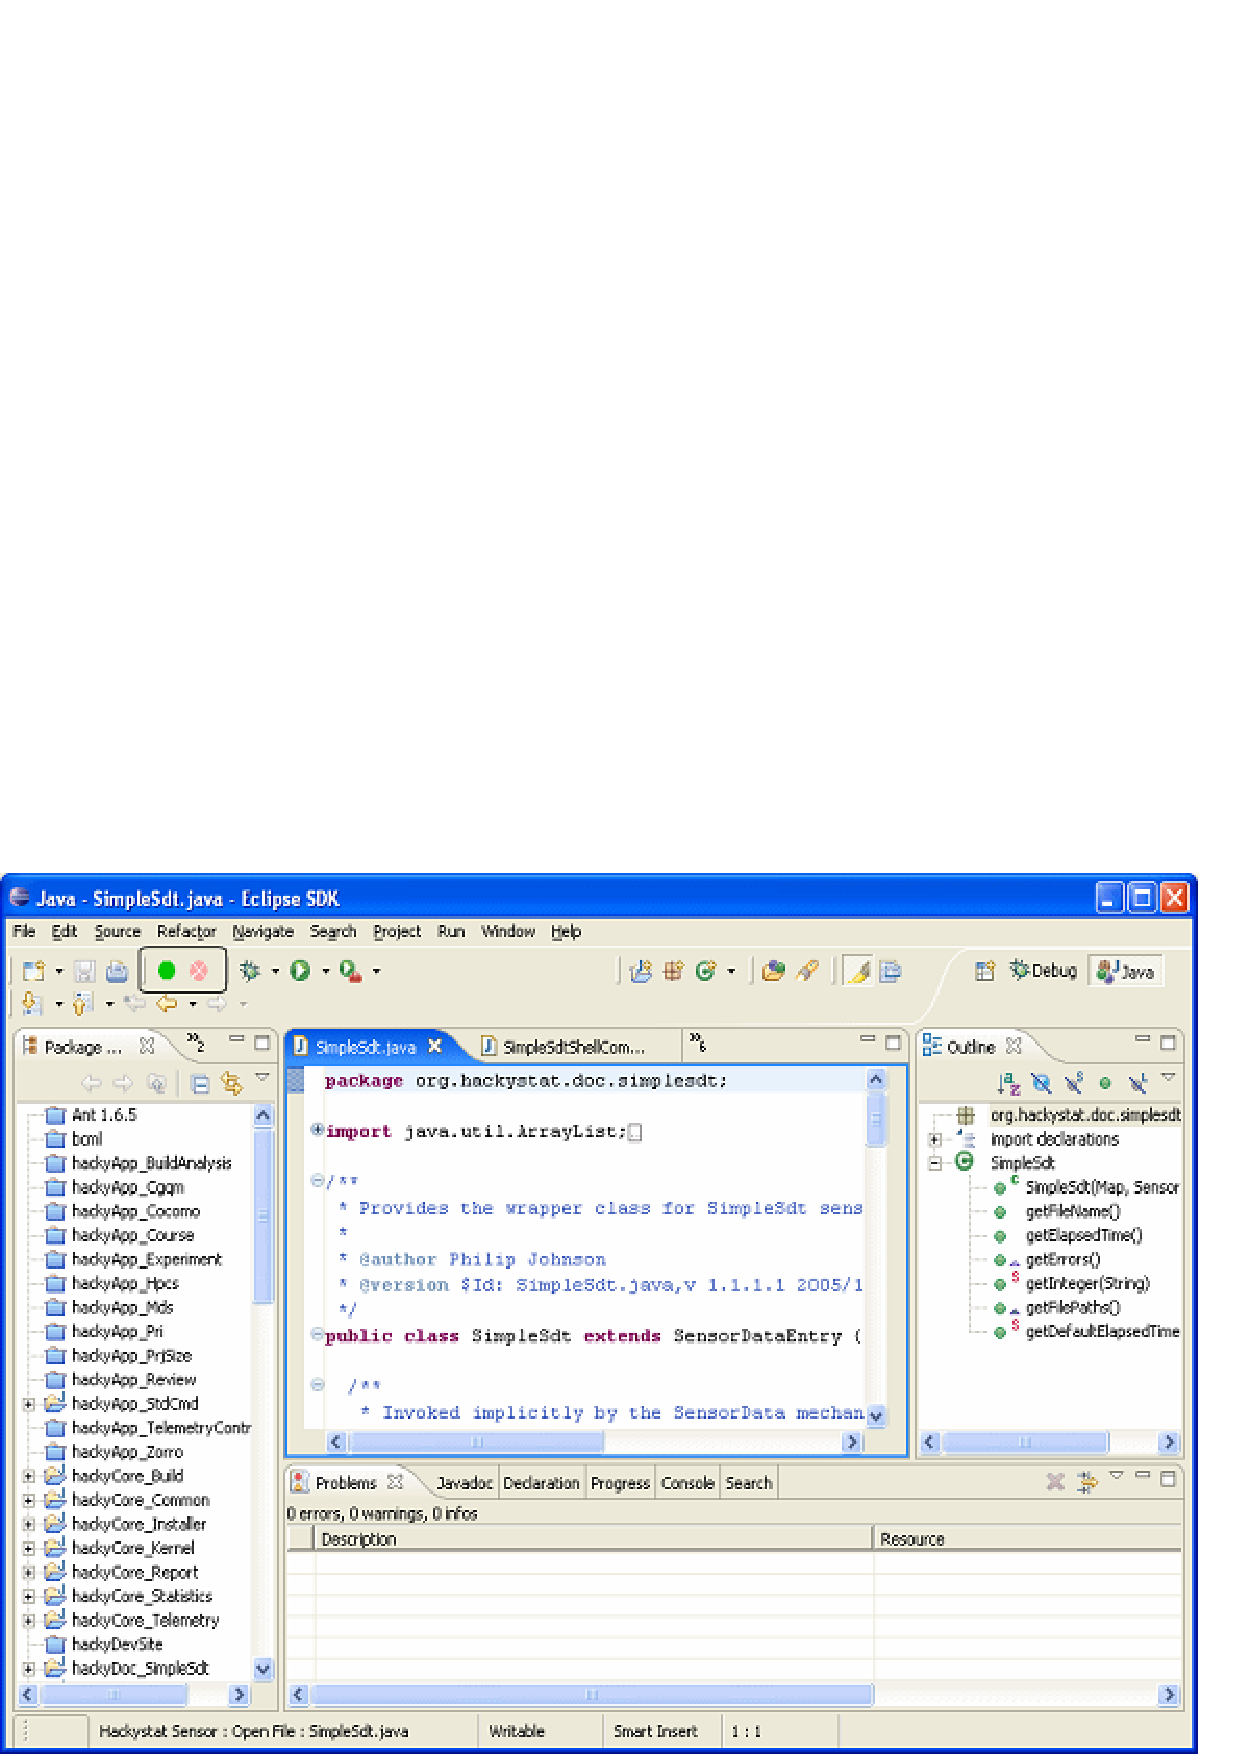
\includegraphics[width=0.8\textwidth]{figs/ESR}
  \caption{Eclipse Screen Recorder}
  \label{fig:ESR}
\end{figure}
Figure \ref{fig:ESR-Video} in Chapter \ref{ch:Introduction} illustrates the recorded movie being played by QuickTime. The embedded timeline at bottom of videos (See Figure \ref{fig:ESR-Video}) can be used to synchronize videos with development activities collected by Zorro for validation. ESR allows customization of recording rate (0.5-2 frames per second), picture quality, and resolution. One frame/second was found to be sufficient for validation, generating file sizes of approximately 7-8MB per hour of video. 

The development of Zorro was iterative and incremental. So was the validation of Zorro. I have conducted three case studies --- a pilot study, a classroom case study, and an industrial case study. Next, I will introduce the research methods I used in these case studies.

\subsection{Pilot Study}

I designed and implemented the Zorro software system based upon descriptions in books \cite{Beck:03,Astels:03,Newkirk:04,Link:03,Hunt:03} and my observation of TDD in practice. By Spring 2005, I had enhanced the Hackystat Eclipse sensor to collect necessary development activities, designed the SDSA  framework and implemented the Zorro software system to infer TDD development behaviors automatically. In the following Fall semester, I conducted a pilot Zorro validation case study.

The purpose of the pilot study was to test ESR as a tool to provide independent evidence for validating Zorro, as well as to validate Zorro's data collection and TDD behavior inference. The research method was participant observation using ESR as the data collection tool. I played recorded QuickTime videos to observe participants' TDD development activities and behaviors for Zorro validation. 

\begin{comment}
The specific research questions for the pilot study were:
\begin{itemize}
 \item Q1a: Does Zorro collect enough low-level development 
 activities to infer TDD behaviors?
 \item Q1b: Does Zorro's inference of TDD agree with analyses 
 based upon participant observation?
 \item Q1c: Is ESR a suitable tool for Zorro validation study?
\end{itemize}
\end{comment}


\subsection{Classroom Case Study}
The pilot study showed that participant observation with ESR is a suitable research method for conducting Zorro validation study. Though Zorro was not perfect at collecting necessary software metrics and inferring TDD behaviors, the pilot demonstrated that it was promising. Based on research results from the pilot study, I improved Zorro's data collection, enhanced Zorro's TDD behaviors inference, added heuristics on process conformance of TDD, and provided many TDD analyses and telemetry reducers (See Chapter \ref{ch:Zorro}). With these improvements, I conducted an extended validation study on Zorro in the software engineering classes at the University of Hawaii in Fall 2006. 

\begin{comment}
I addressed both of the research questions Q1 and Q2. The specific 
research questions for this study were:
\begin{itemize}
\item{Q2a: Does Zorro collect sufficient software development 
activities for episode partitioning and TDD behavior inference?}
\item{Q2b: Does Zorro's inference of TDD behaviors agree with
analyses based upon participant observation?}
\item{Q2c: Does Zorro's inference of TDD behaviors agree with what
participants believe to be their TDD behaviors?}
\item{Q2d: Does Zorro provide useful information for beginners to
understand TDD and improve their TDD development?}
\end{itemize}
\end{comment}

The purpose of the classroom case study was to validate Zorro in a controlled environment and investigate its usefulness for TDD beginners. The research method of the validation was also participant observation. Participants developed software using TDD in Eclipse with instrumentation including the Hackystat Eclipse sensor and ESR. ESR served as the data collection tool for participant observation and the recorded videos were analyzed to validate Zorro.

A caveat with the pilot study was that I, the author of the Zorro software system, analyzed the recorded videos for Zorro validation. This creates a ``construct validity'' threat with regard to this experiment design because ESR was the only source of evidence and my analysis could be biased. Therefore, in order to increase the construct validity of classroom case study, multiple sources of evidence were used according to suggestions from Yin in \cite{Yin:03} (Page 34). Participants' comments were the third source of information I used to cross-validate video analysis results. Prior to the study, I developed a Zorro validation wizard in web pages to let participants comment. 

To explore whether Zorro can help TDD beginners, I interviewed participants on their TDD development experiences. After the interview, each participant used the Zorro validation wizard to analyze his/her TDD development behaviors. Meanwhile, an embedded survey was conducted to evaluate Zorro's usefulness. To improve quality of the survey, I asked participants to justify their answers verbally. 

%to address the research question Q2d.

\subsection{Industry Case Study}
In Spring 2007, I conducted an industry case study to test Zorro's usefulness to TDD researchers. Using Zorro as a tool to assess TDD process conformance, Dr. Geir Hanssen and Dr. Tor Erlend F{\ae}gri from SINTEF ICT of Norway conducted a TDD vs. non-TDD comparison study in a Norwegian software company.

\begin{comment}
I focused on the research question Q2 to evaluate Zorro's usefulness
in this study. The specific questions were:
\begin{itemize}
\item Question Q3a: Can Zorro be deployed? 
\item Question Q3b: Does Zorro infer the TDD behaviors correctly as
participants' perception?
\item Question Q3c: Are Zorro's TDD analyses useful for participants?
\item Question Q3d: How can Zorro be used to assist TDD research?
\end{itemize}
\end{comment}

The purpose of this study was to explore how Zorro can be used by researchers to increase quality of TDD's evaluation research. I deployed Zorro in the software company, assisted the project manager and the researcher on analyzing process conformance data, and conducted a survey at the end of the study. 

% to address research questions Q3a-Q3d. 

\section{Chapter Summary}
This chapter introduced my research statement and Zorro's validation case studies. The central research questions were: (1) Can Zorro automate the recognition of TDD behaviors using automatically collected software metrics? and (2) How useful Zorro is?  To address these questions, I have conducted a pilot study, a classroom case study and an industry case study in which I used research methods such as participant observation, interviews and surveys. In order to improve the quality of data collection for participant observation, I developed ESR, a tool that can record the Eclipse window in high fidelity. Both the pilot study and the classroom case study used ESR as a data collection tool for Zorro validation. 

\begin{comment}

In Zorro, I converted the knowledge of TDD practice into a set of
rules to classify development behaviors of TDD on the development
stream consisting of automatically collected software metrics. 
So the software metrics that are related to TDD development 
behaviors must be collected, and the TDD inference rules must be 
correct. 

Thus, in order to validate Zorro, we need an independent
source that can oversee the low-level development activities of
TDD and 

a third party tool that can oversee the data collection process
and examine the inferred results. 


Beck literally introduced the 
development method of TDD in \cite{Beck:03}, which is the main resource
I used for 

Whether Zorro can automate the recognition of development behaviors of 
TDD relies on the capability of software metrics collection, as well as 
the correctness of inference rules. Thus, in order to validate Zorro,
we need an independent source of information of development activities
to compare to Zorro's. 

As a result, we can study process 
conformance using SDSA to improve the consistency of empirical 
research on low-level software processes. 

The long-term goal of my research is to understand how to characterize
and improve low-level software development behaviors.  As a step in
that direction, I am focusing for my Ph.D. research on a specific kind
of low-level software development behavior: Test-Driven
Development. The Zorro system, which attempts to infer TDD low-level
development behaviors, provides a way to partially evaluate the
overall approach and begin to understand its strengths and
limitations.

Zorro infers developer's TDD development behaviors using SDSA. It is
easy for software developers to collect in-process development
activities using Hackystat sensors, and it is also easy for them to
evaluate their TDD development behaviors using Zorro. If Zorro's TDD
inference is correct, then we can use it to assess TDD process
conformance during the daily practice of TDD as well as during empirical
studies of TDD. However, does Zorro infer developers' TDD development
behaviors correctly? Will it falsely categorize some non-TDD
development behaviors as TDD? Or, will it misinterpret some TDD
development behaviors as non-TDD? To answer these questions, we need 
to conduct validation studies of Zorro. Some of the most important research
questions are: 
\begin{itemize}
\item Q1: Can Zorro automate the recognition of Test-Driven Development
using automatically collected low-level software development activities?  
\item Q2: Can Zorro help to improve the practice of TDD? 

This is a hard question, but we can divide it into three small questions
with regard to user's roles.
   \begin{itemize}
   \item For beginners, can Zorro help them improve the compliance to TDD?
   \item For experienced TDD practitioners, will Zorro help them
   improve their TDD practice by analyzing their TDD development
   behaviors?
   \item For researchers, can Zorro help them reach legitimate
   research conclusions on TDD experiments by providing the TDD
   process conformance information.
   \end{itemize}
\end{itemize}

Answering these questions requires a ``mixed methods'' research strategy
\cite{Creswell:03}. Questions Q1 can be investigated by evaluating 
Zorro's data collection and TDD inference capability using field observation
research method. Investigating question Q2 requires research methods such  
as collecting users' feedback or interviewing them. In my research, 
I designed a series of case studies using these research methods to 
investigate the research questions I presented above.

\section{Evaluation Methods}
\label{sec:EvaluationMethods}
This chapter introduces three Zorro validation studies: a pilot study,
a case study with students from the software engineering class as
participants, and an external collaborative case study with the TDD
community of developers and researchers. Zorro uses low-level software
development activity data to infer developer's TDD behaviors.  In
order to validate its capabilities of data collection and TDD behavior
inference, a secondary data source must be used. In my dissertation
research, I will introduce two ways to provide the secondary data:
recording individual developer's TDD development process using the
Eclipse Screen Recorder (ESR) \cite{esr}; and gathering developer's
feedback to their TDD behavior inference results using the Zorro
validation wizard.  I have already used the ESR approach in the pilot
study. In the second case study, I will plan to use both approaches.

\end{comment}
\chapter{Pilot Study}
\label{ch:Pilot}

I employed the case study research strategy \cite{Yin:03} to empirically study Zorro's TDD development behaviors inference. In order to validate Zorro, I conducted a pilot study at the University of Hawaii in Fall 2005. This study shows that the participant observation research method using ESR is an acceptable research method for Zorro validation and it also shows that Zorro can accurately recognize development behaviors of TDD in a simple project development setting.

\section{Purpose of the Study}
The pilot study served as a dry-run test to the chosen case study research strategy. As mentioned in Chapter \ref{ch:Research}, the purpose of the pilot study was to test ESR, as well as to validate Zorro's data collection and behaviors inference of TDD.

\section{Research Questions}
\label{sec:Pilot-Questions}

The specific research questions for the pilot study were:
\begin{itemize}
 \item Q1a: Is ESR a suitable tool for Zorro validation study?
 \item Q1b: Does Zorro collect enough low-level development activities to
   infer developer's TDD behaviors?
 \item Q1c: Does Zorro's inference of TDD agree with analyses based upon
   participant observation?
\end{itemize}

Note that these specific research questions corresponded to the main research questions Q1: \textit{Can Zorro automate the recognition of TDD behaviors using automatically collected software metrics?}

\section{Experiment Design}
\label{sec:Pilot-Design}
The pilot study was largely a one-shot case study in which participants were exposed to TDD. Creswell \cite{Creswell:03} suggests the following notation for it:
  \begin{tabular}{p{0.5cm}lp{1cm}l} 
    & Group A  & & X ------ O
  \end{tabular}

where group A represents a group of participants, X represents an exposure of a group to an experimental variable or event, and O represents an observation or measurement on an instrument. In this study, TDD was the treatment and Zorro was the instrument.  

\subsection{Participants}

In this study, I recruited seven experienced Java developers who were 
familiar with unit testing. 

\subsection{Materials}
The programming problem was the stack data structure. I gave the developers user stories which described the activities they were to perform in order to implement the stack.. Eclipse was the development tool. In addition, I also provided Doshi's TDD Rhythm \cite{TDDRhythm} and TDD Quick Reference Guide \cite{TDDQuickReference} as supporting materials. In order to improve participants' commitment to TDD, a To-Do list was supplied as the reference. 

\subsection{Instrument}
I instrumented participants' TDD development processes with the Hackystat Eclipse sensor and ESR. Participants were required to install the Hackystat Eclipse sensor and send the collected development activities to a remote Hackystat server. They also installed ESR which recorded their Eclipse windows as they participated in this study. 

\subsection{Procedure}
Since the pilot study configuration was very simple, participants were given the option to either work on a lab computer or on their own computers at home. For those who opted to work at home, I provided detailed step-by-step instructions to them.  

\begin{enumerate}
\item{Setup} 

Prior to the study I confirmed that the lab computer had the following software installed: 
  \begin{itemize}
    \item JDK 
    \item Eclipse IDE 
    \item Hackystat Eclipse Sensor \cite{HackystatSensorInstallation:06}
    \item Eclipse Screen Recorder \cite{esr}
  \end{itemize}
When participants chose to work at home on their own computers, I asked them to configure these software before participating in this study.

\item{Introduction to TDD}

When participants did not have prior knowledge of TDD, I briefly introduced TDD to them using Beck's simple abstraction of TDD: Red/Green/Refactor. 

\item{Development in TDD} 

Stack is a well-known data structure that works according to the Last-In-First-Out (LIFO) principle. The participants developed a program to implement the Stack data structure using TDD. I provided  them with three documents: the graphic illustration of TDD rhythm, the TDD reference guide, and the user stories of stack with a To-Do list. They are available at Appendix \ref{app:PilotStudyMaterial}. In this step, both the Hackystat Eclipse sensor and ESR were turned on.

\item{Data Collection}

The Hackystat Eclipse sensor collected and sent development activities to a remote Hackystat server. I asked participants' permissions to access their data for this study. For videos recorded by ESR, I asked participants to send them to me via email attachments. 

\end{enumerate}

\section{Threats to Validity}
There were several threats to construct validity. One of them was that some participants did not know TDD prior to the study. For these participants, I gave them a brief tutorial at the beginning of the study, and provided a graphic illustration of the rhythm \cite{TDDRhythm} and the reference guide \cite{TDDQuickReference} of TDD. Another threat was the process conformance of TDD. To minimize its effects, I used Stack, a simple and well-known data structure, and provided user stories with a To-Do list to help participants comply with TDD.  

With regard to validity of data collection, I used unobtrusive data collection utilities: Hackystat Eclipse Sensor and ESR. Both tools required a little overhead from participants \cite{csdl2-03-12,Hackystat} at the beginning and at the end of the study.

There were two external validity threats in this study. The first one was the simplicity and stringency of TDD. In the pilot study, I interpreted TDD as strictly as Beck suggested in \cite{Beck:01,Beck:03} and Doshi recommended in \cite{TDDRhythm,TDDQuickReference}. The second one was that only 7 developers participated in this study. To address both of them, I conducted an extended validation study and an industrial case study in my thesis research following this pilot study.

\section{Data Analyses}
\label{sec:Pilot-Analysis}
I collected two sources of data about TDD development in this study. The Hackystat Eclipse sensor collected low-level development activities that were used by Zorro to recognize participants' TDD development behaviors. The development process videos recorded by ESR were the second source of data that served as participant observation. I used the observational results from videos recorded by ESR to validate Zorro in data analyses.

\subsection{Infer Development Behaviors with Zorro}
To use Zorro, I defined a Hackystat project for each participant and then conducted the ``TDD Development Stream'' analysis provided by Zorro. Figure \ref{fig:gui} illustrates the inferred results using my own data. 
\begin{figure}[htbp]
  \centering
  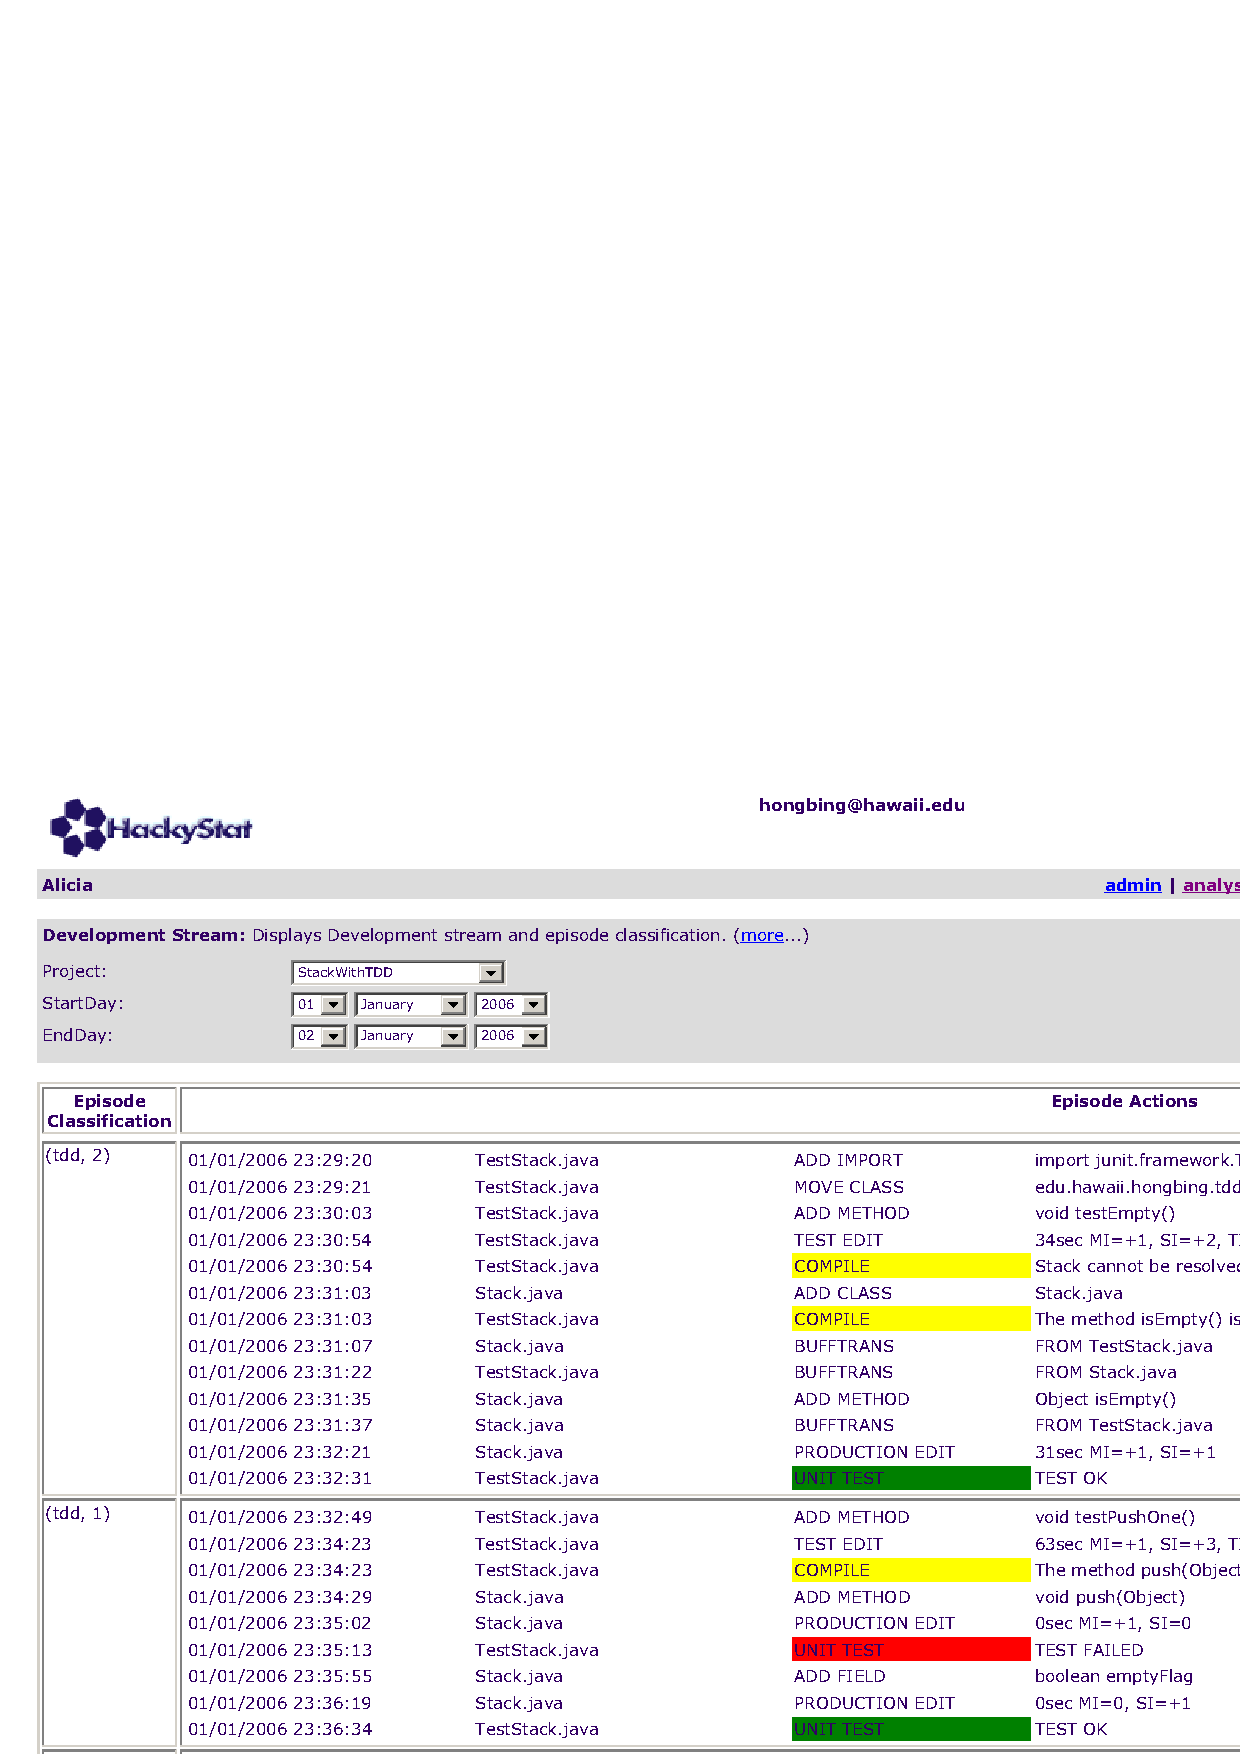
\includegraphics[width=1.0\textwidth]{figs/Zorro-Gui}
  \caption{TDD Development Stream Analysis}\label{fig:gui}
\end{figure}
Recall that Zorro partitions development streams using the ``Test-Pass'' tokenizer as described in Chapter \ref{ch:Zorro}, which yielded a sequence of ``Test-Pass'' episodes as shown in Figure \ref{fig:gui}. The ``Episode Actions'' column on the right displays episodes' internal structures. Corresponding to the Red/Green/Refactor metaphor of TDD, Zorro highlights test failures in red and test passes in green backgrounds. In addition, compilation errors were highlighted in a yellow background. The ``Episode Classification'' column on the right presents development behaviors inferred by Zorro. 

The inferred results were summarized in Table \ref{tab:ZorroPilotStudy}. For each participant, it lists the development duration and number of total, TDD, Refactoring, Test-Last and Unclassified episodes.
\begin{table}[htbp]
\centering
  \caption{Zorro's Inference Results for Pilot Study}
  \begin{tabular}{|r|r|r|r|r|r|r|}
  \hline
    Subject ID & Duration & Episode & TDD & Refactoring & Test-Last & Unclassified \\ \hline
    1 & 44:53 & 15 &  6 &  1 &  7 & 1 \\ \hline
    2 & 28:17 & 13 &  5 &  0 &  8 & 0 \\ \hline
    3 & 48:00 & 14 &  9 &  0 &  5 & 0 \\ \hline
    4 & 66:32 & 14 &  5 &  1 &  8 & 0 \\ \hline
    5 & 43:14 & 16 &  3 &  1 &  7 & 5 \\ \hline
    6 & 45:57 & 11 &  4 &  0 &  7 & 0 \\ \hline
    7 & 32:40 &  9 &  4 &  1 &  3 & 0 \\ \hline \hline
    Total &   & 92 & 36 &  4 & 45 & 6 \\ 
  \hline
  \end{tabular}
  \label{tab:ZorroPilotStudy}  
\end{table}
According to Table \ref{tab:ZorroPilotStudy}, participants spent 28-45 minutes to implement Stack using TDD and yielded 92 episodes. Zorro recognized 86 of them, which accounts for 93.6\% of all episodes. Interestingly, among 6 unrecognizable episodes, 5 of them were from one participant only. It was also notable that participants almost never refactored, and they did ``Test-Last'' half of the time (in the unit of episode number). Here ``Test-Last'' means that participants write test code after production code has been implemented, which is the opposite side of TDD.

In the pilot study Zorro inferred TDD behaviors as ``TDD'', ``Refactoring'' or ``Test-Last''. This development behaviors classification reflected Beck's \cite{Beck:03} simple abstraction of TDD. Further research found that this classification can not represent actual TDD developments, and thus a more sophisticated TDD development behaviors classification schema was developed as described in Chapter \ref{ch:Zorro}.

\subsection{Participant Observation}
\label{sec:Pilot-Observation}
An ESR video contains time-stamped Eclipse windows that were captured at the rate of one frame per second. I played and watched the recorded videos as a form of participant observation. Figure \ref{fig:EsrVideo} is a screen-shot showing an ESR video that I played using QuickTime\cite{QuickTime}.
\begin{figure}[htbp]
  \centering
  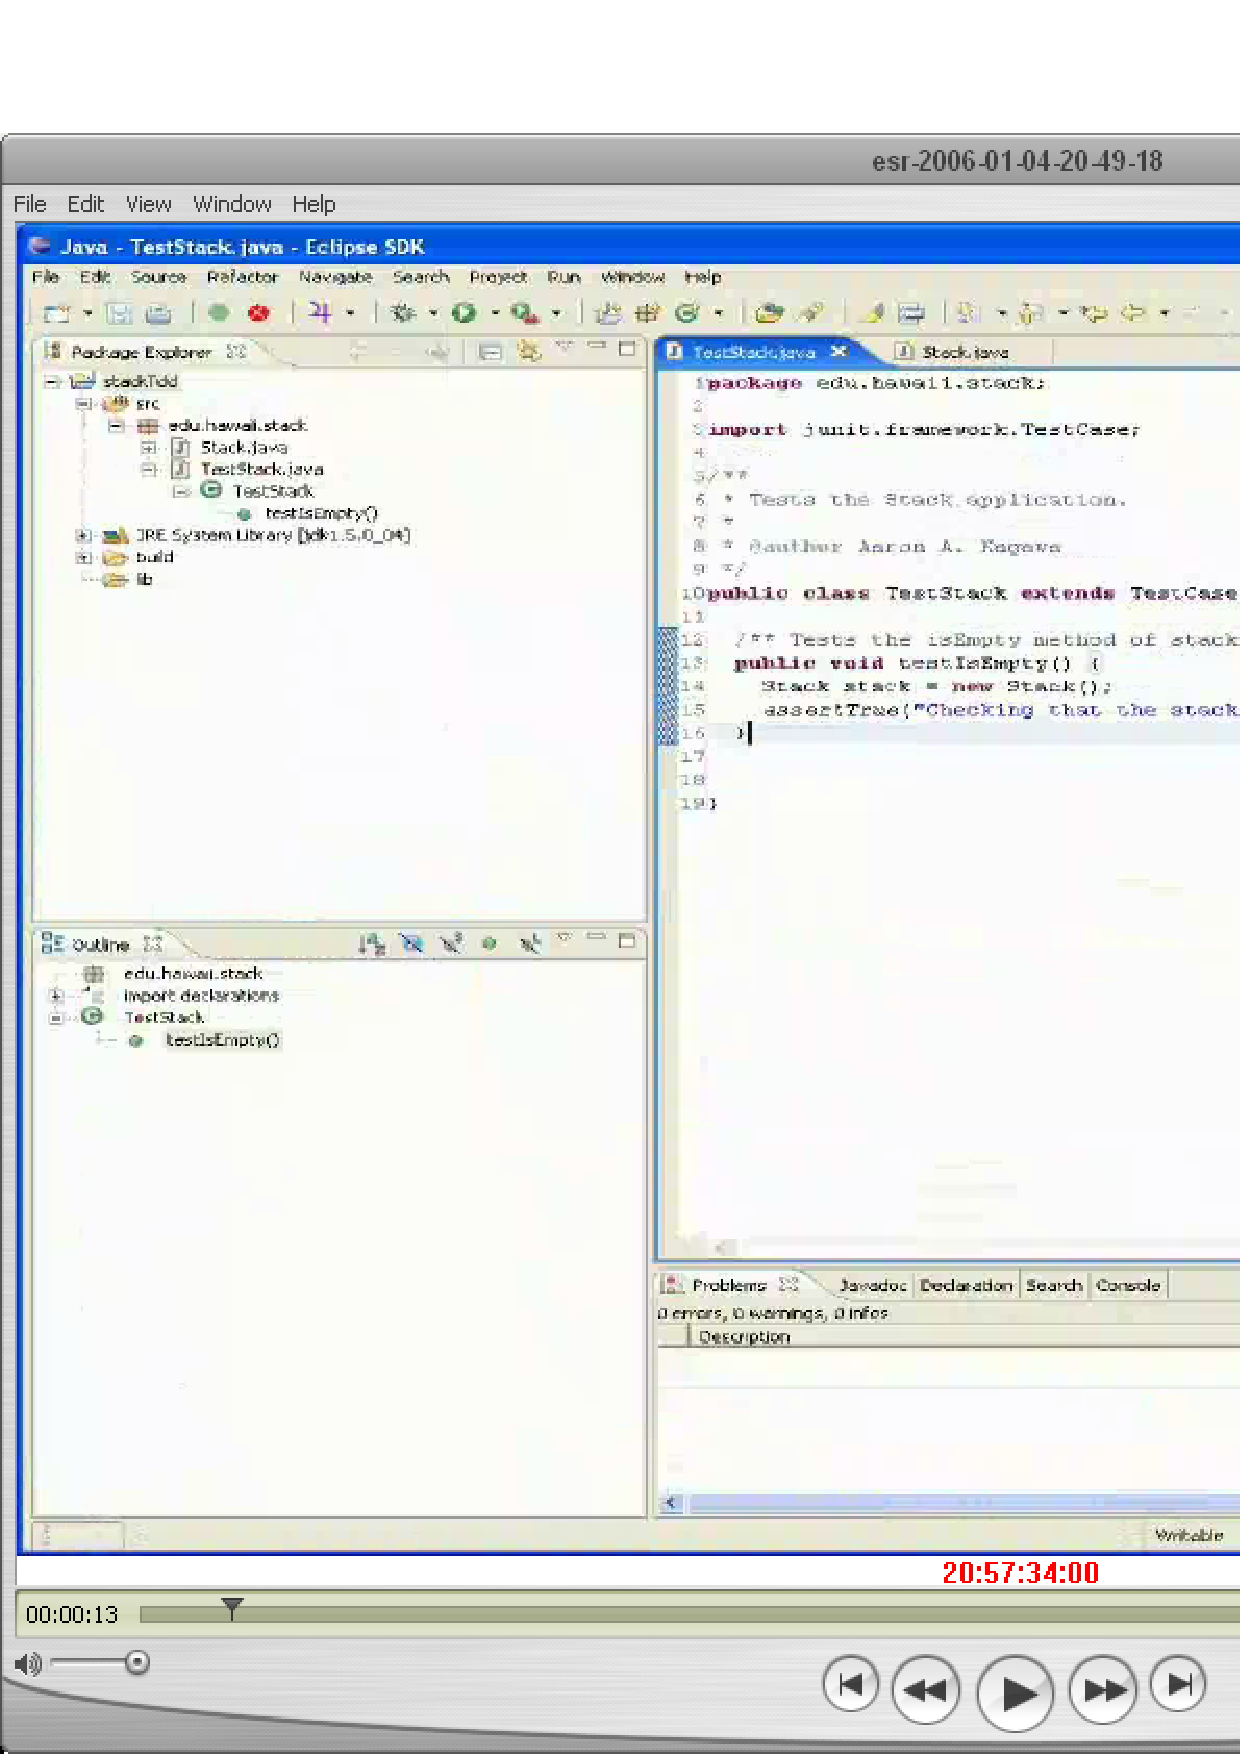
\includegraphics[width=0.9\textwidth]{figs/ESR-Video}
  \caption{ESR Video}
  \label{fig:EsrVideo}
\end{figure}
At the time when Figure \ref{fig:EsrVideo} was captured, the participant who produced the video had just finished a TDD iteration ending with a successful unit test invocation. The video also includes a time-line at the bottom indicating the time when the window was captured. Note that the comment at the top-right corner in Figure \ref{fig:EsrVideo} was not part of the video. I added this remark in my observation analysis. 

When I observed a TDD-realted activity in the ESR videos, I recorded it into an Excel spreadsheet for bookkeeping (See Figure \ref{fig:VideoExcelScript}). Each activity has a start time, an end 
time, an abstract, and additional annotations.
\begin{figure}[htbp]
  \centering
  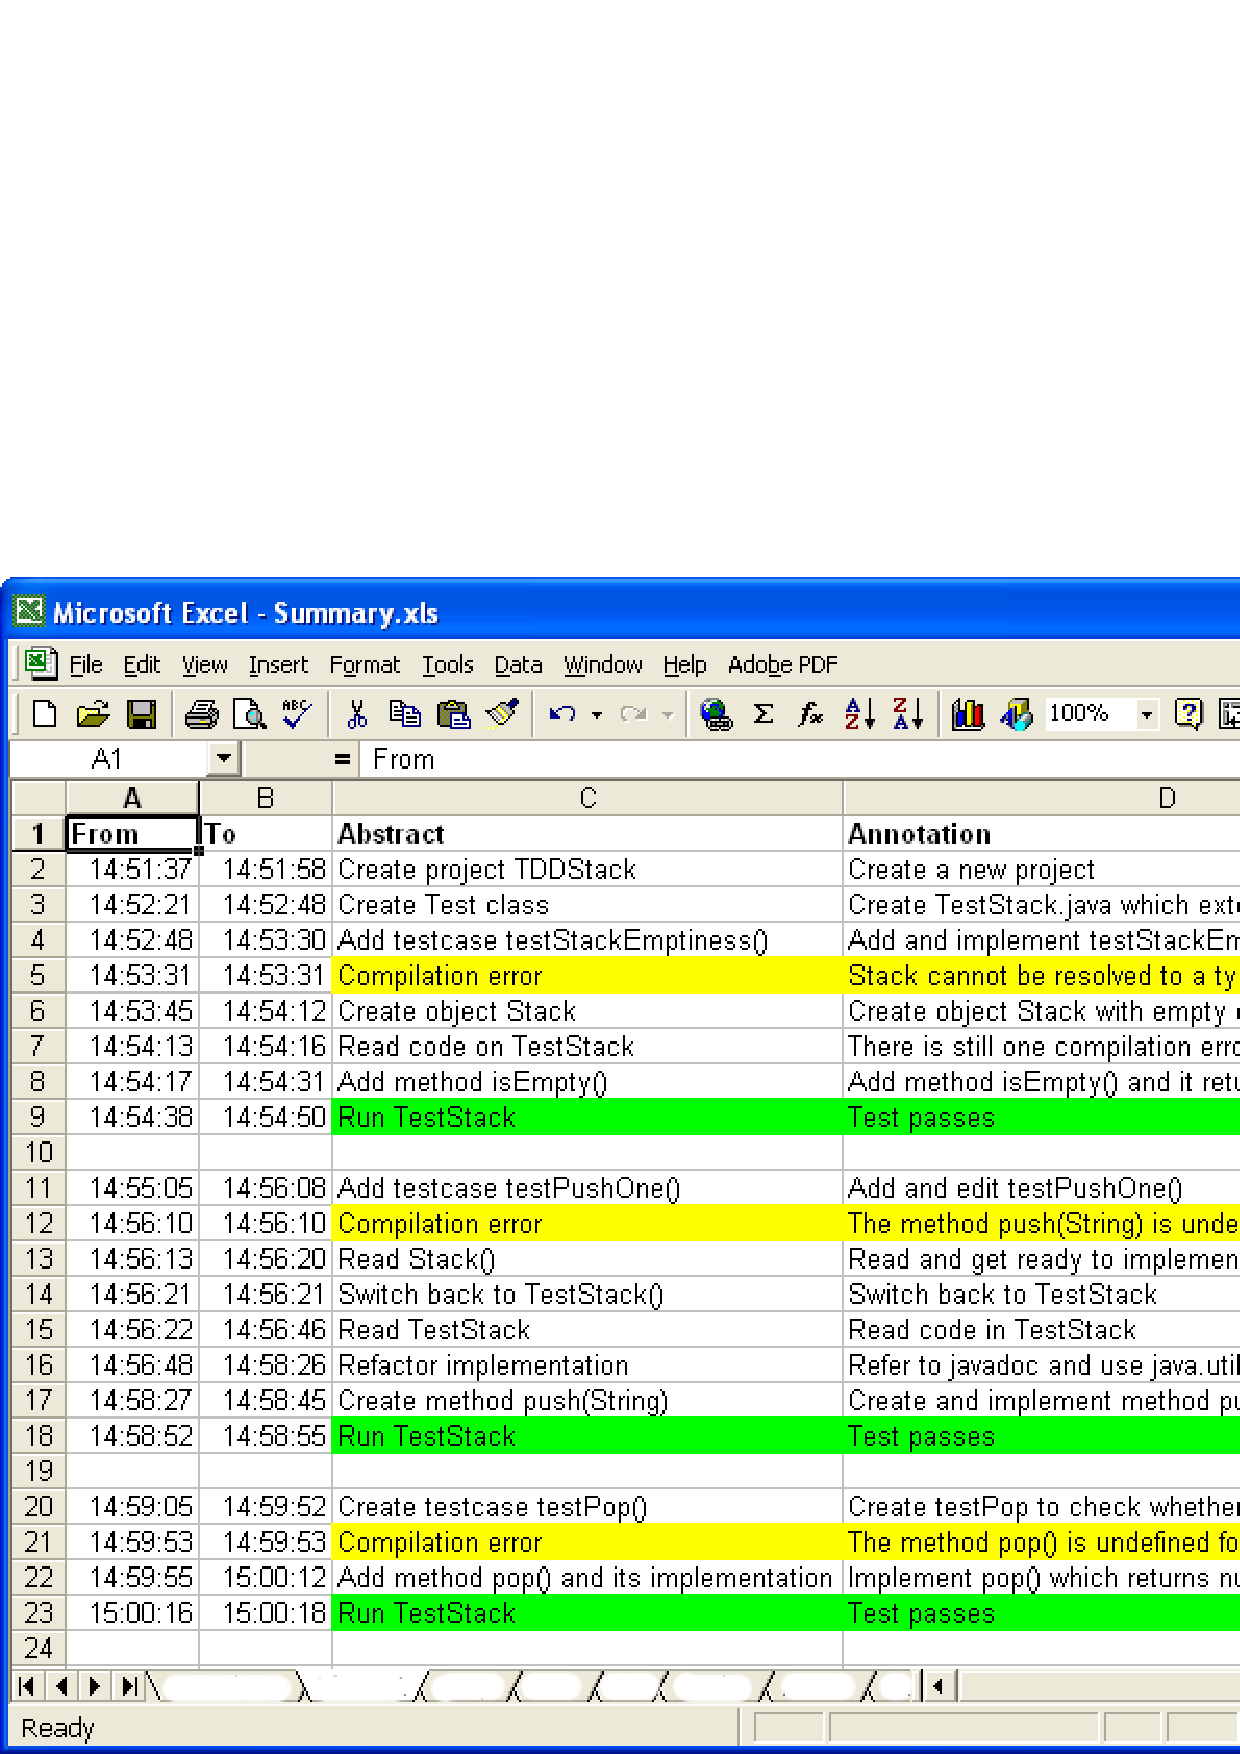
\includegraphics[width=0.8\textwidth]{figs/ESR-VideoScript}
  \caption{Observation Results in Excel}
  \label{fig:VideoExcelScript}
\end{figure}
As seen in Figure \ref{fig:VideoExcelScript}, activities such as compilations, failed test invocations and successful test invocations were highlighted in contrast to Zorro's TDD Development Stream analysis results as shown in Figure \ref{fig:gui}.

\subsection{Validation of Zorro's Data Collection}
\label{sec:Pilot-Validation-Collection}
I used activities observed from the ESR videos to validate Zorro's data collection. The comparison between activities recorded by ESR and activities collected by Zorro allowed me to perform a partial validation of Zorro by determining which activities were missed by Zorro and which activities were not correctly collected by Zorro. This section introduces the analysis method, followed by analysis results. 

\subsubsection{Validation Analysis Method}
After watching each participant's video, I compared the activities observed 
by me to activities collected by Zorro and presented by the TDD Development 
Stream analysis. Figure \ref{fig:DataVerification} illustrates the comparison 
for a participant. The sub-figure on the left is a screen-shot showing activities
collected by Zorro and the sub-figure on the right is the Excel spreadsheet with 
development activities I observed for a programming period. 
\begin{figure}[hbtp]  
  \centering
  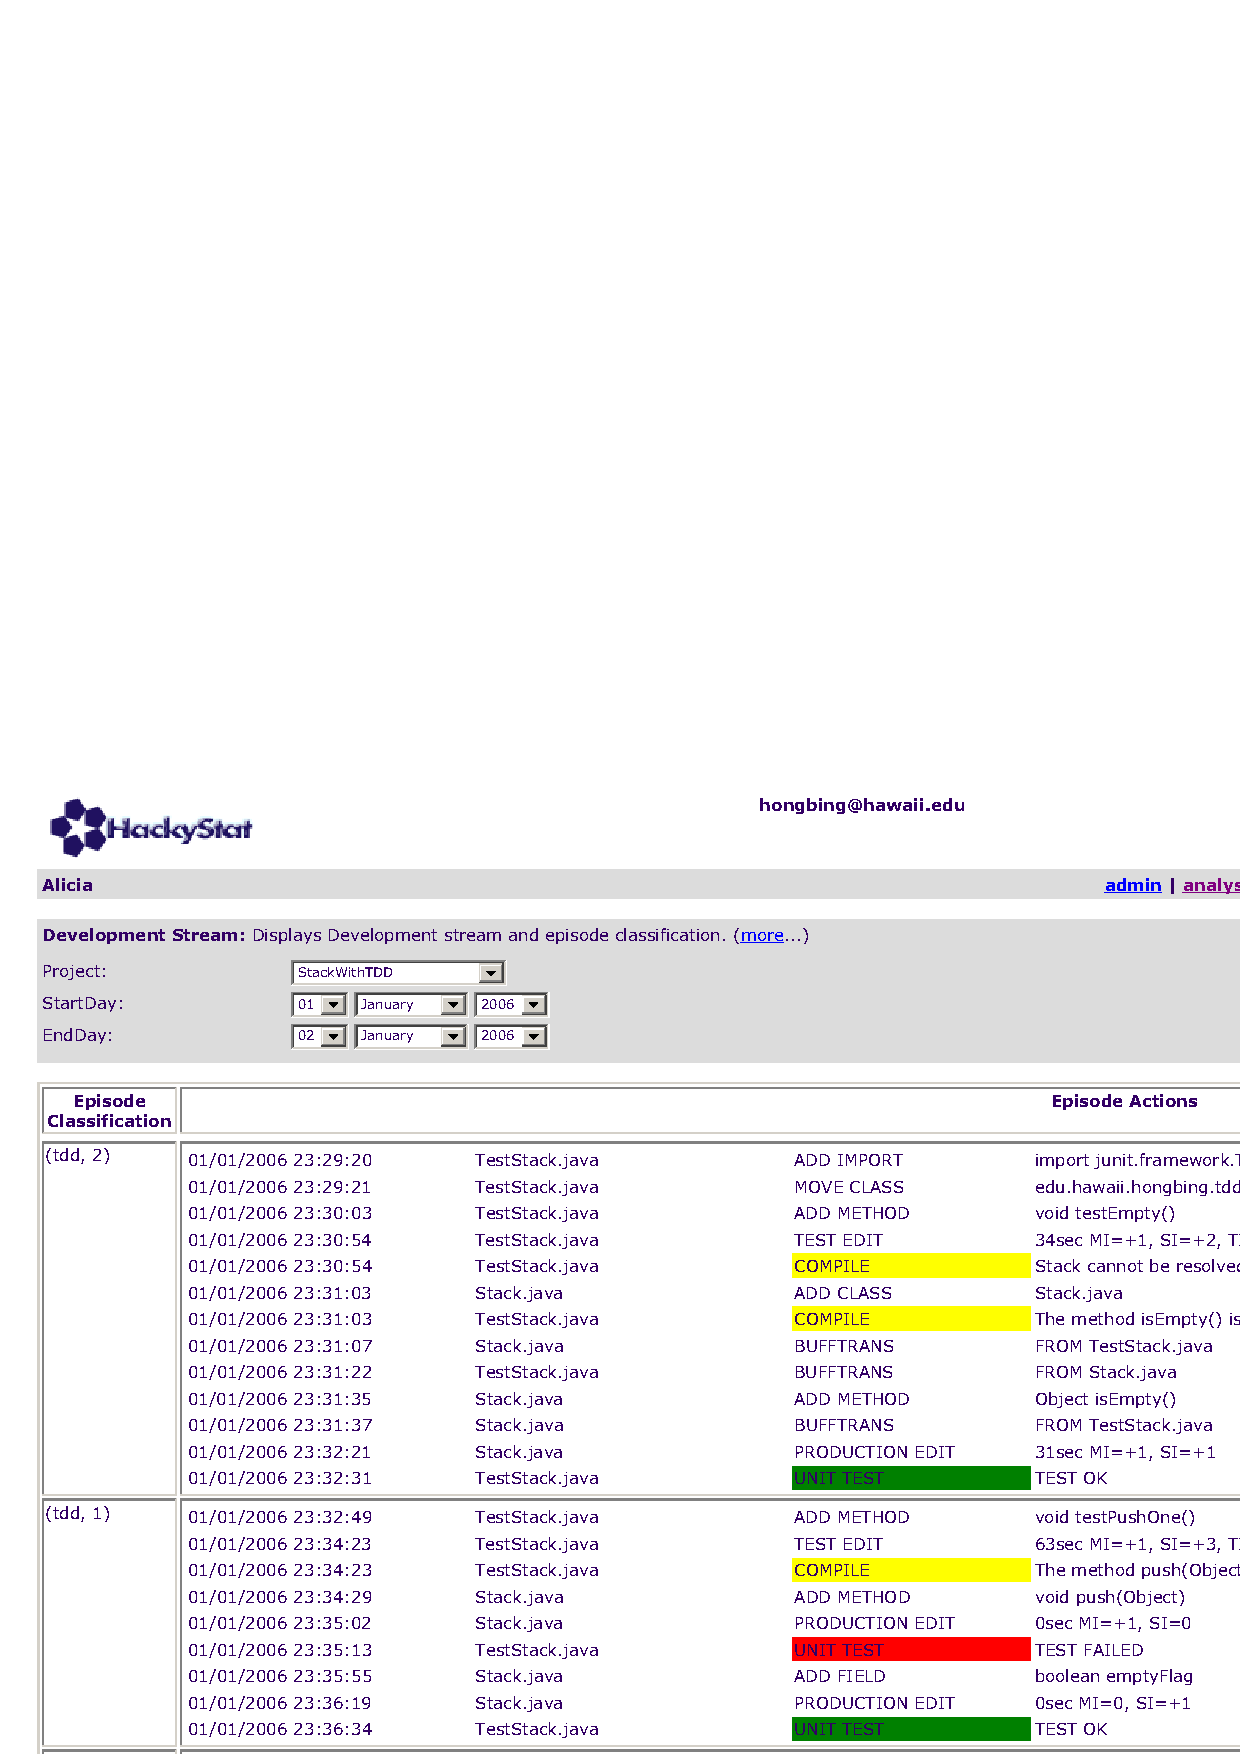
\includegraphics[width=0.48\textwidth]{figs/Zorro-Gui} 
  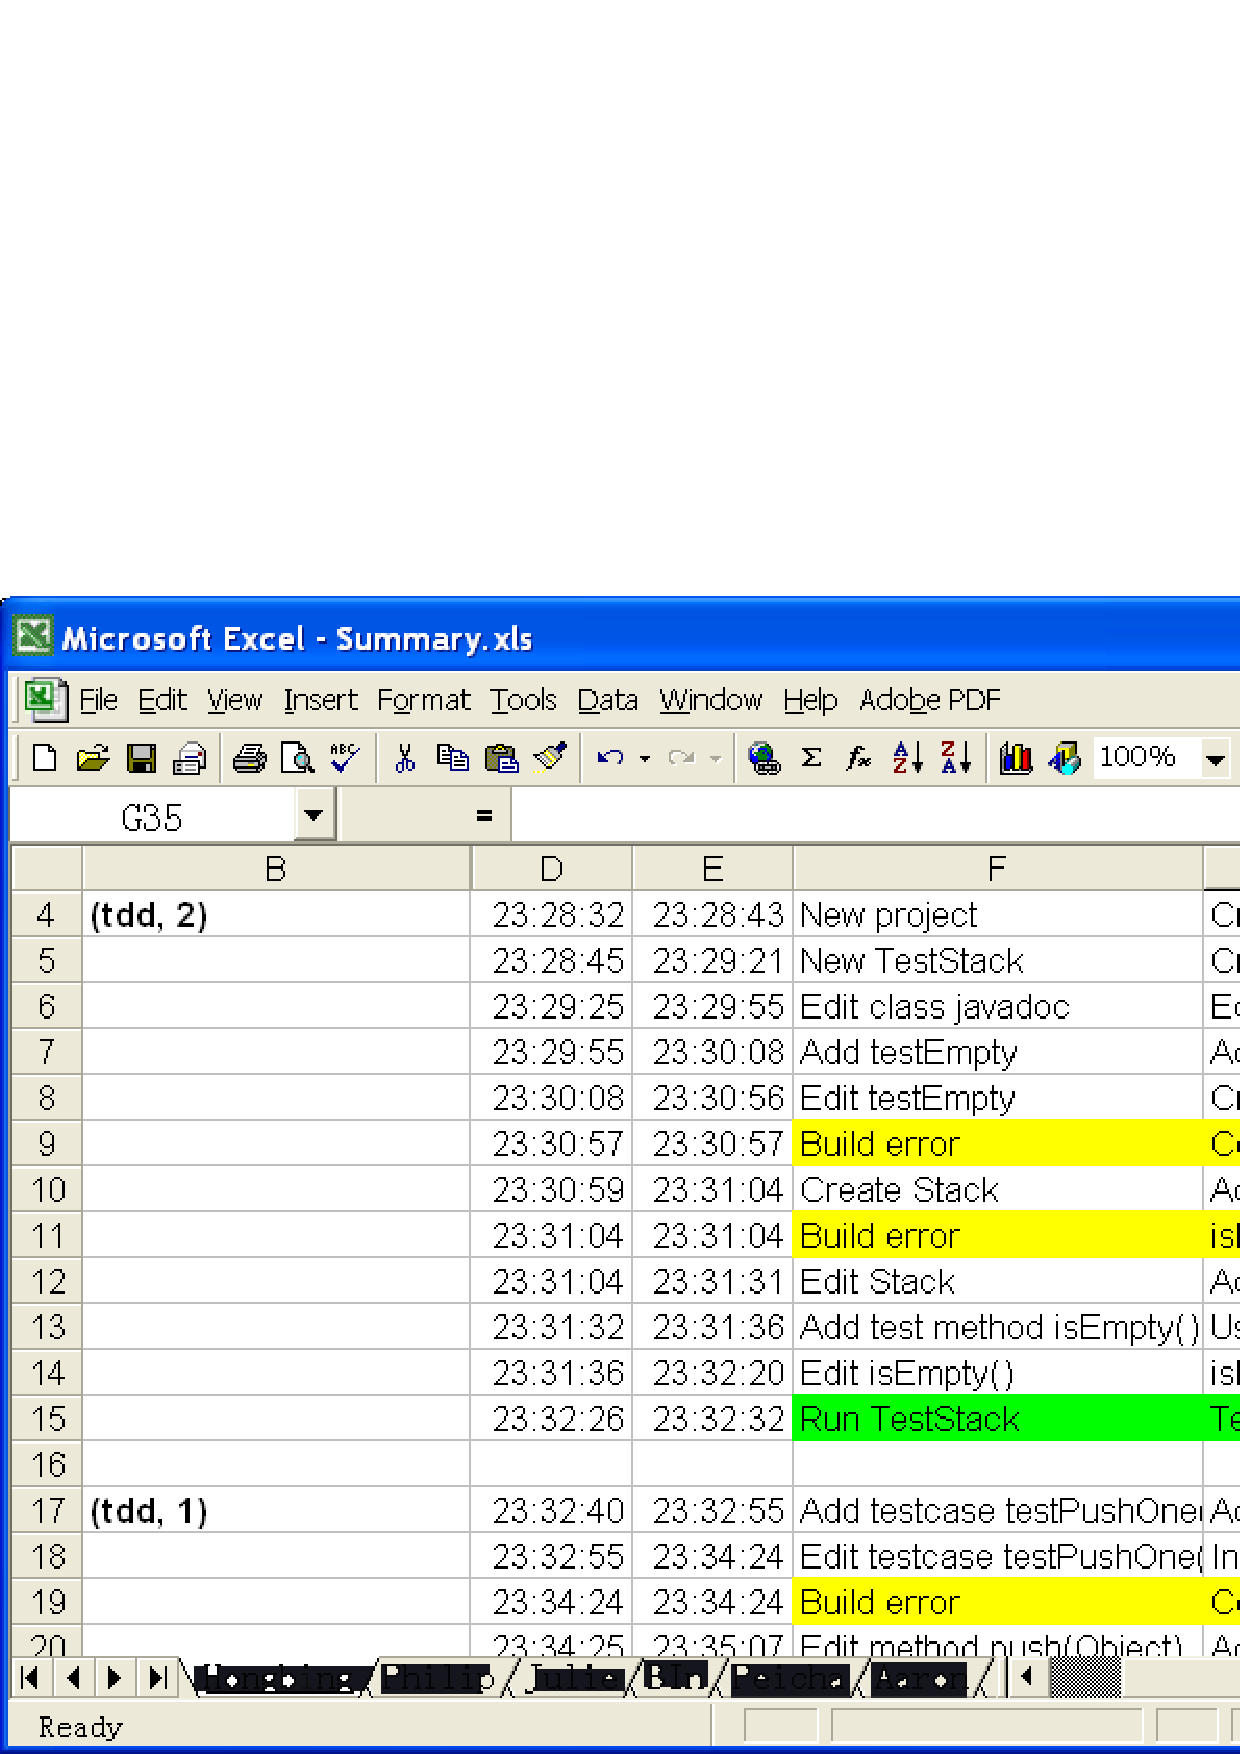
\includegraphics[width=0.48\textwidth]{figs/VideoScriptExcel}
  \caption{Comparison of Development Activities between Zorro and ESR}
\label{fig:DataVerification}
\end{figure}
Using this comparison method, I validated Zorro's data collection for
all of the development streams produced by pilot study participants. 
The next section presents this analysis result. 

\subsubsection{Validation Results}
Overall Zorro was capable of capturing development activities. Compared
to activities observed from ESR videos, Zorro collected almost all of 
them, and thus it was pointless to literally report number of missed and 
incorrectly collected activities. Instead, I decided to summarize types 
of missed and incorrectly collected activities that affected Zorro's inference. 
The following is a summary of problems I found with regard to Zorro's 
data collection:
\begin{itemize}
\item \textbf{Problem 1}: Insignificant editing work. 
  \begin{tabular}{lp{10cm}}
   Severity: &  \small\textit{High}\\
   Reason:   &  \small\textit{Editing work did not change object metrics such as 
                         statements and methods. Or developers quickly edited
                         code, which resulted in one state change event only.} \\ 
   Result:    & \small\textit{Episodes were misclassified since editing activities 
                              were not captured.} \\ 
   Resolution: & \small\textit{Change the implementation of file edit 
                           sub stream in SDSA to look for file size 
                           change as well.} \\ 
   Affected: &  \small\textit{6 episodes.}
  \end{tabular}

\item \textbf{Problem 2}: Missed compilation errors to test code.
  \begin{tabular}{lp{10cm}}
    Severity: & \small\textit{Medium}\\
    Reason:   & \small\textit{Changes to production code caused 
                compilation errors to inactive test code.} \\
    Results: & \small\textit{Episode were misclassified.} \\
    Resolution: & \small\textit{Fix the Hackystat Eclipse sensor to report 
                  compilation errors on inactive files as well.}\\
    Affected: & \small\textit{2 episodes}
  \end{tabular}

\item \textbf{Problem 3}: Two unit test invocations were grouped
together or one unit test invocation was divided into two continuous
episodes.
  \begin{tabular}{lp{10cm}}
    Severity: & \small\textit{Medium}\\
    Reason: & \small\textit{Eclipse sensor collected multiple data 
              entries for one test invocation.}\\
    Results: & \small\textit{Two or more episodes were grouped 
               together or divided resulting that they were not 
               classified correctly.} \\
    Resolution: & \small\textit{Tag unit tests with run time to 
                  group multiple unit test entries belong to 
                  one test invocation together.} \\
    Affected: & \small\textit{3 episodes}
  \end{tabular}
\end{itemize}

Of the three problems listed above, one was high and the other two 
were medium in severity. In total, they affected 11 out of 92 
episodes. 

\subsection{Validation of Zorro's TDD Behaviors Inference}
\label{sec:Pilot-Validation-Inference}
As seen in Figure \ref{fig:DataVerification} and Table \ref{tab:ZorroPilotStudy}, 
Zorro inferred development behaviors as ``TDD'', ``Refactoring'' or 
``Test-Last''. For each behavior category, Zorro also defined sub-types 
as seen in Figure \ref{fig:DataVerification}, but I will not discuss them 
in this analysis because sub-types are for Zorro's internal uses only. In 
this analysis, I compared development behaviors I observed in ESR videos 
to development behaviors inferred by Zorro.

\subsubsection{Validation Analysis Method}
In Section \ref{sec:Pilot-Observation}, I introduced how I did participant 
observation using videos. After observing low-level development activities, 
I played the videos again to derive development behaviors of TDD. The remark 
in a yellow background at the top-right corner of Figure \ref{fig:EsrVideo} 
was a visual presentation of my derivation of development behaviors. In this
data analysis, similar to what I have done in Section 
\ref{sec:Pilot-Validation-Collection}, I compared the development behaviors 
derived from ESR videos to development behaviors inferred by Zorro for validation. 

\subsubsection{Validation Results}
Table \ref{tab:EsrPilotStudy} is a summary of the validation results. For each
participant, it lists number of total, classified and wrongly classified
episodes along with the percentage of classification errors. 
\begin{table}[htbp]
\centering
  \caption{TDD Development Behavior Validation}
  \begin{tabular}{|r|r|r|r|r|r|r|}
  \hline
    Subject ID & Episode & Classified & Wrongly Classified & Percentage \\ \hline
    1          & 15 &  14 &  2 & 13.3\% \\ \hline
    2          & 13 &  13 &  3 & 23.3\% \\ \hline
    3          & 14 &  14 &  1 &  7.1\% \\ \hline
    4          & 14 &  14 &  1 &  7.1\% \\ \hline
    5          & 16 &  11 &  1 &  9.1\% \\ \hline
    6          & 11 &  11 &  1 &  9.1\% \\ \hline
    7          &  9 &   9 &  1 & 12.5\% \\ \hline \hline
    Total      & 92 &  86 & 10 & 11.6\% \\ 
  \hline
  \end{tabular}
  \label{tab:EsrPilotStudy}  
\end{table}
According to Table \ref{tab:EsrPilotStudy}, 11.6\% of episodes 
were wrongly classified. On the other hand, it indicated  that Zorro 
inferred TDD behaviors correctly for 88.4\% of episodes.

In addition, the validation analysis helped me to discover an inference 
problem for very long episodes that occurred when developers did not 
invoke unit tests frequently. It is described in the following:
\begin{itemize}
\item {\textbf{Problem 4}: An episode had too many activities.
  \begin{tabular}{lp{10cm}}
    Severity: & \small\textit{Low}\\
    Reason: & \small\textit{Participants did not invoke unit testing 
              frequently enough.}\\
    Results: & \small\textit{Episodes were misclassified.}\\
    Resolution: & \small\textit{Introduce long episode type and 
                  avoid inferring episode with too many activities.} \\ 
    Affected: & \small\textit{2 episodes}
  \end{tabular}}
\end{itemize}
This behavior is clearly a violation to TDD's short-duration 
characteristic, but Zorro did not have an episode behavior category 
for it when I conducted the pilot study. Later I included this behavior 
in the new development behavior classification schema in current 
version of Zorro (See Chapter \ref{ch:Zorro}).

\section{Research Conclusions}
The above analyses show that the one-shot case study research strategy is useful for Zorro validation. ESR, an Eclipse screen recording tool, is capable of recording incremental small changes made by participants for the purpose of participant observation. Although ESR caused a small delay when it was initialized, participants did not notice much delay in the pilot study. With ESR videos, I was able to validate both Zorro's data collection and TDD behaviors inference. Thus, ESR is suitable for Zorro validation studies and the research question Q1a is answered. 

\begin{comment}
Participants in this study spent 28 to 66 minutes on the
programming task using TDD. Zorro partitioned the overall development
efforts into 92 episodes, out of which 86 were classifiable; 6 were
unclassifiable. It classified 76 out of 86 episodes correctly
resulting in classification accuracy rate 88.4\%.
\end{comment}

%result demonstrates that Zorro has the potential to 
%understand developer's TDD development behaviors automatically 
%using low-level development activities. 
Using videos recorded by ESR for participant observation, I found that Zorro had 3 types of solvable data collection problems. The validation analysis of Zorro's data collection shows that Zorro can collect sufficient low-level development activities accurately for the purpose of TDD development behavior inference. This supports the research question Q1b. 

Only two out of 93 episodes were incorrectly inferred by Zorro because they had too many activities in them. Other than this, Zorro's inference rules recognized TDD development behaviors correctly when low-level development activities were sufficient. Thus this pilot study provides the supporting evidence to research question Q1c. 

\section{Discussion and Zorro Improvements}
In a simple environment setting, I validated that Zorro worked well at collecting low-level development activities and inferring developer's TDD behaviors. However, as described above, this pilot study also identified several areas that could be improved. 

\subsection{Data Collection}
Section \ref{sec:Pilot-Validation-Collection} addressed three data collection problems that prevented Zorro from inferring TDD behaviors correctly. Following the pilot study, I fixed them in the current version of Zorro.

\subsection{TDD Behaviors Classification}
The validation analysis in Section \ref{sec:Pilot-Validation-Inference} showed that applying inference rules on episodes that had too many development activities caused inference errors. More interestingly, about 50\% of episodes were ``Test-Last'' in the pilot study. There are several possibilities that could explain this phenomenon. One possibility could be that the programming problem (Stack) is too simple and developers did not need to fail tests first to have the correct implementation. Another possibility could be that Beck's concise summary of TDD is just too simple, while real TDD development is much more complicated than what he described. For instance, a developer can add a new test that does not fail initially because the functional code works well even without any change. This development behaviors is none of ``TDD'', ``Refactoring'' and ``Test-Last''. Therefore, after the pilot study, I developed a much sophisticated TDD behaviors classification schema as seen in Table \ref{tab:Zorro.Categories} that can best describe real development behaviors. The long episode behavior is part of this schema. 

\subsection{Process Conformance Inference}
In the pilot study, I did not directly calculate process conformance of TDD. Instead, I used development behaviors to describe process conformance: ``TDD'' and ``Refactoring'' behaviors were TDD conformant automatically while ``Test-Last'' was not. According to this simple measurement and Table \ref{tab:ZorroPilotStudy}, in the pilot study, only less than 50\% (40 out of 92 episodes) of episodes were TDD conformant, which was very contrary to what I had anticipated before the study. Further research indicated that this simple measurement was very limited. 

With the introduction of the new episode classification schema, I defined a more sophisticated two-step model for process conformance of TDD (See Figure \ref{fig:heuristic}) using heuristics. The first step is to infer development behaviors in episodes and then look up episode context to determine their process conformance.
\begin{figure}[htbp]
  \centering
  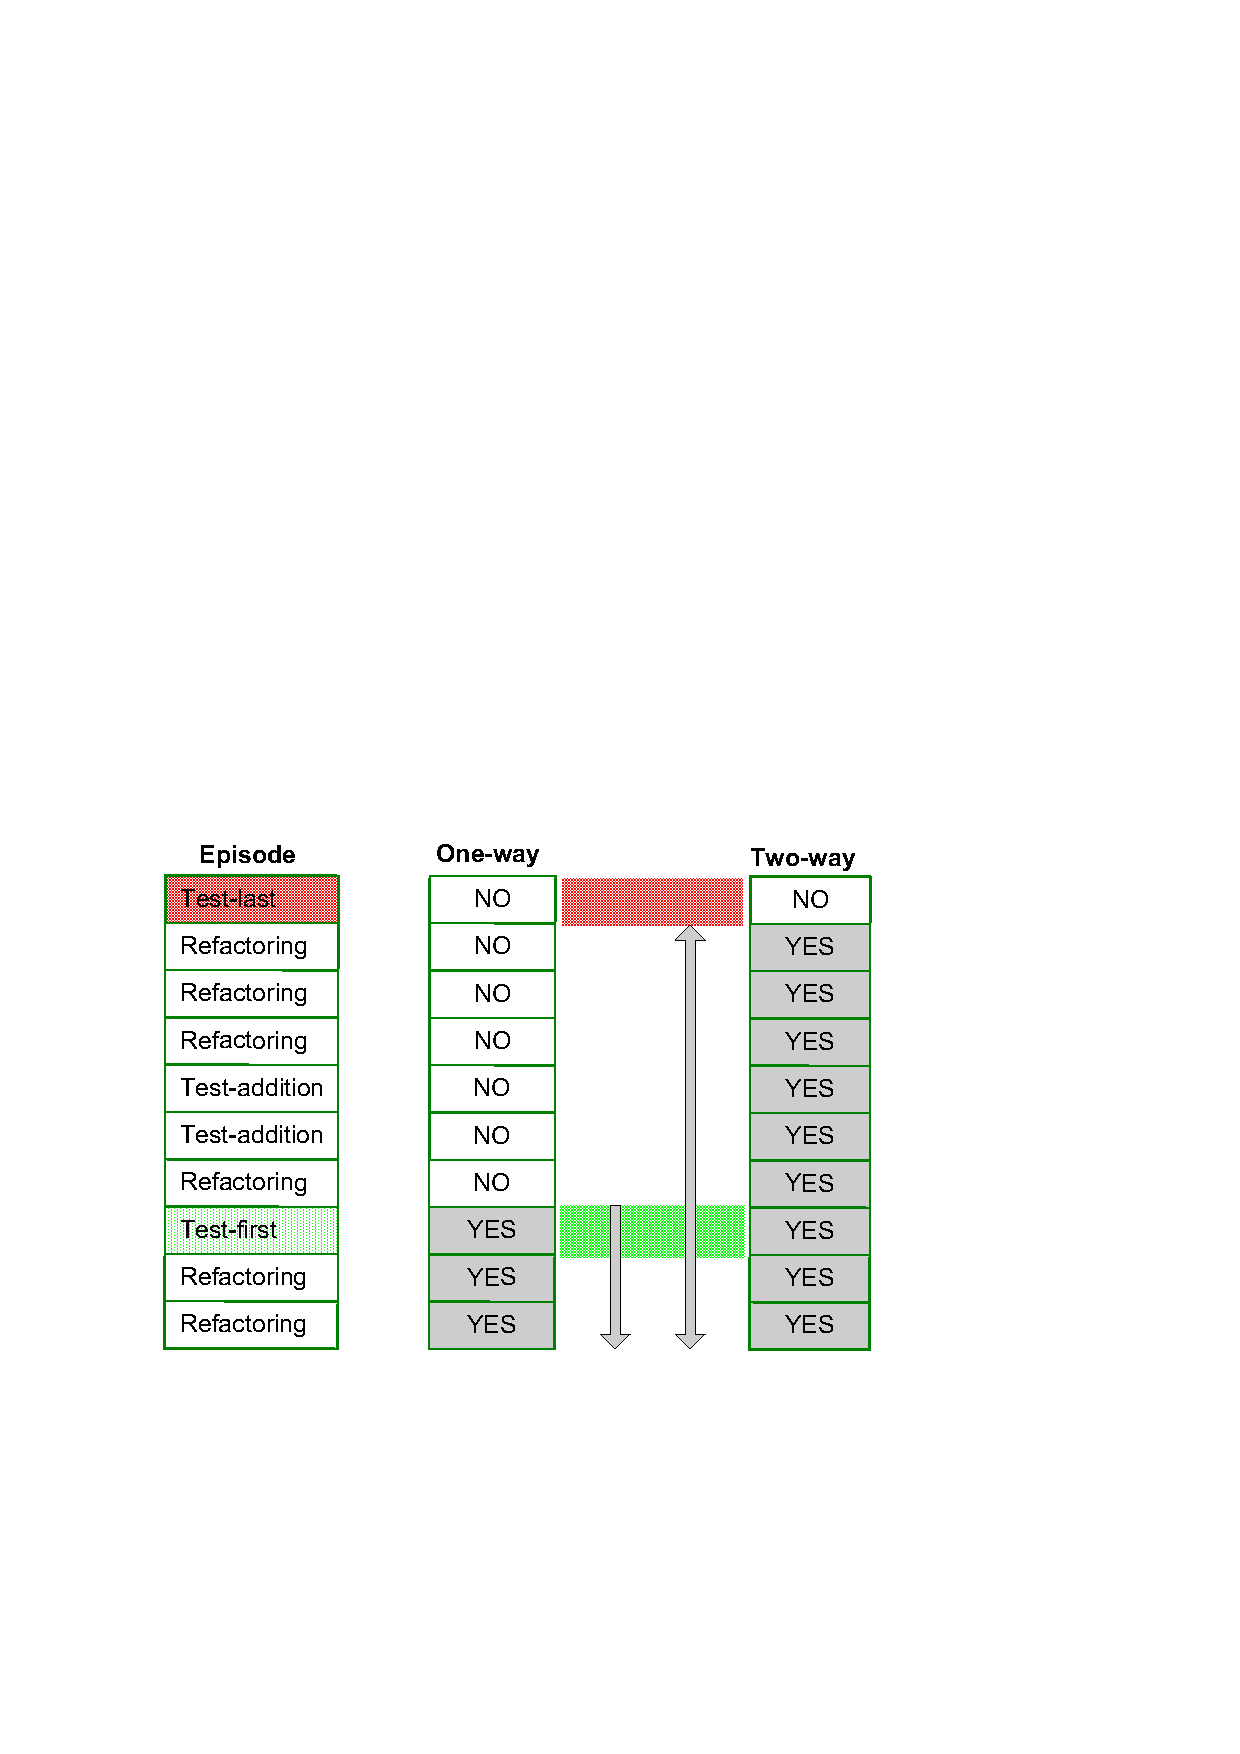
\includegraphics[width=0.8\textwidth]{figs/HeuristicAlgorithms}
  \caption{Heuristic Algorithms of TDD Conformance}
  \label{fig:heuristic}
\end{figure}
There are three lists in Figure \ref{fig:heuristic}. The left-most one is a list of development behaviors recognized by Zorro's inference rules. As their names indicate, the episodes can be ``test-first", ``test-addition", ``refactoring", or ``test-last" etc. The one-way and two-way TDD heuristic algorithms are on the right side of Figure \ref{fig:heuristic}. The one-way algorithm uses look-forward approach to determine whether an episode is TDD conformant, while the two-way heuristic algorithm uses both look-forward and look-backward approaches. Figure \ref{fig:heuristic} indicates this difference using a single-head arrow and a double-head arrow. I implemented these heuristic rules with the support of JESS \cite{Friedman-Hill:03}. Section \ref{sec:Zorro-TDDConformance} in Chapter \ref{ch:Zorro} has a detailed description to this heuristic. Our preliminary work suggests that the two-way heuristic algorithm can understand real world situations better than the one-way algorithm.

\section{Chapter Summary}
This chapter introduced the pilot study, a test to investigate how to validate Zorro using participant observation supported by ESR. The study showed that Zorro's data collection and TDD behaviors inference can be validated by analyzing development videos recorded by ESR. This study also identified several problems that helped to improve Zorro. With these improvements, I conducted an extended classroom case study following the pilot study in my thesis research. 
\chapter{Classroom Case Study}
\label{ch:Classroom}
Following the pilot study and collaborative research with Dr. Hakan Erdogmus\footnote{Dr. Hakan Erdogmus is a Senior Research Officer in the NRC-IIT Software Engineering Group (http://iit-iti.nrc-cnrc.gc.ca/personnel/erdogmus\_hakan\_e.html). He has interests in Software Economics, Agile Software Development, and Software Process Measurement and Awareness.},  I improved Zorro and conducted an extended validation study in the software engineering classes at the University of Hawaii in Fall 2006. This study shows that Zorro can collect low-level development activities and infer TDD development behaviors accurately. This study also provides evidence that Zorro is helpful for beginners who do not have much prior experience with the TDD practice. 

\begin{comment}
The classroom case study is an evaluation designed to evaluate Zorro's low-level development activity collection and automated inference of Test-Driven Development behaviors. This chapter has three sections. Section \ref{sec:CaseStudyMethod} explains the analysis method for individuals using the first participant's data. Section \ref{sec:CaseStudyFindings} presents the summary of analysis results over all participants' data. In the end Section \ref{sec:discussion} discusses the research findings from this research. The pilot study of Zorro was a success. It convinces us that Zorro's rule-based approach has promise for developer's TDD behavior inference. It also demonstrates that the research methodology works. Following this study, I fixed several data collection problems found in the pilot study. We also improved Zorro's TDD inference rules based on the pilot study and collaboration with Software Engineering Group at the National Research Council of Canada.
\end{comment}

\section{Purpose of the Study}
The purpose of this study was to validate Zorro using the case study research method tested by the pilot study (Chapter \ref{ch:Pilot}) and investigate how useful Zorro is for TDD beginners. 

\begin{comment}
Currently Zorro collects development activity data more accurately,
has a more sophisticated episode classification schema, and infers
developer TDD behaviors based not only on the episode's internal
structure but also the context in which the episode occurred.
The purpose of this study is to:
\begin{enumerate}
\item perform Zorro validation study using the Eclipse Screen Recorder;
\item perform a second type of validation in which participates
provide feedback through the web-based validation wizard of Zorro;
\item obtain feedback regarding whether Zorro can help TDD
beginners through a post-test interview.
\end{enumerate}
\end{comment}

\section{Research Questions}
The specific research questions for the classroom case study were:
\begin{itemize}
\item{Q2a: Does Zorro collect software development activities accurately enough for episode partitioning and TDD behavioral inference?}
\item{Q2b: Does Zorro's inference of TDD behaviors agree with analyses based upon participant observation?}
\item{Q2c: Does Zorro's inference of TDD behaviors agree with what participants believe to be their TDD behaviors?}
\item{Q2d: Does Zorro provide useful information for beginners to understand TDD and improve their TDD development?}
\end{itemize}

Research questions Q2a, Q2b, and Q2c are three specific research questions for the thesis research question Q1, ``\textit{Can Zorro automate the recognition of TDD behaviors using automatically collected software metrics?}''. The research question Q2d corresponds to the thesis research question Q2, ``\textit{How useful is Zorro?}'' 

\section{Experiment Design}
\label{sec:ClassroomDesign}
To address the above research questions, I used the one-shot case study research method as in the pilot study. TDD was the treatment. We taught TDD to participants and asked them to develop software using TDD in this study. 

\subsection{Participants}
TDD beginners were the targeted population. I recruited participants from a senior-level software engineering class and a graduate-level software engineering class, both of which were taught by Professor Philip Johnson in Fall 2006 at the University of Hawaii. There were 16 students in two classes and 11 of them agreed to participate in this study. 

\subsection{Materials}
I conducted this study in the Collaborative Software Development Laboratory (CSDL) at the University of Hawaii. Three Windows-based lab computers were used, one of them acted as a Hackystat server and the other two were used by participants to develop software for this study. I configured two development computers with necessary software including JDK, Eclipse, the Hackystat Eclipse Sensor, QuickTime and ESR. Bowling Score Keeper, a famous problem that has been widely used in empirical evaluation research of TDD\cite{George:03,Erdogmus:05}, was the programming task. Since participants were TDD beginners, I designed user stories in plain text (Appendix \ref{app:UserStoriesBSK}) to help them develop the program without needing prior experience with the game. Since user stories are ordered from the easiest one to the hardest one, they can also be used as the ``To Do'' list for TDD development.  

\subsection{Instruments}
I instrumented the development processes with the Hackystat Eclipse sensor and ESR. Prior to the study, I created a Hackystat key for each participant and configured the Hackystat Eclipse sensor for him/her. At the beginning of the study, I asked participants to enable ESR so that it would record their development processes. Participants validated Zorro's TDD behavioral inference using the ``TDD Episode Validation'' (Figure \ref{fig:EpisodeFeedback}) analysis. The ``Web Validation Wizard'' was another instrumentation tool that I used to collect participant's evaluation. Additionally I interviewed participants in the study and recorded the interviews using a digital voice recorder.

\subsection{Procedure}

This experiment included a TDD lecture and a 2-hour lab session. 

\begin{enumerate}
\item{TDD Lecture}

In both software engineering classes, Professor Philip Johnson gave the same TDD lecture to students. The lecture included following contents:
\begin{itemize}
\item Introduction to TDD
  \begin{itemize}
  \item Two principles of TDD from \cite{Beck:03}
  \item Red/green/refactor pattern of TDD
  \item TDD Rhythm \cite{TDDRhythm}
  \item TDD vs. Unit Testing
  \item A TDD example: implementing stack by writing test first 
  \end{itemize}
\item Why TDD?
  \begin{itemize}
    \item{Developer gets quick feedback.}
    \item{TDD improves software quality.}
    \item{TDD promotes simple design.}
    \item{Microsoft has successful story on TDD \cite{Bhat:06}}
    \item{Test-Driven Development proves useful at Google\cite{RoyOsheroveBlog}}
  \end{itemize}
\item About TDD
  \begin{itemize}
    \item{TDD may not be appropriate for everybody.}
    \item{TDD is about design.}
    \item{Some studies show that TDD improves software quality.}
    \item{TDD may reduce productivity.}
    \item{TDD references including testdriven.com, mailing list and blogs.}
  \end{itemize}
\item Reading and programming assignments
  \begin{itemize}
    \item {Page 1-20 of Beck's book ``Test-Driven Development by Example'' \cite{Beck:03}}
    \item {TDD Quick Reference \cite{TDDQuickReference}}
    \item {Practice TDD on Roman Numeral Problem (Appendix
    \ref{app:UserStoriesRomanNumeral})}
  \end{itemize}
\end{itemize}

After the lecture, students practiced TDD by working on an in-class assignment, the Roman Numeral Conversion (Appendix \ref{app:UserStoriesRomanNumeral}). Then they were asked to voluntarily participate in this study. The study was conducted in CSDL under my supervision. The 2-hour lab session included 90-minute of development using TDD, Episode Validation, Participant Interview and Zorro Usefulness Evaluation. 

At the beginning of the study, I introduced the purpose and content of this research study to participants, followed by the consent form signing. Then I gave them user stories of the Bowling Score Keeper problem (Appendix \ref{app:UserStoriesBSK}) and explained that they only needed to spend 90 minutes on the programming task. Following a five minute introduction, I asked them to start up Eclipse, enable the ESR recorder and begin programming. 

\item{TDD Development (90 minutes)}

Each participant developed a program to compute bowling game scores in TDD following the provided user stories. I suggested that they use the user stories as a To-Do list to help them develop in TDD. The time limit was 90 minutes. It was acceptable if they did not finish all user stories by the end within the 90 minutes. 

\item{Validating Zorro's Inference about Their TDD Behaviors (15 minutes)}

After 90 minutes of development in TDD, participants exited Eclipse, which forced the Eclipse sensor to send all remaining development activities to the Hackystat server and stopped the ESR recorder. Following a five minutes coffee break, I then directed them to login into the Hackystat server and asked them to invoke the ``TDD Episode Validation'' (Figure \ref{fig:EpisodeFeedback}) analysis in which they provided their feedback to Zorro's inference results. As seen in Figure \ref{fig:EpisodeFeedback}, they commented on Zorro's inference of development behaviors and compliance to TDD. 

%they will use the Zorro evaluation wizard to analyze their TDD development and validate Zorro's TDD behavior inference (Figure \ref{fig:EpisodeFeedback}).

\item{Interview (5 minutes)}

I conducted an interview with each participant after he/she finished reviewing Zorro's inference of their development behaviors. The interview lasted 5 minutes. In the interview, I asked  participants questions regarding their development experiences on software engineering best practices, unit testing, TDD and software quality. 

\item{Zorro Usefulness Evaluation (10 minutes)}

At the end of the lab session, participants conducted several analyses using the ``Evaluation Wizard'' (Figure \ref{fig:EvaluationWizard}) provided by Zorro to evaluate its usefulness. 
\begin{figure}[htbp]
  \centering
  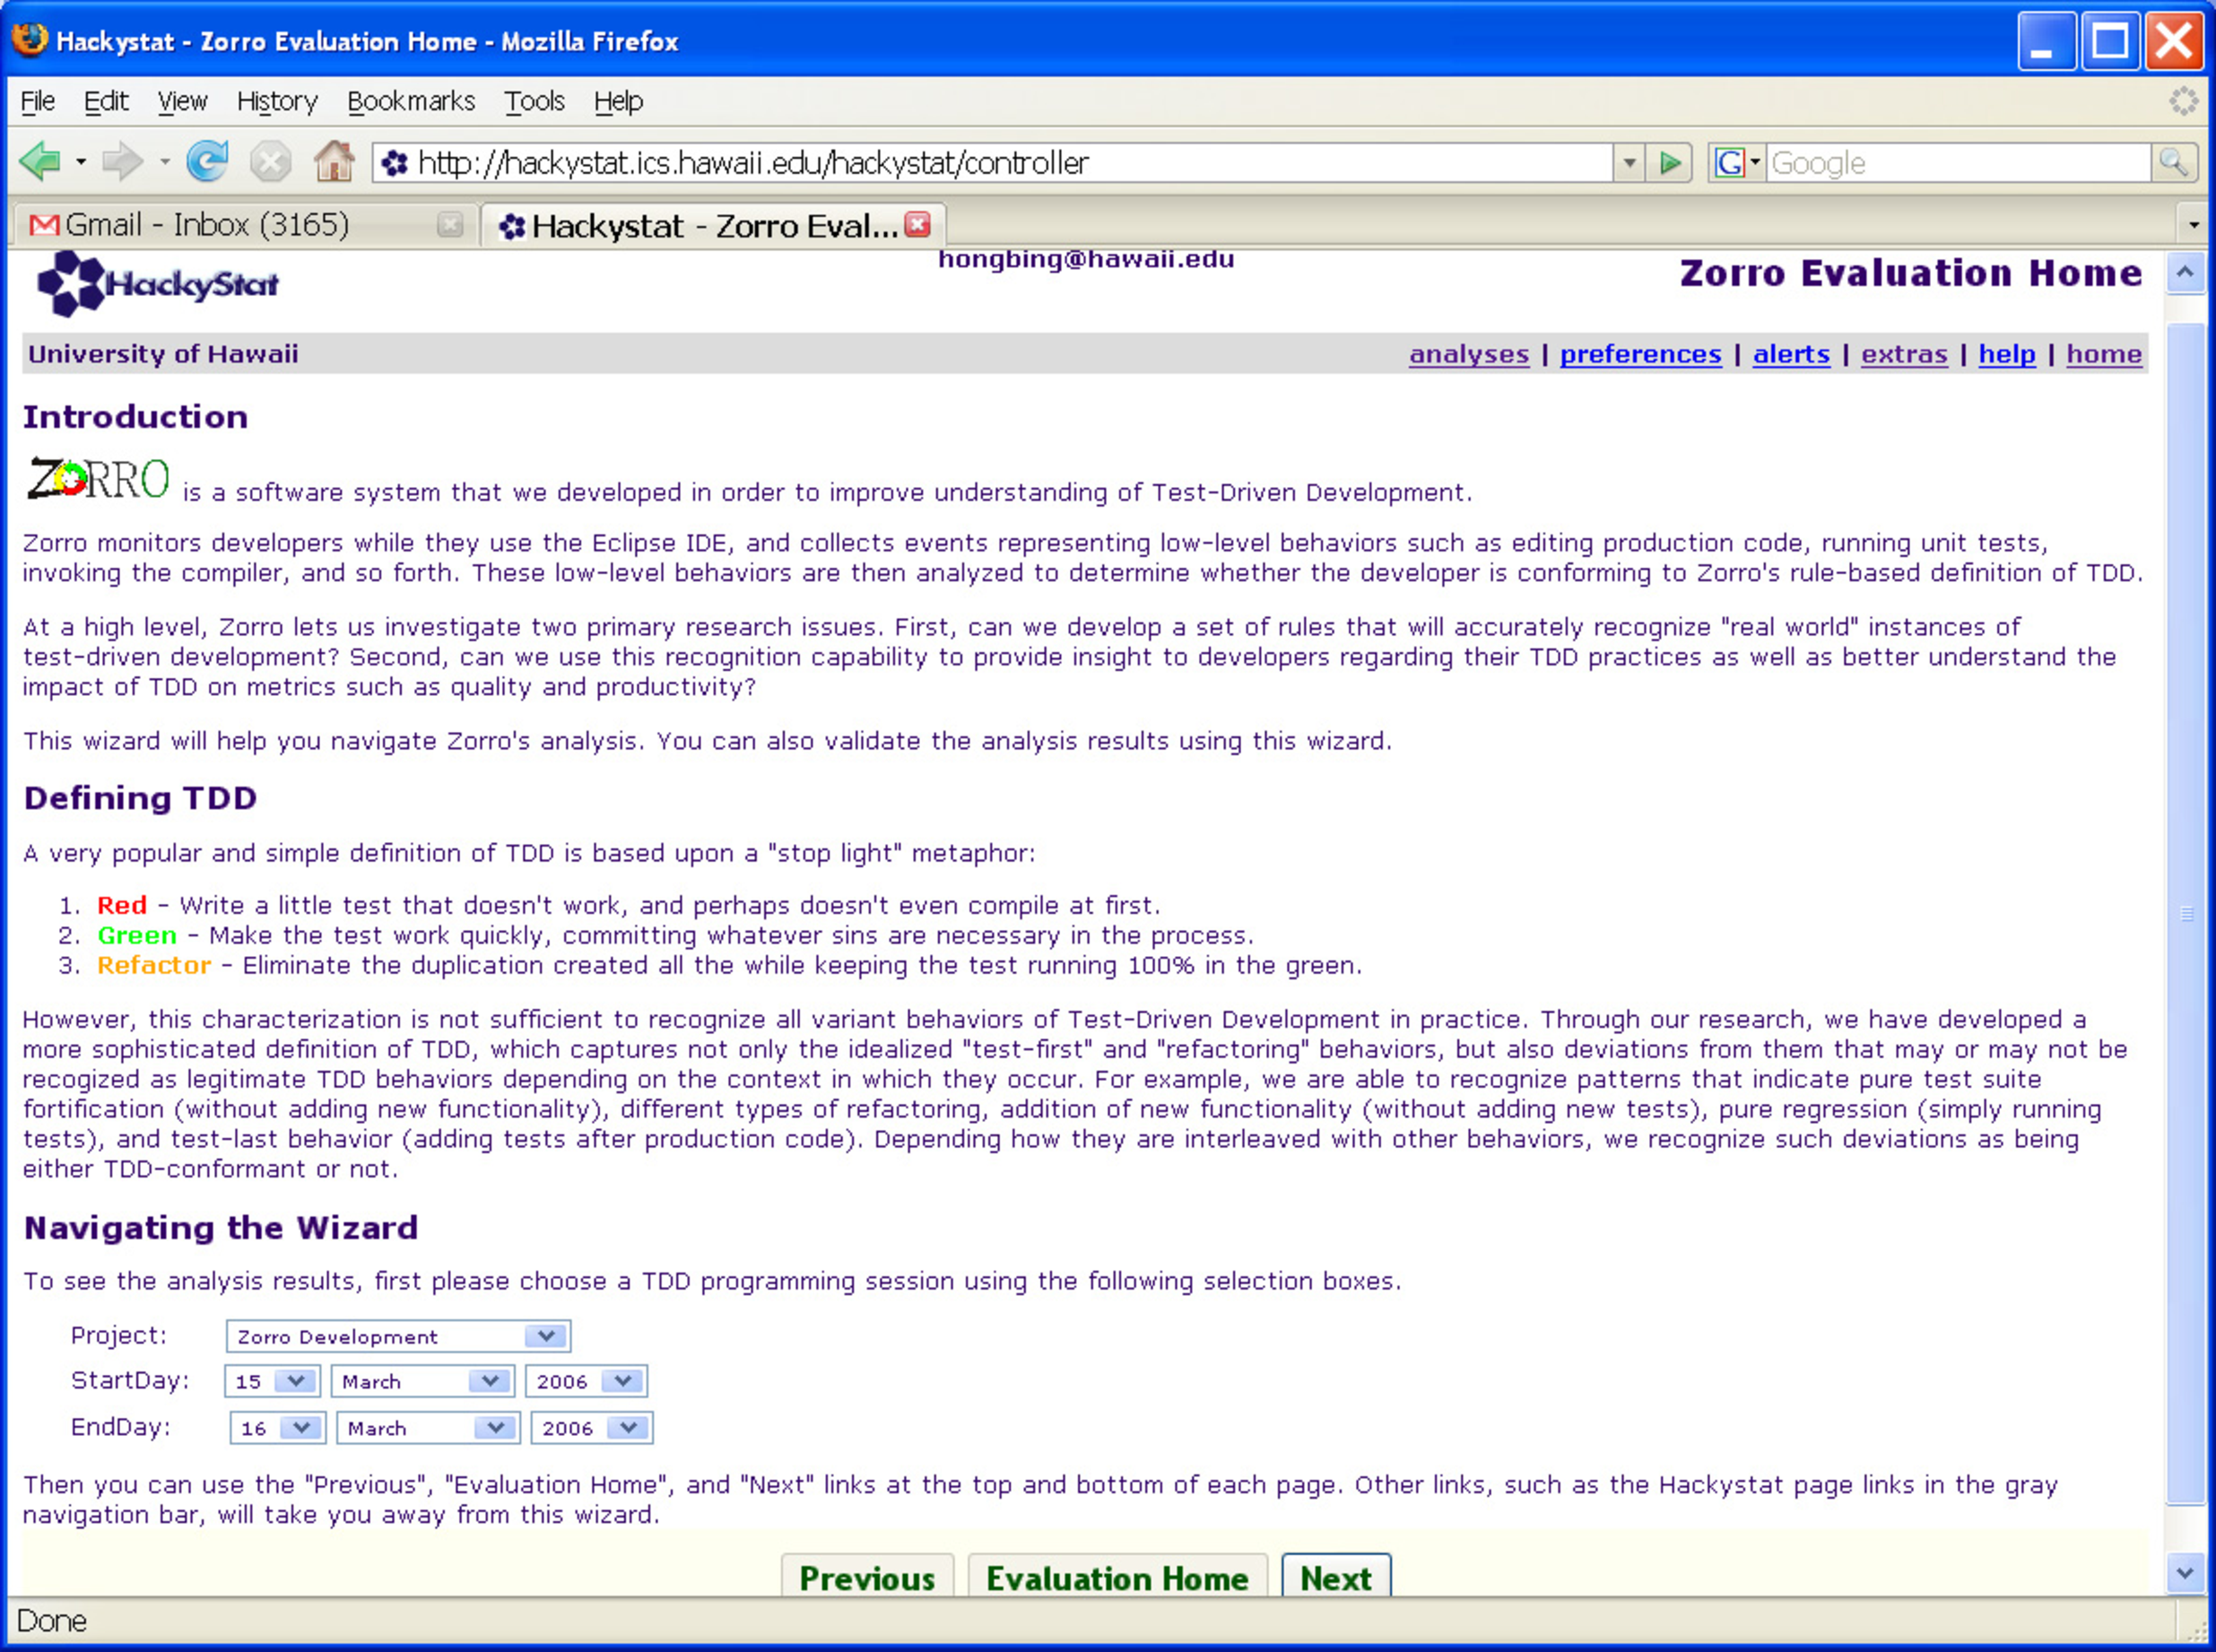
\includegraphics[width=0.8\textwidth]{figs/EvaluationWizard}
  \caption{Zorro Evaluation Wizard}\label{fig:EvaluationWizard}
\end{figure}
Participants used the wizard to review five analyses that were created based on Zorro's inference: Episode Demography, T/P Effort Ratio, T/P Size Ratio, Episode Duration and Episode Duration Bin. 

%, each participant took a 5 minutes coffee break before the interview started. The interview lasted 15 minutes during which I asked questions regarding the participant's experiences and opinions on unit testing, TDD and software quality. 

%In the end I will interview participants. The purpose of this interview is to learn participant's opinions on unit testing and TDD, discover questions and problems they may have, and investigate whether and how Zorro can help TDD beginners. The interview protocol and outline are available at Appendix \ref{app:CaseStudyInterviewGuide}.

\end{enumerate}

\subsection{Data Collection}
\label{sec:Classroom-DataCollection}
Similarly to the pilot study, I collected development activities using the Hackystat Eclipse sensor and development process videos using ESR. Development activities were saved on the Hackystat server, and ESR videos were saved on the lab PCs. To collect participants' validation comments, Zorro provides the ``TDD Episode Validation'' analysis (Figure \ref{fig:EpisodeFeedback}), which is an extension to the ``TDD Development Stream'' analysis (Figure \ref{fig:gui}) discussed in Section \ref{sec:Pilot-Analysis}. 
\begin{figure}[htbp]
  \centering
  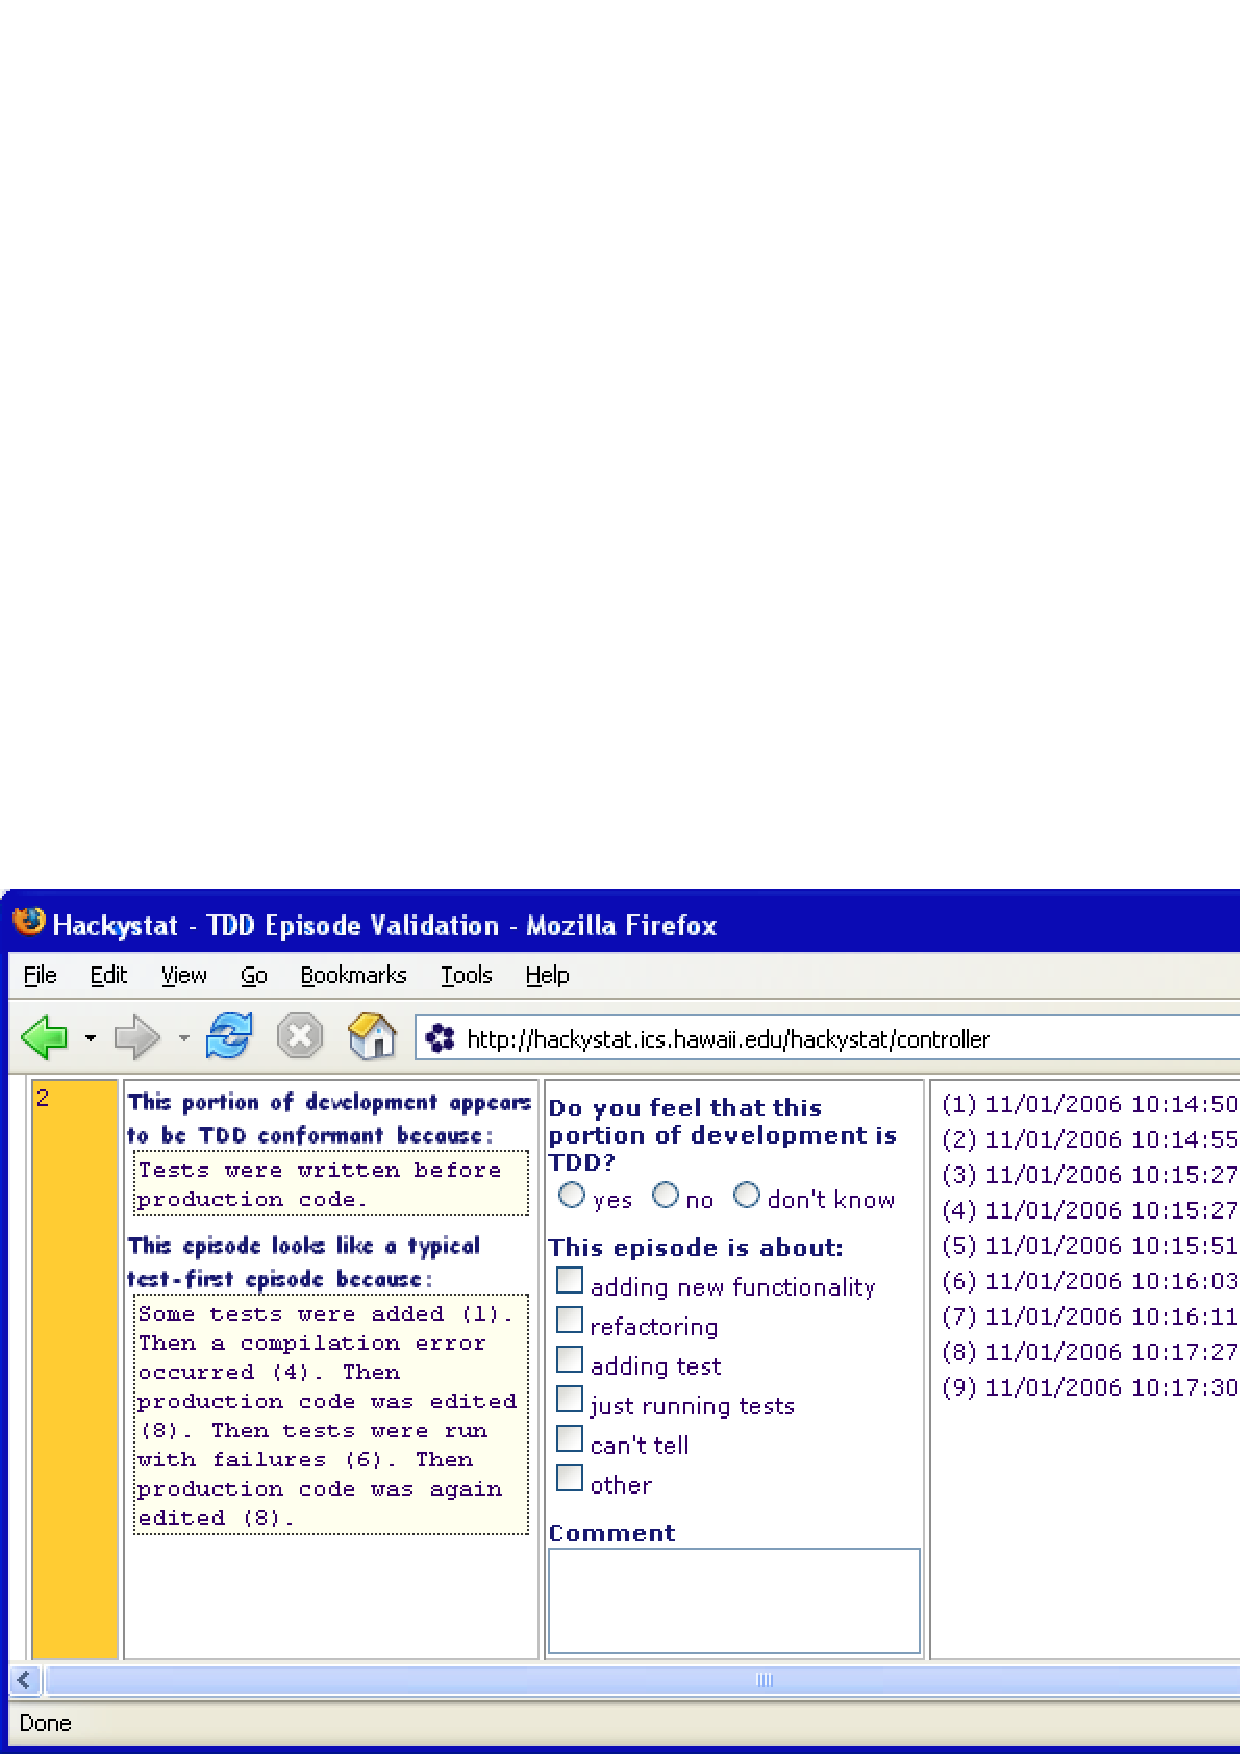
\includegraphics[width=1.0\textwidth]{figs/EpisodeFeedback}
  \caption{TDD Episode Validation}\label{fig:EpisodeFeedback}
\end{figure}
In addition to presenting inference results, this analysis also supplies Zorro's reasoning process and allows participants to give feedback, which was saved to the Hackystat server. Participants conducted Zorro usefulness evaluation using the ``Evaluation Wizard'' analysis (Figure \ref{fig:EvaluationWizard}) that saved the evaluation results to the Hackystat server too. 

%an episode validation analysis for users. This analysis presents Zorro's TDD behavior inference and the underlying reasoning process. It provides three choices for participants to indicate whether they agree or not with Zorro's inference on their TDD development behaviors. In the same analysis, they can also use a set of check-boxes and a text-box to provide additional information about their actual  development behaviors (Figure \ref{fig:EpisodeFeedback}).

%Hackystat sensor data and the participants' Zorro evaluations will  be stored at the remote Hackystat server. ESR will record the TDD  development process into QuickTime movie files in the lab computers. In the interview I will use notepad and tape recorder to record  the conversations with participants.

%\subsubsection{Participant Comment}
%TDD is a new practice aiming at ``clean code that works''. Red/green/refactor is Beck's simple model of TDD; however, it may be too simple for real world situations. For example, experienced TDD developers often write a series of tests that do not require additional production code implementation. In Zorro, I developed a set of rules to infer developer's TDD behavior based on Beck's TDD principle and additional knowledge from TDD practitioners. Therefore, Zorro's TDD inference is somewhat subjective.  The purpose of this analysis is to provide additional data from participants to cross-validate Zorro's TDD behavior inference. This effort supplies  research question Q2-4, that is, whether participants agree with Zorro's TDD developer behavior inference.

\section{Threats to Validty}
\label{sec:Classroom-Validity}
A construct validity problem existed in the pilot study. I, the author of Zorro, compared the recorded movies with Zorro's inference to validate Zorro's metrics collection and TDD development behavioral inference. I could be biased both at judging what software metrics are necessary, as well as at inferring development behaviors from the observed activities in the recorded movies. One person's subjective judgment, especially the one from the author, perhaps is not a valid measure in case studies \cite{Yin:03}. Therefore, I employed the additional evidence of participant comments to improve the construct validity. The participant comments were analyzed to cross-validate my video analysis. Compared to the pilot study, this additional source of evidence helped to solidify research conclusions, but note that a caveat did exist because the student participants could have given feedback that favored Zorro's behavioral inference.

It is challenging to validate Zorro because participants might not want to be instrumented by the sensors, not to mention having their development processes recorded with ESR. In my study, I used two lab PCs and carefully stated that participants were not evaluated based upon their performances, and they gained extra credit as long as they participated in this study. Moreover, participants' identities were not disclosed in any written documents. The consent form I used is available at the Appendix \ref{app:CaseStudyConsentForm}.

In term of external validity, only 11 students participated in this study. The sample size is small, which makes it difficult for me to generalize these research findings. Also, students in the software engineering classes at the University of Hawaii might not be representative of all TDD beginners since professional developers can also be TDD beginners. To improve external validity, replication studies need to be conducted in other organizations. For this purpose, I made all my research materials available to public.

%In order to generalize Zorro's TDD episode inference accuracy regarding hypothesis 2, we estimate sample size requirement according to \cite{Cochran:77}. The analysis unit is episode, and we select confidence level 95\%. To be statistically important, we will need 138~245 episodes. Since we may have 12 participants in this study, it will be enough if every participant contributes 20 or more TDD development episodes. A recent dry-run test revealed that one test subject can yield 23 episodes.

\section{Data Analysis Methods for An Individual Participant}
\label{sec:ClassroomAnalysisMethods}

%Each participant in this study developed a solution to the Bowling Score Keeper problem (Appendix \ref{app:UserStoriesBSK}) in the Eclipse IDE with the instrumentations using the Hackystat Eclipse Sensor and ESR. I collected both the participant's in-process development activities and the participant's development video. 

%During the data analysis process, I played ESR videos to observe participants' development activities and TDD development behaviors. Then I compared my observational results to data that was automatically collected and inferred by Zorro. Finally, I used the participants' comments as the second source of evidence for cross-validation.

%After the participant finished the programming task, I interviewed him/her on unit testing and TDD. Then the participant evaluated Zorro's usefulness. Thus, I had both the interview script and the participant's evaluation of Zorro. I analyzed these two types of data to investigate how useful Zorro is and how Zorro's analyses can be used in the teaching and practices of Test-Driven Development.

I processed every participant's data and drew research conclusions by putting analysis results of all participants together. This section introduces the analysis methods for an individual participant using the first participant's data. 

%After analyzing all participants' data, I summarized research results in next section (Section \ref{sec:CaseStudyFindings}). 

\subsection{Participant Observation and Validation of Data Collection}
\label{subsec:DevelopmentActivityObservation}

The first step was to observe the first participant by playing his development video recorded by ESR. This observation helped to validate Zorro's software metrics collection for him. 

\subsubsection {Analysis Method}
Similarly to the pilot study, I observed low-level development activities by playing the recorded ESR video from the first participant. Then I logged what I observed into an Excel spreadsheet for bookkeeping (See Figure \ref{fig:VideoExcelScript} in Chapter \ref{ch:Pilot}). Recall that SDSA constructs the development stream using software metrics collected by sensors (Section \ref{sec:SDSA-Construction}), so we can also construct another development stream using development activities that occurred in the participant's development process and that I observed in the recorded development video. To validate Zorro's data collection, I simply compared two development streams that were illustrated in Figure \ref{fig:DataVerification} in Chapter \ref{ch:Pilot}.  

%Thus I divided the development stream into episodes using successful unit test invocations in the end after finishing participant observation.

\subsubsection{Analysis Result}
The first participant finished 7 of the 13 user stories in 90 minutes. I observed that he conducted 153 development activities, which were then divided into 10 episodes. For each episode, Table \ref{tab:ActivityNumber} lists both the number of activities collected by Zorro and the number of activities I observed. The difference between the two numbers is in the ``Difference'' column. Descriptive analysis results are available at the bottom of this table.
\begin{table}[htbp]
\centering
  \caption{Number of Development Activities}\label{tab:ActivityNumber}  
  \begin{tabular}{|l|l|l|l|}
  \hline
    Episode &  Activities (Zorro)& Activities (Video) & Difference \\ \hline
    1	      &   4 &   4  &   0   \\ \hline
    2	      &   6 &   5  &  +1   \\ \hline
    3       &  13 &  11  &  +2   \\ \hline
    4       &  19 &  15  &  +4   \\ \hline
    5       &  23 &  19  &  +4   \\ \hline
    6       &  14 &   9  &  +5   \\ \hline
    7       &  46 &  35  &  +11  \\ \hline
    8       &  22 &  15  &  +7   \\ \hline
    9       &   5 &   5  &   0   \\ \hline
    10      &  46 &  35  &  +11  \\ \hline \hline
    Total   & 198 & 153  &       \\ \hline
    Mean    &     &      &  4.5  \\ \hline
    Median  &     &      &  4    \\ \hline
    STDEV   &     &      &  4.1  \\ \hline
    \end{tabular}
\end{table}

Note that ESR captures the Eclipse window once per second, so it should capture almost everything that happens in a programming session. However, according to Table \ref{tab:ActivityNumber}, activities collected by Zorro outnumbered activities I observed in the recorded video of the same development process conducted by the first participant. Moreover, the differences in activity numbers were significant according to the descriptive analysis. Zorro collected 19.8 activities per episode, which were 4.5 more than the number of activities per episode I observed in the video. 

\begin{comment}
Zorro collected 4.5 more activities per episode than I observed in the video on average. The standard deviation is 
\begin{equation} \label{StandardDeviation}
  s = \sqrt{\frac{\sum_{i=1}^{10}{(x_{i}-\bar{x})^2}}{n-1}} = 4.1.
\end{equation},
where \begin{math}s\end{math} standards for standard deviation, 
\begin{math}x_{i}\end{math} standards for the activity number difference 
of the \begin{math}ith\end{math} episode, and \begin{math}\bar{x}\end{math} 
is the mean of episode activity differences.
\end{comment}

\subsection{Validation of TDD Behaviors and TDD Compliance Inference}
\label{subsec:BehaviorComplianceValidation}

The second step was to validate Zorro's inference of TDD development behaviors and TDD compliance. 

\subsubsection{Analysis Method}
In Section \ref{subsec:DevelopmentActivityObservation}, I introduced how I observed development activities in the recorded video. In this step, I played the video again to observe TDD development behaviors of the first participant. Following this observation, I analyzed the TDD compliance of each episode. Similarly to what I did in Section \ref{subsec:DevelopmentActivityObservation}, I validated Zorro's inference results of TDD behaviors and TDD compliance by comparing what Zorro inferred to what I observed.

%While playing a participant's ESR video to observe his/her development activities, I also analyzed his/her TDD development behaviors. This technique is a variation of the participant observation for validating Zorro's automated TDD behavior inference machinery.

\subsubsection{Analysis Result}
I list the analysis result in Table \ref{tab:BehaviorObservation} in which Zorro's inference results are on the left and my observation analysis results are on the right. Recall that Zorro infers development behaviors in episodes first, and then infers TDD compliance based upon development context using heuristic algorithms (Section \ref{sec:Zorro-TDDConformance}). Therefore, I present Zorro's inference results in two columns in Table \ref{tab:BehaviorObservation}: one is for TDD development behaviors and the other one is for TDD compliance. In order to compare Zorro's inference results to my observation results, I also list the observation results in two columns: one is for development behaviors and the other one is for TDD compliance. 
\begin{table}[htbp]
\centering
  \caption{Comparison between Zorro Inference and Video Observation}  \begin{tabular}{|l|p{2cm}|l|p{2cm}|l|}
  \hline
         & \multicolumn{2}{c|}{Zorro} & 
           \multicolumn{2}{c|}{Observation} \\ \cline{2-5}
   \raisebox{1.5ex}[0pt]{Index} 
         & Behavior       & Is TDD? & Behavior      & Is TDD? \\ \hline
    1    & test-addition  & Yes	    & test-addition & Yes   \\ \hline
    2    & refactoring	  & Yes	    & refactoring   & Yes   \\ \hline
    3    & refactoring	  & Yes	    & refactoring   & Yes   \\ \hline
    4    & test-first     & Yes     & test-first    & Yes   \\ \hline
    5    & test-first     & Yes     & test-first    & Yes   \\ \hline
    6    & test-first     & Yes	    & test-first    & Yes  \\ \hline
    7    & test-first     & Yes	    & test-first    & Yes  \\ \hline
    8    & test-first     & Yes     & test-first    & Yes   \\ \hline
    9    & test-addition  & Yes	    & test-addition	& Yes	 \\ \hline
   10    & unknown        & No      & test-first    & Yes  \\ \hline 
  \end{tabular}
\label{tab:BehaviorObservation}  
\end{table}

From Table \ref{tab:BehaviorObservation}, we can see that participant observation results are identical to Zorro's inference results except for the last episode. Due to the 90-minute time constraint, the first participant did not finish the last user story he worked on. Thus the last episode did not end with any successful unit test invocation, which prevented Zorro from inferring the development behavior in it. In Chapter \ref{ch:Zorro}, we introduced that Zorro classifies an episode as ``Unknown'' if it does not end with a successful unit test invocation. This is often the situation at the end of a programming session.

\begin{comment}
Because the last episode was 
incomplete, Zorro did not recognize what happened in it. Other than this, 
the results inferred by Zorro and the results observed by me are
identical.

The data in Table \ref{tab:BehaviorObservation} provide complementary
evidence to the research finding in Section
\ref{subsec:DevelopmentActivityObservation} for the research question
Q2a. All episodes were partitioned and the development behaviors in
them were inferred correctly by Zorro if the last episode was not
considered.
\end{comment}

\subsection{Cross-validation of TDD Behaviors and TDD Compliance Inference}
\label{subsec:ParticipantValidation}
As the author of Zorro, my observation of development behaviors could be biased (Section \ref{sec:Classroom-Validity}). This bias would decrease construct validity \cite{Yin:03} if participant observation were the only data analysis method. To improve construct validity, I used an additional source of data -- participants' validation comments that were acquired through the ``TDD Episode Validation'' analysis (Section \ref{sec:Classroom-DataCollection}). 

\subsubsection{Analysis Method}
Similarly to the participant observation analysis in the previous step, I compared the first participant's validation comments episode by episode to Zorro's inference results for cross-validation. 

%The participant commented on his/her TDD development behaviors by answering the question -- ``Do you feel that this portion of development is TDD?''  and checking the following items that could be applied: ``adding new functionality'', ``refactoring'', ``adding test'', ``just running tests'', ``can't tell'' and ``other''. For the data analysis, I compared the participant's comments to Zorro's inferences to investigate how accurately Zorro can infer TDD behaviors in his/her opinion.

\subsubsection{Analysis Result}
In Table \ref{tab:ParticipantTDDBehavior}, I listed the first participant's comments along with both Zorro's inference and my video observation results. Note that the participant's comments on development behaviors are different from what Zorro inferred and what I observed in the ESR video because participants described their development behaviors by selecting them from the following list: 
\begin{itemize}
\item adding new functionality,
\item refactoring,
\item adding test,
\item just running tests,
\item can't tell,
\item other
\end{itemize}
for each episode. Because of this, it is impossible to directly compare what the participant agreed upon to be his development behaviors to what Zorro inferred and what I observed. Thus, I will introduce a mapping schema to make them comparable in Section \ref{sec:CaseStudyFindings} after processing all participants' data.

%Both Zorro and my video observation categorized the development behavior in each episode using the tacit knowledge of the TDD development patterns.

\begin{sidewaystable}[htbp]
\centering
  \begin{tabular}{|l|p{2cm}|l|p{2cm}|l|p{7.5cm}|l|}
  \hline
      & \multicolumn{2}{c|}{Zorro Inference} & \multicolumn{2}{c|}{Video Observation} & 
        \multicolumn{2}{c|}{Participant Comment} \\ \cline{2-7}
   \raisebox{1.5ex}[0pt]{Index} &
    Behavior      & Is TDD? & Behavior  & Is TDD? & Behavior & Is TDD? \\ \hline
1 & test-addition & Yes & test-addition & Yes & adding test  & Yes \\ \hline
2 & refactoring   & Yes & test-first    & Yes & refactoring & Yes  \\ \hline
3 & refactoring   & Yes & refactoring   & Yes & refactoring & Yes  \\ \hline
4 & test-first    & Yes & test-first    & Yes & adding new functionality, adding test & Yes	\\ \hline
5 & test-first    & Yes & test-first    & Yes & refactoring & Yes  \\ \hline
6 & test-first    & Yes & test-first    & Yes & adding new functionality, adding test & Yes \\ \hline
7 & test-first    & Yes & test-first    & Yes & adding new functionality, refactoring, adding test & Yes \\ \hline
8 & test-first    & Yes & test-first    & Yes & adding new functionality, adding test & Yes	\\ \hline
9 & test-addition & Yes & test-addition & Yes & adding test & Yes  \\ \hline
10 & unknown      & No  & test-first    & Yes & adding new functionality, refactoring, adding test & Yes \\ \hline 
  \end{tabular}
  \caption{Participants' Comments on their Development Behaviors}
  \label{tab:ParticipantTDDBehavior}  
\end{sidewaystable}

In term of TDD compliance, the first participant believed that his development process was 100\% TDD compliant, which is slightly different from what Zorro inferred but conformant to what I observed in the video. As I discusssed in Section \ref{subsec:BehaviorComplianceValidation}, this difference is caused by Zorro's stringent requirement that an episode must end with successful unit test invocations. 

\begin{comment}
Although the terms for describing episode behaviors were different,
the participant's comments provided enough information to validate
Zorro's episode behavior inference. For example, the first participant
agreed that Zorro correctly inferred the behaviors in episodes 1, 2,
3, and 9. Episodes 4, 6, 7, and 9 are ``test-driven'' with compound
development behaviors from the participant's points of view. 

Most importantly, the participant's comments provided the additional
information to cross-validate the video analysis method. For the first
participant, his comments were very close to what I have observed
using the video analysis. 
\end{comment}

\subsection{Participant Interview Analysis using the Coding Method}
\label{subsec:InterviewAnalysis}

%The red/green/refactor metaphor is a simple and abbreviated abstraction of TDD. A developer may conduct TDD development differently depending upon his/her programming experiences and understandings of TDD. Sometimes a developer may choose to violate the principles of TDD intentionally. In this study, I interviewed the participant on unit testing and TDD. 

I analyzed the first participant's interview data to study his opinions on unit testing and TDD using the coding analysis method.

\subsubsection{Analysis Method}
Coding is a data analysis method that can generate a description of setting or people as well as categories or themes\cite{Creswell:03,GroundedTheory}. For interview conducted in this study, I coded participants into different categories according to their opinions on software development, unit testing, and TDD. 

\subsubsection{Analysis Result}

Table \ref{tab:InterviewQuestionAndAnswer} summarizes the interview questions and answers from the first participant.

\begin{table}[htbp]
\centering
  \caption{List of Interview Questions and Answers}
  \begin{tabular}{|l|p{8cm}|}
  \hline
    Interview Question & Participant's Response \\ \hline
    Unit testing experience         & Several years.\\ \hline
    Prior unit testing strategy     & Write test after production iteratively.\\ \hline
    How much unit testing           & Not all the time. \\ \hline
    TDD's impact on unit testing    & TDD is messy and leads to wrong design. 
                                      TDD is better if there is good design first. \\ \hline
    Comfortableness of TDD          & Hard, especially when a refactoring activity  
                                      caused previous tests failed (regression test failure). 
                                      \\ \hline
    Full-scale use of TDD           & Do not want to do so until I get accustomed 
                                      to it. Likes the idea of TDD.\\ \hline
  \end{tabular}
  \label{tab:InterviewQuestionAndAnswer}  
\end{table}

In the interview, the first participant stated that unit testing was a practice that was required in his prior software development. In his opinion, iteratively implementing test cases afterward makes more sense than writing test first.  Additionally, TDD may lead to wrong design and messy code if there is no good design first. Therefore, implementing software in TDD is hard and it takes time to get accustomed to it. With these answers, I coded a category named``somewhat in favor of unit testing but not in favor of TDD''. 

%Moreover, his answers reflected what had happened in the last episode, in  which the revised production code failed some regression tests and he could not make all tests pass at the end. 

\subsection{Reporting Usefulness of Zorro's Analyses}
\label{subsec:UsefulnessEvaluation}

With the navigation of the ``Zorro Evaluation Wizard'', participants conducted five Zorro's analyses on their own TDD development conducted in this study. After reviewing each analysis, they evaluated its usefulness. I generated the usefulness evaluation results in this step.

\subsubsection{Analysis Method}

%While evaluating Zorro's usefulness, the first participant also expressed how strongly he agreed that Zorro's analyses were useful. 
The evaluation of usefulness varies from ``Strongly Disagree'' to ``Strongly Agree'', which are quantified into values from 1 to 5 (Table \ref{tab:UsefulnessScale}).
\begin{table}[htbp]
\centering
  \caption{Table of Usefulness Scale}\label{tab:UsefulnessScale}  
  \begin{tabular}{|l|l|}
  \hline
   Strengthen        & Scale \\ \hline
   Strongly Disagree & 1 \\ \hline
   Disagree          & 2 \\ \hline
   Neutral           & 3 \\ \hline
   Agree             & 4 \\ \hline
   Strongly Agree    & 5 \\ \hline
  \end{tabular}
\end{table}
In addition to the scale of usefulness, participants also checked areas that were helpful after reviewing each analysis. Table \ref{tab:UsefulAreas} lists all possible useful areas that are encoded to UA-1, UA-2, and UA-3 etc.
\begin{table}[htbp]
  \centering
  \caption{Table of Useful Areas}\label{tab:UsefulAreas}  
  \begin{tabular}{|l|l|}
  \hline
  Code & Useful Area \\ \hline
  UA-1 & Acquiring awareness of my programming patterns \\ \hline
  UA-2 & Learning TDD \\ \hline
  UA-3 & Mastering TDD \\ \hline
  UA-4 & Monitoring my pace \\ \hline
  UA-5 & Improving my programming skills \\ \hline
  UA-6 & Discovering the situations in which TDD is useful \\ \hline
  UA-7 & Discovering the situations in which TDD is applicable \\ \hline
  UA-8 & Gauging how much testing I am doing \\ \hline
  UA-9 & Other \\ \hline
  \end{tabular}
\end{table}

\subsubsection{Analysis Result}

Table \ref{tab:FirstUsefulness} is a summary of the first participant's evaluation on Zorro's usefulness. Note that he only evaluated 4 of 5 analyses because the ``Effort T/P Ratio'' analysis had a bug at that time, which was fixed after he finished participating in this study.
\begin{table}[!ht]
\centering
  \caption{The First Participant's Usefulness Evaluation}\label{tab:FirstUsefulness}
  \begin{tabular}{|l|l|l|l|l|l|l|l|l|l|l|}
  \hline
           &      & \multicolumn{9}{c|}{Areas} \\ \cline{3-11}
    \raisebox{1.5ex}[0pt]{Analysis Name}   & \raisebox{1.5ex}[0pt]{Scale} 
       & UA-1 & UA-2 & UA-3 & UA-4 & UA-5 & UA-6 & UA-7 & UA-8 & UA-9   \\ \hline
    Demography Analysis & 3   &   & X &   &   & X &   & X &   &   \\ \hline       
    Effort T/P Ratio    & N/A &   &   &   &   &   &   &   &   &   \\ \hline
    Size T/P Ratio      & 2   &   &   &   & X &   &   &   &   &   \\ \hline
    Duration            & 3   &   &   &   & X &   &   &   &   &   \\ \hline
    Duration Histogram  & 2   &   &   &   & X &   &   &   &   &   \\ \hline
  \end{tabular}
\end{table}

The first participant thought that Zorro's analyses were somewhat useful to him. According to his evaluation, the ``TDD Episode Demography'' analysis was most useful for learning TDD whereas other analyses were only good at showing his development pace. 

\section{Classroom Study Data Analysis Results}
\label{sec:CaseStudyFindings}

In the data analysis, I assigned letters `A', `K', `L', `M', `N', `O', `P', `Q', `R', `S', and `T' to 11 participants as their identifications. Using the data analysis methods introduced in the previous section (Section \ref{sec:ClassroomAnalysisMethods}), I analyzed data collected from all participants and presented results in the following.  

\subsection{An unexpected phenomenon and participant grouping}
\label{subsec:ParticipantGroup}
%, which impacted Zorro's development stream partition and TDD behavior inference. 
First, I will introduce an unexpected phenomenon I discovered in the data analysis. In Chapter \ref{ch:RelatedWork}, we have discussed that TDD is iterative and incremental. The rhythm of TDD is\cite{Beck:03}:
\begin{enumerate}
  \item Quickly add a test.
  \item Run all the tests and see the new one fail.
  \item Make a little change.
  \item Run all tests and see them all succeed.
  \item Refactor to remove duplication.
\end{enumerate}

%Through literature readings, my personal practices, and observation of others programming in TDD, this partition technique should work very well toward recognizing the TDD practices.
Based upon the rhythm of TDD, I designed Zorro to partition a TDD development stream over a time period into episodes using successful test invocations as tokens (Chapter \ref{ch:Zorro}). Also in Chapter \ref{ch:Zorro}, I have shown that the ``Test-Pass'' tokenizer is sufficient for identifying TDD iterations. However, in this study, I found an unexpected phenomenon that made the partitioning of several episodes problematic. The cause is that in the step 2 of the TDD rhythm, ``run all the tests and see the new one fail'' does not occur as expected when compilation errors exist. Although Eclipse, the IDE I used in this study, prompted a warning message in this case and allowed developers to cancel test invocations, some developers opted not to. As a result, sometimes test invocations succeeded unexpectedly regardless of compilation errors. In consequence, Zorro failed to partition some episodes, which led to development stream partitioning and behavioral inference errors.

To investigate how this phenomenon affected Zorro, I divided participants into groups G1 and G2 based upon their test invocation behaviors.
\begin{itemize}
\item \textbf{G1} Participants who canceled a test invocation when compilation error(s) existed.
\item \textbf{G2} Participants who continued a test invocation regardless of the existence of compilation error(s).
\end{itemize}
Among 11 participants, 4 of them are in group G1 and 7 of them are in group G2 (see Table \ref{tab:ParticipantCategory}).  
\begin{table}[!ht]
\centering
  \caption{Participant Groups}\label{tab:ParticipantCategory}  
  \begin{tabular}{|l|l|l|l|}
  \hline
    Group &  Participants \\ \hline
    G1:	     &  K, L, O, and R \\ \hline
    G2:	     &  A, M, N, P, Q, S, and T  \\ \hline
    \end{tabular}
\end{table}
Because development stream partitioning and behavioral inference errors only occurred to participants in group G2, I will term this phenomenon as G2-DevBehavior in the rest of this document. I will also discuss how Zorro can be improved if we can avoid this problem.

\subsection{Validation of Data Collection}
\label{subsec:SensorDataValidation}
Using the participant observation research method discussed in Section \ref{subsec:DevelopmentActivityObservation},  I validated Zorro's data collection for all participants. 

\subsubsection{Analysis Result}
Table \ref{tab:ActivityNumberSummary} presents numbers of development activities for each participant. The first column includes participant IDs. The second column has numbers of episodes that were partitioned by Zorro. For each participant, I listed his/her development activities per episode in columns 3 and 4. The number of activities collected by Zorro is in column 3 and the number of activities I observed is in column 4. The rest two columns have mean and median values of episode activity number differences.

\begin{table}[!ht]
\centering
  \caption{Summary of Development Activities}\label{tab:ActivityNumberSummary} 
  \begin{tabular}{|l|r|r|r|r|r|}
  \hline
    &  &  \multicolumn{2}{c|}{Activities per Episode} & 
          \multicolumn{2}{c|}{Activity Difference} \\ \cline{3-6}
    \raisebox{1.5ex}[0pt]{ID} & \raisebox{1.5ex}[0pt]{Episodes}  & 
                 Zorro & Video Observation & Mean & Median \\ \hline
         A  & 19   & 12.7 & 11.9 & 0.8 & 0   \\ \hline  
         K  & 10   & 19.8 & 15.3 & 4.5 & 4   \\ \hline
         L  &  8   & 32.5 & 30.4 & 2.1 & 2   \\ \hline  
         N  &  9   & 20.4 & 18.2 & 2.2 & 3   \\ \hline
         O  & 16   & 15.3 & 13.6 & 1.7 & 0.5 \\ \hline
         P  & 18   & 13.7 & 11.7 & 2.1 & 1.5 \\ \hline
         Q  & 21   &  9.8 &  9.6 & 0.5 & 0   \\ \hline
         R  & 14   & 12.6 & 11.2 & 1.4 & 0   \\ \hline
         S  &  9   & 16.3 & 12.7 & 3.7 & 2   \\ \hline
         T  & 13   & 15.3 & 13.2 & 2.1 & 1   \\ \hline
       Mean & 13.8 & 16.8 & 14.8 & 2.1 & 1.4 \\ \hline 
    \end{tabular}
\end{table}

Note that I excluded data from participant `M' in Table \ref{tab:ActivityNumberSummary} that helped me find a bug in the Eclipse sensor. The bug was caused by the G2-DevBehavior I discussed in the previous section (Section \ref{subsec:ParticipantGroup}). At the time when G2-DevBehavior occurred, a run time exception was thrown but the Eclipse sensor did not handle it gracefully such that some development activities from participant `M' were missing. Though I improved the Eclipse sensor after finding this bug, some data from participant `M' were permanently lost. So in the rest of this document, I will not include his data, which reduced the number of effective participants to 10.

\subsubsection{Discussion}
According to analysis results presented in Table \ref{tab:ActivityNumberSummary}, Zorro is capable of collecting development activities. On average, Zorro collected more development activities (16.8 per episode) than what I observed (14.8 per episode). Both the mean and median values of episode activity number differences are positive.

In addition to computing differences of development activities, I also did further investigation to find what caused them by comparing development activities collected by Zorro to development activities I observed. 
\begin{figure}[htbp]
  \centering
  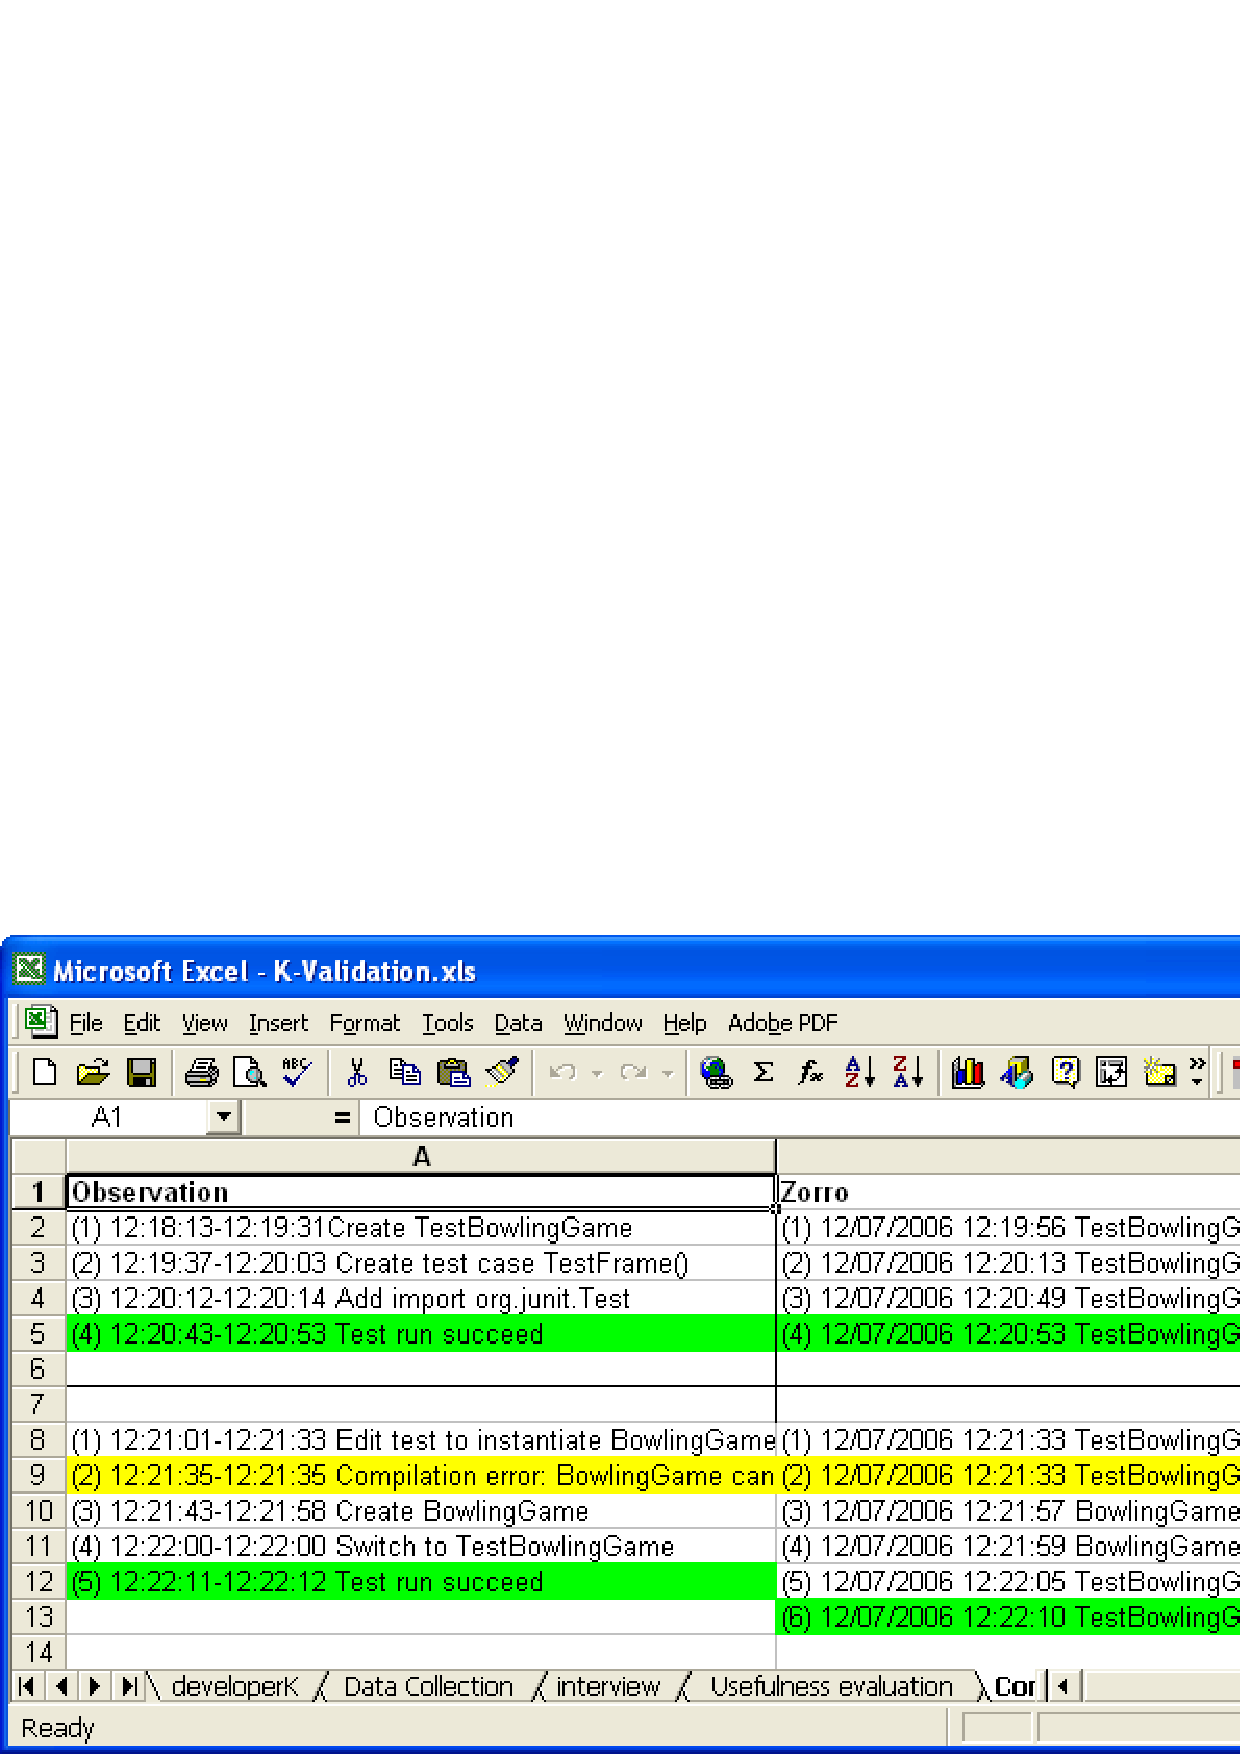
\includegraphics[width=1.0\textwidth]{figs/ZorroSensorDataValidation}
  \caption{Validation of Zorro's Development Activities}
  \label{fig:ZorroDataValidation}
\end{figure}

With side by side comparison (Figure \ref{fig:ZorroDataValidation}), I found two categories of situations that were responsible for Zorro's excessive data collection in the following. First, Zorro sometimes reported two or more activities while I only observed one development activity as what I described in the item of ``Kill two birds with one stone''. Second, though technically ESR should capture everything that happens in the Eclipse IDE, it did not in situations that were described in items of ``Invisible editing activities'' and ``Problems view of Eclipse could be hidden''. %Nearly 100\% of development behaviors I observed in ESR videos could be found in Zorro, but the relationship was not always one-to-one. Sometimes Zorro 

\begin{enumerate}
\item Kill two birds with one stone
  
When a developer changed statements that were associated with object components such as import, package declaration, attributes, method name, method return type, or method parameters, the Eclipse sensor collected two types of development activities: editing and refactoring. Similarly the Eclipse sensor would also collect both types of development activities when a developer used refactoring commands supplied in Eclipse. In both cases, Zorro doubled development activities. 

\item The problems view of Eclipse was hidden
  
In videos of participants `K', `M', and `T', the problems view of Eclipse was overlapped by other views for a while (see Figure \ref{fig:InvisibleEclipseProblemView}). I cannot observe compilation errors in this situation because Eclipse reports them in the problems view.  For instance, in Figure \ref{fig:InvisibleEclipseProblemView}, the JavaDoc view overlapped the problems view.  Since the title of the problems view was highlighted, it probably meant that there should have had compilation errors, but I could not tell it by watching the ESR video. 
  \begin{figure}[htbp]
    \centering
    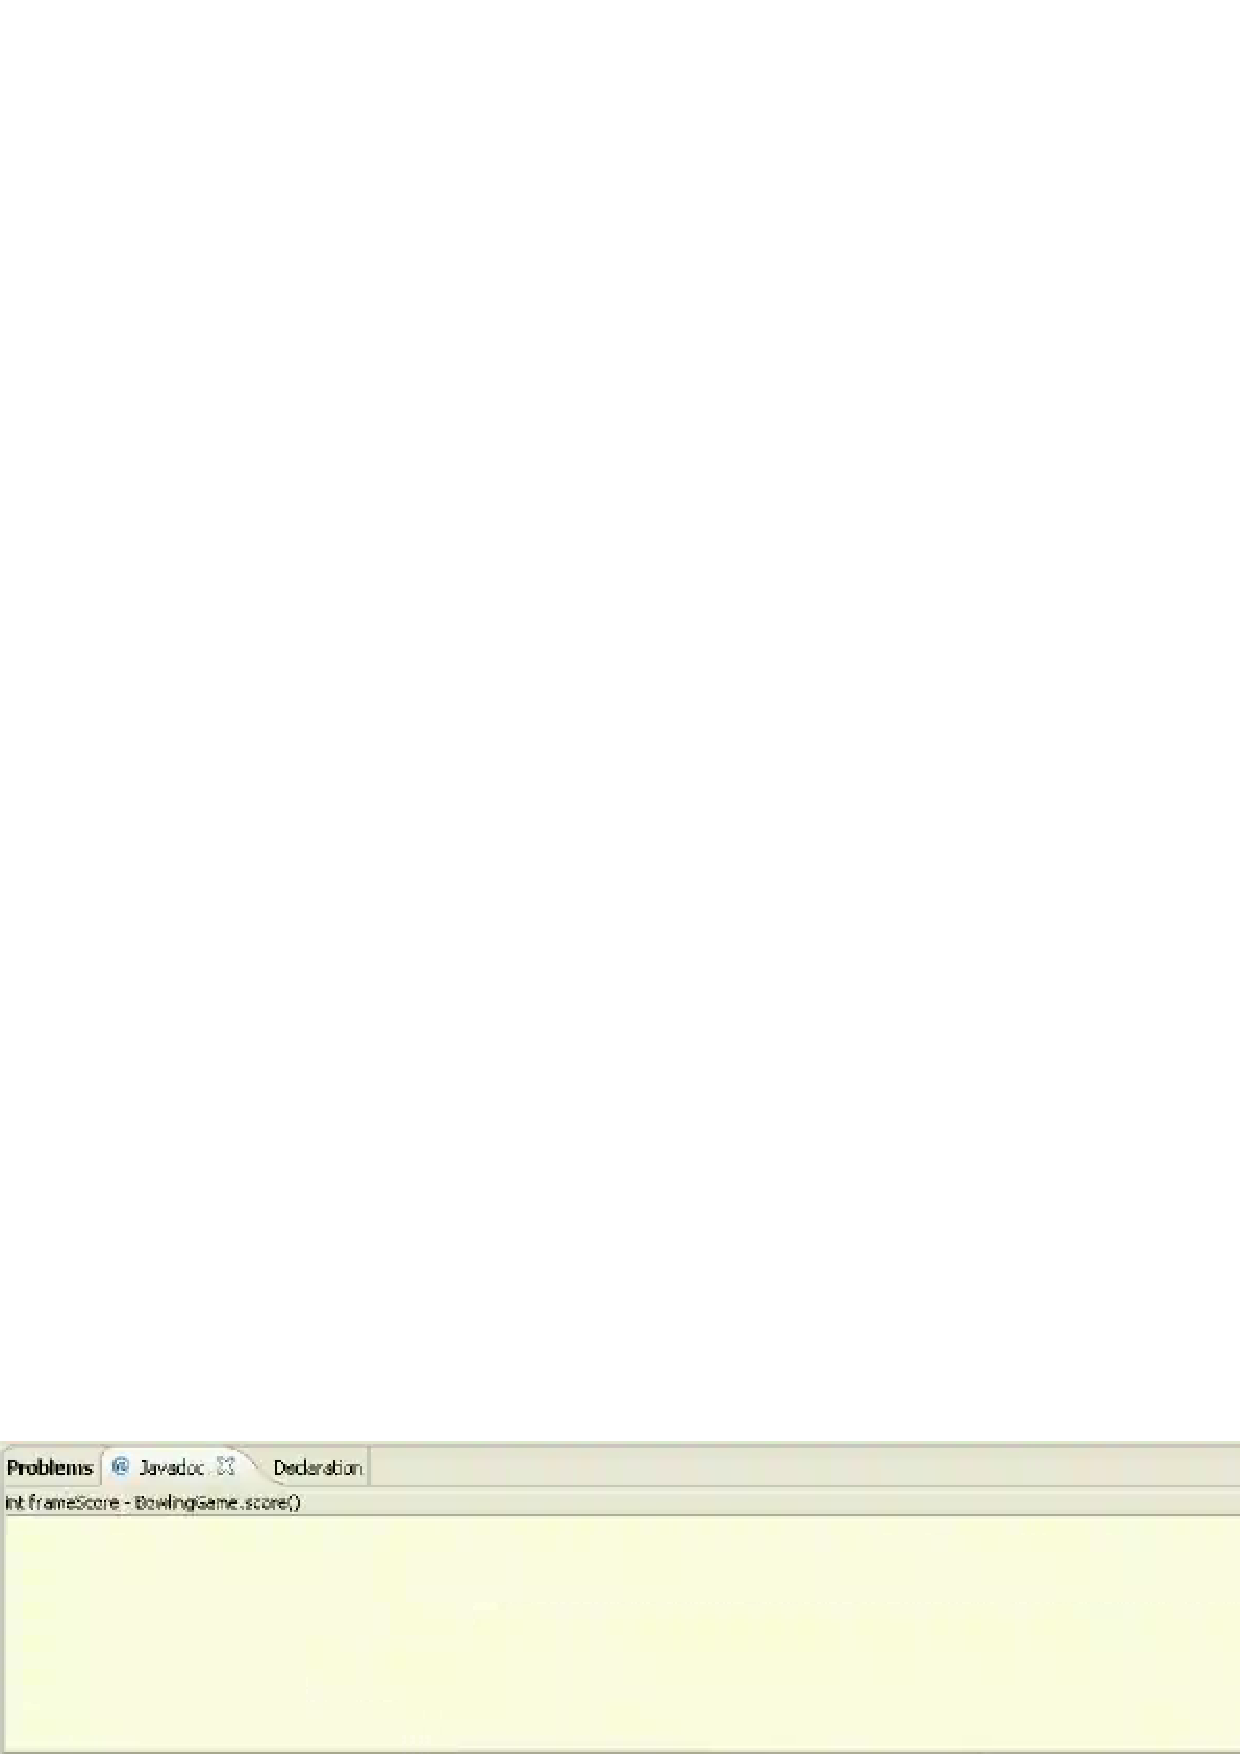
\includegraphics[width=0.8\textwidth]{figs/ESR-InvisibleProblemPane}
    \caption{Invisible Problems View in Eclipse}
    \label{fig:InvisibleEclipseProblemView}
  \end{figure}  

\item Invisible editing activities

A developer could input a few blank spaces while programming. Since ESR captured the screen of Eclipse, I would not be able to observe this kind of development activities because there is no visible changes. 

\end{enumerate}

The above three items can answer why Zorro collected more development activities than what I observed in recorded videos. However, there were also a few cases in which Zorro missed development activities (see items ``Quick editing'' and ``Quick buffer transition'').
\begin{enumerate}
 
\item Quick editing

The Eclipse sensor uses ``state change'' as the foundation to detect editing development activities. A timer thread in the sensor wakes up every 10 seconds to check the active buffer. If there are any changes made to the active buffer, the sensor will fire a ``state change'' event. Zorro reduces a series of consecutive ``state change'' events into an editing activity when processing development streams. This mechanism works well unless a developer edits a file for less than 10 seconds and then switches to another buffer. If so, the Eclipse sensor will miss an editing development activity.

\item Quick buffer transition
  
The Eclipse sensor collects ``buff trans'' activities by checking the active buffer.  A timer thread wakes up every 5 seconds to detect whether there is a buffer transition activity. Five-second is a small time period, but it is long enough for a developer to change the active buffers two or more times. If two or more consecutive buffer transition activities occur in less than 5 seconds, the Eclipse sensor might fail to capture some or all of them.
   
\end{enumerate}        

\subsubsection{Conclusion}
In this section, I summarized Zorro's data collection validation results (see Table \ref{tab:ActivityNumberSummary}). It turned out that Zorro collected more development activities per episode than I observed for every participant. Further investigation indicated that Zorro only missed a few development activities when participants quickly edited code or switched buffers. Also, Zorro collected development activities that were invisible in recorded videos. The analysis in this section indicates that there is partial supporting evidence for the research questions Q2a because Zorro can collect development activities more precisely than ESR, a recorder that can capture almost every development activity that occurs in the Eclipse IDE.  

\subsection{Validation of TDD Behaviors and TDD Compliance Inference}
\label{subsec:VideoObservationValidation}
Zorro recognizes TDD development through two steps (Chapter \ref{ch:Zorro}): (1) inferring development behaviors by matching development activities in episodes to a set of predefined development behaviors; (2) and then deducing TDD compliance using inferred episode behaviors. Thus, in this study, the validation analysis also had two steps: episode behavioral inference validation and TDD compliance inference validation, both of which were introduced in Section \ref{subsec:BehaviorComplianceValidation} for an individual participant. After validating Zorro for all participants, I summarized validation results in this section.

\subsubsection{Validation of Development Behavioral Inference}
\label{subsubsec:EpisodeBehavior}
For an individual participant I created a table similar as Table \ref{tab:BehaviorObservation} after validating Zorro's inference of his/her development behaviors. I then assigned the value 1 to an episode if the development behavior I observed in the video agrees with the development behavior Zorro inferred. In the end, I counted the number of 1's episodes and presented results in Table \ref{tab:EpisodeBehaviorAgreed} in which the last column is the percentage of 1's episodes to total episodes. This percentage could be an indicator of Zorro's development behavioral inference accuracy. 
\begin{table}[!ht]
\centering
  \caption{Video observation validation of development behaviors}
  \begin{tabular}{|l|r|r|r|}
  \hline
    ID & Episodes  & 1's Episodes & Percentage \\ \hline
    A       & 19   &  15   & 78.9\% \\ \hline  
    K       & 10   &   8   & 80.0\% \\ \hline
    L       &  8   &   7   & 87.5\% \\ \hline  
    N       &  9   &   4   & 44.4\% \\ \hline
    O       & 16   &  15   & 93.8\% \\ \hline
    P       & 18   &  12   & 66.7\% \\ \hline
    Q       & 21   &  11   & 52.4\% \\ \hline
    R       & 14   &  13   & 92.9\% \\ \hline
    S       &  9   &   2   & 22.2\% \\ \hline
    T       & 13   &   9   & 69.2\% \\ \hline
    Total   & 137  &  96   & 70.1\% \\ \hline
    \end{tabular}
  \label{tab:EpisodeBehaviorAgreed} 
\end{table}

In total, the participant observation analysis agreed that Zorro correctly inferred development behaviors in 96 episodes resulting in 70.1\% inference accuracy. But the inference accuracy is inconsistent from participant to participant. The lowest is 22.2\% and the highest is 93.8\% (Table \ref{tab:EpisodeBehaviorAgreed}). 

To address this inconsistency, one thing we can do is to study the impact of G2-DevBehavior by separating Table \ref{tab:EpisodeBehaviorAgreed} into two sub-tables: one for group G1 (Table \ref{tab:EpisodeBehaviorAgreedG1}), and the other one for group G2 (Table \ref{tab:EpisodeBehaviorAgreedG2}). 
\begin{table}[!ht]
\centering
  \caption{Video observation validation of development behaviors for G1}
  \begin{tabular}{|l|r|r|r|}
  \hline
    ID & Episodes  & 1's Episodes & Percent \\ \hline
    K       & 10   &   8   &  80.0\%  \\ \hline
    L       &  8   &   7   &  87.5\%  \\ \hline  
    O       & 16   &  15   &  93.8\%  \\ \hline
    R       & 14   &  13   &  92.9\%  \\ \hline
    Total   & 48   &  43   &  89.6\%  \\ \hline
    \end{tabular}
  \label{tab:EpisodeBehaviorAgreedG1} 
\end{table}
\begin{table}[!ht]
\centering
  \caption{Video observation validation of development behaviors for G2}
  \begin{tabular}{|l|r|r|r|r|}
  \hline
    ID & Episodes  & 1's Episodes & Percent & Episodes with G2-DevBehavior\\ \hline
    A       & 19   &  15   &  78.9\%  & 3  \\ \hline  
    N       &  9   &   4   &  44.4\%  & 3  \\ \hline
    P       & 18   &  12   &  66.7\%  & 4  \\ \hline
    Q       & 21   &  11   &  52.4\%  & 9  \\ \hline
    S       &  9   &   2   &  22.2\%  & 2  \\ \hline
    T       & 13   &   9   &  69.2\%  & 3  \\ \hline
    Total   & 89   &  53   &  59.6\%  & 24 \\ \hline
    \end{tabular}
  \label{tab:EpisodeBehaviorAgreedG2} 
\end{table}
Clearly, Zorro performed much better on inferring development behaviors for group G1 than for group G2. For G1, the average inference accuracy was 89.6\%, which is much higher than the average accuracy for G2. It indicates that G2-DevBehavior, which affected 24 out of 89 episodes, had a substantial impact on the accuracy of Zorro's inference of development behaviors. 

%In the best case, Zorro inferred 78.9\% of episode behaviors correctly for group G2 participants; on the contrary, even the lowest inference accuracy for group G1 participants is already 80.0\%. Of 89 episodes in Table \ref{tab:EpisodeBehaviorAgreedG2}, 24 were affected by the G2-DevBehavior. So it had great impacts on Zorro's development stream partition and episode behavior inference.

\subsubsection{Validation of TDD Compliance Inference}
Table \ref{tab:BehaviorObservation} lists not only development behaviors I observed but also TDD compliance for an individual participant. An episode is TDD compliant if its development behavior is either a portion of a TDD iteration such as refactoring or a complete TDD iteration. After observing TDD compliance for all participants, I summarized results in Table \ref{tab:TDDCompliantEpisodeNumber} for validation. 

%Zorro partitions a participant's development stream into episodes and infers the TDD compliance of those episodes. An episode is TDD compliant if its development behavior is either a portion of a TDD iteration, such as refactoring, or a complete TDD iteration. Beyond validating episode behavior inference, I also validated Zorro's TDD compliance inference. Table \ref{tab:TDDCompliantEpisodeNumber} lists the validation results. In the ``TDD Compliant Episodes'' columns, I include the number of TDD compliant episodes inferred by Zorro, the number of TDD compliant episodes I observed in the videos, and the difference between them for each participant. 
\begin{table}[!ht]
\centering
  \caption{Video observation validation of TDD compliance}
  \begin{tabular}{|l|r|r|r|r|}
  \hline
    &  &  \multicolumn{3}{c|}{TDD Compliant Episodes} \\ \cline{3-5}
    \raisebox{1.5ex}[0pt]{ID} & \raisebox{1.5ex}[0pt]{Episodes}  & 
     By Zorro &  By Video Analysis & Difference\\ \hline
    A       &  19   &  10    &  12  & -2  \\ \hline  
    K       &  10   &   9    &  10  & -1  \\ \hline
    L       &   8   &   7    &   7  &  0  \\ \hline  
    N       &   9   &   6    &   8  & -2  \\ \hline
    O       &  16   &  15    &  16  & -1  \\ \hline
    P       &  18   &  16    &  18  & -2  \\ \hline
    Q       &  21   &  21    &  21  &  0  \\ \hline
    R       &  14   &  13    &  14  & -1  \\ \hline
    S       &   9   &   3    &   9  & -6  \\ \hline
    T       &  13   &  13    &  13  &  0  \\ \hline
    Total   & 137   & 113    & 128  & -15 \\ \hline
    Mean    &      &        & 	& -1.5 \\ \hline
    Median  &      &        & 	& -1  \\ \hline
    STDEV   &      &        & 	& 1.78 \\ \hline
    \end{tabular}
  \label{tab:TDDCompliantEpisodeNumber} 
\end{table}
In Table \ref{tab:TDDCompliantEpisodeNumber}, the ``TDD Compliant Episodes'' column has numbers of TDD compliant episodes. It is divided into three sub-columns: ``By Zorro'', ``By Video Analysis'' and ``Difference''. With values in Table \ref{tab:TDDCompliantEpisodeNumber}, we can compute percentages of TDD compliant episodes in the following:
\begin{eqnarray}
%\[
   TDD(Zorro)\% & = & \frac{CompliantEpisodes(Zorro)}{TotalEpisodes} * 100 \nonumber \\
                & = & \frac{113}{137} * 100 \nonumber \\
                & = & 82.5, \nonumber \\ 
                            \nonumber \\
%\]
%\[
   TDD(Video Analysis)\% & = & 
                     \frac{CompliantEpisodes(VideoAnalysis)}{TotalEpisodes} * 100 \nonumber \\
                         & = & \frac{128}{137} * 100 \nonumber \\
                         & = & 93.4. \nonumber 
%\]
\end{eqnarray}

Using episode numbers as the measurement, Zorro is somewhat conservative on inferring TDD compliance compared to the participant observation analysis. The latter found that participants in this study complied to TDD in 93.4\% of episodes, while Zorro inferred that 82.5\% of episodes were TDD compliant. In Table \ref{tab:TDDCompliantEpisodeNumber}, I computed the episode number difference for all participants. The mean value is -1.5 and the standard deviation is 1.78, both of which are very small. %Thus, the participant observation analysis validation provides supporting evidence to the research question Q2b: \textit{Does Zorro�s inference of TDD behaviors agree with analyses based upon participant observation?}

However, the above evidence was not sufficient because the sample size was too small. Eleven  students participated in this study and I can only analyze data collected from 10 of them. In order to generalize research conclusions, it is necessary to include more participants. But the resource was limited in this study since the two software engineering classes only had 16 students (Section \ref{sec:ClassroomDesign}). 

%Fortunately, this limitation can be improved using the bootstrap resampling technique \cite{Resampling}. 

\begin{comment}
Resampling has many types and one of them is bootstrapping that can be used to estimate the precision of sample statistics \cite{Resampling} such as confidence interval and distribution of the sample mean. Bootstrap sampling is to sample randomly with replacement from a set of data points. In Figure \ref{fig:Bootstrap}, Dr. Teknomo introduced it using five balls and a basket to illustrate how it works. 
\begin{figure}[htbp]
  \centering
  \includegraphics[width=0.4\textwidth]{figs/BootstrapSampling}
  \caption{Randomly Sampling with Replacement \cite{BootstrapTutorial}}
  \label{fig:Bootstrap}
\end{figure}
Suppose that a sample contains 5 observations. We label them with 5 balls named `A', 'B', 'C', 'D', and 'E', and then put them into the basket. We randomly draw one ball from the basket, record its name, and then put it back into the basket. This is sampling with replacement with which we can increase sample size even though the available sample size is small. 

With bootstrapping, I raised sample size from 10 to 200 and computed descriptive statistic values (Table \ref{tab:BootstrapTDDPercent}). Note that the significant level was 0.05 (alpha value). 
\begin{table}
  \centering
  \caption{Descriptive Analysis of TDD\% with Bootstrapping}
  \begin{tabular}{|l|l|l|} \hline
                &  TDD\% (Zorro) & TDD\% (Video Analysis) \\ \hline
    Mean        &  80.4          & 93.9    \\ \hline
    Median      &  88.9          & 100.0   \\ \hline
    STDEV       &  21.3          & 11.4    \\ \hline
    Lower Bound &  63.8          & 85.3    \\ \hline 
    Upper Bound &  94.8          & 100.0   \\ \hline
  \end{tabular}
  \label{tab:BootstrapTDDPercent}  
\end{table}
According to Zorro's inference, the mean of participants' TDD compliance was 80.4\%. It indicates that Zorro can infer the compliance to TDD when it happens. Since participants did not comply to TDD all the time (93.9\%), Zorro's TDD compliance inference accuracy should be higher than 80.4\%. However, the standard deviation 21.3 was a little high and the confidence interval is a little wide ([63.8\%, 94.8\%]). 
\end{comment}

Next, I will discuss whether and how G2-DevBehavior affected Zorro's TDD inference by separating participants into groups G1 and G2. 

%However, this judgment is a bit premature because the mean and standard devision are not sufficient. A convincing conclusion must be accompanied by much stronger statistics analyses. In the next paragraph I will briefly introduce the goodness-of-fit of model to data, a statistics analysis method plausible for evaluating the fitness of Zorro's inference results to my video analysis results.

\begin{comment}
Since there are two sets of data, a temptation is to apply a parameter statistics test such as the t-test and f-test, or a nonparameter statistics test such as the chi-square test \cite{GoodnessOfFit,Anderson:86}, but none of them is appropriate for testing the goodness-of-fit. Fundamentally, statistics tests are meant to find evidence that the difference between the two or more sets of data is not caused by chance. In term of validating how accurately Zorro infers TDD, we are looking for some measures that can indicate how well Zorro is doing. Sadly, there are no formal standards with regard to the goodness-of-fit analysis method according to \cite{Schunn:05}. As a result, there are various methods and they are often used  incorrectly. In \cite{Schunn:05}, Schuun and Wallach recommend a combination of $r^2$ and RMSD (root mean squared  deviation) or RMSSD (root mean squared scaled deviation). $r^2$ is the square of Pearson correlation coefficient $r$ \cite{Anderson:86}. It measures how well relative trend magnitudes are captured \cite{Schunn:05}. That is, how well Zorro's inference predicates the video analysis. Note that $0\leq r^2 \geq1$. If $ r^2=1 $, Zorro's inference of TDD fits the video analysis perfectly. The $r^2$ alone is not sufficient for measuring goodness-of-fit because even a poor model can fit data very well in trend. It has to be combined with measures of deviation from exact location \cite{Schunn:05}. In my dissertation, I will use the root mean squared deviation (RMSD) \cite{Schunn:05} as the measure of deviation from exact location. Equation \ref{RMSD-Equation} explains how to compute the RMSD value.
\begin{equation} \label{RMSD-Equation}
  RMSD = \sqrt{MSD} = \sqrt{\frac{\sum^{n}_{i = 1}(m_{i} - d_{i})^2}{n}},
\end{equation}
where $m_{i}$ is the number of TDD compliant episodes inferred by Zorro for the $ith$ participant, $d_{i}$ is the number of TDD Compliant episodes I analyzed in the video for the same participant, and $n$ is the number of participants. 

Suppose that Zorro is the model of TDD compliance and my video analysis is the actual data that Zorro simulates, the $r^2$ value is 0.90 using the data in  Table \ref{tab:TDDCompliantEpisodeNumber}. It means that Zorro infers TDD compliance correctly 90\% of the time. It should be good enough to support that Zorro can infer TDD compliance correctly. Similarly, the RMSD value is 2.26 using the Equation \ref{RMSD-Equation}. Because the RMSD value changes when the scale changes, there is no such a standard that can tell how significant it is. But 2.26 is not a small number compared to the total number of episodes for each participant. As a conclusion, Zorro models the TDD compliance correctly with 90\% accuracy, but there is a tendency that it might overfit the video analysis because of the high RMSD value. 
\end{comment}

\begin{comment}

In order to get a sense of how the Zorro's inference results fit the video observation results, I will run the Chi-Square goodness-of-fit test. The goodness-of-fit test is to test whether a given distribution fits a set of data by comparing an observed frequency with the hypothesized distribution \cite{GoodnessOfFit,Anderson:86}. Letting $}p_{1}, p_{2}, ..., p_{10} $ denote the percentages of TDD compliant episodes for participants inferred by Zorro, the null hypothesis would be
\[
    H: p_{1} \neq p_{10},p_{2} \neq p_{20}, ..., p_{10} \neq p_{100}, 
\]
where \begin{math}p_{10},p_{20}, ..., p_{100} \end{math} are the percentages of TDD compliant episodes I observed in the process videos. If Zorro inferred TDD compliance accurately, we will reject the null hypothesis.

Let \begin{math}E_{i}\end{math} denote the expected number of TDD compliant episodes for the \textit{ith} participant and \begin{math}O_{i}\end{math} denote the number of TDD compliant episodes inferred by Zorro. The Chi-Square test is
\begin{equation} \label{ChiEquation}
  \chi^2 = \sum_{i=1}^{10}\frac{(O_{i}-E_{i})^2}{E_i}.
\end{equation}
Using the above equation we can get that the \begin{math}\chi^2\end{math} 
value is 5.28. The analysis power (p-value) of this test is is 0.81. 
It is great enough to reject the null hypothesis. Therefore, 
there are both arithmetic and statistic evidence that Zorro 
can infer TDD compliance according to the video observation 
analysis. Next, I will discuss whether the G2-DevBehavior has
any impact on Zorro's TDD compliance inference.
\end{comment}

\subsubsection{Discussion of G2-DevBehavior's Impact on TDD Compliance Inference}
Using G2-DevBehavior we can separate Table \ref{tab:TDDCompliantEpisodeNumber} into two sub-tables: one for group G1 (Table \ref{tab:TDDComplianceG1}) and the other one for group G2 (Table \ref{tab:TDDComplianceG2}). 

%In Section \ref{subsubsec:EpisodeBehavior}, we learned that G2-DevBehavior had had great impacts on Zorro's episode behavior inference. In order to investigate its impacts, I am going to separate the participants in Table \ref{tab:TDDCompliantEpisodeNumber}.  Table \ref{tab:TDDComplianceG1} lists the TDD compliance validation results using video observation analysis for group G1 participants, and Table \ref{tab:TDDComplianceG2} lists the validation results for group G2 participants.
\begin{table}[!ht]
\centering
  \caption{Validation of TDD Compliance Inference for Group G1}
  \begin{tabular}{|l|r|r|r|r|}
  \hline
    &  &  \multicolumn{3}{c|}{TDD Compliant Episodes} \\ \cline{3-5}
    \raisebox{1.5ex}[0pt]{ID} & \raisebox{1.5ex}[0pt]{Episodes}  & 
     By Zorro &  By Video Analysis & Difference \\ \hline
    K       & 10   &   9  & 10   & -1    \\ \hline
    L       &  8   &   7  &  7   &  0    \\ \hline  
    O       & 16   &  15  & 16   & -1    \\ \hline
    R       & 14   &  13  & 14   & -1    \\ \hline 
    Total   & 49   &  45  & 48	 & -3    \\ \hline 
    Mean &      &      &  & -0.75 \\ \hline
    Median  &      &      &  & -1    \\ \hline
    STDEV   &      &      &  & 0.5   \\ \hline
    \end{tabular}
  \label{tab:TDDComplianceG1} 
\end{table}
\begin{table}[!ht]
\centering
  \caption{Validation of TDD Compliance Inference for Group G2}
  \begin{tabular}{|l|r|r|r|r|r|}
  \hline
    &  &  \multicolumn{4}{c|}{TDD Compliant Episodes} \\ \cline{3-6}
    \raisebox{1.5ex}[0pt]{ID} & \raisebox{1.5ex}[0pt]{Episodes}  & 
     By Zorro &  By Video Analysis & Difference & G2-DevBehavior\\ \hline
    A       & 19 &  10   &  12  & -2   & 1 \\ \hline  
    N       &  9 &   6   &   8  & -2   & 1 \\ \hline
    P       & 18 &  16   &  18  & -2   & 1 \\ \hline
    Q       & 21 &  21   &  21  & 0    & 0 \\ \hline
    S       &  9 &   3   &   9  & -6   & 2 \\ \hline
    T       & 13 &  13   &  13  & 0    & 0 \\ \hline
    Total   & 89 &  69   &  81	& -12  & 5 \\ \hline 
    Mean    &    &       &      & -2   &   \\ \hline
    Median  &    &       &      & -2   &   \\ \hline
    STDEV   &    &       &      & 2.2  &   \\ \hline
  \end{tabular}
  \label{tab:TDDComplianceG2} 
\end{table}
There is noticeable difference between Table \ref{tab:TDDComplianceG1} and Table \ref{tab:TDDComplianceG2}. Using participant observation analysis results as the benchmark, Zorro inferred many fewer episodes as TDD compliant for group G2 than for group G1. Zorro's inference has a wide confidence interval because of the G2-DevBehavior. The standard deviation was 0.5 for group G1 in contrast to 2.2 for group G2.  

Next, I will discuss the inference errors that were unrelated to the G2-DevBehavior.

%In order to study how significant this difference is, I used bootstrapping again to increase sample sizes to 200 for both G1 and G2. 

%The mean value of  episode number differences for G1 is only -0.75 (see Table \ref{tab:TDDComplianceG1}), while the mean values for  G2 is -2 (see Table \ref{tab:TDDComplianceG2}). The G2-DevBehavior is responsible for the TDD compliance inference errors of 5 episodes.

\begin{comment}
Tables \ref{tab:BootstrapTDDPercentG1} and \ref{tab:BootstrapTDDPercentG2} listed the descriptive analysis results for G1 and G2 respectively. 
\begin{table}
  \caption{Descriptive Analysis of TDD Compliance with Bootstrapping for G1}
  \centering
  \begin{tabular}{|l|l|l|} \hline
                &  TDD\% (Zorro) & TDD\% (Video Analysis) \\ \hline
    Mean        &  91.1          & 96.7    \\ \hline
    Median      &  91.1          & 97.5    \\ \hline
    STDEV       &   1.1          &  2.5    \\ \hline
    Lower Bound &  89.1          & 92.5    \\ \hline 
    Upper Bound &  92.8          & 100.0   \\ \hline
  \end{tabular}
  \label{tab:BootstrapTDDPercentG1}  
\end{table}
\begin{table}
  \centering
  \caption{Descriptive Analysis of TDD Compliance with Bootstrapping for G2}
  \begin{tabular}{|l|l|l|} \hline
                &  TDD\% (Zorro) & TDD\% (Video Analysis) \\ \hline
    Mean        &  73.7          & 91.7    \\ \hline
    Median      &  74.7          & 92.6    \\ \hline
    STDEV       &  11.8          &  6.1    \\ \hline
    Lower Bound &  51.1          & 80.8    \\ \hline 
    Upper Bound &  93.3          & 100.0   \\ \hline
  \end{tabular}
  \label{tab:BootstrapTDDPercentG2}  
\end{table}
For G1, Zorro inferred TDD compliance accurately and consistently according to Table \ref{tab:BootstrapTDDPercentG1}. The confidence interval was very narrow ([89.1\%, 92.8\%]). In constrast, for G2, Zorro did not infer TDD compliance well. The mean of inference accuracy for G2 participants was 73.7\% and the confidence interval ([51.1\%, 93.3\%]) was very wide. So the G2-DevBehavior's impact on Zorro's TDD compliance inference was very significant. In other words, solving G2-DevBehavior has the potential to greatly improve Zorro's TDD compliance inference accuracy and consistency.  
\end{comment}

\begin{comment}
We can compute the goodness-of-fit measures for both of 
groups. Table \ref{tab:GoodnessOfFitMeasures} list the measures 
of G1 and G2 in conjunction with the measures of all participants.
\begin{table}[!ht]
\centering
  \caption{Measures of Goodness-of-fit}
  \begin{tabular}{lrr}
  \hline
             & $r^2$ & RMSD \\ \hline
    G1       &  0.99 & 0.88   \\ \hline
    G2       &  0.93 & 2.83   \\ \hline
    Overall  &  0.90 & 2.26   \\ \hline 
  \end{tabular} 
  \label{tab:GoodnessOfFitMeasures} 
\end{table}
In term of the $r^2$ measure, its value is 0.99 for G1 and 0.93 for G2, both of which exceed the overall value 0.90. Therefore, Zorro's inference is consistent within a group, and the inference results fit the video analysis results very well for both groups. But there is a big difference between two groups in term of $RMSD$, the measure of deviation from location. The $RMSD$ measure is 0.88 for G1 and 2.83 for G2. The previous value is much smaller than the overall value 2.26, while the latter is bigger than it. This could indicate that Zorro's inference is very off for participants in group G2, who conducted the ``G2DevBehavior''. Thus, the impact of ``G2DevBehavior'' is significant.
\end{comment}

%By separating participant into groups G1 and G2, we found that Zorro inferred TDD compliance perfectly for group G1, but the accuracy suddenly dropped to the unacceptable level for group G2 who ever conducted G2-DevBehavior. In other words, accommodating the G2-DevBehavior has the promise to greatly improve Zorro's TDD compliance inference capability. 

%We have shown that Zorro is conservative on inferring the episodes as TDD compliant episodes. The overall inference accuracy is acceptable according to the video observation validation although there are acceptance differences between group G1 and G2. In the next section, I am going to investigate why Zorro inferred less episodes as TDD compliant episode. 

\subsubsection{Discussion of Zorro's Inference Errors}
Out of 137 total episodes, Zorro inferred that 113 were TDD compliant, whereas the participant observation analysis validated that 128 were TDD compliant (see data in Table \ref{tab:TDDCompliantEpisodeNumber}). So the participant observation did not agree with Zorro's inference for 15 episodes. In Table \ref{tab:TDDComplianceG2}, we learned that the G2-DevBehavior 
caused the inference error for 5 episodes. In this section, I will investigate what happened to the remaining 10 episodes. 

It turned out that both Zorro's inference rules and participants' development behaviors played important roles for the inference errors.  To make it simple I will term all of these errors as ``Inference Error''. In Table \ref{tab:ZorroTDDComplianceInferenceError}, for each participant, I included episodes that are affected by both G2-DevBehavior and Inference-Error.
\begin{table}[!ht]
\centering
  \caption{Zorro's TDD Compliance Inference Error}
  \begin{tabular}{|l|r|r|r|r|r|r|}
  \hline
    &  &  \multicolumn{5}{c|}{TDD Compliant Episodes} \\ \cline{3-7}
    \raisebox{1.5ex}[0pt]{ID} & \raisebox{1.5ex}[0pt]{Episodes}  & 
     By Zorro &  By Video Analysis & Difference & G2-DevBehavior & Inference-Error\\ \hline
    A       &  19   &  10    &  12  & -2  & 1  & 1 \\ \hline  
    K       &  10   &   9    &  10  & -1  & 0  & 1 \\ \hline
    L       &   8   &   7    &   7  &  0  & 0  & 0 \\ \hline  
    N       &   9   &   6    &   8  & -2  & 1  & 1 \\ \hline
    O       &  16   &  15    &  16  & -1  & 0  & 1 \\ \hline
    P       &  18   &  16    &  18  & -2  & 1  & 1 \\ \hline
    Q       &  21   &  21    &  21  &  0  & 0  & 0 \\ \hline
    R       &  14   &  13    &  14  & -1  & 0  & 1 \\ \hline
    S       &   9   &   3    &   9  & -6  & 2  & 4 \\ \hline
    T       &  13   &  13    &  13  &  0  & 0  & 0 \\ \hline
    Total   & 137   & 113    & 128  & -15 & 5  & 10 \\ \hline
    \end{tabular}
  \label{tab:ZorroTDDComplianceInferenceError} 
\end{table}
We can see that each participant, except for participant `S', had at most one episode affected by G2-DevBehavior and one episode affected by Inference-Error. 

By carefully comparing development activities collected and behaviors inferred by Zorro (Figure \ref{fig:ZorroDataValidation}), I identified several causes for Inference-Error.
\begin{enumerate}
\item Additional production code editing before the next TDD episode

\textbf{Data Source}: 1 episode from participant `A' and 1 episode from participant `R'  \\
\textbf{Description}: After implementing a new feature, the TDD process typically requires a developer to refactor. Then the developer should rerun all the tests to make sure that the refactoring does not break anything. Should the developer rerun all the tests if the changes made to production code turn out to be very trivial? Strictly speaking, the answer for TDD is ``Yes''. Despite this, participants `A' and `R' refactored production code a small amount but opted not to run all tests. As a result, editing activities on production code fell into the following TDD episode. So the following episode began with production editing activity, which is inferred as a ``test-last'' episode. For example, the 9th episode from participant `A' was inferred as ``test-last'' because he refactored following code 
\begin{verbatim}
    int first;
    int second;
\end{verbatim}
to 
\begin{verbatim}
    int first = 0;
    int second = 0;
\end{verbatim}
but did not rerun all tests. 

\item No successful test invocations at the end

\textbf{Data Source}: 1 episode from participant `K' \\ 
\textbf{Description}: Successful test invocations are characteristic activities that mark the completion of a TDD iteration. An episode that does not end with successful test invocation is ``unknown'' to Zorro, and as a consequence, it is not TDD compliant. In this study, participant `K' did not finish the last user story; therefore, he ended with an ``unknown'' episode although he was doing TDD. %Of course, Zorro inferred it as not TDD compliant.

\item Insufficient Inference Rules

\textbf{Data Source}: 1 episode from participant `N', 1 episode from participant `O', and 1 episode from participant `P' \\ 
\textbf{Description}: The design of Zorro's TDD inference rules was rooted from the Red/Green/Refactor model in which tests should always have been created first. When test creations spread out in a TDD iteration, Zorro gets confused.  For example, in the 7th episode from participant `N', he added the test method ``TestGameScore()'' first, then implemented the functionality to compute the score of a bowling game, and then added assertion statements. So the test was created in two steps. As a result, this episode was wrongly inferred as ``test-last''. 

\item Unit tests were not properly structured

\textbf{Data Source}: 4 episodes from participant `S' \\ 
\textbf{Description}: Zorro recognizes the unit test class based upon the existence of test methods and assertion statements. A unit test could be wrongly recognized as production code, particularly at the beginning of a programming session when there are not any test methods or assertion statements. In this situation, Zorro infers the development behavior as ``test-last'', not ``test-first''. For example, test code in the first episode from participant `S' did not have any test method and assertion statement at the beginning. As a result, the first episode was inferred as ``test-last'' although participant `S' thought that he was doing TDD. In turn, due to the chain effect, following three refactoring episodes were also inferred as TDD noncompliant.

\end{enumerate}

\subsubsection{Conclusion}
In this section, using participant observation, I validated Zorro's inference of TDD development behaviors and TDD compliance. The validation indicates that Zorro inferred development behaviors with 70.1\% accuracy. Regarding TDD compliance, Zorro inferred that particpants in this study complied to TDD in 80.4\% of episodes, while participant observation indicates that 93.9\% of epsidoes were TDD compliant. The further discussion on G2-DevBehavior indicated that Zorro's inference accuracy and consistency would be improved if Zorro could correctly interpret G2-DevBehavior. 

In addition, to investigate causes for Zorro's inference errors, I compared development activities collected and behaviors inferred by Zorro to what I observed in ESR videos. Interestingly, most of the inference errors were caused by participants' nonstringent execution of TDD. Also, some of them were caused by insufficiently precise rules in Zorro.

%Moreover, I discussed the According to the video observation analysis, Zorro's inference results on TDD compliance are both arithmetically and statistically acceptable. The further discussions on G2-DevBehavior revealed that Zorro would infer the TDD compliance much more accurately if it accommodated the G2-DevBehavior. Next, I will address the supporting evidences to the research questions Q2a and Q2b (see Chapter \ref{ch:Research}).

\begin{itemize}
\item{\textbf{The culprit of G2-DevBehavior}}

I discovered the G2-DevBehavior in this study, the development behavior to invoke tests regardless of compilation errors. When it occurs, the test invocation may succeed, which leads to episode partitioning and development behavior inference errors. 

\item{\textbf{Research question Q2a: Does Zorro collect software development activities accurately enough for episode partition and TDD behavior inference?}}

This study provides evidence that Zorro collects a sufficient number of development activities accurately. Compared to participant observation using ESR, Zorro actually collected more development activities. A bug in the Eclipse sensor caused some data loss for one participant but I fixed it for the remaining 10 participants. The participant observation analysis validated that Zorro inferred development behaviors with 70.1\% accuracy and TDD compliance with more than 80.4\% accuracy. Both of these numbers would increase if Zorro could correctly interpret G2-DevBehavior. So the validation analysis in this section supports the research question Q2a.   

%Since students were lack of TDD development experiences, they were prone to make mistakes. According to the video observation analysis, G2-DevBehavior contributed to the inference errors.  Of 137 episodes, 24 were with either partition or inference errors in Table \ref{tab:EpisodeBehaviorAgreedG2}.  Despite this factor, only 15 of 137 episodes (see Table \ref{tab:TDDCompliantEpisodeNumber}) were inferred wrongly as noncompliant episodes according to the video observation analysis.

%The findings in the Section \ref{subsec:SensorDataValidation} indicate that there was partial evidence that Zorro collected enough development activities. In this section, we found that 24 episodes were partitioned wrongly and with inference errors, but the Zorro's inference accuracy was acceptable, compared to the video observation analysis. Therefore, there is supporting evidence to the research question Q2a.

\item{\textbf{Research question Q2b: Does Zorro's inference of TDD behaviors agree with analyses based upon participant observation?}}

According to participant observation, Zorro infers development behaviors correctly for 70.1\% of episodes. It infers that 80.4\% of episodes were TDD compliant while the particpant observation validated that 93.9\% of episodes were TDD compliant. 
%With 5\% significance level, the confidence interval of Zorro's TDD compliance inference was [63.8\%, 94.8\%]. The inference accuracy was acceptable but the variation was a bit large. 
Further discussion indicates that Zorro can perform better if there were not G2-DevBehavior, and only 3 out of 128 episodes have inference errors. All these conclusions provided supporting evidence to the research question Q2b. 

%Participants in this study conducted 137 episodes, of which 113 were TDD compliant according to Zorro and 128 were TDD compliant according to participant observation (see Table \ref{tab:TDDCompliantEpisodeNumber}). 

%Consequently, 15 episodes were with inference error, which resulted in 10.9\% of errors. With regard to episode behavior inference, Zorro's inference accuracy is 68.8\% (see Table \ref{tab:EpisodeBehaviorAgreed}). The goodness-of-fit statistics analysis in this section also demonstrated that Zorro's TDD compliance inference fit the video observation analysis very well. These conclusions provide supporting evidence to the research question Q2b.
\end{itemize}

\subsection{Cross-validation of Zorro using participant comments}
\label{subsec:ParticipantCommentAnalysis}
In the previous section, we have shown that participant observation agreed with Zorro's inference on development behaviors and TDD compliance. In this section, I will analyze participants' comments to cross-validate the research conclusions we have drawn above. 

%The participants used web interface to comment whether they were conforming to TDD and what development behaviors they conducted. The purpose of collecting the participants' comments is to cross-validate Zorro's TDD inference, in addition to the video observation validation. 

In Section \ref{subsec:ParticipantValidation}, I demonstrated how I conducted cross-validation analysis for one participant. Following the same method described in Section \ref{subsec:ParticipantValidation}, I analyzed all participants' comments and described validation results in the following. 

%In this section, I will put Zorro's TDD inference results, the video observation results, and participant comments together for the cross-validation. Table \ref{tab:ParticipantTDDBehavior} is an example comparing three of them for one participant. I will cross-validate Zorro's inference on TDD compliance first, and then focus on its episode behavior inference cross-validation. 

\subsubsection{Cross-validation of TDD Compliance Inference}
Table \ref{tab:ComparisonOfMethods} is a summary of cross-validation results for all episodes produced by participants in this study. An episode could be ``compliant'', ``noncompliant'', or ``don't know''. %The ``don't know'' episodes Note that only the participants ever commented some episodes as ``Don't know'' episodes in this study. 
\begin{table}[!ht]
\centering
  \caption{TDD Compliance Comparison}
  \begin{tabular}{|l|r|r|r|}
  \hline
    \backslashbox[35mm]{Method}{Episodes} & Compliant & Noncompliant & Don't know\\ \hline
    Zorro                                 &  110	& 27 & \\ \hline
    Video Analysis                        &  128	& 9  &  \\ \hline  
    Participant Comment                   &  111  & 11 & 15 \\ \hline
    \end{tabular}
  \label{tab:ComparisonOfMethods} 
\end{table}
Interestingly, based upon numbers in Table \ref{tab:ComparisonOfMethods}, participant comments on TDD compliance were much closer to Zorro's inference results than to participant observation analysis results. Participants commented that 111 episodes were TDD compliant, which is just 1 episode different from what Zorro inferred. %In contrast, the video analysis concluded that 128 episodes were TDD compliant. 

There are two possible explanations to this phenomenon. One explanation is that Zorro was really good at inferring TDD compliance. The other explanation is that participants simply went along with Zorro's perspective on their behaviors due to lack of experience with TDD. After reviewing Zorro's reasoning process and inference results, participants commented on their development behaviors. Therefore, in order to improve validity of participants' comments, I explained to them that their comments would help to improve Zorro's inference and encouraged them to read aloud while commenting. Also, I used a digital voice recorder to record their verbal comments. 

%Therefore, in order to use the participant comments wisely, I will compare them with both Zorro's inference results and my video observation analysis results. 

I listed detailed cross-validation results for all participants in Table \ref{tab:ComplianceParticipantValidation}. 
% Both the compliant and noncompliant episodes are from the three data sources: Zorro, video analysis, and participant comment. The ``don't know'' episodes are from participant comments only.
\begin{sidewaystable}[htbp]
  \centering
\begin{tabular}{|r|r|rrr|rrr|r|} \hline
  &  &  \multicolumn{3}{c|}{Compliant Episodes} 
     &  \multicolumn{3}{c|}{Noncompliant Episodes} & Don't know\\\cline{3-9}
  \raisebox{1.5ex}[0pt]{ID} & \raisebox{1.5ex}[0pt]{Episode} & 
   Zorro & Video Analysis  & Participant Comment &  Zorro & Video Analysis  & Participant Comment & Participant Comment\\ \hline
   A & 19 & 10 & 12 &  9 & 9 & 7 & 7 & 3 \\ \hline
   K & 10 & 9  & 10 &  9 & 1 & 0 & 0 & 1 \\ \hline
   L & 8  &  7 & 7  &  7 & 1 & 1 & 1 & 0 \\ \hline
   N & 9  &  6 & 8  &  7 & 3 & 1 & 0 & 2 \\ \hline
   O & 16 & 15 & 16 & 16 & 1 & 0 & 0 & 0 \\ \hline
   P & 18 & 16 & 18 & 18 & 2 & 0 & 0 & 0 \\ \hline
   Q & 21 & 19 & 21 & 17 & 2 & 0 & 0 & 4 \\ \hline
   R & 14 & 13 & 14 & 12 & 1 & 0 & 0 & 2 \\ \hline
   S & 9  &  3 &  9 &  7 & 6 & 0 & 2 & 0 \\ \hline
   T & 13 & 12 & 13 &  9 & 1 & 0 & 1 & 3 \\ \hline
   Total  & 137 & 110 &  128 &  111 &  27 & 9 & 11 & 15 \\ \hline
\end{tabular}  
  \caption{Participant Comments on TDD Compliance}
  \label{tab:ComplianceParticipantValidation} 
\end{sidewaystable}
Zorro inferred that 110 of 137 episodes were compliant and 27 were noncompliant. In contrast, the participant observation analysis validated that 128 were compliant and only 9 were noncompliant. Finally, participants commented that 111 were compliant, 11 were noncompliant, and 15 were neither of them. Most of the time, participants agreed that Zorro inferred their TDD compliance very well. When they were not sure to the TDD compliance of an episode, they declared it as ``Don't know''. Fifteen episodes are in this category. 

%The results were similar rather than different. To test how close the results are, we can compute the goodness-of-fit measures as what we have done in Section \ref{subsec:VideoObservationValidation}. Note that the ANOVA statistic test (Analysis of Variance) is not applicable at here due to the nature of my data analysis. In addition to this, TDD is the only treatment and we do not have any pretests to compare with. 

%First, let's use the participant comments as the additional data to cross-validate Zorro's TDD compliance inference. Since it is another kind of validation on Zorro's compliance inference, we can use the same notations as in Section \ref{subsec:VideoObservationValidation}.But $d_{i}$ denotes the number of TDD compliant episodes commented by the $ith$ participant. With Equation \ref{RMSD-Equation}, the $RMSD$ measure is 1.92. The $r^2$ measure is 0.83.  So Zorro's inference on TDD compliance is close to participants comments in both the trend and the deviation of location. 

%Now that the cross-validation strengthens the conclusion made on Zorro's TDD compliance inference in Section \ref{subsec:VideoObservationValidation}, we can readdress the G2-DevBehavior using the participant comments.

\begin{comment}
Let \begin{math}O_{i}\end{math} denote the number of TDD 
compliant episodes inferred by Zorro and
\begin{math}E_{i}\end{math} denote the number of TDD compliant
episodes commented by participants, for the \begin{math}ith\end{math}
participant. Using the Equation \ref{ChiEquation}, we would get that
the  and analysis power is
0.90. Certainly, this analysis power is high enough and we can say
that the participants strongly agree with Zorro's TDD inference.

Second, let's use the participant comments to verify the video observation analysis results. Let $m'_{i}$ denote the number of compliant episodes observed in the video of the $ith$ participant. We can modify the Equation \ref{RMSD-Equation} to  
\begin{equation} \label{RMSD-VerifyEquation}
RMSD = \sqrt{MSD} = \sqrt{\frac{\sum^{n}_{i = 1}(m'_{i} - d_{i})^2}{n}}.
\end{equation}
Using this modified equation, the $RMSD$ measure is 2.26. In addition, the $r^2$ measure is 0.88. So my video analysis is a fit model for participant comments, and the deviation of location is just as big as the same measure for video analysis validation computed in the Section \ref{subsec:VideoObservationValidation}. In others words, the video observation analysis method is dependable in validating Zorro's TDD compliance inference according to participant comments.
\end{comment}

\begin{comment}
observed by me using the video analysis and
\begin{math}E_{i}\end{math} denote the number of TDD compliant
episodes commented by the participants. We can modify the original
Chi-Square Equation \ref{ChiEquation} into
\begin{equation} \label{ChiVerifyEquation}
  \chi^2 = \sum_{i=1}^{10}\frac{(O'_{i}-E_{i})^2}{E_{i}}.
\end{equation}
Using this equation, the \begin{math}\chi^2\end{math} value is 4.88 and the analysis power is 0.84. Thus, we can not distinguish the differences between the participant comments and video analysis statistically with the chi-square test. In another word, there is supporting evidence that the video analysis method is not biased in this study.
\end{comment}

\subsubsection{Discussion of G2-DevBehavior}
\begin{comment}
When observing the development behaviors using the recorded ESR videos, I analyzed the TDD behaviors. The participants commented their development behaviors by recalling what they have done and referring to the collected development activities. Since both the participants and I were able to correct the G2-DevBehavior on the fly, it would be reasonable to assume that the G2-DevBehavior will have similar impacts on the video analysis and participant comment methods. 
\end{comment}

I broke Table \ref{tab:ComplianceParticipantValidation} into Table \ref{tab:ComplianceParticipantValidationG1} and Table \ref{tab:ComplianceParticipantValidationG2} by separating participants according to G2-DevBehavior.
\begin{table}[!ht] 
  \centering
  \caption{Group G1's comments on TDD Compliance}
\begin{tabular}{|r|r|rrr|rrr|} \hline
  &  &  \multicolumn{3}{c|}{Compliant} & \multicolumn{3}{c|}{Noncompliant} \\\cline{3-8}
  \raisebox{1.5ex}[0pt]{ID} & \raisebox{1.5ex}[0pt]{Episode} & 
   Zorro & Video Analysis  & Participant &  Zorro & Video Analysis  & Participant \\ \hline
  K & 10 &  9 & 10 &  9 &  1 & 0 & 0 \\ \hline
  L &  8 &  7 &  7 &  7 &  1 & 1 & 1 \\ \hline
  O & 16 & 15 & 16 & 16 &  1 & 0 & 0 \\ \hline
  R & 14 & 13 & 14 & 12 &  1 & 0 & 0 \\ \hline
  Total & 48 &  44 & 47 & 44 & 4 & 1 & 1 \\ \hline
  \end{tabular}  
  \label{tab:ComplianceParticipantValidationG1} 
\end{table}
\begin{table}[!ht] 
  \centering
  \caption{Group G2's comments on TDD Compliance}
\begin{tabular}{|r|r|rrr|rrr|} \hline
  &  &  \multicolumn{3}{c|}{Compliant} & \multicolumn{3}{c|}{Noncompliant} \\\cline{3-8}
  \raisebox{1.5ex}[0pt]{ID} & \raisebox{1.5ex}[0pt]{Episode} & 
   Zorro & Video Analysis  & Participant &  Zorro & Video Analysis  & Participant \\ \hline
 A & 19 &  10 & 12 &  9 & 9 & 7 & 7 \\ \hline
 N &  9 &   6 &  8 &  7 & 3 & 1 & 0 \\ \hline
 P &  18 & 16 & 18 & 18 & 2 & 0 & 0 \\ \hline
 Q &  21 & 19 & 21 & 17 & 2 & 0 & 0 \\ \hline
 S &   9 &  3 &  9 &  7 & 6 & 0 & 2 \\ \hline
 T &  13 & 12 & 13 & 9 &  1 & 0 & 1 \\ \hline
 Total & 89 & 66 & 81 & 67 & 23 & 8 & 10 \\ \hline
  \end{tabular}  
  \label{tab:ComplianceParticipantValidationG2} 
\end{table}
Participants in group G1 commented that Zorro almost perfectly inferred their TDD compliance (Table \ref{tab:ComplianceParticipantValidationG1}). It also showed that the participant observation analysis was not biased because these two analyses reached the same conclusion. Because of G2-DevBehavior, participants in group G2 did not completely agree with what Zorro inferred about their compliance to TDD, but the difference was not big (Table \ref{tab:ComplianceParticipantValidationG2}).

%In Section \ref{subsec:VideoObservationValidation}, we have proved that the G2-DevBehavior affected Zorro's TDD compliance inference using the video observation analysis. But its impact is not obvious based on the data in Table \ref{tab:ComplianceParticipantValidationG2}. Zorro  inferred that the number of TDD compliant episodes is 66, which is just one episode off to what participants commented. Therefore, it is necessary to test the goodness of fit for group G2. Using the Equation \ref{RMSD-VerifyEquation}, the $RMSD$ measure is 2.41. In addition, the $r^2$ measure is 0.81. They indicate that the fit between Zorro's inference and participant comments for G2 participants is poor. In other words, the participants in group G2 somewhat disagreed with Zorro on their compliance of TDD. In fact, they did acknowledge that Zorro inferred some of their development behaviors incorrectly due to their G2-DevBehaviors. 

\begin{comment}
Let \begin{math}O'_{i}\end{math} denote the number of compliant episodes observed by the video analysis and \begin{math}E_{i}\end{math} denote the number of TDD compliant episodes commented by participants. Using the equation  
\[
\chi^2 = \sum_{i=1}^{4}\frac{(O'_{i}-E_{i})^2}{E_{i}}
\]
on group G1, I got that the \begin{math}\chi^2\end{math} is 0.44 and the analysis power is 0.93. Using the equation
\[
\chi^2 = \sum_{i=1}^{6}\frac{(O'_{i}-E_{i})^2}{E_{i}}
\]
on group G2, I got that the \begin{math}\chi^2\end{math} is 4.43 and the analysis power is only 0.49. Surprisingly, the analysis power for group G2 is too weak to reject the null hypothesis. That is to say, if the participants commented the TDD compliance correctly, the video analysis would only get the same results in 49\% of chance. This is contradict to the assumption I just made at the beginning of this analysis. Thus, we need further investigation to find the causes.

After looking at the data in Table \ref{tab:ComplianceParticipantValidationG1} and Table \ref{tab:ComplianceParticipantValidationG2} carefully, you would find that the episode numbers from the video analysis and participant comments are not equal. In \ref{tab:ComplianceParticipantValidationG1}, the video analysis observed that 47 episodes were compliant and 1 episode was noncompliant. The sum of the two numbers is 48. In the same table, the participant commented that 44 episodes were compliant and 1 episode was noncompliant. The sum of the two numbers is only 45. 45 does not equal to 48 and 3 episodes were missed. The reason was that the participants commented the other 3 episodes as ``don't know''. In contrast, the participants in group G2 commented 11 episodes as ``don't know''. So the G2-DevBehavior could restrain the participants to comment their TDD compliance correctly.
\end{comment}

\subsubsection{Cross-validation of Episode Behavior Inference}
\label{subsec:ParticipantEpisodeBehavior}
Participants used the web page illustrated in Figure \ref{fig:EpisodeFeedback} to give their feedback after reviewing their development activities and remembering what they have done in an episode. Meanwhile, in order to get as much feedback as possible, I also recorded their verbal comments.

Participants commented on their episode behaviors by selecting from a set of development behaviors including ``adding new functionality'', ``adding test'', and ``just running tests'' etc. Therefore, in order to compare their comments with episode behaviors inferred by Zorro and that I observed in recorded videos, it is necessary to code their comments and build a mapping schema to connect them. Table \ref{tab:ParticipantCommentMapping} defines a mapping schema I used in this data analysis. 
\begin{table}[!ht] 
  \centering
  \caption{Mapping schema from participant's comment to Zorro/Video Analysis inference}
\begin{tabular}{|l|l|l|} \hline
  Participant Comments &  Relation & Zorro/Video Analysis \\ \hline
  adding new functionality + adding test + [more] + TDD & \(\equiv\) & test-first \\ \hline
  adding new functionality + adding test + [more] + \(\sim\)TDD & \(\equiv\) & test-last \\ \hline
  adding new functionality + [more] + TDD  & \(\equiv\) & test-first \\ \hline
  adding new functionality + [more] + \(\sim\)TDD & \(\equiv\) & production \\ \hline
  adding test + [just running tests] & \(\equiv\)  & test-addition \\ \hline
  adding test + [just running tests] + TDD & \(\equiv\) & test-first \\ \hline
  refactoring + [just running tests] & \(\equiv\) & refactoring \\ \hline
  just running tests & \(\equiv\) &  regression \\ \hline
  no comment & ? & anything \\ \hline
  other      & \(\neq\) & anything \\ \hline
  \end{tabular}  
  \label{tab:ParticipantCommentMapping} 
\end{table}
In the participant comments column, '+' means combination of development behaviors, a development behavior is optional if it is embraced by a pair of closed brackets, '\(\sim\)' sign stands for negation, and ``[more]'' matches any development behavior. In the relation column, '\(\equiv\)' stands for the equivalent relationship, '\(\neq\)' stands for the nonequivalent relationship, and the question mark '?' stands for the unsure relationship.
 
Using this mapping schema, I compared development behaviors indicated by participant comments to development behaviors inferred by Zorro. I marked an episode as ``agreed'' if I can map the participant's comment to the development behavior inferred by Zorro, ``disagreed'' if the two are not equivalent using the schema in Table \ref{tab:ParticipantCommentMapping}, or ``unsure'' if the participant did not comment or no mapping exists. Comparison results are available in Table \ref{tab:ParticipantBehaviorValidation}.  In addition, I also appended comparison results between participant observation and Zorro in the same table.
\begin{table}[!ht] 
  \centering
  \caption{Participant's Validation of Episode Behaviors}
\begin{tabular}{|r|r|rrr|rr|} \hline
  &  &  \multicolumn{3}{c|}{Participant v.s. Zorro} & 
        \multicolumn{2}{c|}{Video Analysis v.s. Zorro} \\\cline{3-7}
  \raisebox{1.5ex}[0pt]{ID} & \raisebox{1.5ex}[0pt]{Episode} & 
   Agreed & Disagreed  & Unsure &  Agreed & Disagreed  \\ \hline
  A & 19 & 12 & 5 & 2 & 15 & 4 \\ \hline
  K & 10 &  8 & 2 & 0 &  8 & 2 \\ \hline
  L &  8 &  6 & 2 & 0 &  7 & 1 \\ \hline
  N &  9 &  6 & 2 & 1 &  4 & 5 \\ \hline
  O & 16 & 14 & 2 & 0 & 15 & 1 \\ \hline
  P & 18 & 14 & 4 & 0 & 11 & 7 \\ \hline
  Q & 21 & 12 & 5 & 4 & 11 & 10 \\ \hline
  R & 14 & 12 & 1 & 1 & 13 & 1 \\ \hline
  S &  9 &  6 & 3 & 0 &  2 & 7 \\ \hline
  T & 13 & 10 & 2 & 1 &  9 & 4 \\ \hline
  Total & 137 & 100 & 28 & 9 & 95 & 42 \\ \hline
  \end{tabular}  
  \label{tab:ParticipantBehaviorValidation}
\end{table}
This table makes it clear that the participant comment analysis yielded very close findings to the participant observation analysis. With regard to agreed episodes, one is 100 and the other is 95. Numbers of disagreed episodes are also very close. So, on the episode level, participant comments agree with participant observation results. This provides strong evidence that the video analysis method is not biased in this study. 

Regarding G2-DevBehavior, participants in group G2 were more likely to disagree with Zorro's inference of their development behaviors. For example, developer `N' noticed that ``one episode goes into two because I ran the test before adding [the production code].'' Developer `P' commented that ``[when there is compilation error], JUnit does tell test failures if the method is not found. It is a JUnit problem not Eclipse.'' Participant `Q' also pointed out that one of his episodes was not partitioned correctly. Participant `T' even brought up the G2-DevBehavior problem before validating Zorro. 

\subsubsection{Conclusion}
In this section, I analyzed participant comments to cross-validate Zorro's inference on TDD compliance and development behaviors. 

With regard to TDD compliance, participants agreed with Zorro's inference results and the participant observation analysis results (see Table \ref{tab:ComparisonOfMethods}). Thus, the cross-validation provides evidence that participant observation is a viable method for validating Zorro. By separating participants into groups G1 and G2, we found that participants almost completely agreed with Zorro's inference results and participant observation analysis results for participants in group G1. 

%The further goodness of fit tests provided strong evidence for this conclusion. The $r^2$ measure between Zorro's inference and participant comments is 0.83, with $RMSD$ measure 1.92. It is strong enough to provide supporting evidence for the research question Q2c (see Chapter \ref{ch:Research}). The $r^2$ measure between the video analysis and participant comments is 0.88, which supports the statement that the video analysis is not biased for Zorro validation. This can strengthen the conclusion we have made in Section \ref{subsec:VideoObservationValidation} for the research question Q2b.

Though participant comments provided strong evidence to research question Q2c, we must be cautious because the conclusion could be influenced by a caveat problem -- the participant's knowledge of Zorro's inference. I advised participants use Zorro's inference results as reference only and encourage them to read aloud to give us feedback for Zorro improvement. The cross-validation analysis in this section provides some evidence that participants were able to comment independently. They commented 15 episodes as ``don't know'' to express their disagreements with Zorro's inference.

With regard to episode behaviors, I built a development behavior mapping schema to map participant comments to development behaviors Zorro inferred and to those that I observed in recorded videos. According to Table \ref{tab:ParticipantBehaviorValidation}, participants agreed that Zorro inferred development behaviors in 73.0\% (100 of 137) of episodes correctly. In comparison, the participant observation analysis validated that Zorro inferred development behaviors in 69.3\% (95 of 137) of episodes correctly. Both validation analyses concluded that Zorro is capable of inferring development behaviors, but there is still room for improvements.

\subsection{Participant interview analysis}
\label{subsec:ParticipantInterviewAnalysis}
Before this study, the instructor of the software engineering classes introduced TDD to students after they finished the semester-long course projects. Unit testing was a required practice in their course projects. The students also practiced what they had learned in the TDD lecture using 
the Roman numeral conversion problem (see Appendix \ref{app:UserStoriesRomanNumeral}).

Following the interview guideline in Appendix \ref{app:CaseStudyInterviewGuide}, I interviewed participants on unit testing and TDD at the end of this study. Then I processed the interview script using the coding research method \cite{Creswell:03,GroundedTheory} to categorize the participants.

\subsubsection{Unit Testing Survey}
Among the participants, only one has used unit testing for a long time at work, one had practiced unit testing for a while, and the others had just started to learn unit testing since the beginning of the software engineering classes. Since most participants were new to unit testing, I decided not to differentiate them based on unit testing experience in the coding process.

The participants unanimously agreed that unit testing is good for software development, but they had a diversity of opinions on how helpful unit testing is. However, some of them pointed that unit testing was hard sometimes, especially when they wanted to achieve 100\% test coverage. 

In the open coding stage, I wrote down the values of properties including unit testing assessment, experience, testing behavior, testing effort and test coverage. I categorized participants based on these properties. Using coding and memoing methods, I categorized the participants and listed the core categories in Table \ref{tab:UnitTestingCategory} based upon the property values.
\begin{table}[htbp]
\centering
  \caption{Participant Categories on Unit Testing}\label{tab:UnitTestingCategory}  
  \begin{tabular}{|l|p{5cm}|l|}
  \hline
    Category &  Description & Participant \\ \hline
    Good-but-Small-Effort & Test is good for quality but I do not 
                            write test often and I have excuses. & A, L, O, P, R, S, and T \\ \hline
    Must-and-Test-Last & All code must have unit test. The work flow is 
                         design, think, code and test. & K \\ \hline
    VeryGood-and-Much-Effort & Test is very good and I spent quite some effort on it & 
                               N and Q \\ \hline
    \end{tabular}
\end{table}

The majority of the students acknowledged that unit testing is good for improving software quality but they did not devote enough effort on it. 

\subsubsection{TDD Survey}
TDD is very different from unit testing. It not only reverses the order of production and test developments, but also advocates unit tests as the driving force for software design. I coded the interview data using properties including TDD's impacts on unit testing and software quality, and how hard it is to develop software in TDD. Table \ref{tab:TDDPerceptionCategory} lists the core categories.
\begin{table}[htbp]
\centering
  \caption{Participant Categories on Perception of TDD}\label{tab:TDDPerceptionCategory}  
  \begin{tabular}{|l|p{5cm}|l|}
  \hline
    Category &  Description & Participant \\ \hline
    Negative & Messy design. Straight TDD is weird. & K and S\\ \hline
    No-Change & No guarantee for quality. May take longer such that yields better quality. 
                            & A and L \\ \hline 
    Positive-With-Condition & More time on testing and better testing. Hard
                              if there is no good to-do list. Helpful when from scratch up.
                              Eclipse discourages TDD because of compilation error warning. 
                              & N, O, P, Q, R, and T \\ \hline
    \end{tabular}
\end{table}

\begin{comment}
TDD sometimes has negative or zero effect on developers' software development. There is no guarantee for high quality and good design with TDD. Severn participants quoted that TDD may work well under certain circumstances. Good To-Do list is necessary for carrying TDD project, and TDD can benefit a project if it is from scratch up. Eclipse, the IDE used in this study, discouraged TDD practice because it warned developers when the tested code did not exist yet.
\end{comment}

A common misunderstanding of the participants is that developers should create the complete To-Do list prior to implementation, which is not true for TDD. Instead, developers should dynamically maintain the To-Do list by themselves. It is reasonable that they had this impression given the experiment settings of this study. I provided the user stories to help participants develop solutions for the bowling game problem (Appendix \ref{app:UserStoriesBSK}) without spending a lot of time to ensure that they understood the bowling game scoring methods. This is a trade-off we had to take because previous studies found that it could take participants up to 48 hours to accomplish the same programming problem \cite{Erdogmus:05}. Based on lessons learned from others, providing the user stories that are easy to understand is necessary for this study's experimental design, which required a reasonable number of TDD iterations to be completed within 90 minutes. Given that my research interest is on validating Zorro's automated inference, providing user stories is acceptable. In the interview, I explained to participants that they should dynamically maintain the To-Do list by themselves in real situations.

\subsubsection{TDD Acceptance Survey}
Last, I asked participants how they would respond if their project managers required everybody to use TDD. Two developers would be against the use of TDD in daily software development. Three developers would accept it if good design documentation and To-Do lists are in place. The remaining five participants would be very willing to use TDD. Table \ref{tab:TDDAcceptanceCategory} listed the participant categories.
\begin{table}[htbp]
\centering
  \caption{Participant Categories on Acceptance of TDD}
  \begin{tabular}{|l|p{5cm}|l|}
  \hline
    Category & Description & Participant \\ \hline
    Against  & Don't know why TDD benefits. Nobody 
               can tell whether I am doing it. & S and A\\ \hline
    Ok       & Will do. Good design and To-Do list are necessary. Need 
               time to get used to it. May get stressed out. 
             & K, P, and T \\ \hline 
    Welcome  & Like it. Don't mind. & L, N, O, Q, and R\\ \hline
    \end{tabular}
  \label{tab:TDDAcceptanceCategory}  
\end{table}

\subsection{Usefulness analysis}
\label{subsec:UsefulnessAnalysis}
In the following, I will report participant's survey results on Zorro's TDD analysis usefulness, and then summarize the useful areas. 

\subsubsection{Survey of Usefulness}
Table \ref{tab:UsefulnessSurvey} is a pivot table of the TDD analysis usefulness survey.
\begin{table}[htbp]
\centering
  \caption{Survey on TDD Analysis Usefulness}\label{tab:UsefulnessSurvey}  
  \begin{tabular}{|l|l|l|l|l|l|l|l|l|l|l|l|}
  \hline 
\backslashbox[20mm]{Analysis}{Participant} &  A	 &  K	 &  L	 &  N	 &  O	 &  P	 &  Q	 &  R	 &  S	 &  T  \\ \hline
Episode Demography & 3	 &  4	 &  5	 &  4	 &  4	 &  5	 &  4	 &  4	 &  4	 &  4	 \\ \hline
T/P Effort Ratio   & 4	 &     &  5	 &  4	 &  4	 &  5	 &  3	 &  4	 &  4	 &  4	 \\ \hline
T/P Size Ratio     & 4	 &  3	 &  5	 &  4	 &  4	 &  5	 &  4	 &  3	 &  4	 &  4	 \\ \hline
Episode Duration   & 4	 &  4	 &  5	 &  5	 &  4	 &  5	 &  4	 &  3	 &  4	 &  3	 \\ \hline
Duration Distribution & 4	 &  3	 &  5	 &  3	 &  4	 &  4	 &  4	 &  4	 &  3	 &  3	 \\ \hline
    \end{tabular}
\end{table}
Overall, the usefulness scores to Zorro's TDD analyses ranged from 3 to 5 according to Table \ref{tab:UsefulnessSurvey}. The ``Duration Distribution'' is the least useful analysis. One reasonable explanation for this could be that the episode numbers were too small to be used for distribution analysis. 

\subsubsection{Useful Areas}
The Appendix \ref{app:UsefulnessAreas} has the participants' selections of areas that Zorro's TDD analyses could be used for. Table \ref{tab:UsefulnessAreaSummary} is a summary of their selections. The values in Table \ref{tab:UsefulnessAreaSummary} are the numbers of
useful areas.

\begin{table}[htbp]
\centering
  \caption{Summary of Useful Areas of TDD analyses}\label{tab:UsefulnessAreaSummary}  
  \begin{tabular}{|l|l|l|l|l|l|l|l|l|l|l|l|}
  \hline 
\backslashbox[20mm]{Analysis}{Participant} &  A	 &  K	 &  L	 &  N	 &  O	 &  P	 &  Q	 &  R	 &  S	 &  T  & Total \\ \hline
Episode Demography &  1  &  3  &	3  &	4  &	3  &	6  &	4  &	3  &	2  &	6  &	35 \\ \hline
T/P Effort Ratio   &  3	 & 	   &  2	 &  4	 &  4	 &  5	 &  3	 &  2	 &  4	 &  6	 &  33 \\ \hline
T/P Size Ratio     &  4  &	1  &	2  &	2  &	2  &	6  &	1  &	2  &	3  &	3  &	26 \\ \hline
Episode Duration   &  3	 &  1  &	3  &	1  &	3  &	3  &	2  &	2  &	3  &	   &	21 \\ \hline
Duration Distribution 
                   & 3	 &	1	 &	4	 &	1	 &	4	 &	2	 &	2	 &	2	 &	2	 &	6	 &	27 \\ \hline
    \end{tabular}
\end{table}
In order to compare number of areas on both analysis wise and participant wise, I plotted the 3-D Chart (Figure \ref{fig:3DUsefulnessAreas}) with the data in Table \ref{tab:UsefulnessAreaSummary}.
\begin{figure}[htbp]
  \centering
  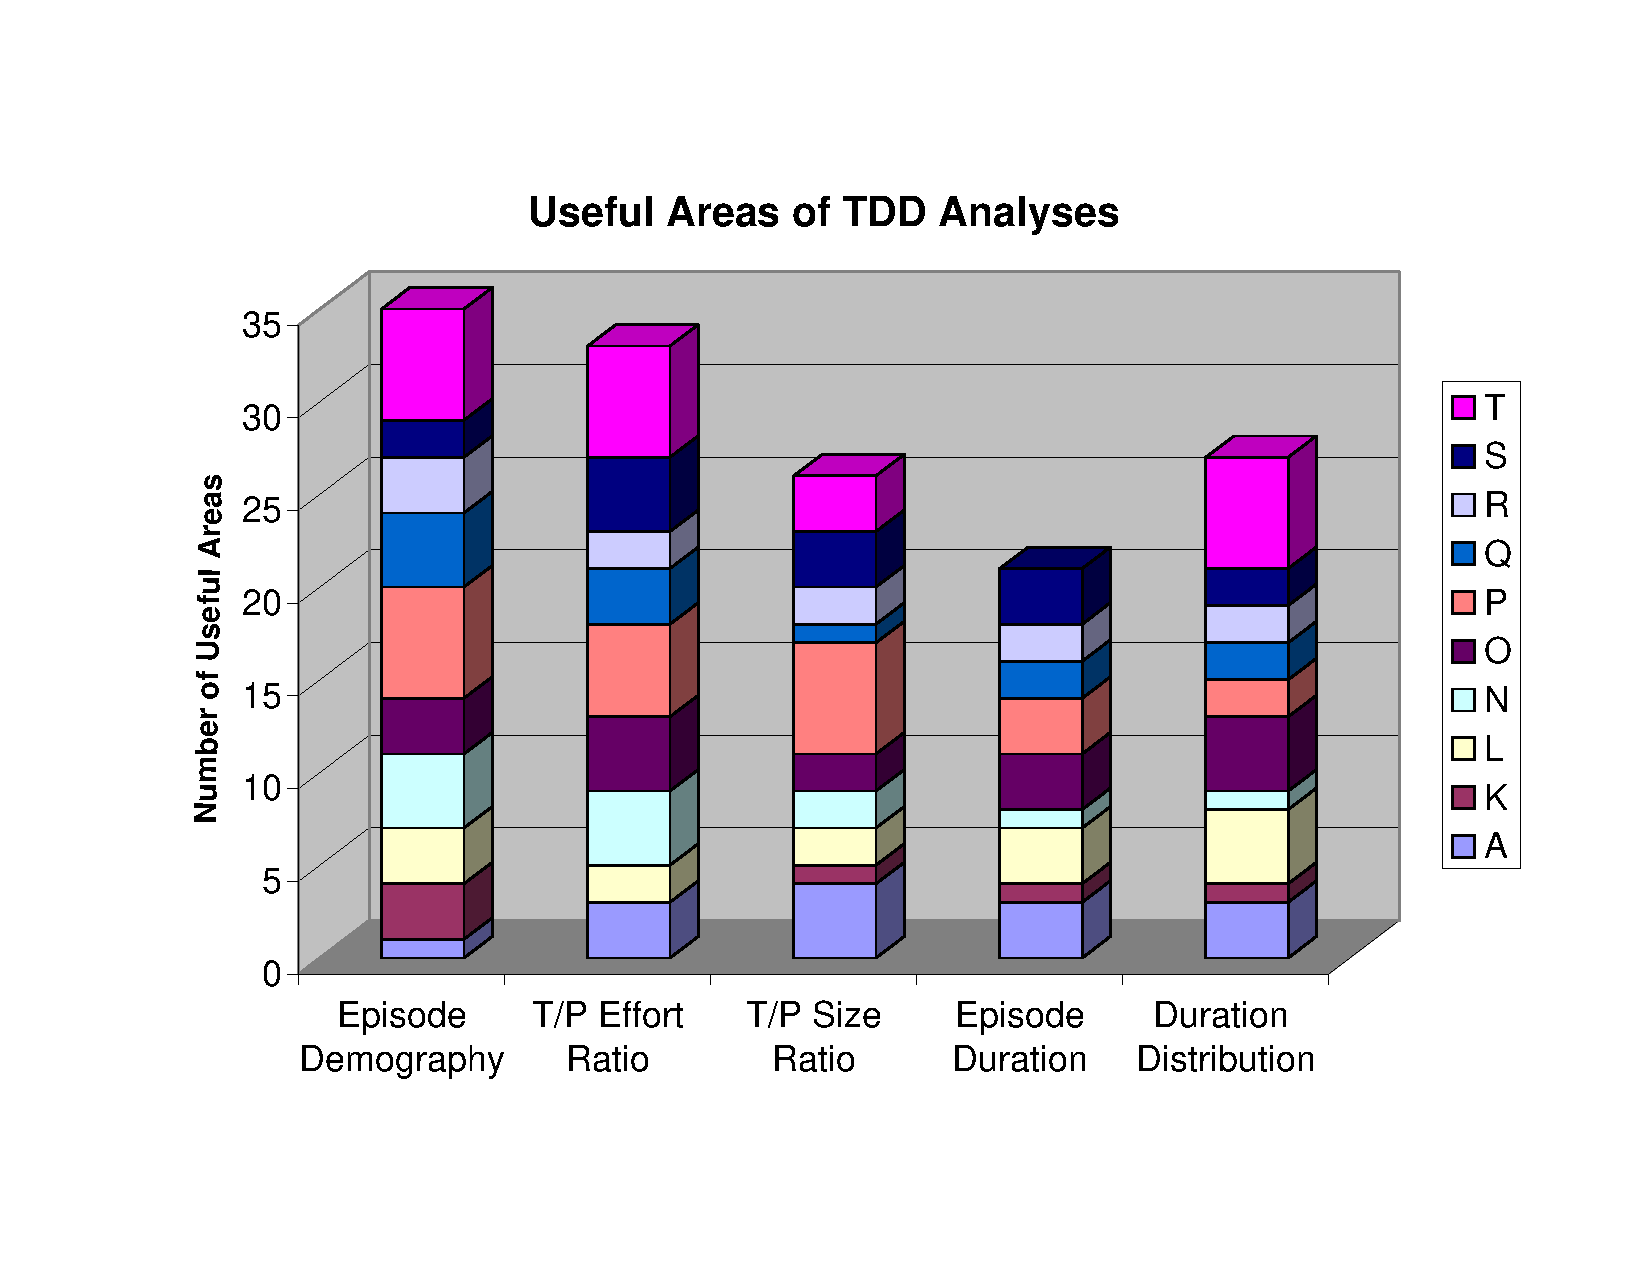
\includegraphics[width=1.0\textwidth]{figs/UsefulnessAreas}
  \caption{Useful Areas of TDD Analyses}
  \label{fig:3DUsefulnessAreas}
\end{figure}
With Figure \ref{fig:3DUsefulnessAreas}, we can easily compare the differences on usefulness among these 5 analyses. The ``Episode Demography'' and ``T/P Effort Ratio'' are the two most useful analyses. Although participants gave the least usefulness score to the ``Duration Distribution'' analysis, it has the potential to be useful basing upon its useful areas 

\subsubsection{Conclusion}
The analysis in this section provided supporting evidence to the research question Q2d. Participants generally agreed that the Zorro is useful and it can be used to understand and improve their TDD practices. %Note that there is a threat to the validity of this conclusion because usefulness evaluation is objective. %It is likely that the participants gave high scores because they did not want to offend me. In the industrial case study, I am going to evaluate it again. Since the participants in that study do not know me, they can freely give their opinions without worrying about being impolite.

\section{Chapter Summary}
\label{sec:discussion}
In this chapter, I validated Zorro's sensor data collection (sections \ref{subsec:SensorDataValidation}) and TDD behavior inference (\ref{subsec:VideoObservationValidation}). Based upon the participant observation analysis, these results provide supporting evidence to research questions Q2a and Q2b (See Chapter \ref{ch:Research}).

In this study, I used participant comments to cross-validate Zorro's inference of development behaviors and TDD compliance. The analysis of their comments (Section \ref{subsec:ParticipantCommentAnalysis}) provided supporting evidence to the research question Q2c. Participants cross-validated that Zorro inferred TDD development behaviors accurately and that participant observation is a reasonable research method for validating Zorro. 

As part of this study, I interviewed participants to survey their opinions on unit testing and TDD. The survey found that participants had a variety of opinions on how useful unit testing and 
TDD are (Section \ref{subsec:ParticipantInterviewAnalysis}). Most of them believed that unit testing and TDD can help to improve software quality. 

Participants also evaluated the usefulness of five TDD analyses provided by Zorro. The usefulness evaluation analysis (Section \ref{subsec:UsefulnessAnalysis}) found supporting evidence to the research question Q2d (See Chapter \ref{ch:Research}). 

In addition, I discovered an unexpected phenomenon (Section \ref{subsec:ParticipantGroup}) in the data analysis. Some participants sometimes forced Eclipse, the IDE I used in this study, to continue test invocations regardless of compilation errors. This behavior impacted Zorro's development stream partitioning and development behavioral inference. In this chapter's data analysis, I termed this development behavior as G2-DevBehavior, and divided participants into groups G1 and G2 for comparison. The validation analyses showed that Zorro's inference accuracy and consistency would improve significantly if Zorro could correctly interpret G2-DevBehavior. Thus it is necessary to let Zorro to allow this development behaviors in the future. 

%In sections \ref{subsec:VideoObservationValidation} and  \ref{subsec:ParticipantCommentAnalysis}, I discussed its effects using the video analysis and participant comment analysis. Even though Zorro yielded acceptable TDD behavior inference results, accommodating the G2-DevBehavior has the promise to improve Zorro's inference capability.
\chapter{Industrial Case Study}
\label{ch:Industry}

The pilot study and the classroom case study show that Zorro can infer TDD when it occurs in the educational and controlled environments. After these two studies, I turned my focus into evaluating Zorro's usefulness for researchers. In order to achieve this goal, I collaborated with Dr. Geir Hanssen, a researcher from SINTEF ICT of Norway on an industrial case study in which Zorro was adopted. My role in this study was the technique supporter of Zorro. I assisted Dr. Hanssen in deploying Zorro to the site and helped him to analyze the collected data. In the end, I interviewed him with regard to Zorro's usefulness.

\section{Purpose of the Study}

The purpose was to test Zorro's usefulness for researchers regardless of the accuracy of Zorro's data collection and correctness of Zorro's inference of TDD development behaviors.

\section{Research Questions}
\label{sec:Industry-Questions}
The specific research question of this study is \textbf{Q3a: How can researchers use Zorro to assist empirical evaluation of TDD?} It supports the overall research question Q2: \textit{``How useful is Zorro?''} 

\begin{comment}
\section{Experiment Design}
\label{sec:Industry-Design}

To answer the above research question, I sent solicitation emails invited TDD researchers to use Zorro in their evaluation studies of TDD. After seeing the demo of Zorro (Section \ref{sec:Industry-Journal-Inception}),  Dr. Geir Hanssen and Dr. Tor Erlend F{\ae}gri from SINTEF ICT of Norway \footnote{ICT stands for Information and Communication Technology, a department of SINTEF. SINTEF is the Foundation for Scientific and Industrial Research at the Norwegian Institute of Technology.} instantly contacted us for the possibility of using Zorro in an evaluation study of TDD. 

 
\subsection{Participants}
Dr. Geir Hanssen and an European software company were the participants of this study. Dr.  Hanssen is a researcher who is interested in studying TDD's impacts on software quality and developer productivity. With this study, he wanted to compare TDD with an existing Test-Last  practice. The software company provides a packaged software product for marketing and customer surveys \cite{Hanssen:06}. In my thesis, I will use Foosball LLC to represent this company for the purpose of anonymity. 

\subsection{Projects}
The Foosball LLC started a TDD project and a Non-TDD project simultaneously in March 2007, both of which were developed in Microsoft Visual Studio .NET Team Edition. The TDD project had 12 developers, and the Non-TDD project had 8 developers. 

\subsection{Instruments}
We instrumented the development processes with the Hackystat Visual Studio .NET sensor, another Zorro compatible sensor that can collect sufficient data for Zorro to infer the development behaviors of TDD. I deployed Hackystat to a server provided by the Foosball LLC company for data collection and analysis. Before the projects started, I wrote a sensor installation guide for each developer. Following these guides, The developers installed the sensor that instrument their development processes.
\end{comment}

%Dr. Geir Hanssen is a researcher from SINTEF ICT of Norway who conducted this study to compare TDD agains an existing TL-practice. The project was divided into two sub-projects: a TDD project and a TLD project. Twelve developers were in the TDD project and 8 developers were in the TLD project. In this study, I deployed a Hackystat 

%conducted a case study in an Europian software company. 
%Unlike the pilot study (Chapter \ref{ch:Pilot}) and the classroom study (Chapter \ref{ch:Classroom}) that evaluated Zorro in controlled environments, the industrial study was a pure case study that has no control over participation, instrument and process management. It was a collaborative research with 

%They want to conduct an evaluation study of TDD in comparison to an existing TL-practice (Test-Last) in a Norwegian software company. They found that collecting process and product data was very hard in practice because the company put maximum pressure on reaching next deadline and did not want anything that does not add direct value to the project, The unobtrusiveness and automated data collection of Zorro 

% They worked with a Norwegian software company that provides a packaged software product for marketing and customer surveys \cite{Hanssen:06}. 

\section{Case Study Journal}
\label{sec:Industry-Journal}

In Fall 2006, Dr. Hanssen planned to conducted an evaluation study of TDD against an existing Test-Last practice in an European software company named Foosball LLC \footnote{The company is real but its name is faked.}. According to Dr. Hanssen, a barrier facing this study was that harvesting development data was very hard. The Foosball LLC agreed to participate in this study but did not want to engage into any research activities that do not add much direct value. So Dr. Hanssen reached us for the possibility to use Zorro in his study, which leads to this collaborative industrial case study. As a facilitator, I provided the technique support of Zorro, assisted the project manager managing sensor installation, and analyzed the development process using the data Zorro collects. To best describe this research, I will use a journal to highlight the collaborative research activities I conducted. 

\subsection{The Prelude of this study}
\label{sec:Industry-Journal-Inception}
After implementing Zorro, I revamped its data collection and inference rules according to research results of the pilot study (Chapter \ref{ch:Pilot}). In Summer 2006, I worked as an intern at the NRC-IIT \footnote{NRC-IIT stands for Institute for Information Technology of National Research Council Canada.} where I collaborated with Dr. Erdogmus \footnote{Dr. Hakan Erdogmus is a Senior Research Officer in the NRC-IIT Software Engineering Group (http://iit-iti.nrc-cnrc.gc.ca/personnel/erdogmus\_hakan\_e.html). He has interests in Software Economics, Agile Software Development, and Software Process Measurement and Awareness.} on classification of TDD development behaviors and inference of TDD compliance. In Fall 2006, under directions from Professor Philip Johnson --- my thesis advisor, and Dr. Erdogmus, I implemented the ``Zorro Demo'' to illustrate Zorro's capabilities for the purpose of recruiting participants.  

\subsubsection{2006-10-30: Zorro Demo}
I applied some TDD analyses Zorro provides to a real TDD programming session and created the ``Zorro Demo''. The demo was implemented in web pages including a start page, six analysis pages and a feedback page. Figure \ref{fig:ZorroDemo} illustrates the start page that has a brief introduction to Zorro, how it works based upon the ``stop light'' metaphor of TDD, and the navigation buttons ``Previous'', ``Demo Home'' and ``Next''.  

\begin{figure}[htbp]
  \centering
  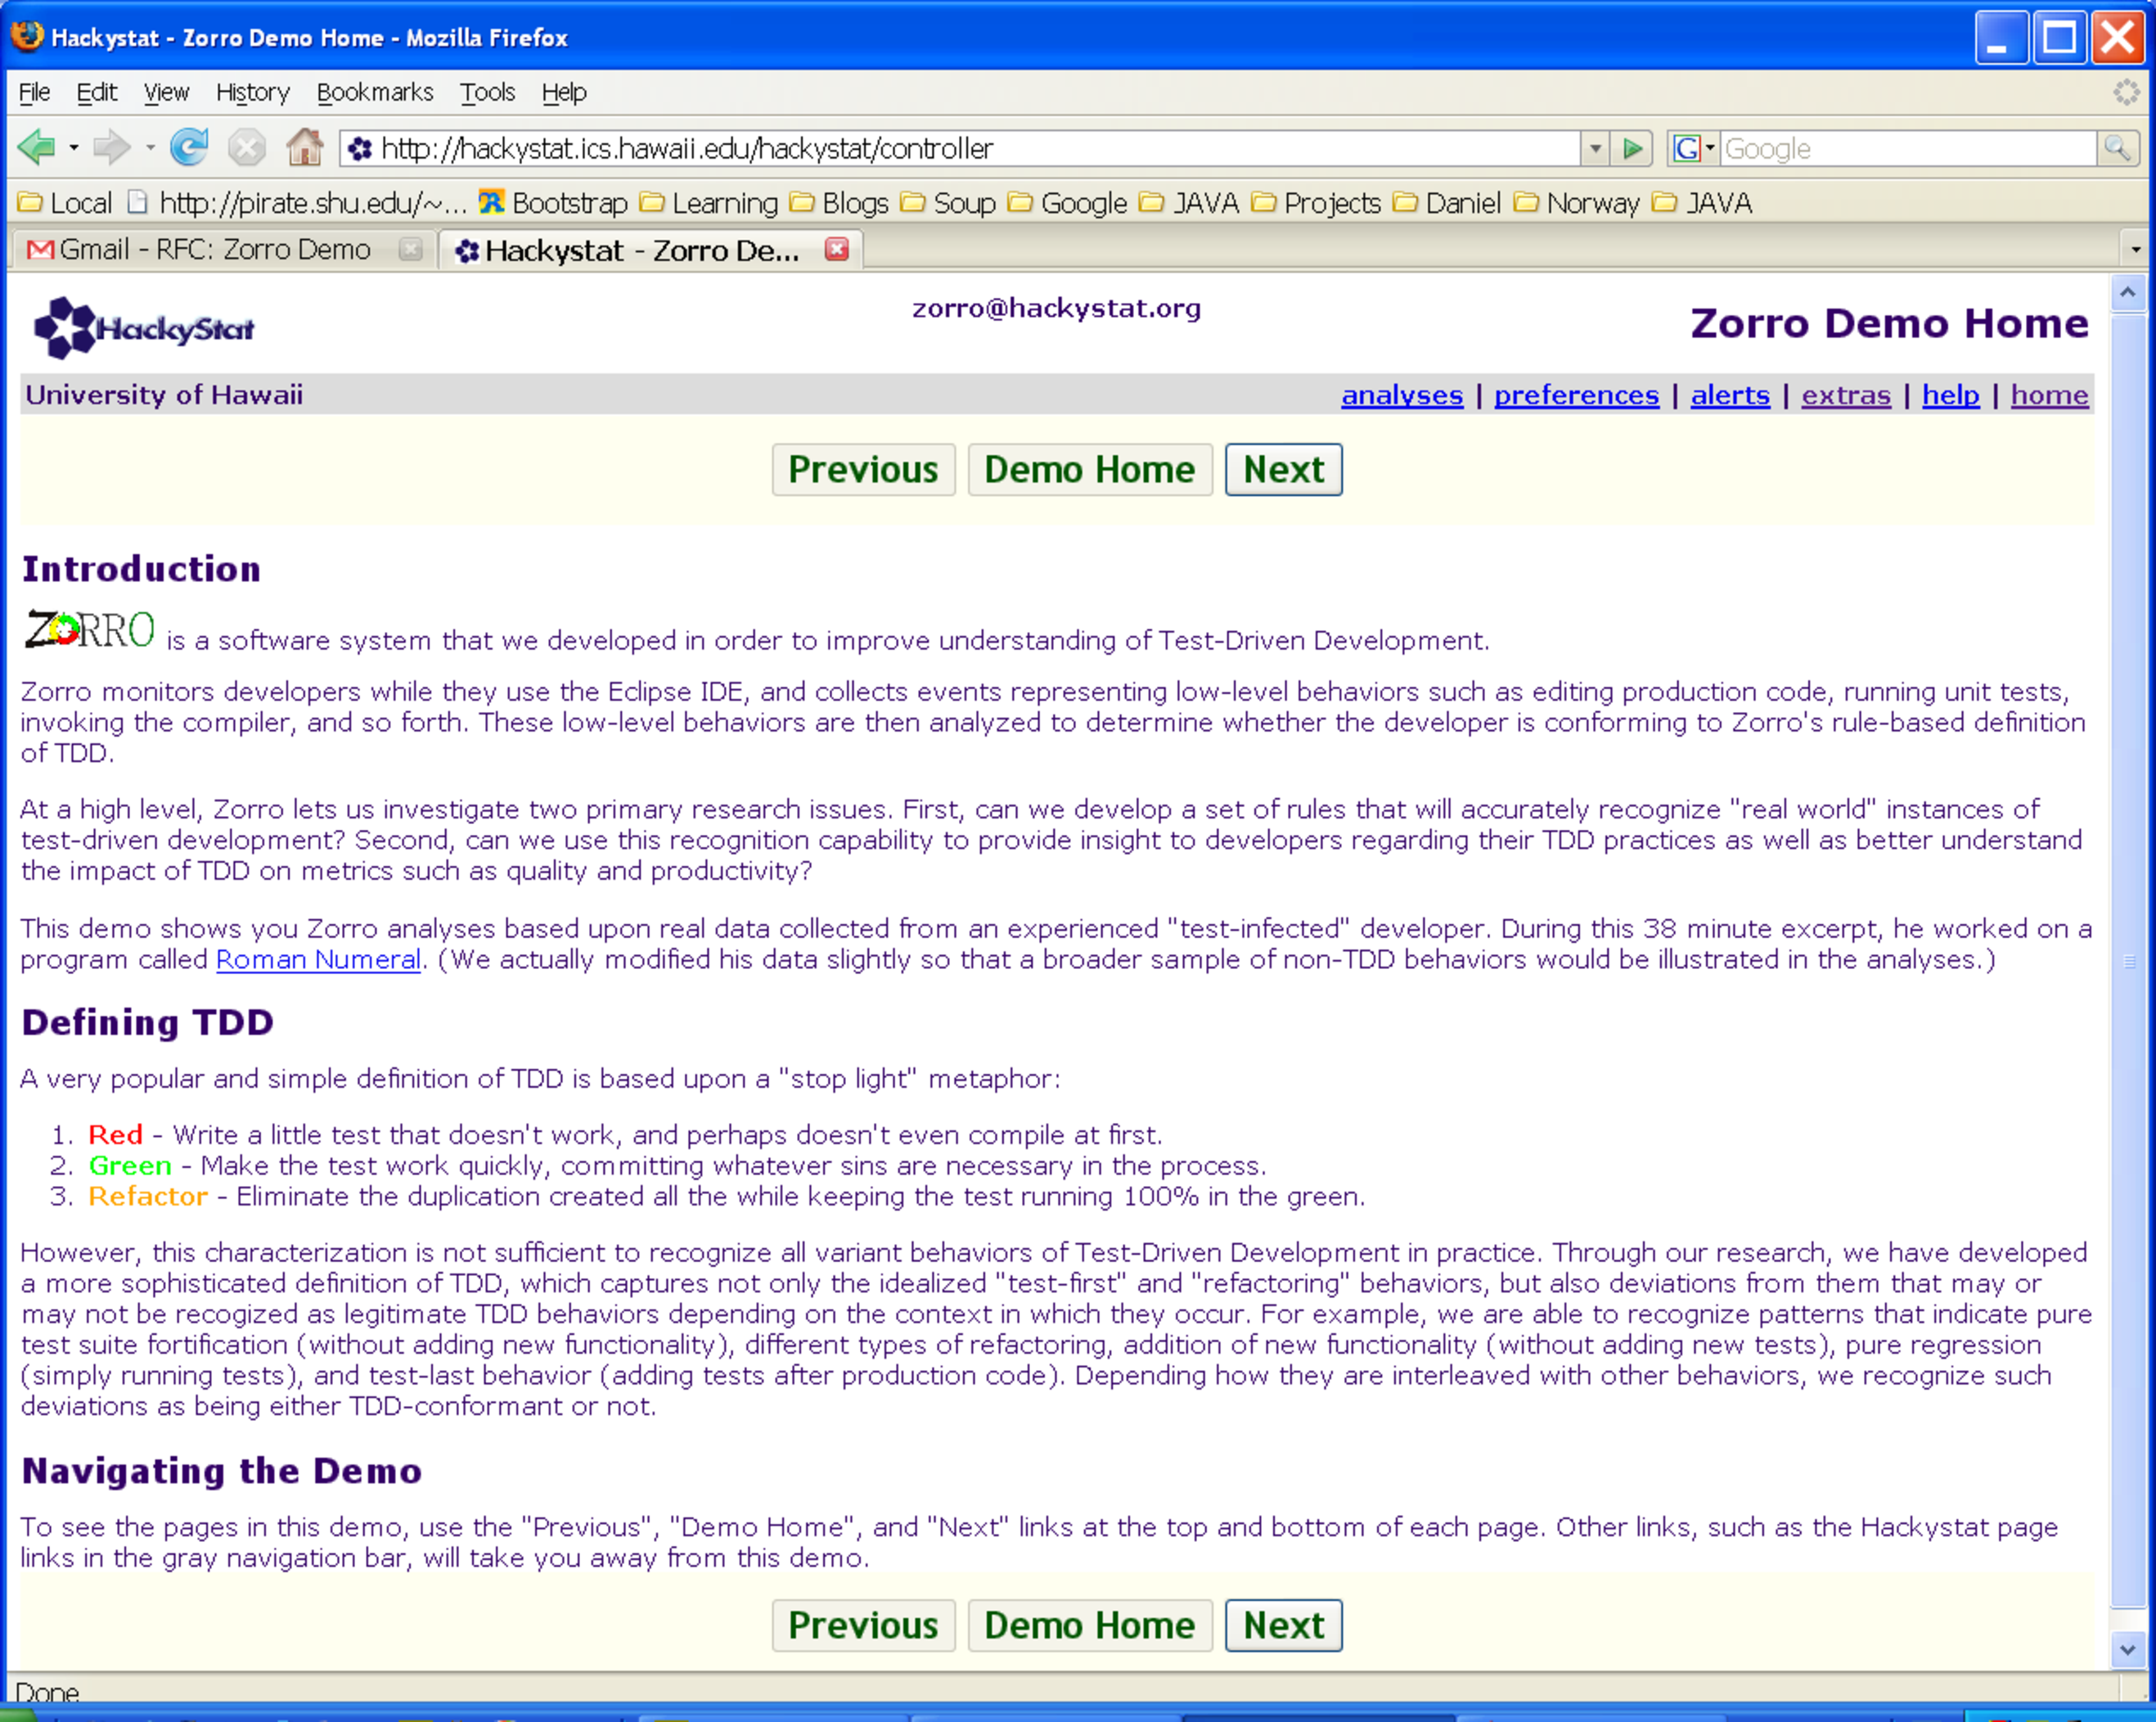
\includegraphics[width=1.0\textwidth]{figs/ZorroDemo}
  \caption{Zorro Demo Wizard}
  \label{fig:ZorroDemo}
\end{figure}

\newpage

\begin{enumerate}
\item{\textbf{TDD Episode Inference}}

Clicking the ``Next'' button in the start page will lead users to the first analysis, ``TDD Episode Inference'' (Figure \ref{fig:ZorroDemoP1}). It provides a view for end users to understand how Zorro infers compliance to TDD using collected development activities. With this analysis, beginners can learn how to program in TDD; experienced practitioners can validate the inference rules and improve their compliance to TDD; and researchers can improve validity of their empirical studies by knowing participants' compliance to TDD. 

\begin{figure}[htbp]
  \centering
  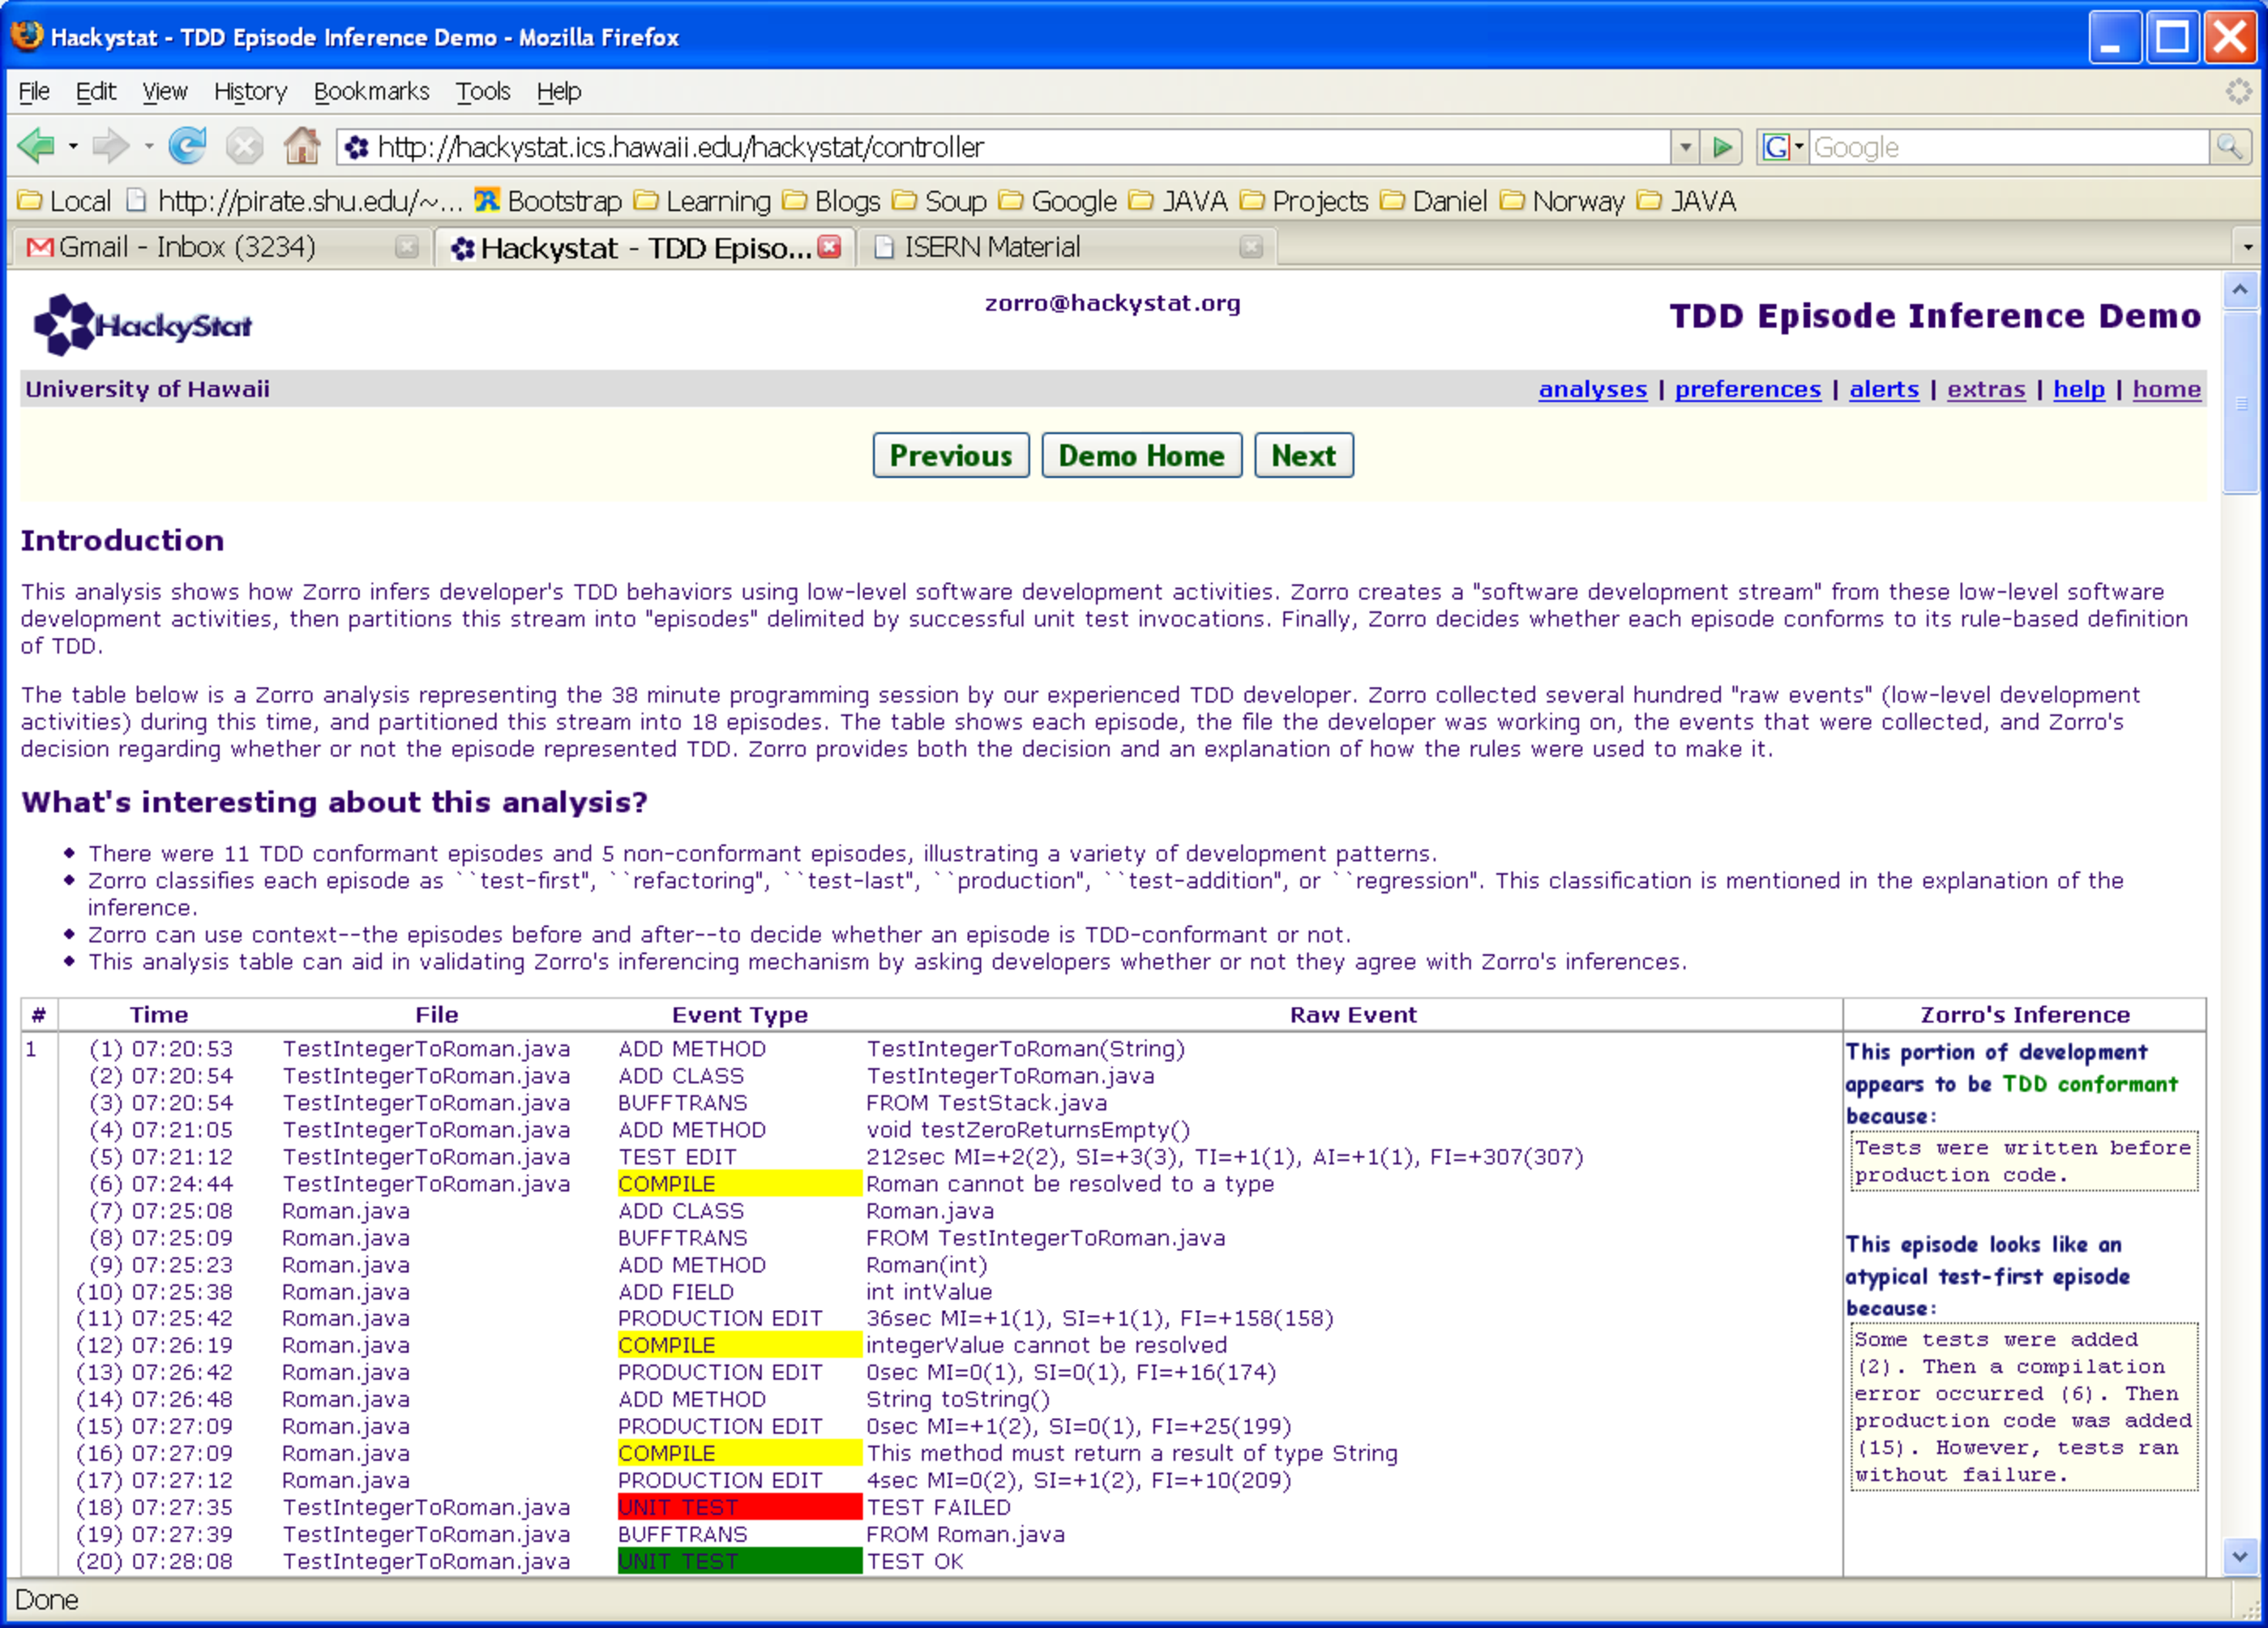
\includegraphics[width=0.9\textwidth]{figs/ZorroDemoP1}
  \caption{TDD Episode Inference Demo}
  \label{fig:ZorroDemoP1}
\end{figure}


\newpage
\item{\textbf{TDD Episode Demography}}

Following ``TDD Episode Inference'' is ``TDD Episode Demography'' that is an overview of a programming session (Figure \ref{fig:ZorroDemoP2}). It lines up all the episodes partitioned from the development stream, each of which is a box with a two-letter acronym representing the episode development behavior. With this analysis, users can inspect TDD programming sessions and look for TDD development patterns for improvement.  

\begin{figure}[htbp]
  \centering
  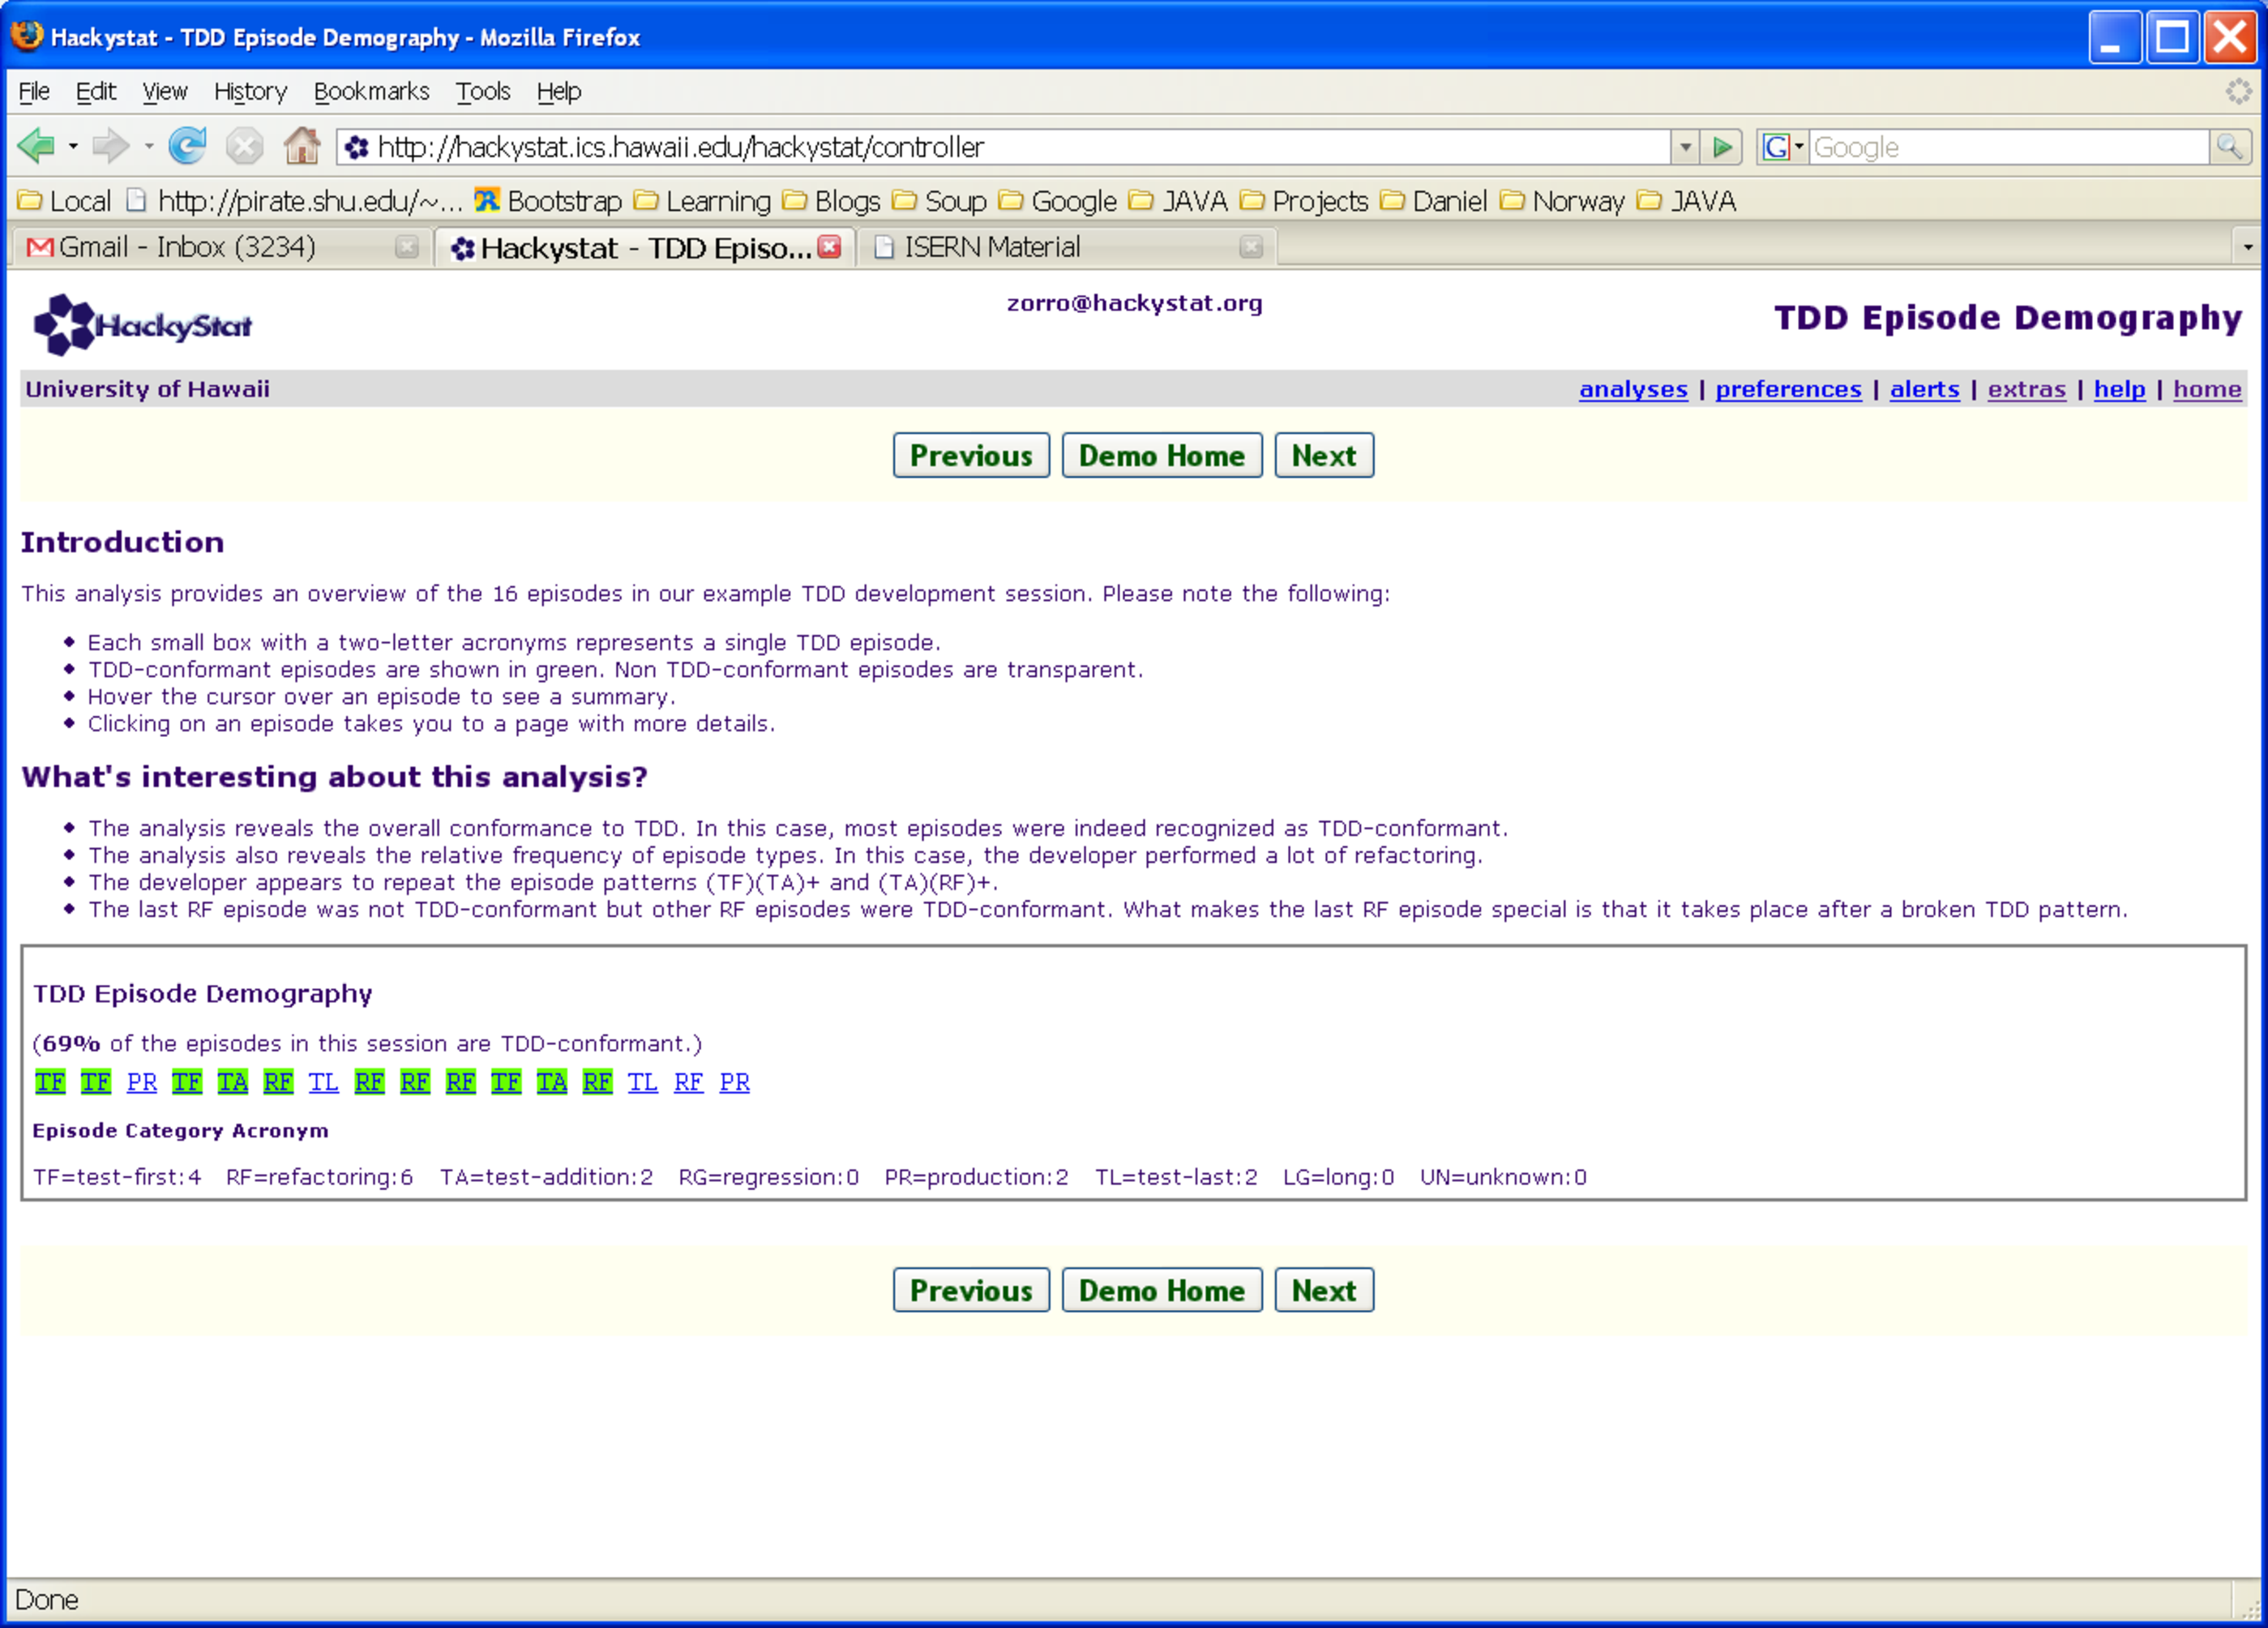
\includegraphics[width=0.9\textwidth]{figs/ZorroDemoP2}
  \caption{TDD Episode Demography}
  \label{fig:ZorroDemoP2}
\end{figure}
In addition to showing overall development behaviors and compliance to TDD, this analysis can interact with the ``TDD Episode Inference'' analysis. When users move mouse over a box in this analysis, a tooltip of episode synopsis will appear on the screen next to the mouse cursor (Figure \ref{fig:ZorroDemoP2X}), and border of the box will change to blue which indicates that it is clickable. Clicking a box will direct users to ``TDD Episode Inference'' (See Figure \ref{fig:ZorroDemoP2X2}). 
\begin{figure}[ht]
  \centering
  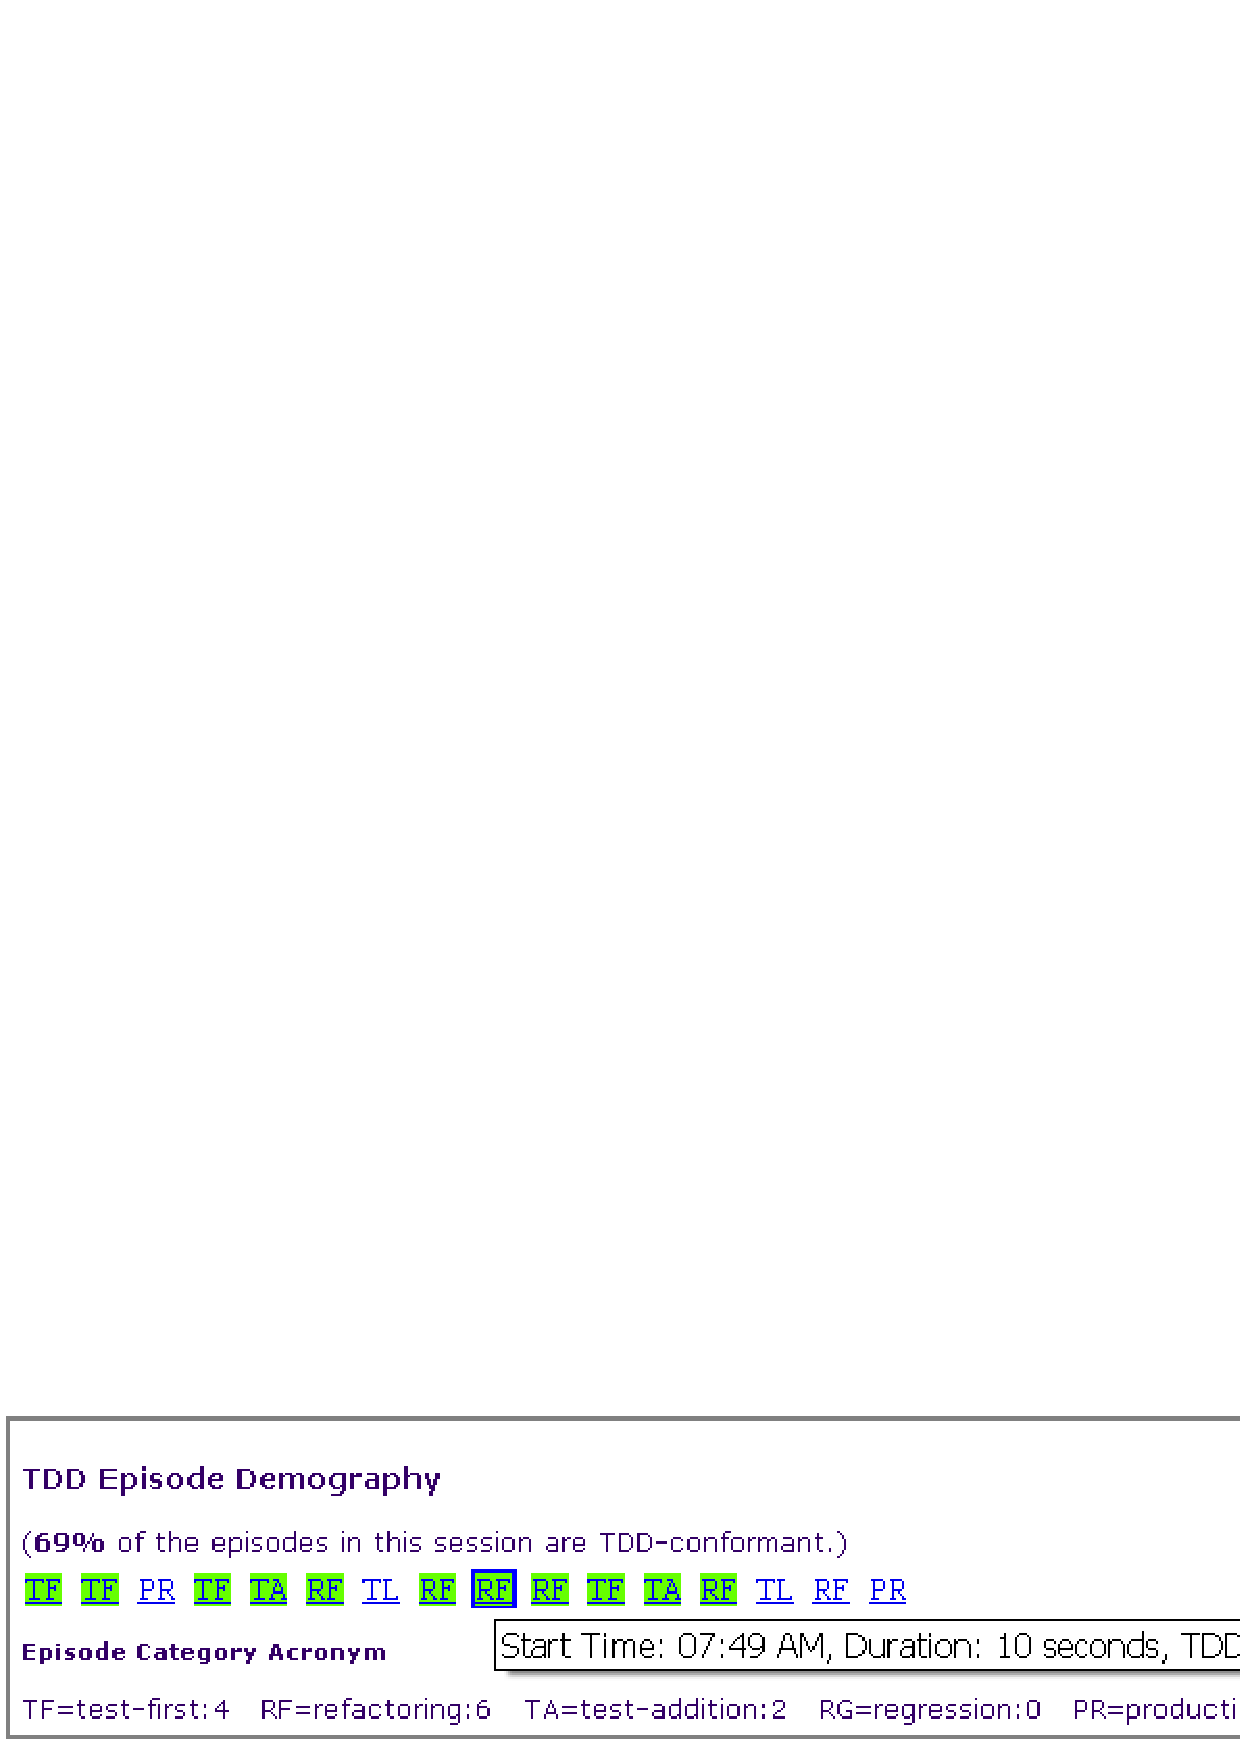
\includegraphics[width=0.9\textwidth]{figs/ZorroDemoP2X}
  \caption{Tooltip of Episode Synopsis}
  \label{fig:ZorroDemoP2X}
\end{figure}
\begin{figure}[ht]
  \centering
  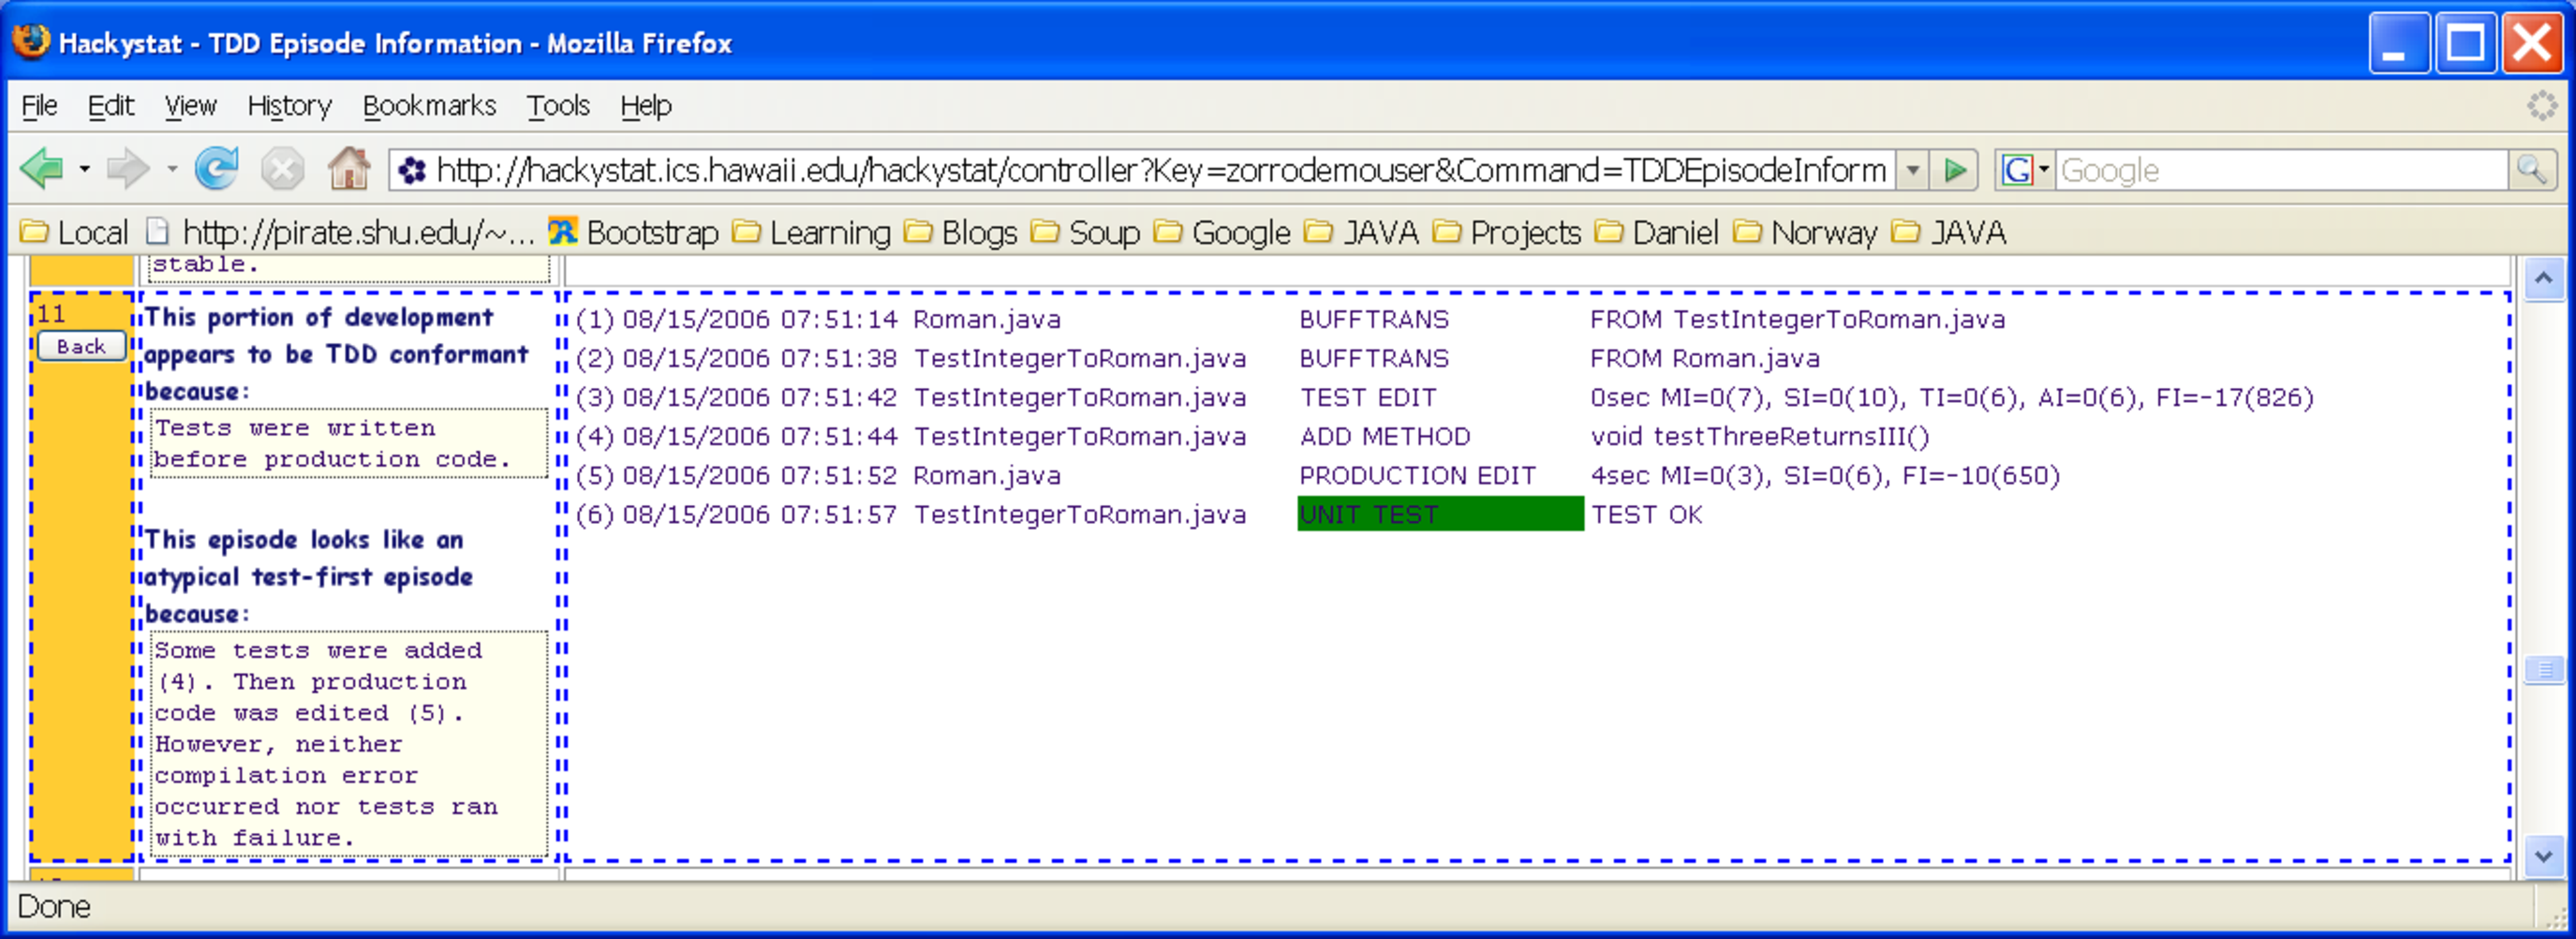
\includegraphics[width=0.9\textwidth]{figs/ZorroDemoP2X2}
  \caption{Episode Details with Back Button}
  \label{fig:ZorroDemoP2X2}
\end{figure}

\clearpage
\item{\textbf{TDD Episode T/P Ratio of Development Time}}

The third analysis is ``TDD Episode T/P Ratio of Development Time'' (Figure \ref{fig:ZorroDemoP3}). This ratio is a good indicator of TDD compliance according to \cite{Wang:04}. %Ideally, equal amount of time should be spent on test and production code if developers faithfully develop software in TDD. 
The drop of T/P ratio could be a warning signal indicating that developers might slip away from TDD. If users are not confident in Zorro's automated inference of TDD compliance, they can inspect their unit testing development activities using this analysis. For others who do not practice TDD but unit testing, this analysis can provide their dynamic unit testing behaviors. 
\begin{figure}[htbp]
  \centering
  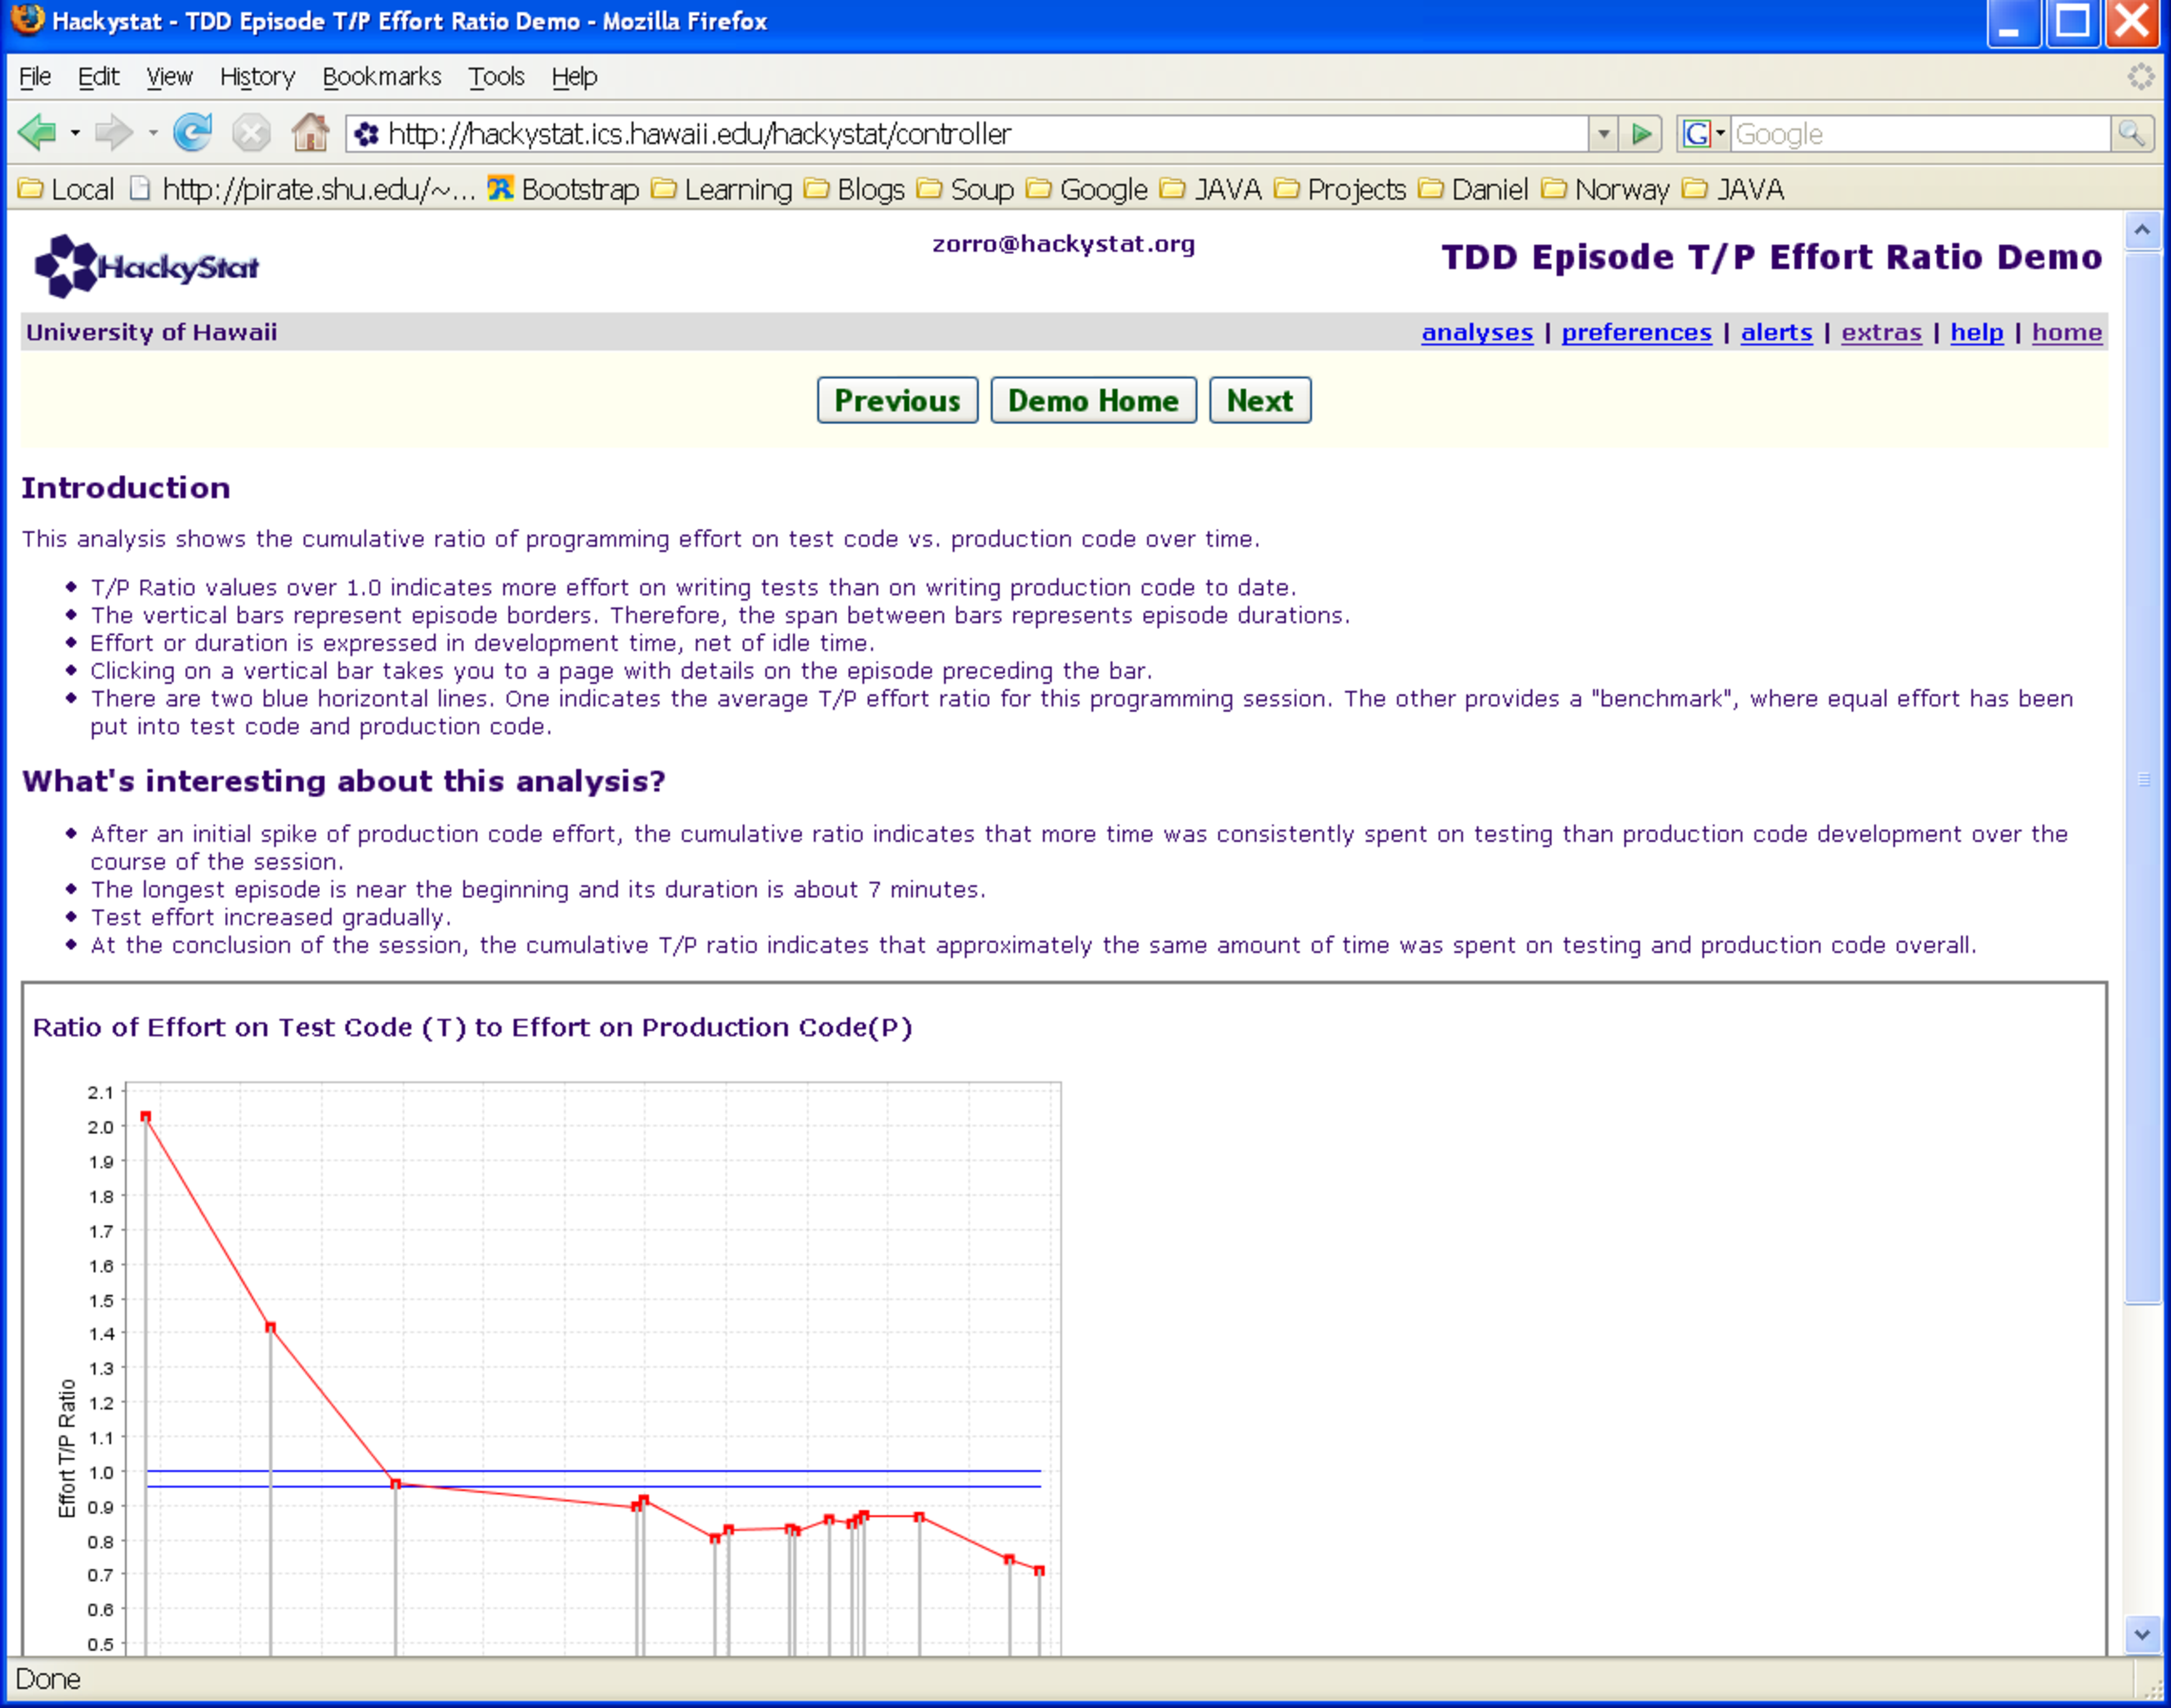
\includegraphics[width=0.9\textwidth]{figs/ZorroDemoP3}
  \caption{TDD Episode T/P Ratio of Development Time}
  \label{fig:ZorroDemoP3}
\end{figure}

\clearpage
\item{\textbf{TDD Episode T/P Ratio of Code Size}}

The fourth analysis is ``TDD Episode T/P Ratio of Code Size'' (Figure \ref{fig:ZorroDemoP4}). Similarly. it provides another metric for measuring TDD compliance. The metric of T/P ratio of code size measures the cumulative net increase of test code and production code relatives. This analysis can easily tell whether test code is written incrementally.

%However, unlike the ratio of development time, T/P ratio of code size can not be connected with the TDD compliance directly. 
\begin{figure}[htbp]
  \centering
  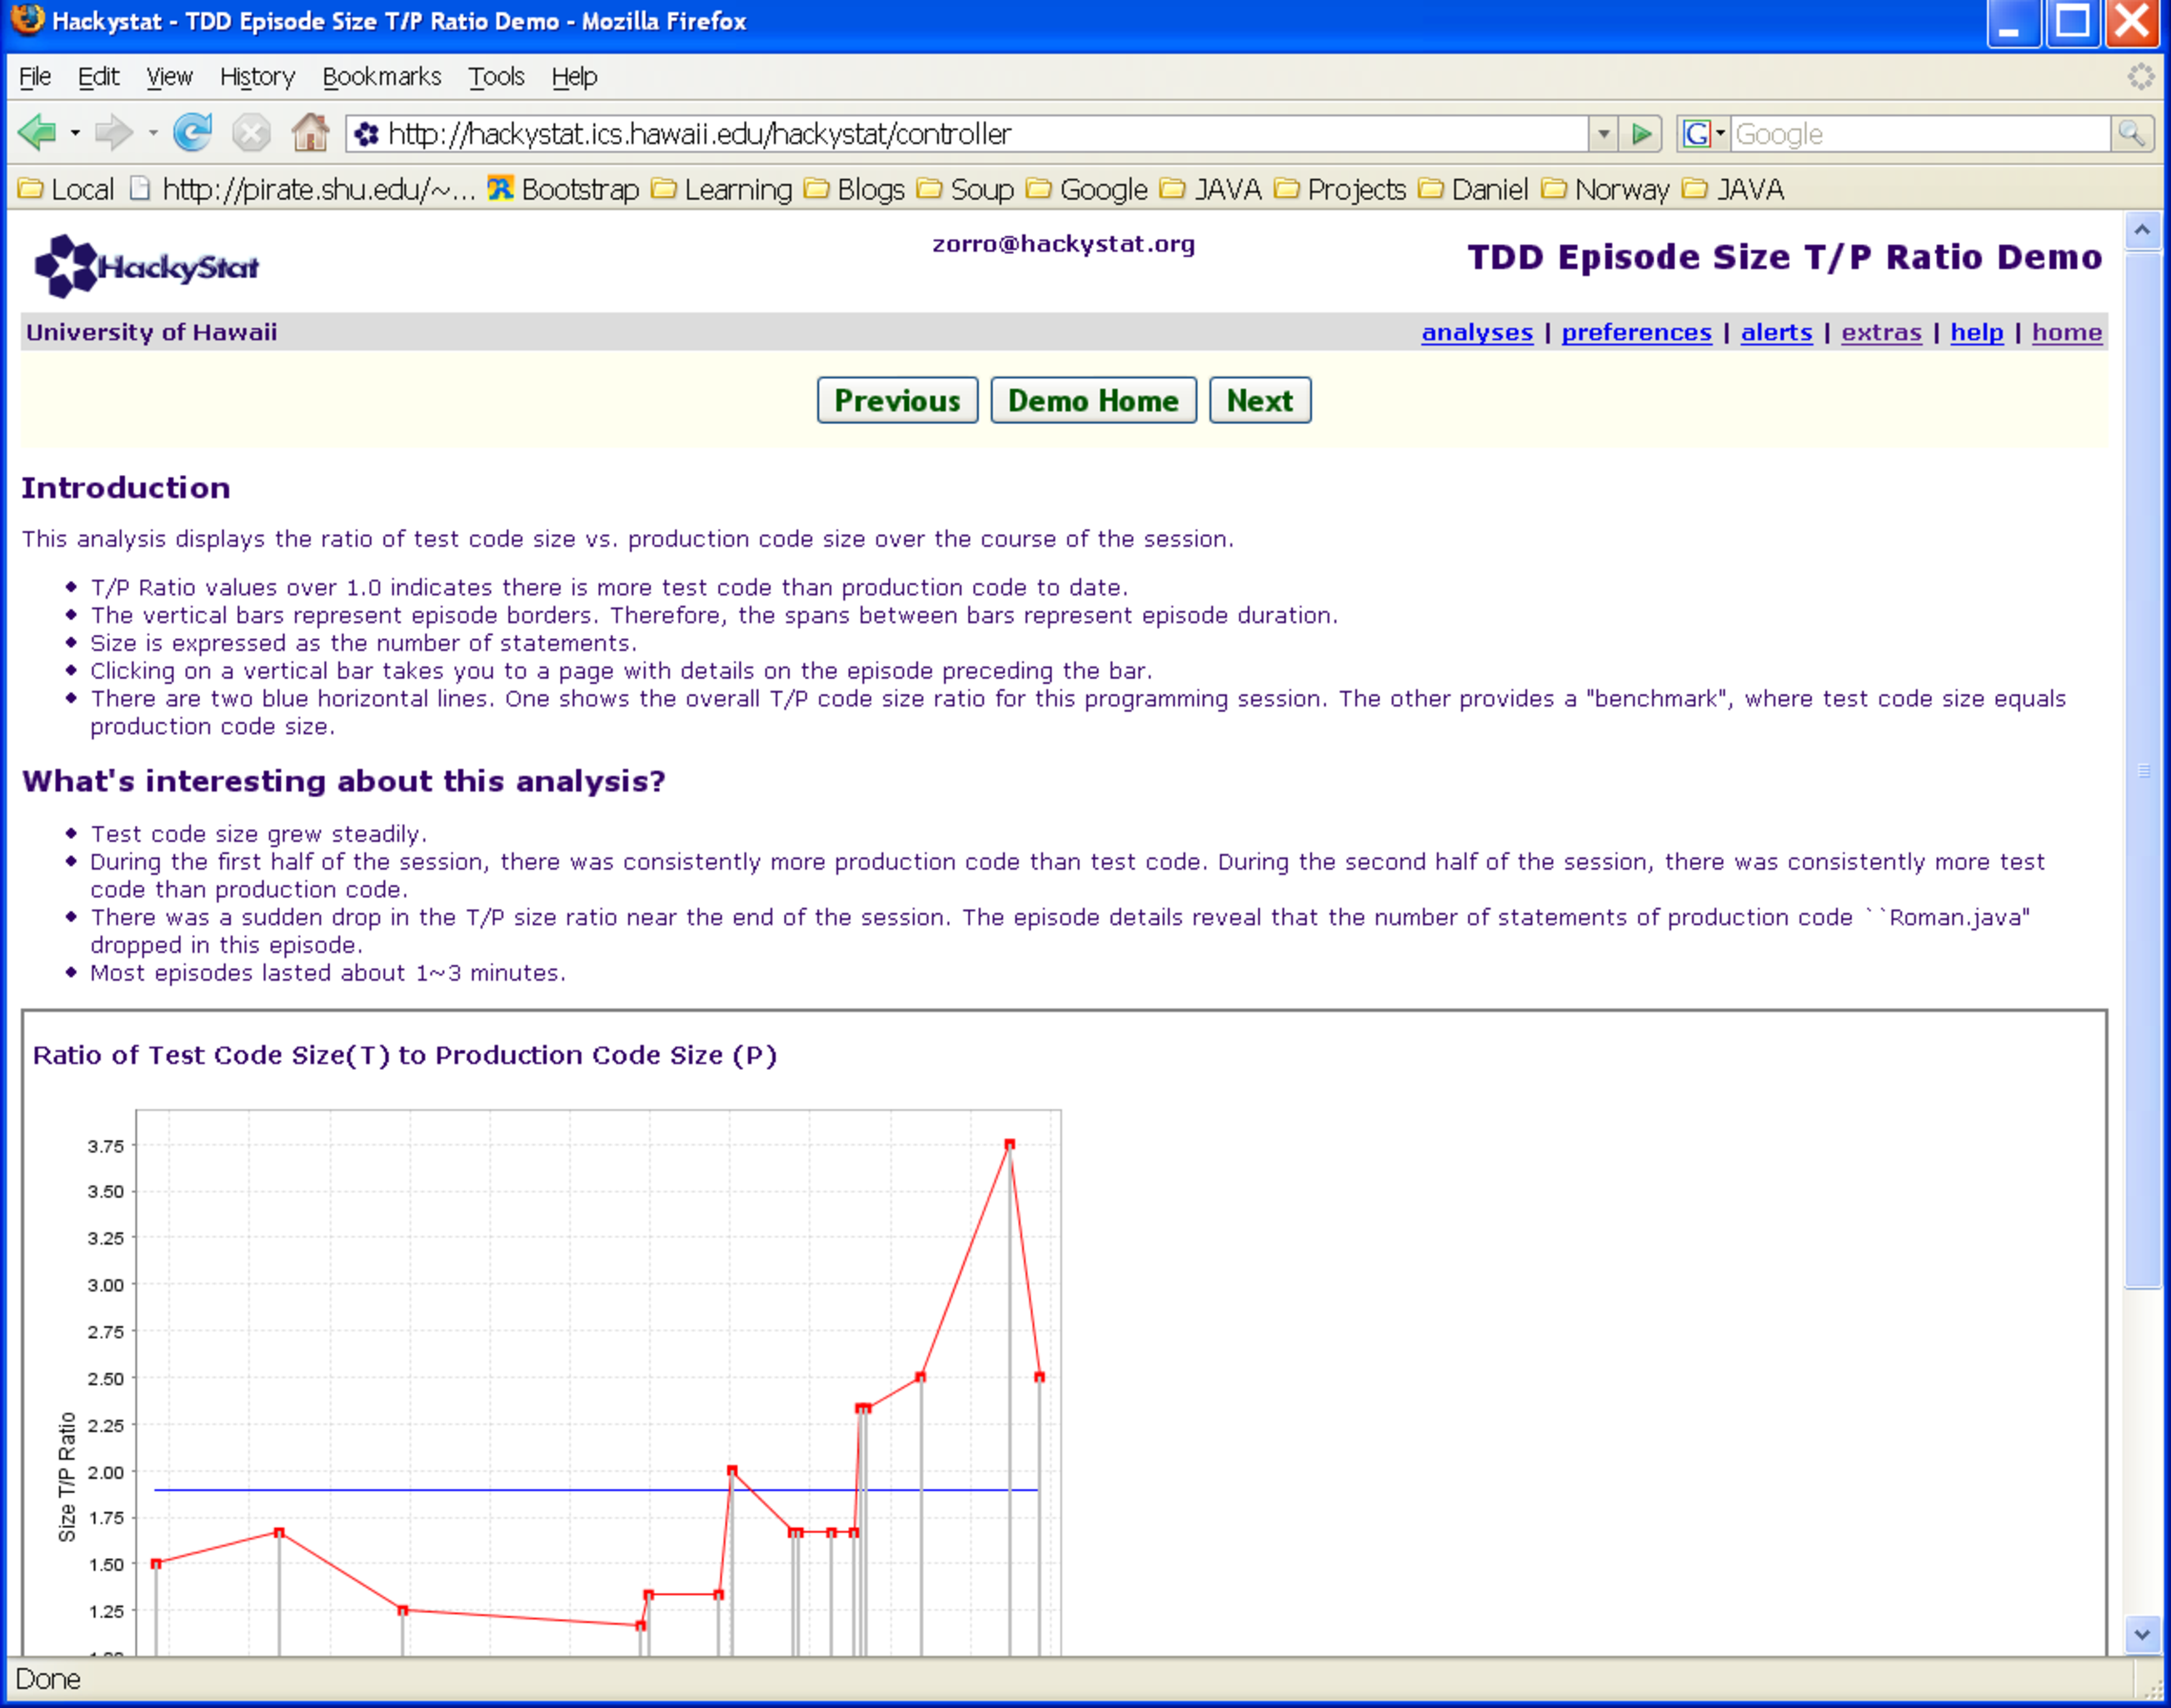
\includegraphics[width=0.9\textwidth]{figs/ZorroDemoP4}
  \caption{TDD Episode T/P Ratio of Code Size}
  \label{fig:ZorroDemoP4}
\end{figure}

%With this analysis, developers can see the moving T/P ratio over a programming session that provides information about TDD compliance too. 

\clearpage
\item{\textbf{TDD Episode Duration}}

The fifth analysis is ``TDD Episode Duration''. How often should developers invoke unit testing is a grey area of TDD. A general consensus is that an iteration of TDD should not last more than ten minutes; otherwise, the process is not agile. In Zorro, I provide the ``TDD Episode Duration'' analysis as a validation tool to observe duration of TDD iterations. It is reasonable that most episodes in TDD are short in length of duration. 
%Kent Beck stated that the occasional long iteration is not a violation to TDD \cite{Beck:03}. 
\begin{figure}[htbp]
  \centering
  \includegraphics[width=0.9\textwidth]{figs/ZorroDemoP5}
  \caption{TDD Episode Duration}
  \label{fig:ZorroDemoP5}
\end{figure}


\newpage
\item{\textbf{TDD Episode Duration Bins}}

The last analysis is ``TDD Episode Duration Bins''. Simply as its name indicates, this analysis puts episodes into a set of bins according to their duration. Each bin defines a range of duration. In Figure \ref{fig:ZorroDemoP6}, the vertical axis is for numbers of episodes that fall into each bin. 
\begin{figure}[htbp]
  \centering
  \includegraphics[width=0.9\textwidth]{figs/ZorroDemoP6}
  \caption{TDD Episode Duration Bins}
  \label{fig:ZorroDemoP6}
\end{figure}

To the TDD programming session analyzed in this demo, most episodes fell into bins of short durations according to Figure \ref{fig:ZorroDemoP6}. 

\clearpage
\item{\textbf{Zorro Demo Feedback}}

The last page of the ``Zorro Demo'' is ``Zorro Demo Feedback'' that invites readers to collaborate on studying TDD. With this demo, we targeted at three kinds of users: TDD beginners, experienced TDD practitioners, and TDD researchers. After reading information about collaborative research opportunity with us, readers can provide feedback to us using the box included in this page (Figure \ref{fig:ZorroDemoP7}). 

\begin{figure}[htbp]
  \centering
  \includegraphics[width=0.85\textwidth]{figs/ZorroDemoP7}
  \caption{Zorro Demo Feedback}
  \label{fig:ZorroDemoP7}
\end{figure}

\end{enumerate}

\clearpage
\subsubsection{2006-11-07: Feedback from ISERN}
As the first step to find collaborative opportunity with researchers of TDD, we sent an RFC of Zorro Demo to the ISERN mailing list that contains researchers from worldwide who are interested in empirical software engineering research. On the same day we sent this collaboration solicitation email, Dr. Geir Hanssen and Dr. Tor Erlend F{\ae}gri from SINTEF ICT of Norway gave  very positive feedback on Zorro, and expressed that they were very interested in using Zorro in a comparative study between TDD and an existing Test-Last practice. 

They planned to conduct this study under the assistance from an European software company by harvesting data such as time spent for testing/coding, test code size/production code size etc. They were also interested in finding ways of validating any effect that the TDD-practice may have on product quality, speed of production, and also potentially on code quality (maintainability, code design-style and others). However, doing these was very hard in practice because the software company did not want to be disturbed when developers put maximum pressure on reaching the release deadline. As a result, collecting data became a problem in this already planned study. Thus, automated data collection became tempting and Zorro is such a tool that can bring immediate values to them.

Although Zorro was a good fit to this study, the software company used Visual Studio .NET rather than Eclipse, and the programming language was C\# rather than Java. A minimum set of sensor data types (See Table \ref{tab:Zorro.Sensors}) are required in order for Zorro to function. Unfortunately, the Visual Studio .NET senor was very premature and it can only collect a few of them. Thus, if we wanted to engage in this study, the most imperative task was to develop a Visual Studio .NET sensor that can collects necessary sensor data types. Moreover, the sensor had to be implemented and tested in a very short time frame since the software company planned to start the project in January 2007.

\subsection{Preparation}
\label{sec:Industry-Journal-Preparation}
With confidence in Zorro and our software development skills, we decided to participate in this collaborative industrial case study. The preparation tasks include implementation of the Visual Studio .NET sensor and installation of Hackystat.

\subsubsection{Visual Studio .Net Sensor Implementation}
We exchanged several emails with Dr. Hanssen to understand the company's development environment in December 2006. %It occurred to us that the Visual Studio .NET had a new version released in 2005, which has built in support of unit testing. 
With the help from Qin Zhang, another Ph.D student who was also my colleague in CSDL, I implemented the Visual Studio .NET sensor that was Zorro-compatible. After developing the sensor, I tested that Zorro can infer TDD development behaviors occurred in the IDE of Visual Studio .NET.  

\subsubsection{Hackystat Server Installation}
Zorro runs on the server-side of Hackystat. Foosball LLC provided a dedicated server for this study. Using Windows' Remote Desktop application, I logged into the server, installed and configured a Hackystat server for this case study in February 2007.

\subsection{Collaborative Research Activities}
In March 2007, the company launched both the TDD project and the Non-TDD project with 20 developers, twelve of which developed in TDD. I assisted developers installing the Visual Studio .NET sensor, which collected development activities in the background unobtrusively. Periodically, I analyzed the collected data and generated technique reports for Dr. Hanssen and the project manager regarding developers' development behaviors.

\subsubsection{2007-02-22: Sensor Installation Instruction}
Pertaining to the least possible interruption to the development process required by the participated company, I wrote a script to automate the sensor installation for developers. Figure \ref{fig:VSTE-Sensor-Script} illustrates the output from this script when a developer invoked this script. For each developer, I sent an individual email to him/her with customized installation instructions. Only one developer encountered difficult in installing the sensor due to his customization of the Windows user profile. I fixed this by patching the installation script. 

\begin{figure}[htbp]
  \centering
  \includegraphics[width=1.0\textwidth]{figs/VSTE-Sensor-Script}
  \caption{Output of Visual Studio .NET Sensor Installation Script}
  \label{fig:VSTE-Sensor-Script}
\end{figure}

\subsubsection{2007-02-28: \#1  admin guide and sensor installation status}
The admin guide is a document for Dr. Hanssen and the project manager to use Hackystat and Zorro. This document covers following contents:
\begin{itemize}
\item Login as the administrator, 
\item Login as any developer,
\item Check sensor installation status (days with sensor data),
\item Check a developer's collected development activities,
\item Invoke the analyses described in the Zorro Demo.
\end{itemize} 
Following this guide, they can login as the administrator, check received data, define Hackystat projects, and invoke Zorro's analyses. 

I also summarized the sensor installation status based on data received on the server. According to this report, two developers successfully installed the sensor within a day after I sent the instructions to them. 

\subsubsection{2007-03-02: \#2 admin guide }
I updated the admin guide on March 2, 2007. According to this guide, some developers sent data to the Hackystat server. After observing the collected data, I registered projects for developers who installed the sensor so that the project manager can use Zorro to analyze their  development behaviors. 

When writing the sensor installation status report, I was surprised to find that none of developers invoked any unit tests. The project manager noticed this as well and asked us whether the sensor worked correctly with TestDriven.NET add-in. Unfortunately I never knew that developers ran tests with TestDriven.NET, a third-party add-in to the Visual Studio .NET. Later, we discovered that some emails from the project manager sent in January 2007 were discarded by the mail server of the University of Hawaii as SPAMs for unknown reasons. I configured my SPAM settings to allow emails sent from the software company, but I had to enhance the sensor to support TestDriven.NET quickly in order to continue this collaborative research. 

\subsubsection{2007-03-05: Support for TestDriven.Net and Sensor Upgrade}
TestDriven.NET was an open source project initially but turned into a proprietary Visual Studio add-in. It is not as extensible as the JUnit plugin of Eclipse so that a third-party observer can not listen to invocations of unit testing. Perhaps because Microsoft started a legal issue against him, the author of TestDriven.NET did not respond to my request for help. Soon I discovered an approach to capture and parse test running results from TestDriven.NET by observing the console output in Visual Studio .NET. After some extensive testing, I released a new Visual Studio .NET sensor for this collaborative industrial case study. %The Foosball LLC was very unhappy with this sensor upgrade but there was no alternatives if we wanted to continue this research. 

It was a little pity that the project manager was very unhappy with this update but there was no alternatives if we wanted to continue this research. As a result, some developers did not install this upgrade according to my observation of the server status. I addressed this issue in the following reports I wrote.

%, and we did not get further answers to our questions regarding their development process. 

\subsubsection{2007-03-20: \#3 sensor installation status}
I updated the sensor installation status report on March 20, 2007. According to this report, 20 developers fell into five groups:
\begin{itemize}
\item {\textbf{Group 1: Those who are successfully using the system}}

Four developers are sending coding and testing data regularly, indicating the sensor is installed and updated.

\item {\textbf{Group 2: Those who need to install the sensor}}

Four developers have not sent any data. They appear to have not installed the sensor at all or are not programming.

\item {\textbf{Group 3: Those who might have uninstalled the sensor}}

Four developers sent data at the beginning but have not sent any data recently. They have either uninstalled the sensor or are not programming.

\item {\textbf{Group 4: Those who might need to update the sensor}}

Four developers are sending coding data but not testing data. Either they are not testing, or have not updated the sensor.

\item {\textbf{Group 5: Those who apparently need to update the sensor}}

Four developers are sending coding data and testing data, but the test data lacks path information indicating the need to upgrade the sensor.

\end{itemize}

Because I conducted this study off-site, the above categorization of developers was only based upon my observation of data received on the Hackystat server. The project manager generously agreed to have developers update the sensor following my suggestions made in this report.  

\subsubsection{2007-04-14: \#4 introduction to the TDD telemetry analyses}

In the report I wrote on April 14, 2007, I introduced the TDD telemetry analyses (See Section \ref{sec:Zorro-Analysis-Telemetry}) to Dr. Hanssen and the project manager. In addition, I defined two Hackystat projects for them. One project was ``The-TDD-Project'' which includes all programmers who developed in TDD as project members, and the other project was ``The-NON-TDD-Project''.  With these two projects, they can invoke TDD telemetry analyses to compare the TDD project and the Test-Last project. A list of TDD telemetry analyses is in the following.

\begin{itemize}
\item {\textbf{DevTime-Chart:}} computes development time developers spent in the Visual Studio .NET environment.  
 
\item {\textbf{DevTime-Members-Chart:}} computes and plots all project members' development time spent in the Visual Studio .NET environment.

\item {\textbf{DevTime-TotalProductionTest-Chart:}} computes and illustrates total development time, the portion on coding, and the portion on testing. 
 
\item {\textbf{EpisodeDurationAverage-Chart:}} illustrates the average episode durations.

\item {\textbf{TDD-Percent-Chart:}} reports the percentage of a project's TDD compliance.
 
\item {\textbf{TDD-All-Members-Chart:}} reports and compares project members' TDD compliance.

\item {\textbf{TDDPercent-And-DevTime-Chart:}} combines the TDD compliance percentage and development time to a given project.
\end{itemize}

Basically this report opened a door to Zorro and Telemetry for Dr. Hanssen and the project manager. With the sensor data collected from developers, Zorro can be used to not only infer developers' TDD development behaviors but also conduct comparative study between TDD and Non-TDD.  

According to feedback received from Dr. Hanssen regarding this report, the number of programmers producing data was disappointing, and he would contact the project manager directly for possibility to improve it. However, he viewed this study as a pilot and planned to replicate it in another software company, which might have a better start and more complete data. Also, other researchers are interested in Zorro's automation of data collection and development behavior inference. 

\subsubsection{2007-05-04: \#5 Comparison Between TDD and Test-Last Projects}
I used Zorro's TDD telemetry analyses to compare development behaviors between the TDD project, and the Test-Last project and wrote a technique report on May 4, 2007. The main points included in this reports are:

\begin{itemize}
\item {\textbf{TDD-Percent-Chart (by development time)}}

The ``TDD-Percent-Chart'' telemetry analysis computes and plots percentages of development time that developers complied to TDD based upon Zorro's inference. Partially due to the imperfect sensor installation, developers did not comply to TDD faithfully in this study. The compliance percentage was 5\% at the best on the weekly basis.

Living far from developers who participated in this study, I did not have the capabilities to investigate causes for the low TDD compliance rate. Perhaps developers did not have the necessary skills to use TDD on their development tasks, or they modified TDD according to their needs. 

\item {\textbf{TPRatio-DevTime-Chart}}

The ``TPRatio-DevTime-Chart'' telemetry analysis is a metric for measuring effort developers devoted to testing. It was interesting to note that developers who were in TDD project evenly divided their effort on testing and production code. On the contrary, developers in the Test-Last project did not test much at the beginning but gradually caught up unit testing. 

\item {\textbf{DevTime-TotalProductionTest-Chart}}

The ``DevTime-TotalProductionTest-Chart'' telemetry chart analysis plots cumulative effort spent on test and production code. According to this analysis, the TDD project had larger growth rate of test code while the Test-Last project had larger growth rate of production code. 

\item {\textbf{DurationAverage-Chart}}

The ``DurationAverage-Chart'' telemetry analysis illustrates how frequently developers invoked unit tests. Interestingly, the episode durations average of the two projects are far longer than 10 minutes.  

\end{itemize}

In addition to the telemetry report, I updated the sensor installation status with development time and T/P ratio for each developer. After reading this report, Dr. Hanssen were more concerned about the legitimacy of the data rather than the hypotheses I claimed regarding the development process. Unfortunately, the project manager concentrated on the software development and did not respond to this report. 

\subsubsection{2007-05-25: \#6 Comparison Between TDD and Test-Last Projects}
Based on the report I wrote on May 25, 2007, developers in the Test-Last project started putting more effort on testing than effort on production code, in contrast developers in the TDD project evenly divided their effort on testing. 

\subsection{Phone Interview with the Researcher}
By the time I write this chapter, developers in Foosball LLC are still working on the software to make the next release. In this research, I installed and configured a Hackystat server for them, developed the Visual Studio .NET sensor, managed the Hackystat server, and wrote six technique reports for the researcher and the project manager. After four months collaboration, Professor Philip Johnson and I interviewed the researcher on July 3, 2007. Table \ref{tab:InterviewStructure} lists the structure of this interview.
\begin{table}[!ht]
\centering
\caption{Structure of the Interview with the Researcher}
\begin{tabular}{|l|l|} \hline
Interviewer & Hongbing Kou, Philip Johnson  \\ \hline
Interviewee & Geir Hanssen \\ \hline
Instrumentation & Voice Recorder \\ \hline
Method      & Phone \\ \hline
Time        & 9PM July 3, 2007 \\ \hline
Length      & 45 minutes \\ \hline
Location    & Collaborative Software Development Laboratory \\ \hline
\end{tabular}
\label{tab:InterviewStructure}
\end{table}

In the interview, we mainly focused on the experiment details behind the scene as well as the researcher's experience regarding this collaborative research. 

\begin{itemize}
\item {Research Background}

It is interesting to note that the Foosball LLC was not specially recruited to participate in this comparative study of TDD. The company worked with Dr. Hanssen before on studying Evo Agile, an agile process that the company has adopted. For whatsoever reason, the company decided to include TDD in its software process and so this case study was initiated. After seeing the Zorro Demo, Dr. Hanssen suggested that they use Zorro for data collection in this study. Because of the unobtrusiveness of Zorro's data collection, the Foosball LLC agreed to have its process instrumented. 

\item {TDD Conformance}

The TDD compliance percentage of this study was very low according to Zorro's inference. However, probing the development process to understand the situation was impossible for me and Dr. Hanssen as well at this moment. Typically, the Foosball LLC has good reputation in complying to what they agreed to, but meeting the deadline has the top priority. It is worthwhile to note that Evo Agile, the software process that the company is using, has tight and well scheduled development activities. TDD is an extra addition to the process, which might help to explain why the project manager did not respond to our requests for understanding their software process.  

\item {Concerns on Sensor Installation}

In the \#3 report of ``Sensor Installation Status Update'', I described the sensor installation status after a month's deployment. We were confident that 4 developers successfully installed and updated the sensor as requested, but not sure what happened to the rest developers. A real problem occurred in this study was from the TestDriven.NET plugin. I had to enhance the Visual Studio .NET sensor rapidly, and in turn, developers had to update the sensor shortly after installation. Likely some developers gave up the sensor although upgrading the sensor was a trivial task from our perspective.

As concerned as we were on this problem, Dr. Hanssen said that he will call each developer after the project is released. A questionnaire will be designed regarding the development process, sensor installation and Zorro's inference results. 

\item {Experience on Collaborative Research with Industry}

Collaborative research with industry in generally is hard. In this research, the project manager did not respond to Zorro's inference regarding their development process. To the industrial participants, meeting deadlines of project releases have much higher priority than engaging in research activities. In Dr. Hanssen's opinion, this is just the way it is, and as researchers, we have to adopt this. A few key points he described in the interview were:
\begin{itemize}
\item This study is a training to use tools such as Zorro that automate the data collection. 
\item What we can do better in the future is to let developers install Zorro, make sure that it works.
\item He is interested in conducting more of this kind of study. Other companies are interested in TDD too. 
\end{itemize}
\end{itemize}

\section{Conclusions}
\label{sec:Industry-Conclusions}

This study shows that Zorro can support empirical research of TDD. The automation of data collection makes it possible for researchers to collect data without interrupting the development process. It provides supporting evidence to the research question Q3a, but it also shows that installing sensors to enable automated data collection can be a challenging task to the participants. 

\section{Chapter Summary}
\label{sec:Industry-Summary}

This chapter introduces the industrial case study I collaboratively conducted with Dr. Hanssen, a TDD researcher, and an European software company. In this collaborative study, I provided technique support of Hackystat and Zorro. %Dr. Hanssen planned to use the collected data as supplemental research materials to survey developers after the project is finished. Additionally, he wanted to replicate this study within other software companies that are interested in adopting TDD. 

The lessons I learned from this study are:
\begin{itemize}
\item{\textbf{Pilot}}

Pilot is a must for studies to be conducted in the industrial settings. Participants are very precious resources, and if possible, all the research activities should be pilot tested beforehand. Otherwise, it will be very easy to make mistakes that may blow up the research opportunity. %that has been planned for months. 

\item{\textbf{On-site}}

Another lesson I learned from this study is that case studies should be conducted on-site instead of off-site. Responding to requests from researchers is more or less a burden to the participated companies. In case when the schedule is tight, participants may ignore requests from researchers. To effectively conduct case studies, the researchers can get maximum input from participated companies if they can go to the field to conduct research. 

\item{\textbf{Periodical Sensor Installation Status Check}}

With automated data collection, researchers may tempt to focus on other research areas instead of data collection. The lesson we learned from this research is that periodically checking data collection is necessary because many things can go wrong. For example, some unit testing activities were not collected at the beginning of this industrial case study. Also, developers might silently decline the request to instrument their development processes with sensors.

\item{\textbf{The Author's Involvement}}

Finally, so far my involvement is still necessary in order to use Zorro in the evaluation case studies of TDD. In this industrial case study, I deployed Zorro to the site, assisted developers installing the sensor, analyzed the data, and wrote analysis reports for the researcher. For those who have no prior experience to Hackystat and Zorro, adopting Zorro in the empirical evaluation studies might be hard. 

\end{itemize}

\chapter{Research Summary, Contributions and Future Directions}
\label{ch:Conclusion}
This chapter finishes up this thesis. It begins with the research summary in Section \ref{sec:ResearchSummary}, followed by contributions in Section \ref{sec:Contributions}. Then it discusses future directions in Section \ref{sec:FutureDirections}.

\section{Research Summary}
\label{sec:ResearchSummary}
In the software engineering field, researchers and practitioners have put increasing effort on low-level software processes \cite{AgileAlliance,Larman:03} such as PSP, TSP and Agile Processes. Though proven to be useful in improving software quality\cite{Ferguson:97,Kamatar:00,MicrosoftTSP,Janzen:05}, low-level software processes are hard to execute correctly and repeatedly. Also, low-level software processes have the potential to require new skills from software organizations, project managers, and software developers. For example, in Test-Driven Development (TDD), each developer is a requirements analyst, designer, tester, and coder. As a result, a low-level software process could be used differently in different software organizations. Worse yet, an organization might think they are using a particular low-level process, such as TDD, but in reality, they are doing something quite different. Thus, I put my research effort on automated recognition of low-level software process development behaviors. As a step in this research area, I focused on one low-level software process called TDD and implemented the Zorro software system to automate the recognition of development behaviors of TDD. In addition, I proposed the Software Development Stream Analysis (SDSA) framework to assist the research on low-level software processes.

Test-Driven Development (TDD), a core practice of Extreme Programming, has been widely adopted by software industry and studied by software engineering researchers. So far, software engineering researchers have focused most of their energy on the outcomes that applying TDD brings to software products and software developers. However, compared to the claims made by practitioners, research findings of TDD on software quality and developer productivity are mixed. In fact, much of the research work on TDD suffers from the threat of ``construct validity'' \cite{Wang:04} because of the ``process conformance'' problem. Janzen and Saiedian \cite{Janzen:05} warn that the inability to accurately characterize process conformance is harmful to TDD research, and that it is so hard to measure the usage of a development method such as TDD that current reports on adoption of TDD are not valid. Fortunately, with the development of sophisticated software metrics collection system such as Hackystat \cite{Hackystat}, it is possible to study the process conformance of TDD. 

In order to study the process conformance of TDD, I implemented the Zorro software system with the aids of the Hackystat and SDSA frameworks. Hackystat sensors instrument the development environments to collect software process and product metrics. SDSA is a framework that I have created for studying low-level software processes. Using SDSA, Zorro abstracts a variety of software metrics into development activities, merges these activities together to form a time-series software development stream, and finally partitions the stream into a group of episodes ended with successful unit test invocations. In order to infer development behaviors of TDD, I defined a set of specific rules in Zorro according to Beck \cite{Beck:01,Beck:03} and others who have described the practices of TDD. The ``test-pass'' episodes are categorized as ``test-first'', ``refactoring'', ``test-addition'', ``regression'', ``code-production'', ``test-last'', ``long'', or ``unknown''. After inferring development behaviors in episodes and categorizing them, Zorro uses the classification results as well as the context of episodes to reason the conformance of TDD. Moreover, with the inferred results, Zorro implements a handful of analyses that are grouped into two categories. The first category of analyses study a single programming session and report different aspects of TDD. One analysis in this category is the ``TDD Episode Demography'' analysis that can be used to look for the development patterns of TDD. The second category of analyses leverage software project telemetry \cite{csdl2-04-11,csdl2-06-05} that can support interpersonal in-process project management and decision makings in the granularities of daily, weekly and monthly. For instance, I compared differences of developers' testing effort between ``The-TDD-Project'' and ``The-NON-TDD-Project'' on the weekly basis using the telemetry stream of ``TPRatio-DevTime-Chart'' in the industrial case study (Chapter \ref{ch:Industry}).

In order to empirically evaluate Zorro, I have conducted three case studies --- a pilot study (Chapter \ref{ch:Pilot}), a classroom case study (Chapter \ref{ch:Classroom}), and an industrial case study (Chapter \ref{ch:Industry}) to investigate whether Zorro can collect sufficient software metrics and how well it can infer TDD compliance. I summarize the research findings of these studies in the following.

\subsection{Data Collection}

One of my primary focuses was on evaluating Zorro's data collection because collecting necessary development activities is a must for Zorro to infer development behaviors. I implemented the Eclipse Screen Recorder (ESR \cite{esr}), an Eclipse plug-in that can record the software development activities occurred in the Eclipse IDE. Most importantly, it can be configured to  record the Eclipse screen in the frequency of one frame per second and the recorded video file size is just 5-7MB per hour. With the help of ESR, I validated Zorro's data collection in the pilot study and the classroom study. 

According to my research in these two studies, Zorro is capable of collecting development activities. In the classroom case study, I found that Zorro on average collected more development activities (16.8 per episode) than what I observed (14.9 per episode) in the recorded ESR videos (See Table \ref{tab:ActivityNumberSummary}). Given that ESR can capture almost every activity occurs in the Eclipse IDE, Zorro does a good job in collecting development activities. 

In both the pilot and the classroom studies, I compared two sources of data side by side to discover any hidden problems in Zorro's data collection. It turned out that a few problems (Sections \ref{sec:Pilot-Validation-Collection} and \ref{subsec:SensorDataValidation}) existed but none of them were significant. Instead, the G2-DevBehavior, a development behavior that I discovered in the classroom case study, significantly impacted Zorro's inference accuracy of development behaviors and compliance of TDD. If there were not G2-DevBehavior, Zorro could infer TDD compliance with 90+\% accuracy (Section \ref{subsubsec:EpisodeBehavior}). Thus, correctly recognizing the G2-DevBehavior has the potential to greatly improve Zorro's reliability. 

\subsection{Development Behavioral Inference} 

The other primary focus was on evaluating Zorro's inference of TDD development behaviors. I evaluated the development behavioral inference with the help of ESR in both the pilot study and the classroom study. In the data analyses, I watched the recorded ESR videos to observe participants' development behaviors and used the observed results to validate Zorro's inference. 

Compared to participant observation, Zorro's inference accuracy of development behaviors is 88.4\% in the pilot study (See Table \ref{tab:EsrPilotStudy}). This value is 70.1\% in the classroom study (See Table \ref{tab:EpisodeBehaviorAgreed}). However, these two values can not be directly compared since I revamped the classification of development behaviors in Zorro after the pilot study. A notable phenomenon occurred in the classroom case study was the so called G2-DevBehavior (Section \ref{subsec:ParticipantGroup}), which diverted Zorro's partitioning of episodes and inference of development behaviors. Further investigation in Chapter \ref{ch:Classroom} concludes that the inference accuracy is 89.6\% for group G1 who did not conduct G2-DevBehavior. All in all, it indicates that allowing Zorro to interpret G2-DevBehavior is necessary.  

%Additionally, I introduced compliance to TDD in Zorro after the pilot study. Zorro uses the inferred development behavior of an episode as well as its context to determine its conformance to TDD (See Section \ref{sec:Zorro-TDDConformance}). In the classroom case study, Zorro infers that 82.5\% episodes are compliant to TDD; whereas my observatin concludes that 93.4\% episodes are compliant to TDD. So Zorro is more conservative in determining developers' TDD compliance. 

\subsection{Usefulness}
Last, I also focused on evaluating Zorro's usefulness in the case studies. The ``Episode Demography'' and ``T/P Effort Ratio'' are two most useful analyses for beginners to understand and improve TDD practice based on evaluation results of the classroom study. In the industrial case study, I collaborated with Dr. Hanssen, a researcher who conducted a comparison study between TDD and an existing Test-Last practice in an European software company. This research supports the conclusion that Zorro's automated unobtrusive data collection and inference of development behaviors are useful for researchers to collect data without interrupting the development process. 

\section{Research Contributions}
\label{sec:Contributions}
%This research leverages Hackystat, an automated software metrics collection and analysis system,  to automatically infer development behaviors of low-level software processes. 
This research has three main contributions: 
\begin{itemize}
\item Software Development Stream Analysis Framework,
\item Automated recognition of TDD with Zorro,
\item Empirical evaluation of Zorro.
\end{itemize}

\subsection{Software Development Stream Analysis (SDSA) Framework}
The SDSA framework is the most significant contribution of this research. A problem with low-level software processes is that many organizations might use them differently based upon their understanding, which makes it hard to study their impacts on software development. The SDSA framework can automatically evaluate how well an organization executes software processes with only minimum interruption to the development process.

In order to study low-level software development processes, SDSA abstracts development activities of a programming session into a software development stream, a linear and time-series data structure. Corresponding to the incremental and iterative property of many low-level software processes, SDSA uses tokenizers to partition a long development stream into many short episodes, another abstract data structure representing a micro-iteration of a software process. 
%Once a development stream is constructed, many machine learning algorithms such as pattern matching can be applied to study the development process. 
Finally, SDSA uses JESS, a rule-based system in Java to recognize and classify development behaviors of partitioned episodes. 

In my thesis research, I instantiated the SDSA framework on Test-Driven Development (TDD), and the system resulting from this work is the Zorro software system. Zorro can automatically infer the development behaviors and the compliance of TDD. This research work demonstrates that the SDSA framework has the potential to be useful for researching other low-level software processes. 

\subsection{Automated recognition of TDD with Zorro}
Another significant contribution is the Zorro software system that was built on the top of the Hackystat and SDSA frameworks. Zorro recognizes TDD development behaviors conducted in an IDE as long as its sensor supplies all required metrics listed in Table \ref{tab:Zorro.Sensors}. In my research, I enhanced the Eclipse sensor and evaluated its data collection capability in the pilot and classroom case studies. As part of the industrial case study, I enhanced the Visual Studio .NET sensor to be Zorro compatible. 

Many analyses such as ``Episode Demography'' were developed to leverage Zorro's reasoning of development behaviors of TDD. Furthermore, with the help of software project telemetry, I developed a set of telemetry reducers of TDD to support management of TDD projects. 

Also, I implemented a rule set for TDD based upon the descriptions of many well-known TDD practitioners including Beck \cite{Beck:03}, Doshi \cite{TDDQuickReference} and Erdogmus \cite{Wang:04}, and additionally my grounded observation of TDD in practice. 

\subsection{Empirical evaluation of Zorro}

The third contribution is the empirical evaluation studies I conducted. The pilot and classroom studies exemplify a paradigm of empirical validation of Zorro. All the research materials were made public for others to validate Zorro in different environments. The industrial case study demonstrates how to conduct TDD research that does not suffer from the process conformance problem with the help of Zorro. In addition, the actual results of these studies are also my contributions. 
\begin{enumerate}
\item The Eclipse sensors collect sufficient in-process metrics for inference of TDD;
\item Zorro can identify TDD when it occurs in the IDEs of Eclipse and Visual Studio .NET; 
\item Zorro is helpful for beginners to understand and conform to TDD;
\item Zorro is useful for researchers to conduct TDD evaluation studies.
\end{enumerate}

\section{Future Directions}
\label{sec:FutureDirections}

\subsection{TDD Evaluation Studies}
First, Zorro can be used in evaluation studies of TDD to improve validity of research conclusions. The industrial case study I conducted in my thesis research is an attempt in this direction.

\subsection{Unified operational definition of TDD}
Second, reaching an unified operational definition of TDD is necessary. Beck uses the red/green/refactor to describe the order of TDD programming in \cite{Beck:03}. %But, in reality, developing software in TDD is significantly more complicated than this simple abstraction. 
Following this abstraction, I defined three types of development behaviors ``test-first'', ``refactoring'' and ``test-last'' in the prototype implementation of Zorro. Then I used this prototype in the pilot study in which I surprisingly found that half of the episodes were ``test-last'', which is very contradict to my intuition. With the pilot study, I realized that TDD in reality is quite different from in theory, and revamped Zorro's classification of TDD development behaviors (Section \ref{sec:ZorroBehaviorCategory}). Moreover, I introduced a heuristic algorithm for inference of TDD compliance (Section \ref{sec:Zorro-TDDConformance}) to Zorro. This is an operational definition of TDD. It works well according to the classroom case study conducted in my thesis research, but the conclusion is limited to the environment I tested. More replication studies need to be conducted in order to reach a unified operational definition of TDD that can be agreed upon by the community of TDD practitioners and researchers.

\subsection{More practical uses of Zorro's inference results}
Third, finding more practical use of Zorro is one more future direction. In my research, I designed and implemented some typical analysis such as ``Episode Demography'' and ``Episode Duration Distribution'' and some TDD telemetry streams. My initial evaluation concludes that they are useful for beginners and researchers of TDD. However, in order to fully use Zorro's potentials in software project management and software process improvement, finding more practical uses of Zorro is important. 

One practical use of Zorro is to study how to interpret Zorro's inference results. For example, will 100\% be necessary in actual software projects? Or how much compliance of TDD is acceptable?
Another interesting use of Zorro is to compare the inferred results to test coverage. Beck claims that TDD should yield 100\% test coverage automatically, but more research needs to be done to study this claim. 

Zorro can be used as a CASE (Computer Aided Software Engineering) tool for software project management. I applied Zorro to a TDD and a Non-TDD projects in the industrial case study. With the help of Zorro, I generated ``sensor installation status'' and ``TDD telemetry'' for the project manager. These reports helped the project manager to realize that problems existed in sensor installation and data collection. However, this research work only uses a few analyses Zorro provides. Additional research needs to be conducted to study how to use Zorro for software project managements.

\subsection{Other low-level software processes}
Zorro was built on the top of the more generic SDSA and Hackystat frameworks, this architecture makes it easily possible to study other low-level software processes or best practices of software development as well. For example, low-coupling is a desired property to objects in the object-oriented programming. With Hackystat and SDSA, we can easily define rules to find objects that are either excessively edited by developers, or overly referred by other objects in the development process. 

\subsection{Data mining}
At last, applying some data mining algorithms on software development streams may create interesting applications. The SDSA framework sorts a variety of software metrics collected by Hackystat sensors and organizes them as time-serious software development streams. I applied a rule-based system on them to infer development behaviors and compliance of TDD in my research. The rule-based system is powerful for recognizing well-defined development behaviors such as TDD. However, in cases that expected development behaviors are unknown, it will be better to use some data mining algorithms. For example, Heierman et. al. introduce the Episode Discovery \cite{Heierman04} algorithm to discover and classify naturally recurring patterns from temporal sequences of human-generated activities. This algorithm can be used to mine the software development streams to find recurring patterns of development activities.
\appendix
\chapter{Pilot Study Material}
\label{app:PilotStudyMaterial}
\section{Introduction to TDD}
Test-driven development is a new way to develop software. With TDD
developers \textit {(1) write new code only if an automated test has
failed; (2) eliminate duplication iteratively in software
development.} We will be implementing a stack data structure in TDD.
Please keep this in mind while you are participating this study. I
provided you with a quick reference \cite{TDDQuickReference} and the
rhythm of TDD \cite{TDDRhythm} to help you do TDD programming.
\subsection{TDD Quick Reference}

(Picture of Gunjan Doshi's TDD quick reference guide \cite{TDDQuickReference}.)

\subsection{Rhythm of TDD}

(Picture of Gunjan Doshi's TDD rhythm guide \cite{TDDRhythm}.)

\section{Stack Implementation in TDD}
I provide additional instructions for this pilot study. This section
includes description and instructive procedure to implement the stack
data structure in TDD. Stack works in Last-In-Last-Out (LILO)
principle. Its operations include
\textit{Push}, \textit{Pop}, \textit{Top}, and \textit{isEmpty}.
\begin{itemize}
\item The \textit{Push} function inserts an element onto the top of the \textit{Stack}.
\item The \textit{Pop} function removes the topmost element and returns it.  
\item The \textit{Top} function returns the topmost element but does not remove it from the \textit{Stack}.
\item The \textit{isEmpty} function returns true when there are no elements on the \textit{Stack}.
\end{itemize}

Note: some of this documentation are excerpted from \cite{Newkirk:04}.
\begin{enumerate}
\item \textbf{Test List (or TO-DO list)}

The first step is to brainstorm a list of tasks. The goal of this
activity is to create a task list from the requirements. Note that
this list does NOT have to be completed at beginning and you may
dynamically maintain it on the fly. Here is a task list example
maintained by Kent Beck in his book ``Test-Driven Development by
Example'' \cite{Beck:03}:
\begin{quote}
\$5 + 10 CHF = \$10 if rate is 2:1 \\
\sout{\$5 * 2 = \$10} \\
Make ``amount'' private \\
\sout{Dollar side-effects?} \\
Money rounding? \\
equals() \\
hashCode() \\
\end{quote}

Same as Beck did, you may work out a list of tasks for stack.
\begin{itemize}
\item {Create a \textit{Stack} and verify that \textit{isEmpty} is true.}
\item {\textit{Push} a single object on the \textit{Stack} and verify that \textit{isEmpty} returns false.}
\item {\textit{Push} a single object, \textit{Pop} the object, and verify that \textit{isEmpty} returns true.}
\item {\textit{Push} a single object, remembering what it is; \textit{Pop} the object, and verify that the two objects are equal.}
\item {\textit{Push} three objects, remembering what they are; \textit{Pop} each one, and verify that they are removed in the correct order.}
\item {\textit{Pop} a \textit{Stack} that has no elements.}
\item {\textit{Push} a single object and then call \textit{Top}. Verify that \textit{isEmpty} is false.}
\item {\textit{Push} a single object, remembering what it is; and then call \textit{Top}. Verify that the object returned is the same as the one that was pushed.}
\item {Call \textit{Top} on a \textit{Stack} with no elements.}
\end{itemize}

\item \textbf{Choose the First Test}

There is a list of tasks to start with. The philosophy of TDD is to
choose the simplest test that gets you started and solves a small
piece of the problem. The simplest one in the list is: ``Create a
Stack and verify that isEmpty is true.'' It is also an option to
choose a test that describes the essence of what you are trying to
accomplish. Using stack as an example, functions \textbf{Push} and
\textbf{Pop} are essential.

\item \textbf{Test 1: Create a {\em Stack} and verify that {\em isEmpty} is true.}

You start with a class called TestStack and add one assertion to check
whether isEmpty returns truth.
{\small\begin{verbatim}
  public void  testStackEmptiness() {
    Stack stack = new Stack();
    assertTrue("Test emptiness of Stack", stack.isEmpty());	
  }
\end{verbatim}}

This code will not compile because there is no Stack object created
yet. You should go ahead to implement Stack and provide
\textit{isEmpty()}. To make it simple you can just return constant
boolean value true in body of \textit{isEmpty()}.
{\small\begin{verbatim}
  public boolean isEmpty() {
    return true;
  }
\end{verbatim}}

\item {\textbf{Test 2: {\em Push} a single object on the stack and verify that {\em isEmpty} is false.}}

Remember to start with test first NOT to create push before you see
compilation error or test failure.
{\small\begin{verbatim}
  public void testPushOne() {	
    Stack stack = new Stack();
    stack.push("first element");
    assertFalse("Stack has one element, it is not empty", 
                stack.isEmpty());
  }
\end{verbatim}}

\item {\textbf{Test 3: {\em Push} a single object, {\em Pop} the object, and verify that {\em isEmpty} is true.}}

This test introduces a new method called Pop, which returns the
topmost element and removes it from the Stack.

{\small\begin{verbatim}
  public void testPop() {	
    Stack stack = new Stack();
    stack.push("first element");
    stack.pop();
    assertTrue("Stack has no element after pop",  stack.isEmpty());
  }
\end{verbatim}}

\item {\textbf{Test 4: {\em Push} a single object, remembering what it is; {\em Pop} the object, and verify that the two objects are equal.}}

{\small\begin{verbatim}
  public void testPushPopContent() {	
    Stack stack = new Stack();
    String value = "9001";
    stack.push(value);
    String result = (String) stack.pop();
    assertEquals("The popped up value equals to the pushed one", 
                 value, result);
  }
\end{verbatim}}

Please keep in mind that you don't have to have the correct
implementation to make test pass. You can always add a little, run the
test to see it fail, and rework until it passes the test.

\item {\textbf{Test 5: {\em Push} three objects, remembering what they are; {\em Pop} each one, and verify that they are correct.}}

In previous implementation you can simply have one element to make all
those tests pass. With this test you will very likely implement an
array, ArrayList, or vector to hold objects that are pushed onto the
stack.

\item {\textbf{Test 6: {\em Pop} a {\em Stack} that has no elements.}}

As you may work on Java for a while, exception should be thrown when
there is illegal operation like this one.
{\small\begin{verbatim}
  public void testPopEmptyStack() {
    try {
      stack.pop();
      fail("Exception is expected when pop value from empty stack"); 
    }
    catch (Exception e) {
      //Do nothing. Exception is expected.
    }  
  }
\end{verbatim}}

\item {\textbf{Test 7: {\em Push} a single object and then call {\em Top}. Verify that {\em isEmpty} returns false.}}

{\small\begin{verbatim}
  public void testPushTop() {
    Stack stack = new Stack();
    stack.push("42");
    stack.top();
    assertFalse("Stack is not empty after top() is called.", 
                stack.isEmpty());
  }
\end{verbatim}}

\item {\textbf{Test 8: {\em Push} a single object, remembering what it is; and then call {\em Top}.}}

Verify that the object returned is equal to the one that was pushed.

\item {\textbf{Test 9: {\em Push} multiple objects, remembering what they are; call {\em Top}, and verify that the last item pushed is equal to the one returned by {\em Top}.}}
\item {\textbf{Test 10: {\em Push} one object and call {\em Top} repeatedly, comparing what is returned to what was pushed.}}
\item {\textbf{Test 11: Call {\em Top} on a {\em Stack} that has no elements.}}
\item {\textbf{Test 12: {\em Push} null onto the {\em Stack} and verify that {\em isEmpty} is false.}}
\item {\textbf{Test 13: {\em Push} null onto the {\em Stack}, {\em Pop} the {\em Stack}, and verify that the value returned is null.}}
\item {\textbf{Test 14: {\em Push} null onto the {\em Stack}, call {\em Top}, and verify that the value returned is null.}}

\end{enumerate}

We don't have either instructional code in last 7 test cases. Stack
is a simple data structure and TDD does not have high technique
requirements you should be able to implement it and make all these
tests pass with small amount of effort.

\chapter{User Stories for Stack Data Structure}
\label{app:UserStoriesStack}

\clearpage
\begin{center}
\LARGE{\textbf{A Hands-on Practice of TDD: User Stories of Stack}}
\end{center}

\noindent The objective of this assignment is to practice TDD development with stack problem. User stories are provided to help you develop stack in TDD iteratively. Stack is a data structure that works in Last-In-First-Out principle. It includes four basic operations: Push, Pop, Top, and isEmpty. 
\begin{itemize}
\item The Push function inserts an integer element onto the top of the Stack.
\item The Pop function removes the topmost integer element and returns it.
\item The Top operation returns the topmost integer element but does not remove it from the Stack.
\item The isEmpty function returns truth when there are no elements on the Stack and false otherwise.
\end{itemize}

\noindent Please note that this assignment is not just about programming a stack data structure. Instead, it is a hands-on practice on Test-Driven Development. You should implement stack iteratively using the following user stories.\\

\noindent 1. Create a stack and verify that it is empty\\
\textbf{Requirement:} Be able to construct a stack which is empty initially. Verify that it is empty.\\

\noindent 2. Push an integer value and verify that stack is not empty. \\
\textbf{Requirement:} Push value 1001 onto the stack, check whether stack is not empty afterward.\\

\noindent 3. Push an integer value, pop it, and verify that stack is empty. \\
\textbf{Requirement:} Push value 1001 onto the stack, call pop, check to make sure that stack is empty.\\

\noindent 4. Push an integer value, remember what it is; pop a value from stack, verify that it is equal to the one pushed. \\
\textbf{Requirement:} Push value 1001 onto the stack, call pop, examine whether the popped value is 1001.\\

\noindent 5. Push three integer values, remember what they are; pop each one, and verify that they are correct. \\
\textbf{Requirement:} Push integer values 1001, 2001, 3001 onto the stack, call pop three times. It should return 3001, 2001 and 1001 respectively.\\

\noindent 6. Pop an integer value from stack that is empty. \\
\textbf{Requirement:} Exception StackEmptyException should be thrown when trying to pop a value from an empty stack.\\

\noindent 7. Push an integer value, call top, and verify that the returned value equal to the pushed value. \\
\textbf{Requirement:} Push value 1001 onto the stack, call top, the returned value should be  1001.\\

\noindent 8. Push three integer values, call top three times, and verify the returned values always equal to the last value. \\
\textbf{Requirement:} Push 1001, 2001, 3001 onto the stack, call top three times, and the returned values should be 3001.\\

\noindent 9. Push one integer value, call top repeatedly, comparing what is returned to what was pushed. \\
\textbf{Requirement:} Push 1001 onto the stack, call top three times, and the returned values should be 1001.\\

\noindent 10. Call top on a stack with no element. \\
\textbf{Requirement:} Exception StackEmptyException should be thrown when trying to top a value from an empty stack. 

\chapter{User Stories for Roman Numeral}
\label{app:UserStoriesRomanNumeral}

\clearpage
\begin{center}
\LARGE{\textbf{A Hands-on Practice of TDD: User Stories of Roman Numeral Conversion}}
\end{center}

Roman numerals are written as combinations of the seven letters in the
Table \ref{tab:AppRomanNumerals} (excerpted from URL 
http://www.yourdictionary.com/crossword/romanums.html).
\begin{table}[!h]
\centering
  \caption{Roman Numerals}\label{tab:AppRomanNumerals}  
  \begin{tabular}{|p{2cm}|p{2cm}|}
  \hline
    I=1  & C=100  \\ \hline
    V=5  & D=500  \\ \hline
    X=10 & M=1000 \\ \hline
    L=50 &        \\ 
  \hline
  \end{tabular}
\end{table}
If smaller numbers follow larger numbers, the numbers are added. If a
smaller number precedes a larger number, the smaller number is
subtracted from the larger. For example:
\begin{itemize}
\item VIII = 5 + 3 = 8
\item IX   = 10 - 1 = 9
\item XL   = 50 - 10 = 40
\end{itemize}

\begin{table}[!h]
\centering
\caption{Roman Numerals Conversion Table}  \begin{tabular}{|p{0.3cm}|p{1.2cm}||p{0.3cm}|p{1.2cm}||p{0.3cm}|p{1.2cm}||p{0.3cm}|p{1.2cm}||p{0.3cm}|p{1.2cm}|}
    \hline 1 & \textbf{I} & 11 & \textbf{XI} & 21 & \textbf{XXI} & 31
    & \textbf{XXXI} & 41 & \textbf{XLI} \\ \hline 2 & \textbf{II} & 12
    & \textbf{XII} & 22 & \textbf{XXII} & 32 & \textbf{XXXII} & 42 &
    \textbf{XLII} \\ \hline 3 & \textbf{III} & 13 & \textbf{XIII} & 23
    & \textbf{XXIII} & 33 & \textbf{XXXIII} & 43 & \textbf{XLIII} \\
    \hline 4 & \textbf{IV} & 14 & \textbf{XIV} & 24 & \textbf{XXIV} &
    34 & \textbf{XXXIV} & 44 & \textbf{XLIV} \\ \hline 5 & \textbf{V}
    & 15 & \textbf{XV} & 25 & \textbf{XXV} & 35 & \textbf{XXXV} & 45 &
    \textbf{XLV} \\ \hline 6 & \textbf{VI} & 16 & \textbf{XVI} & 26 &
    \textbf{XXVI} & 36 & \textbf{XXXVI} & 46 & \textbf{XLVI} \\ \hline
    7 & \textbf{VII} & 17 & \textbf{XVII} & 27 & \textbf{XXVII} & 37 &
    \textbf{XXXVII} & 47 & \textbf{XLVII} \\ \hline 8 & \textbf{VIII}
    & 18 & \textbf{XVIII} & 28 & \textbf{XXVIII} & 38 &
    \textbf{XXXVIII}& 48 & \textbf{XLVIII} \\ \hline 9 & \textbf{IX} &
    19 & \textbf{XIX} & 29 & \textbf{XXIX} & 39 & \textbf{XXXIX} & 49
    & \textbf{XLIX} \\ \hline 10 & \textbf{X} & 20 & \textbf{XX} & 30
    & \textbf{XXX} & 40 & \textbf{XL} & 50 & \textbf{L} \\ \hline
    \end{tabular}
    \label{tab:AppRomanNumeralTable}
\end{table}

Please note that this assignment is not just about programming a roman
numerals conversion. Instead, it is a hands-on practice on Test-Driven
Development. You should use the provided user stories to write test
case first, and let the tests to drive the code implementation. \\

\noindent \textbf{Roman Numeral Conversion User Stories}:
\begin{enumerate} 
  \item The conversion program returns empty string `` '' to value 0.
  \item Roman numeral is ``I'' to value 1.
  \item Roman numeral is ``II'' to value 2
  \item Roman numeral is ``III'' to value 3
  \item Roman numeral is ``IV'' to value 4, not "IIII"
  \item Roman numeral is ``V'' to value 5
  \item Roman numeral is ``VI'' to value 6
  \item Roman numeral is ``VIII'' to value 8
  \item Roman numeral is ``IX'' to value 9, not VIIII
  \item Roman numeral is ``X'' to value 10
  \item Roman numeral is ``XI'' to value 11
  \item Roman numeral is ``XV'' to value 15
  \item Roman numeral is ``XIX'' to value 19
  \item Roman numeral is ``XX'' to value 20
  \item Roman numeral is ``XXX'' to value 30 
\end{enumerate}

\chapter{Case Study Consent Form}
\label{app:CaseStudyConsentForm}

\begin{figure}[htbp]
  \centering
  \includegraphics[height=1.0\textheight]{figs/ExtendedConsentForm}
\end{figure}

\chapter{User Stories for Bowling Score Keeper}
\label{app:UserStoriesBSK}
\clearpage
\begin{center}
\LARGE{\textbf{Test-Driven Development Exercise: Bowling Score Keeper}}
\end{center}

The objective is to develop an application that can calculate the score
of a SINGLE bowling game using TDD. There is no graphic user
interface. You work on objects and JUnit test cases only in this
assignment. We divide the bowling game requirements into a set of user
stories, which can serve as your to-do list. You should be able to
come up with a solution without much comprehension of the bowling game
rules. We encourage you to solve this programming task using TDD as much
as possible.

\noindent \textbf{1. Frame} \\
\textit{10 pins are arranged in an equilateral triangle in bowling game. It is called ``frame''. The goal of a frame is to knock all 10 pins down. The player has two chances, called ``throws'',  to do so.} \\
\textbf{Requirement:} Define frame so that it has two integer attribute values. Each value represents a throw. \\
\textbf{Example:} [2, 4] is a frame with two throws. Note that you don't have to check parameters.\\

\noindent \textbf{2. Frame Score} \\
\textit{The frame score is the sum of the first throw and second throw. For example, score of frame [3,5] is 8;  score of frame[0,0] is 0, which is called ``gutter'' in bowling game.  
} \\
\textbf{Requirement:} Compute score of a frame. \\
\textbf{Example:} The score of frame [2, 6]  is 8.  Frame [0, 9]'s score is 9. \\

\noindent \textbf{3. Game} \\
\textit{A single bowling game consists of 10 frames.} \\
\textbf{Requirement:} Define bowling game which consists of 10 frames. \\
\textbf{Example:} A sequence of frames  [1,5] [3,6] [7,2] [3,6] [4,4] [5,3] [3,3] [4, 5] [8, 1] [2, 6] is a game. Note that we will use this game many times from now on. We will modify only a few frames each time to represent different bowling game scenarios.\\

\noindent \textbf{4. Game Score} \\
\textit{The score of a bowling game is the sum of its 10 frames.} \\
\textbf{Requirement:} Compute the score of a bowling game. \\
\textbf{Example:} The score of above game is 81. \\

\noindent \textbf{5. Strike} \\
\textit{A frame is called ``strike'' if 10 pins are knocked down by the first throw. In this case, there is no second throw. A strike frame can be written as [10,0]. The score of  a strike is 10 plus the following two throws. Suppose there are consecutive frames such as [10, 0] and [3, 6], then the strike frame score will be 10 + 3 + 6 = 19.} \\
\textbf{Requirement:} Compute the score of a bowling game with a strike frame. \\
\textbf{Example:} Let's suppose the first throw in above game is a strike. The bowling game will have frames [10,0] [3,6] [7,2] [3,6] [4,4] [5,3] [3,3] [4, 5] [8, 1] [2, 6]. Its score will be 94.  
\\

\noindent \textbf{6. Spare} \\
\textit{A frame is called ``Spare'' when 10 pin are knocked down by two throws. For example, [1,9], [4,6], [7,3] are all spares. The score of a spare frame is 10 plus the next throw following it. If you have two frames [1,9] and [3,6] in a row, the spare frame score will be 10 + 3 = 13.} \\
\textbf{Requirement:} Compute the score of a bowling game with a spare frame. \\
\textbf{Example:} Similarly let's assume the first frame in above game is a spare [1,9], then it will have frames [1,9] [3,6] [7,2] [3,6] [4,4] [5,3] [3,3] [4, 5] [8, 1] [2, 6]. Its score will be 88. \\

\noindent \textbf{7. Strike and Spare} \\
\textit{A strike frames is followed by a spare frame. For example, [10,0], [4,6], [7, 2] are three consecutive frames with a strike followed by a spare. Score for the strike is 10 + 4 + 6 = 20, and score for the spare is 10 + 7 = 17.} \\
\textbf{Requirement:} Compute the score of a bowling game with a spare frame follows a strike. \\
\textbf{Example:} Similarly let's assume the first two frames are [10, 0] and [4, 6] in above game. The game will have frames [10,0] [4,6] [7,2] [3,6] [4,4] [5,3] [3,3] [4, 5] [8, 1] [2, 6]. Its score will be 103. \\

\noindent \textbf{8. Multiple Strikes} \\
\textit{Two strikes in a row is possible in a real bowling game. To three frames [10, 0], [10, 0] and [7,2], score for the first strike will be 10 + 10 + 7 = 27.  The second strike score will be 10 + 7 + 2 = 19.} \\
\textbf{Requirement:} Compute the score of a bowling game with two strikes in a row. \\
\textbf{Example:} Let's assume the first two frames are both strikes, then the bowling game will look like [10,0] [10,0] [7,2] [3,6] [4,4] [5,3] [3,3] [4, 5] [8, 1] [2, 6]. Its score will be 112.  \\

\noindent \textbf{9. Multiple Spares} \\
\textit{Two spares in a row is another case.} \\
\textbf{Requirement:} Compute the score of a bowling game with two spares in a row.\\
\textbf{Example:} Assuming the first two frames are spares, then the bowling game will look like [8,2] [5,5] [7,2] [3,6] [4,4] [5,3] [3,3] [4, 5] [8, 1] [2, 6]. The game score will be 98. \\

\noindent \textbf{10. Spare as the Last Frame} \\
\textit{When the last frame is a SPARE, the player will be given a bonus throw. However, this throw does not belong to a regular frame. It is only used to calculate the score of the last spare.} \\
\textbf{Requirement:} Compute the score of a bowling game when the last frame is a spare. \\
\textbf{Example:} Assuming the last frame is a spare in above game,  then game will be [1,5] [3,6] [7,2] [3,6] [4,4] [5,3] [3,3] [4, 5] [8, 1] [2, 8] with bonus throw [7]. Its score will be 90. \\

\noindent \textbf{11. Strike as the Last Frame} \\
\textit{When the last frame is a STRIKE, the player will be given two bonus throws. However, these two throws do not belong to a regular frame. They are used to calculate score of the last strike frame only.} \\
\textbf{Requirement:} Compute the score of a bowling game when the last frame is a strike. \\
\textbf{Example:} Assuming the last frame is a strike in above game,  it will be [1,5] [3,6] [7,2] [3,6] [4,4] [5,3] [3,3] [4, 5] [8, 1] [10, 0] with bonus throws [7, 2]. The game score will be 92. \\

\noindent \textbf{12. Bonus is a strike} \\
\textit{Bonus strike will not be counted as strike in a bowling game.} \\
\textbf{Requirement:} Assuming the last frame is a spare and the bonus is a strike, compute the score of this game.\\
\textbf{Example:} Assuming the last frame is a spare and the bonus is a strike in above game,  the game will be [1,5] [3,6] [7,2] [3,6] [4,4] [5,3] [3,3] [4,5] [8,1] [2,8] with bonus throw [10, 0]. The game score will be 93. \\

\noindent \textbf{13. Best Score} \\
\textit{} \\
\textbf{Requirement:} Compute the score of the bowling game when all frames are strikes.\\
\textbf{Example:} Assuming all frames are strikes including bonus. The game looks like [10,0] [10,0] [10,0] [10,0] [10,0] [10,0] [10,0] [10,0] [10,0] [10,0] with bonus throws [10,10]. It is a perfect game and the game score is 300. \\

\noindent \textbf{14. A Real Game} \\
\textit{} \\
\textbf{Requirement:} To a game with frames [6,3] [7,1] [8,2] [7,2] [10,0] [6,2] [7,3] [10,0] [8,0] [7,3] [10], its score is 135.  

\chapter{Participant Interview Guideline in Case Study}
\label{app:CaseStudyInterviewGuide}

\noindent \textbf{Purpose} \\
The purpose of this interview is to gather participants' experience of
TDD including how they think about TDD, whether and how TDD affects
their software development, whether can Zorro help them, and how Zorro
can be used? The protocol of the interview is described here.\\

\noindent \textbf{Interviewer} \\
Hongbing Kou \\

\noindent \textbf{Interviewees} \\
Participants of the Zorro case study \\

\noindent \textbf{Time and place}\\ 
Participants will be interviewed by me in the lab after they finish
validating Zorro's inference on their behaviors. The interview will
last from 15 to 20 minutes.  \\

\noindent \textbf{Facility}\\ 
Notepad, pen, and tape recorder. I will ask interviewee's permission for
the use of tape recorder. \\

\noindent \textbf{Outline}
\begin{itemize}
  \item {Questions from the participant}
  \item {Experiences and opinions on unit testing and Test-Driven Development}
  \item {Opinions on TDD measurement with Zorro. In what way does the measurement tool help?}
  \item {Zorro usefulness evaluation}
  \item {Possible improvements of Zorro}
\end{itemize}

\noindent \textbf{List of interview questions}
\begin{enumerate}
\item {Questions from the participants}

I will give interviewees some time at the beginning to ask me
questions. They may ask questions about TDD, Zorro or this
study. Purpose of this is to let participants feel comfortable before
the interview starts. This may lead them to get involved and start
talking.

\item {Unit testing and Test-Driven Development}

\begin{itemize}
  \item {When and where did you learn unit testing?}
  \item {How do you apply unit testing in your software development?} 
  
  Do you write testing code when you are not confident about a program? \\
  Do you write testing code after you finish a program? \\
  Do you write testing code when you want to improve your testing coverage? \\
  Did you ever write testing code first before you learned TDD?
  
  \item {How much testing code do you write?}

  How much is the code coverage of the programs you wrote in the software engineering class? \\
  Can you comment on the use of unit testing in software development?
  
  \item {Can you compare TDD to the testing strategy you did before?}
  
  How do you think of TDD? Is it helpful to improve software quality? \\ 
  How comfortable it is for you to do TDD programming?
  What problems you have when you programmed in TDD?
\end{itemize} 
 
\item {Please use scale 1 to 5 to assess the usefulness of Zorro's TDD analyses (1 stands for least useful and 5 stands for most useful). I would like you to justify your answers.}
    \begin{itemize}
      \item{Episode Inference}            
      \item{TDD Episode Demography}
      \item{TDD Episode Duration Distribution's}
      \item{Test Effort vs. Production Effort}
      \item{Test Size vs. Production Size}
    \end{itemize}
\item {What other information you wish to have about TDD development?}
  
  How about an Eclipse plug-in indicating whether you are doing TDD? \\
  How about an analysis showing your TDD performance over the time? \\
\end{enumerate}

\chapter{Participant Selections of TDD Analysis Usefulness Areas}
\label{app:UsefulnessAreas}
\begin{table}[!htbp]
\centering
  \caption{TDD Analysis Useful Areas}\label{tab:UsefulnessArea}  
  \begin{tabular}{|l|l|l|l|l|l|l|l|l|l|l|l|}
  \hline 
TDD Analysis   &   Useful Areas    &  A	&  K	&  L	&  N	&  O	&  P	&  Q	&  R	&  S	&  T  \\ \hline
    &  UA-1 &  X  &     &  X  &  X  &  X  &  X  &  X  &     &  X  &  X  \\ \cline{2-12}
    &  UA-2 &     &  X  &     &  X  &     &  X  &  X  &  X  &  X  &  X  \\ \cline{2-12}
    &  UA-3 &     &     &  X  &     &     &     &     &  X  &     &  X  \\ \cline{2-12}
    &  UA-4 &     &     &     &  X  &  X  &  X  &  X  &     &     &     \\ \cline{2-12}
    &  UA-5 &     &  X  &     &     &     &     &     &  X  &     &  X  \\ \cline{2-12}
    &  UA-6 &     &     &     &     &     &  X  &     &     &     &  X  \\ \cline{2-12}
    &  UA-7 &     &  X  &     &     &     &  X  &     &     &     &     \\ \cline{2-12}
\raisebox{10ex}[0pt]{Episode Demography}     
    &  UA-8 &     &     &  X  &  X  &  X  &  X  &  X  &     &     &  X  \\ \hline
    
    &  UA-1 &  X  &     &  X  &  X  &  X  &  X  &  X  &  X  &  X  &  X  \\ \cline{2-12} 
    &  UA-2 &     &     &     &     &     &  X  &     &     &  X  &  X  \\ \cline{2-12} 
    &  UA-3 &     &     &     &     &     &     &     &     &     &  X  \\ \cline{2-12} 
    &  UA-4 &  X  &     &  X  &  X  &  X  &     &  X  &     &  X  &  X  \\ \cline{2-12} 
    &  UA-5 &     &     &     &     &  X  &     &     &     &     &  X  \\ \cline{2-12}  
    &  UA-6 &     &     &     &     &     &  X  &     &     &     &  X  \\ \cline{2-12} 
    &  UA-7 &     &     &     &  X  &     &  X  &     &     &     &     \\ \cline{2-12} 
\raisebox{10ex}[0pt]{T/P Effort Ratio}  
    &  UA-8 &  X  &     &     &  X  &  X  &  X  &  X  &  X  &  X  &     \\ \hline

        &  UA-1 &  X  &     &  X  &     &  X  &  X  &     &  X  &  X  &     \\ \cline{2-12} 
    &  UA-2 &  X  &     &     &     &     &  X  &     &     &  X  &  X  \\ \cline{2-12} 
    &  UA-3 &     &     &     &  X  &     &     &     &     &     &  X  \\ \cline{2-12}  
    &  UA-4 &     &  X  &  X  &     &     &  X  &     &     &     &  X  \\ \cline{2-12} 
    &  UA-5 &     &     &     &     &     &     &     &  X  &     &     \\ \cline{2-12} 
    &  UA-6 &  X  &     &     &     &     &  X  &     &     &     &     \\ \cline{2-12} 
    &  UA-7 &     &     &     &     &     &  X  &     &     &     &     \\ \cline{2-12} 
\raisebox{10ex}[0pt]{T/P Size Ratio}  
    &  UA-8 &  X  &     &     &  X  &  X  &  X  &  X  &     &  X  &     \\ \hline
    
    &  UA-1 &  X  &     &  X  &     &  X  &  X  &  X  &  X  &  X  &     \\ \cline{2-12}   
    &  UA-2 &  X  &     &     &     &     &  X  &     &     &  X  &     \\ \cline{2-12} 
    &  UA-3 &     &     &  X  &     &     &     &     &     &     &     \\ \cline{2-12}    
    &  UA-4 &  X  &  X  &  X  &  X  &     &  X  &  X  &     &  X  &     \\ \cline{2-12} 
    &  UA-5 &     &     &     &     &     &     &     &     &     &     \\ \cline{2-12}    
    &  UA-6 &     &     &     &     &  X  &     &     &     &     &     \\ \cline{2-12} 
    &  UA-7 &     &     &     &     &  X  &     &     &     &     &     \\ \cline{2-12} 
\raisebox{10ex}[0pt]{Episode Duration}  
    &  UA-8 &     &     &     &     &     &     &     &  X  &     &     \\ \hline
    
    &  UA-1 &  X  &     &  X  &     &     &     &  X  &  X  &  X  &  X  \\ \cline{2-12} 
    &  UA-2 &  X  &     &     &  X  &     &  X  &     &  X  &  X  &  X  \\ \cline{2-12} 
    &  UA-3 &     &     &     &     &  X  &     &     &     &     &  X  \\ \cline{2-12}  
    &  UA-4 &     &  X  &  X  &     &  X  &     &  X  &     &     &  X  \\ \cline{2-12} 
    &  UA-5 &     &     &     &     &  X  &     &     &     &     &  X  \\ \cline{2-12}  
    &  UA-6 &  X  &     &  X  &     &     &     &     &     &     &  X  \\ \cline{2-12} 
    &  UA-7 &     &     &     &     &     &     &     &     &     &     \\ \cline{2-12}  
\raisebox{10ex}[0pt]{Duration  Distribution}  
    &  UA-8 &     &     &  X  &     &  X  &  X  &     &     &     &     \\ \hline
    \end{tabular}
\end{table}




\bibliography{/export/home/csdl/bib/csdl-trs,/export/home/csdl/bib/psp,/export/home/csdl/bib/tdd,/export/home/csdl/bib/zorro,/export/home/csdl/bib/hackystat}

\bibliographystyle{plain}

\end{document}













